% Created by tikzDevice version 0.12
% !TEX encoding = UTF-8 Unicode
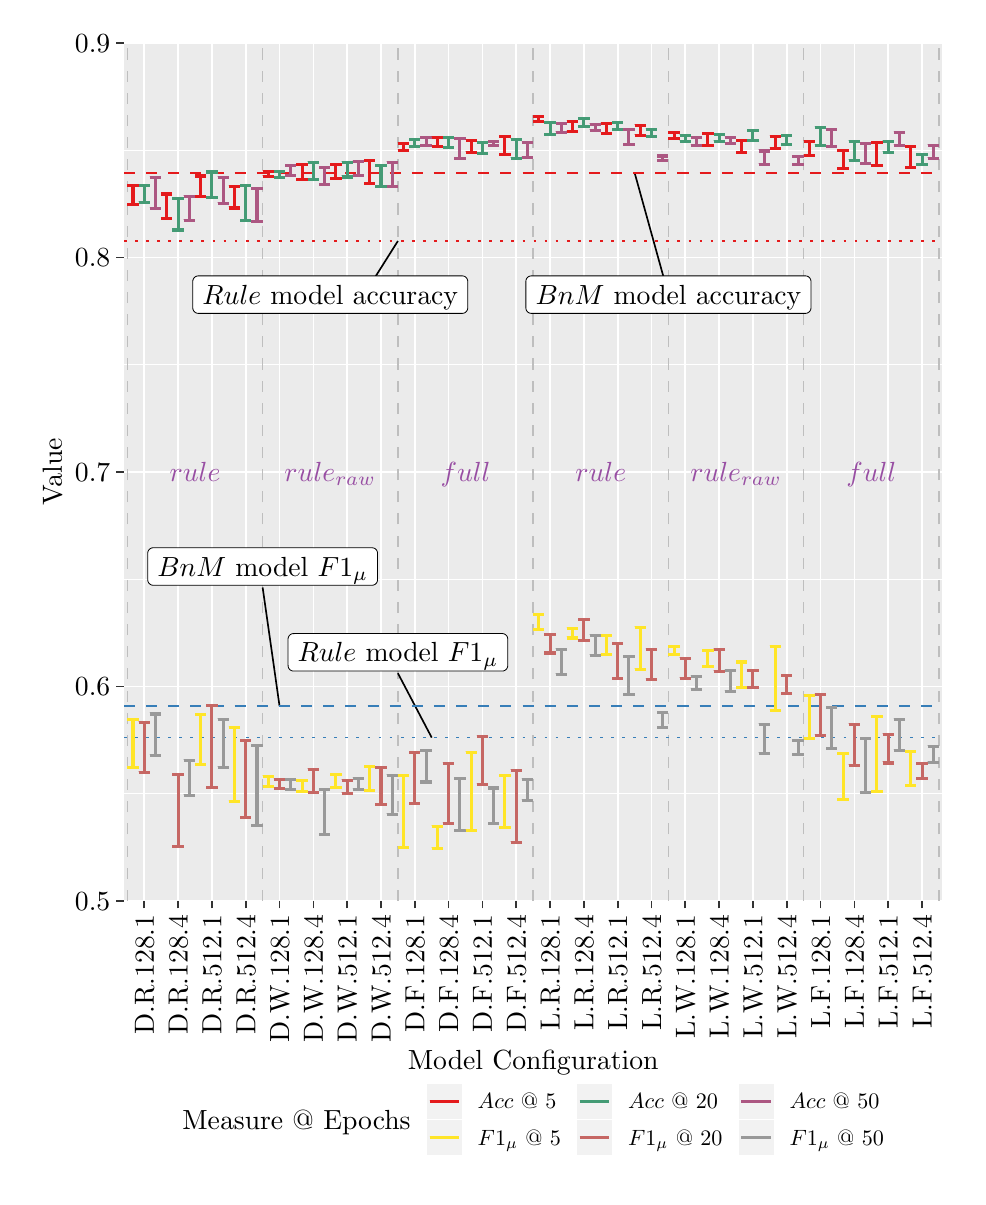
\begin{tikzpicture}[x=1pt,y=1pt]
\definecolor{fillColor}{RGB}{255,255,255}
\path[use as bounding box,fill=fillColor,fill opacity=0.00] (0,0) rectangle (336.00,415.30);
\begin{scope}
\path[clip] (  0.00,  0.00) rectangle (336.00,415.30);
\definecolor{drawColor}{RGB}{255,255,255}
\definecolor{fillColor}{RGB}{255,255,255}

\path[draw=drawColor,line width= 0.6pt,line join=round,line cap=round,fill=fillColor] (  0.00,  0.00) rectangle (336.00,415.30);
\end{scope}
\begin{scope}
\path[clip] ( 34.81, 99.77) rectangle (330.50,409.80);
\definecolor{fillColor}{gray}{0.92}

\path[fill=fillColor] ( 34.81, 99.77) rectangle (330.50,409.80);
\definecolor{drawColor}{RGB}{255,255,255}

\path[draw=drawColor,line width= 0.3pt,line join=round] ( 34.81,138.52) --
	(330.50,138.52);

\path[draw=drawColor,line width= 0.3pt,line join=round] ( 34.81,216.03) --
	(330.50,216.03);

\path[draw=drawColor,line width= 0.3pt,line join=round] ( 34.81,293.54) --
	(330.50,293.54);

\path[draw=drawColor,line width= 0.3pt,line join=round] ( 34.81,371.04) --
	(330.50,371.04);

\path[draw=drawColor,line width= 0.6pt,line join=round] ( 34.81, 99.77) --
	(330.50, 99.77);

\path[draw=drawColor,line width= 0.6pt,line join=round] ( 34.81,177.28) --
	(330.50,177.28);

\path[draw=drawColor,line width= 0.6pt,line join=round] ( 34.81,254.78) --
	(330.50,254.78);

\path[draw=drawColor,line width= 0.6pt,line join=round] ( 34.81,332.29) --
	(330.50,332.29);

\path[draw=drawColor,line width= 0.6pt,line join=round] ( 34.81,409.80) --
	(330.50,409.80);

\path[draw=drawColor,line width= 0.6pt,line join=round] ( 42.14, 99.77) --
	( 42.14,409.80);

\path[draw=drawColor,line width= 0.6pt,line join=round] ( 54.36, 99.77) --
	( 54.36,409.80);

\path[draw=drawColor,line width= 0.6pt,line join=round] ( 66.57, 99.77) --
	( 66.57,409.80);

\path[draw=drawColor,line width= 0.6pt,line join=round] ( 78.79, 99.77) --
	( 78.79,409.80);

\path[draw=drawColor,line width= 0.6pt,line join=round] ( 91.01, 99.77) --
	( 91.01,409.80);

\path[draw=drawColor,line width= 0.6pt,line join=round] (103.23, 99.77) --
	(103.23,409.80);

\path[draw=drawColor,line width= 0.6pt,line join=round] (115.45, 99.77) --
	(115.45,409.80);

\path[draw=drawColor,line width= 0.6pt,line join=round] (127.67, 99.77) --
	(127.67,409.80);

\path[draw=drawColor,line width= 0.6pt,line join=round] (139.89, 99.77) --
	(139.89,409.80);

\path[draw=drawColor,line width= 0.6pt,line join=round] (152.11, 99.77) --
	(152.11,409.80);

\path[draw=drawColor,line width= 0.6pt,line join=round] (164.32, 99.77) --
	(164.32,409.80);

\path[draw=drawColor,line width= 0.6pt,line join=round] (176.54, 99.77) --
	(176.54,409.80);

\path[draw=drawColor,line width= 0.6pt,line join=round] (188.76, 99.77) --
	(188.76,409.80);

\path[draw=drawColor,line width= 0.6pt,line join=round] (200.98, 99.77) --
	(200.98,409.80);

\path[draw=drawColor,line width= 0.6pt,line join=round] (213.20, 99.77) --
	(213.20,409.80);

\path[draw=drawColor,line width= 0.6pt,line join=round] (225.42, 99.77) --
	(225.42,409.80);

\path[draw=drawColor,line width= 0.6pt,line join=round] (237.64, 99.77) --
	(237.64,409.80);

\path[draw=drawColor,line width= 0.6pt,line join=round] (249.86, 99.77) --
	(249.86,409.80);

\path[draw=drawColor,line width= 0.6pt,line join=round] (262.07, 99.77) --
	(262.07,409.80);

\path[draw=drawColor,line width= 0.6pt,line join=round] (274.29, 99.77) --
	(274.29,409.80);

\path[draw=drawColor,line width= 0.6pt,line join=round] (286.51, 99.77) --
	(286.51,409.80);

\path[draw=drawColor,line width= 0.6pt,line join=round] (298.73, 99.77) --
	(298.73,409.80);

\path[draw=drawColor,line width= 0.6pt,line join=round] (310.95, 99.77) --
	(310.95,409.80);

\path[draw=drawColor,line width= 0.6pt,line join=round] (323.17, 99.77) --
	(323.17,409.80);
\definecolor{drawColor}{RGB}{190,190,190}

\path[draw=drawColor,line width= 0.6pt,dash pattern=on 4pt off 4pt ,line join=round] ( 36.03, 99.77) -- ( 36.03,409.80);

\path[draw=drawColor,line width= 0.6pt,dash pattern=on 4pt off 4pt ,line join=round] ( 84.90, 99.77) -- ( 84.90,409.80);

\path[draw=drawColor,line width= 0.6pt,dash pattern=on 4pt off 4pt ,line join=round] (133.78, 99.77) -- (133.78,409.80);

\path[draw=drawColor,line width= 0.6pt,dash pattern=on 4pt off 4pt ,line join=round] (182.65, 99.77) -- (182.65,409.80);

\path[draw=drawColor,line width= 0.6pt,dash pattern=on 4pt off 4pt ,line join=round] (231.53, 99.77) -- (231.53,409.80);

\path[draw=drawColor,line width= 0.6pt,dash pattern=on 4pt off 4pt ,line join=round] (280.40, 99.77) -- (280.40,409.80);

\path[draw=drawColor,line width= 0.6pt,dash pattern=on 4pt off 4pt ,line join=round] (329.28, 99.77) -- (329.28,409.80);
\definecolor{drawColor}{RGB}{152,78,163}

\node[text=drawColor,anchor=base,inner sep=0pt, outer sep=0pt, scale=  1.00] at ( 60.47,251.33) {\(rule\)};

\node[text=drawColor,anchor=base,inner sep=0pt, outer sep=0pt, scale=  1.00] at (109.34,251.33) {\(rule_{raw}\)};

\node[text=drawColor,anchor=base,inner sep=0pt, outer sep=0pt, scale=  1.00] at (158.22,251.33) {\(full\)};

\node[text=drawColor,anchor=base,inner sep=0pt, outer sep=0pt, scale=  1.00] at (207.09,251.33) {\(rule\)};

\node[text=drawColor,anchor=base,inner sep=0pt, outer sep=0pt, scale=  1.00] at (255.97,251.33) {\(rule_{raw}\)};

\node[text=drawColor,anchor=base,inner sep=0pt, outer sep=0pt, scale=  1.00] at (304.84,251.33) {\(full\)};
\definecolor{drawColor}{RGB}{0,0,0}

\path[draw=drawColor,line width= 0.6pt,line join=round] (121.56,318.83) --
	(133.78,338.21);

\path[draw=drawColor,line width= 0.6pt,line join=round] (219.31,362.90) --
	(231.53,318.83);

\path[draw=drawColor,line width= 0.6pt,line join=round] (133.78,182.02) --
	(146.00,158.77);

\path[draw=drawColor,line width= 0.6pt,line join=round] ( 84.90,213.02) --
	( 91.01,170.21);
\definecolor{fillColor}{RGB}{255,255,255}

\path[draw=drawColor,line width= 0.3pt,line join=round,line cap=round,fill=fillColor] ( 45.37,213.82) --
	(124.43,213.82) --
	(124.35,213.82) --
	(124.67,213.83) --
	(124.99,213.90) --
	(125.29,214.01) --
	(125.56,214.17) --
	(125.81,214.37) --
	(126.02,214.61) --
	(126.19,214.88) --
	(126.32,215.18) --
	(126.40,215.49) --
	(126.42,215.81) --
	(126.42,215.81) --
	(126.42,225.37) --
	(126.42,225.37) --
	(126.40,225.69) --
	(126.32,226.00) --
	(126.19,226.29) --
	(126.02,226.56) --
	(125.81,226.80) --
	(125.56,227.01) --
	(125.29,227.17) --
	(124.99,227.28) --
	(124.67,227.34) --
	(124.43,227.36) --
	( 45.37,227.36) --
	( 45.61,227.34) --
	( 45.29,227.36) --
	( 44.97,227.32) --
	( 44.67,227.23) --
	( 44.38,227.09) --
	( 44.11,226.91) --
	( 43.88,226.69) --
	( 43.69,226.43) --
	( 43.54,226.15) --
	( 43.44,225.85) --
	( 43.39,225.53) --
	( 43.38,225.37) --
	( 43.38,215.81) --
	( 43.39,215.97) --
	( 43.39,215.65) --
	( 43.44,215.33) --
	( 43.54,215.03) --
	( 43.69,214.74) --
	( 43.88,214.49) --
	( 44.11,214.27) --
	( 44.38,214.09) --
	( 44.67,213.95) --
	( 44.97,213.86) --
	( 45.29,213.82) --
	cycle;
\end{scope}
\begin{scope}
\path[clip] ( 34.81, 99.77) rectangle (330.50,409.80);
\definecolor{drawColor}{RGB}{0,0,0}

\node[text=drawColor,anchor=base,inner sep=0pt, outer sep=0pt, scale=  1.00] at ( 84.90,217.13) {\(BnM\) model \(F1_\mu\)};
\definecolor{fillColor}{RGB}{255,255,255}

\path[draw=drawColor,line width= 0.3pt,line join=round,line cap=round,fill=fillColor] ( 96.08,182.82) --
	(171.48,182.82) --
	(171.40,182.82) --
	(171.72,182.83) --
	(172.03,182.89) --
	(172.33,183.01) --
	(172.61,183.17) --
	(172.85,183.37) --
	(173.07,183.61) --
	(173.24,183.88) --
	(173.36,184.17) --
	(173.44,184.48) --
	(173.47,184.80) --
	(173.47,184.80) --
	(173.47,194.37) --
	(173.47,194.37) --
	(173.44,194.69) --
	(173.36,195.00) --
	(173.24,195.29) --
	(173.07,195.56) --
	(172.85,195.80) --
	(172.61,196.00) --
	(172.33,196.16) --
	(172.03,196.28) --
	(171.72,196.34) --
	(171.48,196.36) --
	( 96.08,196.36) --
	( 96.32,196.34) --
	( 96.00,196.35) --
	( 95.68,196.32) --
	( 95.37,196.23) --
	( 95.08,196.09) --
	( 94.82,195.91) --
	( 94.59,195.69) --
	( 94.40,195.43) --
	( 94.25,195.15) --
	( 94.15,194.84) --
	( 94.10,194.53) --
	( 94.09,194.37) --
	( 94.09,184.80) --
	( 94.10,184.96) --
	( 94.10,184.64) --
	( 94.15,184.33) --
	( 94.25,184.02) --
	( 94.40,183.74) --
	( 94.59,183.49) --
	( 94.82,183.26) --
	( 95.08,183.08) --
	( 95.37,182.95) --
	( 95.68,182.86) --
	( 96.00,182.82) --
	cycle;
\end{scope}
\begin{scope}
\path[clip] ( 34.81, 99.77) rectangle (330.50,409.80);
\definecolor{drawColor}{RGB}{0,0,0}

\node[text=drawColor,anchor=base,inner sep=0pt, outer sep=0pt, scale=  1.00] at (133.78,186.13) {\(Rule\) model \(F1_\mu\)};
\definecolor{fillColor}{RGB}{255,255,255}

\path[draw=drawColor,line width= 0.3pt,line join=round,line cap=round,fill=fillColor] ( 61.65,312.06) --
	(157.03,312.06) --
	(156.95,312.06) --
	(157.27,312.08) --
	(157.58,312.14) --
	(157.88,312.26) --
	(158.16,312.42) --
	(158.40,312.62) --
	(158.62,312.86) --
	(158.79,313.13) --
	(158.91,313.42) --
	(158.99,313.73) --
	(159.01,314.05) --
	(159.01,314.05) --
	(159.01,323.62) --
	(159.01,323.62) --
	(158.99,323.93) --
	(158.91,324.24) --
	(158.79,324.54) --
	(158.62,324.81) --
	(158.40,325.05) --
	(158.16,325.25) --
	(157.88,325.41) --
	(157.58,325.52) --
	(157.27,325.59) --
	(157.03,325.60) --
	( 61.65,325.60) --
	( 61.89,325.59) --
	( 61.57,325.60) --
	( 61.26,325.56) --
	( 60.95,325.47) --
	( 60.66,325.34) --
	( 60.40,325.15) --
	( 60.17,324.93) --
	( 59.97,324.68) --
	( 59.83,324.39) --
	( 59.72,324.09) --
	( 59.67,323.78) --
	( 59.67,323.62) --
	( 59.67,314.05) --
	( 59.67,314.21) --
	( 59.67,313.89) --
	( 59.72,313.58) --
	( 59.83,313.27) --
	( 59.97,312.99) --
	( 60.17,312.73) --
	( 60.40,312.51) --
	( 60.66,312.33) --
	( 60.95,312.19) --
	( 61.26,312.10) --
	( 61.57,312.06) --
	cycle;
\end{scope}
\begin{scope}
\path[clip] ( 34.81, 99.77) rectangle (330.50,409.80);
\definecolor{drawColor}{RGB}{0,0,0}

\node[text=drawColor,anchor=base,inner sep=0pt, outer sep=0pt, scale=  1.00] at (109.34,315.38) {\(Rule\) model accuracy};
\definecolor{fillColor}{RGB}{255,255,255}

\path[draw=drawColor,line width= 0.3pt,line join=round,line cap=round,fill=fillColor] (182.01,312.06) --
	(281.05,312.06) --
	(280.97,312.06) --
	(281.29,312.08) --
	(281.60,312.14) --
	(281.90,312.26) --
	(282.17,312.42) --
	(282.42,312.62) --
	(282.63,312.86) --
	(282.81,313.13) --
	(282.93,313.42) --
	(283.01,313.73) --
	(283.03,314.05) --
	(283.03,314.05) --
	(283.03,323.62) --
	(283.03,323.62) --
	(283.01,323.93) --
	(282.93,324.24) --
	(282.81,324.54) --
	(282.63,324.81) --
	(282.42,325.05) --
	(282.17,325.25) --
	(281.90,325.41) --
	(281.60,325.52) --
	(281.29,325.59) --
	(281.05,325.60) --
	(182.01,325.60) --
	(182.25,325.59) --
	(181.93,325.60) --
	(181.61,325.56) --
	(181.31,325.47) --
	(181.02,325.34) --
	(180.75,325.15) --
	(180.52,324.93) --
	(180.33,324.68) --
	(180.18,324.39) --
	(180.08,324.09) --
	(180.03,323.78) --
	(180.02,323.62) --
	(180.02,314.05) --
	(180.03,314.21) --
	(180.03,313.89) --
	(180.08,313.58) --
	(180.18,313.27) --
	(180.33,312.99) --
	(180.52,312.73) --
	(180.75,312.51) --
	(181.02,312.33) --
	(181.31,312.19) --
	(181.61,312.10) --
	(181.93,312.06) --
	cycle;
\end{scope}
\begin{scope}
\path[clip] ( 34.81, 99.77) rectangle (330.50,409.80);
\definecolor{drawColor}{RGB}{0,0,0}

\node[text=drawColor,anchor=base,inner sep=0pt, outer sep=0pt, scale=  1.00] at (231.53,315.38) {\(BnM\) model accuracy};
\definecolor{drawColor}{RGB}{228,26,28}

\path[draw=drawColor,line width= 0.6pt,dash pattern=on 4pt off 4pt ,line join=round] ( 34.81,362.90) -- (330.50,362.90);

\path[draw=drawColor,line width= 0.6pt,dash pattern=on 1pt off 3pt ,line join=round] ( 34.81,338.21) -- (330.50,338.21);
\definecolor{drawColor}{RGB}{55,126,184}

\path[draw=drawColor,line width= 0.6pt,dash pattern=on 4pt off 4pt ,line join=round] ( 34.81,170.21) -- (330.50,170.21);

\path[draw=drawColor,line width= 0.6pt,dash pattern=on 1pt off 3pt ,line join=round] ( 34.81,158.77) -- (330.50,158.77);
\definecolor{drawColor}{RGB}{172,87,130}

\path[draw=drawColor,line width= 1.1pt,line join=round] ( 44.17,361.20) --
	( 48.25,361.20);

\path[draw=drawColor,line width= 1.1pt,line join=round] ( 46.21,361.20) --
	( 46.21,350.00);

\path[draw=drawColor,line width= 1.1pt,line join=round] ( 44.17,350.00) --
	( 48.25,350.00);

\path[draw=drawColor,line width= 1.1pt,line join=round] ( 44.17,361.20) --
	( 48.25,361.20);

\path[draw=drawColor,line width= 1.1pt,line join=round] ( 46.21,361.20) --
	( 46.21,350.00);

\path[draw=drawColor,line width= 1.1pt,line join=round] ( 44.17,350.00) --
	( 48.25,350.00);

\path[draw=drawColor,line width= 1.1pt,line join=round] ( 44.17,361.20) --
	( 48.25,361.20);

\path[draw=drawColor,line width= 1.1pt,line join=round] ( 46.21,361.20) --
	( 46.21,350.00);

\path[draw=drawColor,line width= 1.1pt,line join=round] ( 44.17,350.00) --
	( 48.25,350.00);

\path[draw=drawColor,line width= 1.1pt,line join=round] ( 44.17,361.20) --
	( 48.25,361.20);

\path[draw=drawColor,line width= 1.1pt,line join=round] ( 46.21,361.20) --
	( 46.21,350.00);

\path[draw=drawColor,line width= 1.1pt,line join=round] ( 44.17,350.00) --
	( 48.25,350.00);

\path[draw=drawColor,line width= 1.1pt,line join=round] ( 44.17,361.20) --
	( 48.25,361.20);

\path[draw=drawColor,line width= 1.1pt,line join=round] ( 46.21,361.20) --
	( 46.21,350.00);

\path[draw=drawColor,line width= 1.1pt,line join=round] ( 44.17,350.00) --
	( 48.25,350.00);

\path[draw=drawColor,line width= 1.1pt,line join=round] ( 44.17,361.20) --
	( 48.25,361.20);

\path[draw=drawColor,line width= 1.1pt,line join=round] ( 46.21,361.20) --
	( 46.21,350.00);

\path[draw=drawColor,line width= 1.1pt,line join=round] ( 44.17,350.00) --
	( 48.25,350.00);

\path[draw=drawColor,line width= 1.1pt,line join=round] ( 44.17,361.20) --
	( 48.25,361.20);

\path[draw=drawColor,line width= 1.1pt,line join=round] ( 46.21,361.20) --
	( 46.21,350.00);

\path[draw=drawColor,line width= 1.1pt,line join=round] ( 44.17,350.00) --
	( 48.25,350.00);

\path[draw=drawColor,line width= 1.1pt,line join=round] ( 44.17,361.20) --
	( 48.25,361.20);

\path[draw=drawColor,line width= 1.1pt,line join=round] ( 46.21,361.20) --
	( 46.21,350.00);

\path[draw=drawColor,line width= 1.1pt,line join=round] ( 44.17,350.00) --
	( 48.25,350.00);
\definecolor{drawColor}{RGB}{68,155,117}

\path[draw=drawColor,line width= 1.1pt,line join=round] ( 40.10,358.33) --
	( 44.17,358.33);

\path[draw=drawColor,line width= 1.1pt,line join=round] ( 42.14,358.33) --
	( 42.14,352.15);

\path[draw=drawColor,line width= 1.1pt,line join=round] ( 40.10,352.15) --
	( 44.17,352.15);

\path[draw=drawColor,line width= 1.1pt,line join=round] ( 40.10,358.33) --
	( 44.17,358.33);

\path[draw=drawColor,line width= 1.1pt,line join=round] ( 42.14,358.33) --
	( 42.14,352.15);

\path[draw=drawColor,line width= 1.1pt,line join=round] ( 40.10,352.15) --
	( 44.17,352.15);

\path[draw=drawColor,line width= 1.1pt,line join=round] ( 40.10,358.33) --
	( 44.17,358.33);

\path[draw=drawColor,line width= 1.1pt,line join=round] ( 42.14,358.33) --
	( 42.14,352.15);

\path[draw=drawColor,line width= 1.1pt,line join=round] ( 40.10,352.15) --
	( 44.17,352.15);

\path[draw=drawColor,line width= 1.1pt,line join=round] ( 40.10,358.33) --
	( 44.17,358.33);

\path[draw=drawColor,line width= 1.1pt,line join=round] ( 42.14,358.33) --
	( 42.14,352.15);

\path[draw=drawColor,line width= 1.1pt,line join=round] ( 40.10,352.15) --
	( 44.17,352.15);

\path[draw=drawColor,line width= 1.1pt,line join=round] ( 40.10,358.33) --
	( 44.17,358.33);

\path[draw=drawColor,line width= 1.1pt,line join=round] ( 42.14,358.33) --
	( 42.14,352.15);

\path[draw=drawColor,line width= 1.1pt,line join=round] ( 40.10,352.15) --
	( 44.17,352.15);

\path[draw=drawColor,line width= 1.1pt,line join=round] ( 40.10,358.33) --
	( 44.17,358.33);

\path[draw=drawColor,line width= 1.1pt,line join=round] ( 42.14,358.33) --
	( 42.14,352.15);

\path[draw=drawColor,line width= 1.1pt,line join=round] ( 40.10,352.15) --
	( 44.17,352.15);

\path[draw=drawColor,line width= 1.1pt,line join=round] ( 40.10,358.33) --
	( 44.17,358.33);

\path[draw=drawColor,line width= 1.1pt,line join=round] ( 42.14,358.33) --
	( 42.14,352.15);

\path[draw=drawColor,line width= 1.1pt,line join=round] ( 40.10,352.15) --
	( 44.17,352.15);

\path[draw=drawColor,line width= 1.1pt,line join=round] ( 40.10,358.33) --
	( 44.17,358.33);

\path[draw=drawColor,line width= 1.1pt,line join=round] ( 42.14,358.33) --
	( 42.14,352.15);

\path[draw=drawColor,line width= 1.1pt,line join=round] ( 40.10,352.15) --
	( 44.17,352.15);
\definecolor{drawColor}{RGB}{228,26,28}

\path[draw=drawColor,line width= 1.1pt,line join=round] ( 36.03,358.29) --
	( 40.10,358.29);

\path[draw=drawColor,line width= 1.1pt,line join=round] ( 38.06,358.29) --
	( 38.06,351.37);

\path[draw=drawColor,line width= 1.1pt,line join=round] ( 36.03,351.37) --
	( 40.10,351.37);

\path[draw=drawColor,line width= 1.1pt,line join=round] ( 36.03,358.29) --
	( 40.10,358.29);

\path[draw=drawColor,line width= 1.1pt,line join=round] ( 38.06,358.29) --
	( 38.06,351.37);

\path[draw=drawColor,line width= 1.1pt,line join=round] ( 36.03,351.37) --
	( 40.10,351.37);

\path[draw=drawColor,line width= 1.1pt,line join=round] ( 36.03,358.29) --
	( 40.10,358.29);

\path[draw=drawColor,line width= 1.1pt,line join=round] ( 38.06,358.29) --
	( 38.06,351.37);

\path[draw=drawColor,line width= 1.1pt,line join=round] ( 36.03,351.37) --
	( 40.10,351.37);

\path[draw=drawColor,line width= 1.1pt,line join=round] ( 36.03,358.29) --
	( 40.10,358.29);

\path[draw=drawColor,line width= 1.1pt,line join=round] ( 38.06,358.29) --
	( 38.06,351.37);

\path[draw=drawColor,line width= 1.1pt,line join=round] ( 36.03,351.37) --
	( 40.10,351.37);

\path[draw=drawColor,line width= 1.1pt,line join=round] ( 36.03,358.29) --
	( 40.10,358.29);

\path[draw=drawColor,line width= 1.1pt,line join=round] ( 38.06,358.29) --
	( 38.06,351.37);

\path[draw=drawColor,line width= 1.1pt,line join=round] ( 36.03,351.37) --
	( 40.10,351.37);

\path[draw=drawColor,line width= 1.1pt,line join=round] ( 36.03,358.29) --
	( 40.10,358.29);

\path[draw=drawColor,line width= 1.1pt,line join=round] ( 38.06,358.29) --
	( 38.06,351.37);

\path[draw=drawColor,line width= 1.1pt,line join=round] ( 36.03,351.37) --
	( 40.10,351.37);

\path[draw=drawColor,line width= 1.1pt,line join=round] ( 36.03,358.29) --
	( 40.10,358.29);

\path[draw=drawColor,line width= 1.1pt,line join=round] ( 38.06,358.29) --
	( 38.06,351.37);

\path[draw=drawColor,line width= 1.1pt,line join=round] ( 36.03,351.37) --
	( 40.10,351.37);

\path[draw=drawColor,line width= 1.1pt,line join=round] ( 36.03,358.29) --
	( 40.10,358.29);

\path[draw=drawColor,line width= 1.1pt,line join=round] ( 38.06,358.29) --
	( 38.06,351.37);

\path[draw=drawColor,line width= 1.1pt,line join=round] ( 36.03,351.37) --
	( 40.10,351.37);
\definecolor{drawColor}{RGB}{172,87,130}

\path[draw=drawColor,line width= 1.1pt,line join=round] ( 56.39,354.20) --
	( 60.47,354.20);

\path[draw=drawColor,line width= 1.1pt,line join=round] ( 58.43,354.20) --
	( 58.43,345.45);

\path[draw=drawColor,line width= 1.1pt,line join=round] ( 56.39,345.45) --
	( 60.47,345.45);

\path[draw=drawColor,line width= 1.1pt,line join=round] ( 56.39,354.20) --
	( 60.47,354.20);

\path[draw=drawColor,line width= 1.1pt,line join=round] ( 58.43,354.20) --
	( 58.43,345.45);

\path[draw=drawColor,line width= 1.1pt,line join=round] ( 56.39,345.45) --
	( 60.47,345.45);

\path[draw=drawColor,line width= 1.1pt,line join=round] ( 56.39,354.20) --
	( 60.47,354.20);

\path[draw=drawColor,line width= 1.1pt,line join=round] ( 58.43,354.20) --
	( 58.43,345.45);

\path[draw=drawColor,line width= 1.1pt,line join=round] ( 56.39,345.45) --
	( 60.47,345.45);

\path[draw=drawColor,line width= 1.1pt,line join=round] ( 56.39,354.20) --
	( 60.47,354.20);

\path[draw=drawColor,line width= 1.1pt,line join=round] ( 58.43,354.20) --
	( 58.43,345.45);

\path[draw=drawColor,line width= 1.1pt,line join=round] ( 56.39,345.45) --
	( 60.47,345.45);

\path[draw=drawColor,line width= 1.1pt,line join=round] ( 56.39,354.20) --
	( 60.47,354.20);

\path[draw=drawColor,line width= 1.1pt,line join=round] ( 58.43,354.20) --
	( 58.43,345.45);

\path[draw=drawColor,line width= 1.1pt,line join=round] ( 56.39,345.45) --
	( 60.47,345.45);

\path[draw=drawColor,line width= 1.1pt,line join=round] ( 56.39,354.20) --
	( 60.47,354.20);

\path[draw=drawColor,line width= 1.1pt,line join=round] ( 58.43,354.20) --
	( 58.43,345.45);

\path[draw=drawColor,line width= 1.1pt,line join=round] ( 56.39,345.45) --
	( 60.47,345.45);

\path[draw=drawColor,line width= 1.1pt,line join=round] ( 56.39,354.20) --
	( 60.47,354.20);

\path[draw=drawColor,line width= 1.1pt,line join=round] ( 58.43,354.20) --
	( 58.43,345.45);

\path[draw=drawColor,line width= 1.1pt,line join=round] ( 56.39,345.45) --
	( 60.47,345.45);

\path[draw=drawColor,line width= 1.1pt,line join=round] ( 56.39,354.20) --
	( 60.47,354.20);

\path[draw=drawColor,line width= 1.1pt,line join=round] ( 58.43,354.20) --
	( 58.43,345.45);

\path[draw=drawColor,line width= 1.1pt,line join=round] ( 56.39,345.45) --
	( 60.47,345.45);
\definecolor{drawColor}{RGB}{68,155,117}

\path[draw=drawColor,line width= 1.1pt,line join=round] ( 52.32,353.59) --
	( 56.39,353.59);

\path[draw=drawColor,line width= 1.1pt,line join=round] ( 54.36,353.59) --
	( 54.36,342.19);

\path[draw=drawColor,line width= 1.1pt,line join=round] ( 52.32,342.19) --
	( 56.39,342.19);

\path[draw=drawColor,line width= 1.1pt,line join=round] ( 52.32,353.59) --
	( 56.39,353.59);

\path[draw=drawColor,line width= 1.1pt,line join=round] ( 54.36,353.59) --
	( 54.36,342.19);

\path[draw=drawColor,line width= 1.1pt,line join=round] ( 52.32,342.19) --
	( 56.39,342.19);

\path[draw=drawColor,line width= 1.1pt,line join=round] ( 52.32,353.59) --
	( 56.39,353.59);

\path[draw=drawColor,line width= 1.1pt,line join=round] ( 54.36,353.59) --
	( 54.36,342.19);

\path[draw=drawColor,line width= 1.1pt,line join=round] ( 52.32,342.19) --
	( 56.39,342.19);

\path[draw=drawColor,line width= 1.1pt,line join=round] ( 52.32,353.59) --
	( 56.39,353.59);

\path[draw=drawColor,line width= 1.1pt,line join=round] ( 54.36,353.59) --
	( 54.36,342.19);

\path[draw=drawColor,line width= 1.1pt,line join=round] ( 52.32,342.19) --
	( 56.39,342.19);

\path[draw=drawColor,line width= 1.1pt,line join=round] ( 52.32,353.59) --
	( 56.39,353.59);

\path[draw=drawColor,line width= 1.1pt,line join=round] ( 54.36,353.59) --
	( 54.36,342.19);

\path[draw=drawColor,line width= 1.1pt,line join=round] ( 52.32,342.19) --
	( 56.39,342.19);

\path[draw=drawColor,line width= 1.1pt,line join=round] ( 52.32,353.59) --
	( 56.39,353.59);

\path[draw=drawColor,line width= 1.1pt,line join=round] ( 54.36,353.59) --
	( 54.36,342.19);

\path[draw=drawColor,line width= 1.1pt,line join=round] ( 52.32,342.19) --
	( 56.39,342.19);

\path[draw=drawColor,line width= 1.1pt,line join=round] ( 52.32,353.59) --
	( 56.39,353.59);

\path[draw=drawColor,line width= 1.1pt,line join=round] ( 54.36,353.59) --
	( 54.36,342.19);

\path[draw=drawColor,line width= 1.1pt,line join=round] ( 52.32,342.19) --
	( 56.39,342.19);

\path[draw=drawColor,line width= 1.1pt,line join=round] ( 52.32,353.59) --
	( 56.39,353.59);

\path[draw=drawColor,line width= 1.1pt,line join=round] ( 54.36,353.59) --
	( 54.36,342.19);

\path[draw=drawColor,line width= 1.1pt,line join=round] ( 52.32,342.19) --
	( 56.39,342.19);
\definecolor{drawColor}{RGB}{228,26,28}

\path[draw=drawColor,line width= 1.1pt,line join=round] ( 48.25,355.19) --
	( 52.32,355.19);

\path[draw=drawColor,line width= 1.1pt,line join=round] ( 50.28,355.19) --
	( 50.28,346.26);

\path[draw=drawColor,line width= 1.1pt,line join=round] ( 48.25,346.26) --
	( 52.32,346.26);

\path[draw=drawColor,line width= 1.1pt,line join=round] ( 48.25,355.19) --
	( 52.32,355.19);

\path[draw=drawColor,line width= 1.1pt,line join=round] ( 50.28,355.19) --
	( 50.28,346.26);

\path[draw=drawColor,line width= 1.1pt,line join=round] ( 48.25,346.26) --
	( 52.32,346.26);

\path[draw=drawColor,line width= 1.1pt,line join=round] ( 48.25,355.19) --
	( 52.32,355.19);

\path[draw=drawColor,line width= 1.1pt,line join=round] ( 50.28,355.19) --
	( 50.28,346.26);

\path[draw=drawColor,line width= 1.1pt,line join=round] ( 48.25,346.26) --
	( 52.32,346.26);

\path[draw=drawColor,line width= 1.1pt,line join=round] ( 48.25,355.19) --
	( 52.32,355.19);

\path[draw=drawColor,line width= 1.1pt,line join=round] ( 50.28,355.19) --
	( 50.28,346.26);

\path[draw=drawColor,line width= 1.1pt,line join=round] ( 48.25,346.26) --
	( 52.32,346.26);

\path[draw=drawColor,line width= 1.1pt,line join=round] ( 48.25,355.19) --
	( 52.32,355.19);

\path[draw=drawColor,line width= 1.1pt,line join=round] ( 50.28,355.19) --
	( 50.28,346.26);

\path[draw=drawColor,line width= 1.1pt,line join=round] ( 48.25,346.26) --
	( 52.32,346.26);

\path[draw=drawColor,line width= 1.1pt,line join=round] ( 48.25,355.19) --
	( 52.32,355.19);

\path[draw=drawColor,line width= 1.1pt,line join=round] ( 50.28,355.19) --
	( 50.28,346.26);

\path[draw=drawColor,line width= 1.1pt,line join=round] ( 48.25,346.26) --
	( 52.32,346.26);

\path[draw=drawColor,line width= 1.1pt,line join=round] ( 48.25,355.19) --
	( 52.32,355.19);

\path[draw=drawColor,line width= 1.1pt,line join=round] ( 50.28,355.19) --
	( 50.28,346.26);

\path[draw=drawColor,line width= 1.1pt,line join=round] ( 48.25,346.26) --
	( 52.32,346.26);

\path[draw=drawColor,line width= 1.1pt,line join=round] ( 48.25,355.19) --
	( 52.32,355.19);

\path[draw=drawColor,line width= 1.1pt,line join=round] ( 50.28,355.19) --
	( 50.28,346.26);

\path[draw=drawColor,line width= 1.1pt,line join=round] ( 48.25,346.26) --
	( 52.32,346.26);
\definecolor{drawColor}{RGB}{172,87,130}

\path[draw=drawColor,line width= 1.1pt,line join=round] ( 68.61,361.02) --
	( 72.68,361.02);

\path[draw=drawColor,line width= 1.1pt,line join=round] ( 70.65,361.02) --
	( 70.65,351.70);

\path[draw=drawColor,line width= 1.1pt,line join=round] ( 68.61,351.70) --
	( 72.68,351.70);

\path[draw=drawColor,line width= 1.1pt,line join=round] ( 68.61,361.02) --
	( 72.68,361.02);

\path[draw=drawColor,line width= 1.1pt,line join=round] ( 70.65,361.02) --
	( 70.65,351.70);

\path[draw=drawColor,line width= 1.1pt,line join=round] ( 68.61,351.70) --
	( 72.68,351.70);

\path[draw=drawColor,line width= 1.1pt,line join=round] ( 68.61,361.02) --
	( 72.68,361.02);

\path[draw=drawColor,line width= 1.1pt,line join=round] ( 70.65,361.02) --
	( 70.65,351.70);

\path[draw=drawColor,line width= 1.1pt,line join=round] ( 68.61,351.70) --
	( 72.68,351.70);

\path[draw=drawColor,line width= 1.1pt,line join=round] ( 68.61,361.02) --
	( 72.68,361.02);

\path[draw=drawColor,line width= 1.1pt,line join=round] ( 70.65,361.02) --
	( 70.65,351.70);

\path[draw=drawColor,line width= 1.1pt,line join=round] ( 68.61,351.70) --
	( 72.68,351.70);

\path[draw=drawColor,line width= 1.1pt,line join=round] ( 68.61,361.02) --
	( 72.68,361.02);

\path[draw=drawColor,line width= 1.1pt,line join=round] ( 70.65,361.02) --
	( 70.65,351.70);

\path[draw=drawColor,line width= 1.1pt,line join=round] ( 68.61,351.70) --
	( 72.68,351.70);

\path[draw=drawColor,line width= 1.1pt,line join=round] ( 68.61,361.02) --
	( 72.68,361.02);

\path[draw=drawColor,line width= 1.1pt,line join=round] ( 70.65,361.02) --
	( 70.65,351.70);

\path[draw=drawColor,line width= 1.1pt,line join=round] ( 68.61,351.70) --
	( 72.68,351.70);

\path[draw=drawColor,line width= 1.1pt,line join=round] ( 68.61,361.02) --
	( 72.68,361.02);

\path[draw=drawColor,line width= 1.1pt,line join=round] ( 70.65,361.02) --
	( 70.65,351.70);

\path[draw=drawColor,line width= 1.1pt,line join=round] ( 68.61,351.70) --
	( 72.68,351.70);

\path[draw=drawColor,line width= 1.1pt,line join=round] ( 68.61,361.02) --
	( 72.68,361.02);

\path[draw=drawColor,line width= 1.1pt,line join=round] ( 70.65,361.02) --
	( 70.65,351.70);

\path[draw=drawColor,line width= 1.1pt,line join=round] ( 68.61,351.70) --
	( 72.68,351.70);
\definecolor{drawColor}{RGB}{68,155,117}

\path[draw=drawColor,line width= 1.1pt,line join=round] ( 64.54,363.15) --
	( 68.61,363.15);

\path[draw=drawColor,line width= 1.1pt,line join=round] ( 66.57,363.15) --
	( 66.57,353.98);

\path[draw=drawColor,line width= 1.1pt,line join=round] ( 64.54,353.98) --
	( 68.61,353.98);

\path[draw=drawColor,line width= 1.1pt,line join=round] ( 64.54,363.15) --
	( 68.61,363.15);

\path[draw=drawColor,line width= 1.1pt,line join=round] ( 66.57,363.15) --
	( 66.57,353.98);

\path[draw=drawColor,line width= 1.1pt,line join=round] ( 64.54,353.98) --
	( 68.61,353.98);

\path[draw=drawColor,line width= 1.1pt,line join=round] ( 64.54,363.15) --
	( 68.61,363.15);

\path[draw=drawColor,line width= 1.1pt,line join=round] ( 66.57,363.15) --
	( 66.57,353.98);

\path[draw=drawColor,line width= 1.1pt,line join=round] ( 64.54,353.98) --
	( 68.61,353.98);

\path[draw=drawColor,line width= 1.1pt,line join=round] ( 64.54,363.15) --
	( 68.61,363.15);

\path[draw=drawColor,line width= 1.1pt,line join=round] ( 66.57,363.15) --
	( 66.57,353.98);

\path[draw=drawColor,line width= 1.1pt,line join=round] ( 64.54,353.98) --
	( 68.61,353.98);

\path[draw=drawColor,line width= 1.1pt,line join=round] ( 64.54,363.15) --
	( 68.61,363.15);

\path[draw=drawColor,line width= 1.1pt,line join=round] ( 66.57,363.15) --
	( 66.57,353.98);

\path[draw=drawColor,line width= 1.1pt,line join=round] ( 64.54,353.98) --
	( 68.61,353.98);

\path[draw=drawColor,line width= 1.1pt,line join=round] ( 64.54,363.15) --
	( 68.61,363.15);

\path[draw=drawColor,line width= 1.1pt,line join=round] ( 66.57,363.15) --
	( 66.57,353.98);

\path[draw=drawColor,line width= 1.1pt,line join=round] ( 64.54,353.98) --
	( 68.61,353.98);

\path[draw=drawColor,line width= 1.1pt,line join=round] ( 64.54,363.15) --
	( 68.61,363.15);

\path[draw=drawColor,line width= 1.1pt,line join=round] ( 66.57,363.15) --
	( 66.57,353.98);

\path[draw=drawColor,line width= 1.1pt,line join=round] ( 64.54,353.98) --
	( 68.61,353.98);

\path[draw=drawColor,line width= 1.1pt,line join=round] ( 64.54,363.15) --
	( 68.61,363.15);

\path[draw=drawColor,line width= 1.1pt,line join=round] ( 66.57,363.15) --
	( 66.57,353.98);

\path[draw=drawColor,line width= 1.1pt,line join=round] ( 64.54,353.98) --
	( 68.61,353.98);
\definecolor{drawColor}{RGB}{228,26,28}

\path[draw=drawColor,line width= 1.1pt,line join=round] ( 60.47,361.70) --
	( 64.54,361.70);

\path[draw=drawColor,line width= 1.1pt,line join=round] ( 62.50,361.70) --
	( 62.50,354.45);

\path[draw=drawColor,line width= 1.1pt,line join=round] ( 60.47,354.45) --
	( 64.54,354.45);

\path[draw=drawColor,line width= 1.1pt,line join=round] ( 60.47,361.70) --
	( 64.54,361.70);

\path[draw=drawColor,line width= 1.1pt,line join=round] ( 62.50,361.70) --
	( 62.50,354.45);

\path[draw=drawColor,line width= 1.1pt,line join=round] ( 60.47,354.45) --
	( 64.54,354.45);

\path[draw=drawColor,line width= 1.1pt,line join=round] ( 60.47,361.70) --
	( 64.54,361.70);

\path[draw=drawColor,line width= 1.1pt,line join=round] ( 62.50,361.70) --
	( 62.50,354.45);

\path[draw=drawColor,line width= 1.1pt,line join=round] ( 60.47,354.45) --
	( 64.54,354.45);

\path[draw=drawColor,line width= 1.1pt,line join=round] ( 60.47,361.70) --
	( 64.54,361.70);

\path[draw=drawColor,line width= 1.1pt,line join=round] ( 62.50,361.70) --
	( 62.50,354.45);

\path[draw=drawColor,line width= 1.1pt,line join=round] ( 60.47,354.45) --
	( 64.54,354.45);

\path[draw=drawColor,line width= 1.1pt,line join=round] ( 60.47,361.70) --
	( 64.54,361.70);

\path[draw=drawColor,line width= 1.1pt,line join=round] ( 62.50,361.70) --
	( 62.50,354.45);

\path[draw=drawColor,line width= 1.1pt,line join=round] ( 60.47,354.45) --
	( 64.54,354.45);

\path[draw=drawColor,line width= 1.1pt,line join=round] ( 60.47,361.70) --
	( 64.54,361.70);

\path[draw=drawColor,line width= 1.1pt,line join=round] ( 62.50,361.70) --
	( 62.50,354.45);

\path[draw=drawColor,line width= 1.1pt,line join=round] ( 60.47,354.45) --
	( 64.54,354.45);

\path[draw=drawColor,line width= 1.1pt,line join=round] ( 60.47,361.70) --
	( 64.54,361.70);

\path[draw=drawColor,line width= 1.1pt,line join=round] ( 62.50,361.70) --
	( 62.50,354.45);

\path[draw=drawColor,line width= 1.1pt,line join=round] ( 60.47,354.45) --
	( 64.54,354.45);

\path[draw=drawColor,line width= 1.1pt,line join=round] ( 60.47,361.70) --
	( 64.54,361.70);

\path[draw=drawColor,line width= 1.1pt,line join=round] ( 62.50,361.70) --
	( 62.50,354.45);

\path[draw=drawColor,line width= 1.1pt,line join=round] ( 60.47,354.45) --
	( 64.54,354.45);
\definecolor{drawColor}{RGB}{172,87,130}

\path[draw=drawColor,line width= 1.1pt,line join=round] ( 80.83,357.27) --
	( 84.90,357.27);

\path[draw=drawColor,line width= 1.1pt,line join=round] ( 82.87,357.27) --
	( 82.87,345.28);

\path[draw=drawColor,line width= 1.1pt,line join=round] ( 80.83,345.28) --
	( 84.90,345.28);

\path[draw=drawColor,line width= 1.1pt,line join=round] ( 80.83,357.27) --
	( 84.90,357.27);

\path[draw=drawColor,line width= 1.1pt,line join=round] ( 82.87,357.27) --
	( 82.87,345.28);

\path[draw=drawColor,line width= 1.1pt,line join=round] ( 80.83,345.28) --
	( 84.90,345.28);

\path[draw=drawColor,line width= 1.1pt,line join=round] ( 80.83,357.27) --
	( 84.90,357.27);

\path[draw=drawColor,line width= 1.1pt,line join=round] ( 82.87,357.27) --
	( 82.87,345.28);

\path[draw=drawColor,line width= 1.1pt,line join=round] ( 80.83,345.28) --
	( 84.90,345.28);

\path[draw=drawColor,line width= 1.1pt,line join=round] ( 80.83,357.27) --
	( 84.90,357.27);

\path[draw=drawColor,line width= 1.1pt,line join=round] ( 82.87,357.27) --
	( 82.87,345.28);

\path[draw=drawColor,line width= 1.1pt,line join=round] ( 80.83,345.28) --
	( 84.90,345.28);

\path[draw=drawColor,line width= 1.1pt,line join=round] ( 80.83,357.27) --
	( 84.90,357.27);

\path[draw=drawColor,line width= 1.1pt,line join=round] ( 82.87,357.27) --
	( 82.87,345.28);

\path[draw=drawColor,line width= 1.1pt,line join=round] ( 80.83,345.28) --
	( 84.90,345.28);

\path[draw=drawColor,line width= 1.1pt,line join=round] ( 80.83,357.27) --
	( 84.90,357.27);

\path[draw=drawColor,line width= 1.1pt,line join=round] ( 82.87,357.27) --
	( 82.87,345.28);

\path[draw=drawColor,line width= 1.1pt,line join=round] ( 80.83,345.28) --
	( 84.90,345.28);

\path[draw=drawColor,line width= 1.1pt,line join=round] ( 80.83,357.27) --
	( 84.90,357.27);

\path[draw=drawColor,line width= 1.1pt,line join=round] ( 82.87,357.27) --
	( 82.87,345.28);

\path[draw=drawColor,line width= 1.1pt,line join=round] ( 80.83,345.28) --
	( 84.90,345.28);

\path[draw=drawColor,line width= 1.1pt,line join=round] ( 80.83,357.27) --
	( 84.90,357.27);

\path[draw=drawColor,line width= 1.1pt,line join=round] ( 82.87,357.27) --
	( 82.87,345.28);

\path[draw=drawColor,line width= 1.1pt,line join=round] ( 80.83,345.28) --
	( 84.90,345.28);
\definecolor{drawColor}{RGB}{68,155,117}

\path[draw=drawColor,line width= 1.1pt,line join=round] ( 76.76,358.27) --
	( 80.83,358.27);

\path[draw=drawColor,line width= 1.1pt,line join=round] ( 78.79,358.27) --
	( 78.79,345.55);

\path[draw=drawColor,line width= 1.1pt,line join=round] ( 76.76,345.55) --
	( 80.83,345.55);

\path[draw=drawColor,line width= 1.1pt,line join=round] ( 76.76,358.27) --
	( 80.83,358.27);

\path[draw=drawColor,line width= 1.1pt,line join=round] ( 78.79,358.27) --
	( 78.79,345.55);

\path[draw=drawColor,line width= 1.1pt,line join=round] ( 76.76,345.55) --
	( 80.83,345.55);

\path[draw=drawColor,line width= 1.1pt,line join=round] ( 76.76,358.27) --
	( 80.83,358.27);

\path[draw=drawColor,line width= 1.1pt,line join=round] ( 78.79,358.27) --
	( 78.79,345.55);

\path[draw=drawColor,line width= 1.1pt,line join=round] ( 76.76,345.55) --
	( 80.83,345.55);

\path[draw=drawColor,line width= 1.1pt,line join=round] ( 76.76,358.27) --
	( 80.83,358.27);

\path[draw=drawColor,line width= 1.1pt,line join=round] ( 78.79,358.27) --
	( 78.79,345.55);

\path[draw=drawColor,line width= 1.1pt,line join=round] ( 76.76,345.55) --
	( 80.83,345.55);

\path[draw=drawColor,line width= 1.1pt,line join=round] ( 76.76,358.27) --
	( 80.83,358.27);

\path[draw=drawColor,line width= 1.1pt,line join=round] ( 78.79,358.27) --
	( 78.79,345.55);

\path[draw=drawColor,line width= 1.1pt,line join=round] ( 76.76,345.55) --
	( 80.83,345.55);

\path[draw=drawColor,line width= 1.1pt,line join=round] ( 76.76,358.27) --
	( 80.83,358.27);

\path[draw=drawColor,line width= 1.1pt,line join=round] ( 78.79,358.27) --
	( 78.79,345.55);

\path[draw=drawColor,line width= 1.1pt,line join=round] ( 76.76,345.55) --
	( 80.83,345.55);

\path[draw=drawColor,line width= 1.1pt,line join=round] ( 76.76,358.27) --
	( 80.83,358.27);

\path[draw=drawColor,line width= 1.1pt,line join=round] ( 78.79,358.27) --
	( 78.79,345.55);

\path[draw=drawColor,line width= 1.1pt,line join=round] ( 76.76,345.55) --
	( 80.83,345.55);

\path[draw=drawColor,line width= 1.1pt,line join=round] ( 76.76,358.27) --
	( 80.83,358.27);

\path[draw=drawColor,line width= 1.1pt,line join=round] ( 78.79,358.27) --
	( 78.79,345.55);

\path[draw=drawColor,line width= 1.1pt,line join=round] ( 76.76,345.55) --
	( 80.83,345.55);
\definecolor{drawColor}{RGB}{228,26,28}

\path[draw=drawColor,line width= 1.1pt,line join=round] ( 72.68,357.93) --
	( 76.76,357.93);

\path[draw=drawColor,line width= 1.1pt,line join=round] ( 74.72,357.93) --
	( 74.72,350.14);

\path[draw=drawColor,line width= 1.1pt,line join=round] ( 72.68,350.14) --
	( 76.76,350.14);

\path[draw=drawColor,line width= 1.1pt,line join=round] ( 72.68,357.93) --
	( 76.76,357.93);

\path[draw=drawColor,line width= 1.1pt,line join=round] ( 74.72,357.93) --
	( 74.72,350.14);

\path[draw=drawColor,line width= 1.1pt,line join=round] ( 72.68,350.14) --
	( 76.76,350.14);

\path[draw=drawColor,line width= 1.1pt,line join=round] ( 72.68,357.93) --
	( 76.76,357.93);

\path[draw=drawColor,line width= 1.1pt,line join=round] ( 74.72,357.93) --
	( 74.72,350.14);

\path[draw=drawColor,line width= 1.1pt,line join=round] ( 72.68,350.14) --
	( 76.76,350.14);

\path[draw=drawColor,line width= 1.1pt,line join=round] ( 72.68,357.93) --
	( 76.76,357.93);

\path[draw=drawColor,line width= 1.1pt,line join=round] ( 74.72,357.93) --
	( 74.72,350.14);

\path[draw=drawColor,line width= 1.1pt,line join=round] ( 72.68,350.14) --
	( 76.76,350.14);

\path[draw=drawColor,line width= 1.1pt,line join=round] ( 72.68,357.93) --
	( 76.76,357.93);

\path[draw=drawColor,line width= 1.1pt,line join=round] ( 74.72,357.93) --
	( 74.72,350.14);

\path[draw=drawColor,line width= 1.1pt,line join=round] ( 72.68,350.14) --
	( 76.76,350.14);

\path[draw=drawColor,line width= 1.1pt,line join=round] ( 72.68,357.93) --
	( 76.76,357.93);

\path[draw=drawColor,line width= 1.1pt,line join=round] ( 74.72,357.93) --
	( 74.72,350.14);

\path[draw=drawColor,line width= 1.1pt,line join=round] ( 72.68,350.14) --
	( 76.76,350.14);

\path[draw=drawColor,line width= 1.1pt,line join=round] ( 72.68,357.93) --
	( 76.76,357.93);

\path[draw=drawColor,line width= 1.1pt,line join=round] ( 74.72,357.93) --
	( 74.72,350.14);

\path[draw=drawColor,line width= 1.1pt,line join=round] ( 72.68,350.14) --
	( 76.76,350.14);

\path[draw=drawColor,line width= 1.1pt,line join=round] ( 72.68,357.93) --
	( 76.76,357.93);

\path[draw=drawColor,line width= 1.1pt,line join=round] ( 74.72,357.93) --
	( 74.72,350.14);

\path[draw=drawColor,line width= 1.1pt,line join=round] ( 72.68,350.14) --
	( 76.76,350.14);
\definecolor{drawColor}{RGB}{172,87,130}

\path[draw=drawColor,line width= 1.1pt,line join=round] ( 93.05,365.58) --
	( 97.12,365.58);

\path[draw=drawColor,line width= 1.1pt,line join=round] ( 95.09,365.58) --
	( 95.09,361.92);

\path[draw=drawColor,line width= 1.1pt,line join=round] ( 93.05,361.92) --
	( 97.12,361.92);

\path[draw=drawColor,line width= 1.1pt,line join=round] ( 93.05,365.58) --
	( 97.12,365.58);

\path[draw=drawColor,line width= 1.1pt,line join=round] ( 95.09,365.58) --
	( 95.09,361.92);

\path[draw=drawColor,line width= 1.1pt,line join=round] ( 93.05,361.92) --
	( 97.12,361.92);

\path[draw=drawColor,line width= 1.1pt,line join=round] ( 93.05,365.58) --
	( 97.12,365.58);

\path[draw=drawColor,line width= 1.1pt,line join=round] ( 95.09,365.58) --
	( 95.09,361.92);

\path[draw=drawColor,line width= 1.1pt,line join=round] ( 93.05,361.92) --
	( 97.12,361.92);

\path[draw=drawColor,line width= 1.1pt,line join=round] ( 93.05,365.58) --
	( 97.12,365.58);

\path[draw=drawColor,line width= 1.1pt,line join=round] ( 95.09,365.58) --
	( 95.09,361.92);

\path[draw=drawColor,line width= 1.1pt,line join=round] ( 93.05,361.92) --
	( 97.12,361.92);

\path[draw=drawColor,line width= 1.1pt,line join=round] ( 93.05,365.58) --
	( 97.12,365.58);

\path[draw=drawColor,line width= 1.1pt,line join=round] ( 95.09,365.58) --
	( 95.09,361.92);

\path[draw=drawColor,line width= 1.1pt,line join=round] ( 93.05,361.92) --
	( 97.12,361.92);

\path[draw=drawColor,line width= 1.1pt,line join=round] ( 93.05,365.58) --
	( 97.12,365.58);

\path[draw=drawColor,line width= 1.1pt,line join=round] ( 95.09,365.58) --
	( 95.09,361.92);

\path[draw=drawColor,line width= 1.1pt,line join=round] ( 93.05,361.92) --
	( 97.12,361.92);

\path[draw=drawColor,line width= 1.1pt,line join=round] ( 93.05,365.58) --
	( 97.12,365.58);

\path[draw=drawColor,line width= 1.1pt,line join=round] ( 95.09,365.58) --
	( 95.09,361.92);

\path[draw=drawColor,line width= 1.1pt,line join=round] ( 93.05,361.92) --
	( 97.12,361.92);

\path[draw=drawColor,line width= 1.1pt,line join=round] ( 93.05,365.58) --
	( 97.12,365.58);

\path[draw=drawColor,line width= 1.1pt,line join=round] ( 95.09,365.58) --
	( 95.09,361.92);

\path[draw=drawColor,line width= 1.1pt,line join=round] ( 93.05,361.92) --
	( 97.12,361.92);
\definecolor{drawColor}{RGB}{68,155,117}

\path[draw=drawColor,line width= 1.1pt,line join=round] ( 88.98,363.31) --
	( 93.05,363.31);

\path[draw=drawColor,line width= 1.1pt,line join=round] ( 91.01,363.31) --
	( 91.01,361.30);

\path[draw=drawColor,line width= 1.1pt,line join=round] ( 88.98,361.30) --
	( 93.05,361.30);

\path[draw=drawColor,line width= 1.1pt,line join=round] ( 88.98,363.31) --
	( 93.05,363.31);

\path[draw=drawColor,line width= 1.1pt,line join=round] ( 91.01,363.31) --
	( 91.01,361.30);

\path[draw=drawColor,line width= 1.1pt,line join=round] ( 88.98,361.30) --
	( 93.05,361.30);

\path[draw=drawColor,line width= 1.1pt,line join=round] ( 88.98,363.31) --
	( 93.05,363.31);

\path[draw=drawColor,line width= 1.1pt,line join=round] ( 91.01,363.31) --
	( 91.01,361.30);

\path[draw=drawColor,line width= 1.1pt,line join=round] ( 88.98,361.30) --
	( 93.05,361.30);

\path[draw=drawColor,line width= 1.1pt,line join=round] ( 88.98,363.31) --
	( 93.05,363.31);

\path[draw=drawColor,line width= 1.1pt,line join=round] ( 91.01,363.31) --
	( 91.01,361.30);

\path[draw=drawColor,line width= 1.1pt,line join=round] ( 88.98,361.30) --
	( 93.05,361.30);

\path[draw=drawColor,line width= 1.1pt,line join=round] ( 88.98,363.31) --
	( 93.05,363.31);

\path[draw=drawColor,line width= 1.1pt,line join=round] ( 91.01,363.31) --
	( 91.01,361.30);

\path[draw=drawColor,line width= 1.1pt,line join=round] ( 88.98,361.30) --
	( 93.05,361.30);

\path[draw=drawColor,line width= 1.1pt,line join=round] ( 88.98,363.31) --
	( 93.05,363.31);

\path[draw=drawColor,line width= 1.1pt,line join=round] ( 91.01,363.31) --
	( 91.01,361.30);

\path[draw=drawColor,line width= 1.1pt,line join=round] ( 88.98,361.30) --
	( 93.05,361.30);

\path[draw=drawColor,line width= 1.1pt,line join=round] ( 88.98,363.31) --
	( 93.05,363.31);

\path[draw=drawColor,line width= 1.1pt,line join=round] ( 91.01,363.31) --
	( 91.01,361.30);

\path[draw=drawColor,line width= 1.1pt,line join=round] ( 88.98,361.30) --
	( 93.05,361.30);

\path[draw=drawColor,line width= 1.1pt,line join=round] ( 88.98,363.31) --
	( 93.05,363.31);

\path[draw=drawColor,line width= 1.1pt,line join=round] ( 91.01,363.31) --
	( 91.01,361.30);

\path[draw=drawColor,line width= 1.1pt,line join=round] ( 88.98,361.30) --
	( 93.05,361.30);
\definecolor{drawColor}{RGB}{228,26,28}

\path[draw=drawColor,line width= 1.1pt,line join=round] ( 84.90,363.23) --
	( 88.98,363.23);

\path[draw=drawColor,line width= 1.1pt,line join=round] ( 86.94,363.23) --
	( 86.94,361.55);

\path[draw=drawColor,line width= 1.1pt,line join=round] ( 84.90,361.55) --
	( 88.98,361.55);

\path[draw=drawColor,line width= 1.1pt,line join=round] ( 84.90,363.23) --
	( 88.98,363.23);

\path[draw=drawColor,line width= 1.1pt,line join=round] ( 86.94,363.23) --
	( 86.94,361.55);

\path[draw=drawColor,line width= 1.1pt,line join=round] ( 84.90,361.55) --
	( 88.98,361.55);

\path[draw=drawColor,line width= 1.1pt,line join=round] ( 84.90,363.23) --
	( 88.98,363.23);

\path[draw=drawColor,line width= 1.1pt,line join=round] ( 86.94,363.23) --
	( 86.94,361.55);

\path[draw=drawColor,line width= 1.1pt,line join=round] ( 84.90,361.55) --
	( 88.98,361.55);

\path[draw=drawColor,line width= 1.1pt,line join=round] ( 84.90,363.23) --
	( 88.98,363.23);

\path[draw=drawColor,line width= 1.1pt,line join=round] ( 86.94,363.23) --
	( 86.94,361.55);

\path[draw=drawColor,line width= 1.1pt,line join=round] ( 84.90,361.55) --
	( 88.98,361.55);

\path[draw=drawColor,line width= 1.1pt,line join=round] ( 84.90,363.23) --
	( 88.98,363.23);

\path[draw=drawColor,line width= 1.1pt,line join=round] ( 86.94,363.23) --
	( 86.94,361.55);

\path[draw=drawColor,line width= 1.1pt,line join=round] ( 84.90,361.55) --
	( 88.98,361.55);

\path[draw=drawColor,line width= 1.1pt,line join=round] ( 84.90,363.23) --
	( 88.98,363.23);

\path[draw=drawColor,line width= 1.1pt,line join=round] ( 86.94,363.23) --
	( 86.94,361.55);

\path[draw=drawColor,line width= 1.1pt,line join=round] ( 84.90,361.55) --
	( 88.98,361.55);

\path[draw=drawColor,line width= 1.1pt,line join=round] ( 84.90,363.23) --
	( 88.98,363.23);

\path[draw=drawColor,line width= 1.1pt,line join=round] ( 86.94,363.23) --
	( 86.94,361.55);

\path[draw=drawColor,line width= 1.1pt,line join=round] ( 84.90,361.55) --
	( 88.98,361.55);

\path[draw=drawColor,line width= 1.1pt,line join=round] ( 84.90,363.23) --
	( 88.98,363.23);

\path[draw=drawColor,line width= 1.1pt,line join=round] ( 86.94,363.23) --
	( 86.94,361.55);

\path[draw=drawColor,line width= 1.1pt,line join=round] ( 84.90,361.55) --
	( 88.98,361.55);
\definecolor{drawColor}{RGB}{172,87,130}

\path[draw=drawColor,line width= 1.1pt,line join=round] (105.27,364.90) --
	(109.34,364.90);

\path[draw=drawColor,line width= 1.1pt,line join=round] (107.30,364.90) --
	(107.30,358.76);

\path[draw=drawColor,line width= 1.1pt,line join=round] (105.27,358.76) --
	(109.34,358.76);

\path[draw=drawColor,line width= 1.1pt,line join=round] (105.27,364.90) --
	(109.34,364.90);

\path[draw=drawColor,line width= 1.1pt,line join=round] (107.30,364.90) --
	(107.30,358.76);

\path[draw=drawColor,line width= 1.1pt,line join=round] (105.27,358.76) --
	(109.34,358.76);

\path[draw=drawColor,line width= 1.1pt,line join=round] (105.27,364.90) --
	(109.34,364.90);

\path[draw=drawColor,line width= 1.1pt,line join=round] (107.30,364.90) --
	(107.30,358.76);

\path[draw=drawColor,line width= 1.1pt,line join=round] (105.27,358.76) --
	(109.34,358.76);

\path[draw=drawColor,line width= 1.1pt,line join=round] (105.27,364.90) --
	(109.34,364.90);

\path[draw=drawColor,line width= 1.1pt,line join=round] (107.30,364.90) --
	(107.30,358.76);

\path[draw=drawColor,line width= 1.1pt,line join=round] (105.27,358.76) --
	(109.34,358.76);

\path[draw=drawColor,line width= 1.1pt,line join=round] (105.27,364.90) --
	(109.34,364.90);

\path[draw=drawColor,line width= 1.1pt,line join=round] (107.30,364.90) --
	(107.30,358.76);

\path[draw=drawColor,line width= 1.1pt,line join=round] (105.27,358.76) --
	(109.34,358.76);

\path[draw=drawColor,line width= 1.1pt,line join=round] (105.27,364.90) --
	(109.34,364.90);

\path[draw=drawColor,line width= 1.1pt,line join=round] (107.30,364.90) --
	(107.30,358.76);

\path[draw=drawColor,line width= 1.1pt,line join=round] (105.27,358.76) --
	(109.34,358.76);

\path[draw=drawColor,line width= 1.1pt,line join=round] (105.27,364.90) --
	(109.34,364.90);

\path[draw=drawColor,line width= 1.1pt,line join=round] (107.30,364.90) --
	(107.30,358.76);

\path[draw=drawColor,line width= 1.1pt,line join=round] (105.27,358.76) --
	(109.34,358.76);

\path[draw=drawColor,line width= 1.1pt,line join=round] (105.27,364.90) --
	(109.34,364.90);

\path[draw=drawColor,line width= 1.1pt,line join=round] (107.30,364.90) --
	(107.30,358.76);

\path[draw=drawColor,line width= 1.1pt,line join=round] (105.27,358.76) --
	(109.34,358.76);
\definecolor{drawColor}{RGB}{68,155,117}

\path[draw=drawColor,line width= 1.1pt,line join=round] (101.19,366.42) --
	(105.27,366.42);

\path[draw=drawColor,line width= 1.1pt,line join=round] (103.23,366.42) --
	(103.23,360.53);

\path[draw=drawColor,line width= 1.1pt,line join=round] (101.19,360.53) --
	(105.27,360.53);

\path[draw=drawColor,line width= 1.1pt,line join=round] (101.19,366.42) --
	(105.27,366.42);

\path[draw=drawColor,line width= 1.1pt,line join=round] (103.23,366.42) --
	(103.23,360.53);

\path[draw=drawColor,line width= 1.1pt,line join=round] (101.19,360.53) --
	(105.27,360.53);

\path[draw=drawColor,line width= 1.1pt,line join=round] (101.19,366.42) --
	(105.27,366.42);

\path[draw=drawColor,line width= 1.1pt,line join=round] (103.23,366.42) --
	(103.23,360.53);

\path[draw=drawColor,line width= 1.1pt,line join=round] (101.19,360.53) --
	(105.27,360.53);

\path[draw=drawColor,line width= 1.1pt,line join=round] (101.19,366.42) --
	(105.27,366.42);

\path[draw=drawColor,line width= 1.1pt,line join=round] (103.23,366.42) --
	(103.23,360.53);

\path[draw=drawColor,line width= 1.1pt,line join=round] (101.19,360.53) --
	(105.27,360.53);

\path[draw=drawColor,line width= 1.1pt,line join=round] (101.19,366.42) --
	(105.27,366.42);

\path[draw=drawColor,line width= 1.1pt,line join=round] (103.23,366.42) --
	(103.23,360.53);

\path[draw=drawColor,line width= 1.1pt,line join=round] (101.19,360.53) --
	(105.27,360.53);

\path[draw=drawColor,line width= 1.1pt,line join=round] (101.19,366.42) --
	(105.27,366.42);

\path[draw=drawColor,line width= 1.1pt,line join=round] (103.23,366.42) --
	(103.23,360.53);

\path[draw=drawColor,line width= 1.1pt,line join=round] (101.19,360.53) --
	(105.27,360.53);

\path[draw=drawColor,line width= 1.1pt,line join=round] (101.19,366.42) --
	(105.27,366.42);

\path[draw=drawColor,line width= 1.1pt,line join=round] (103.23,366.42) --
	(103.23,360.53);

\path[draw=drawColor,line width= 1.1pt,line join=round] (101.19,360.53) --
	(105.27,360.53);

\path[draw=drawColor,line width= 1.1pt,line join=round] (101.19,366.42) --
	(105.27,366.42);

\path[draw=drawColor,line width= 1.1pt,line join=round] (103.23,366.42) --
	(103.23,360.53);

\path[draw=drawColor,line width= 1.1pt,line join=round] (101.19,360.53) --
	(105.27,360.53);
\definecolor{drawColor}{RGB}{228,26,28}

\path[draw=drawColor,line width= 1.1pt,line join=round] ( 97.12,365.88) --
	(101.19,365.88);

\path[draw=drawColor,line width= 1.1pt,line join=round] ( 99.16,365.88) --
	( 99.16,360.36);

\path[draw=drawColor,line width= 1.1pt,line join=round] ( 97.12,360.36) --
	(101.19,360.36);

\path[draw=drawColor,line width= 1.1pt,line join=round] ( 97.12,365.88) --
	(101.19,365.88);

\path[draw=drawColor,line width= 1.1pt,line join=round] ( 99.16,365.88) --
	( 99.16,360.36);

\path[draw=drawColor,line width= 1.1pt,line join=round] ( 97.12,360.36) --
	(101.19,360.36);

\path[draw=drawColor,line width= 1.1pt,line join=round] ( 97.12,365.88) --
	(101.19,365.88);

\path[draw=drawColor,line width= 1.1pt,line join=round] ( 99.16,365.88) --
	( 99.16,360.36);

\path[draw=drawColor,line width= 1.1pt,line join=round] ( 97.12,360.36) --
	(101.19,360.36);

\path[draw=drawColor,line width= 1.1pt,line join=round] ( 97.12,365.88) --
	(101.19,365.88);

\path[draw=drawColor,line width= 1.1pt,line join=round] ( 99.16,365.88) --
	( 99.16,360.36);

\path[draw=drawColor,line width= 1.1pt,line join=round] ( 97.12,360.36) --
	(101.19,360.36);

\path[draw=drawColor,line width= 1.1pt,line join=round] ( 97.12,365.88) --
	(101.19,365.88);

\path[draw=drawColor,line width= 1.1pt,line join=round] ( 99.16,365.88) --
	( 99.16,360.36);

\path[draw=drawColor,line width= 1.1pt,line join=round] ( 97.12,360.36) --
	(101.19,360.36);

\path[draw=drawColor,line width= 1.1pt,line join=round] ( 97.12,365.88) --
	(101.19,365.88);

\path[draw=drawColor,line width= 1.1pt,line join=round] ( 99.16,365.88) --
	( 99.16,360.36);

\path[draw=drawColor,line width= 1.1pt,line join=round] ( 97.12,360.36) --
	(101.19,360.36);

\path[draw=drawColor,line width= 1.1pt,line join=round] ( 97.12,365.88) --
	(101.19,365.88);

\path[draw=drawColor,line width= 1.1pt,line join=round] ( 99.16,365.88) --
	( 99.16,360.36);

\path[draw=drawColor,line width= 1.1pt,line join=round] ( 97.12,360.36) --
	(101.19,360.36);

\path[draw=drawColor,line width= 1.1pt,line join=round] ( 97.12,365.88) --
	(101.19,365.88);

\path[draw=drawColor,line width= 1.1pt,line join=round] ( 99.16,365.88) --
	( 99.16,360.36);

\path[draw=drawColor,line width= 1.1pt,line join=round] ( 97.12,360.36) --
	(101.19,360.36);
\definecolor{drawColor}{RGB}{172,87,130}

\path[draw=drawColor,line width= 1.1pt,line join=round] (117.49,366.90) --
	(121.56,366.90);

\path[draw=drawColor,line width= 1.1pt,line join=round] (119.52,366.90) --
	(119.52,361.89);

\path[draw=drawColor,line width= 1.1pt,line join=round] (117.49,361.89) --
	(121.56,361.89);

\path[draw=drawColor,line width= 1.1pt,line join=round] (117.49,366.90) --
	(121.56,366.90);

\path[draw=drawColor,line width= 1.1pt,line join=round] (119.52,366.90) --
	(119.52,361.89);

\path[draw=drawColor,line width= 1.1pt,line join=round] (117.49,361.89) --
	(121.56,361.89);

\path[draw=drawColor,line width= 1.1pt,line join=round] (117.49,366.90) --
	(121.56,366.90);

\path[draw=drawColor,line width= 1.1pt,line join=round] (119.52,366.90) --
	(119.52,361.89);

\path[draw=drawColor,line width= 1.1pt,line join=round] (117.49,361.89) --
	(121.56,361.89);

\path[draw=drawColor,line width= 1.1pt,line join=round] (117.49,366.90) --
	(121.56,366.90);

\path[draw=drawColor,line width= 1.1pt,line join=round] (119.52,366.90) --
	(119.52,361.89);

\path[draw=drawColor,line width= 1.1pt,line join=round] (117.49,361.89) --
	(121.56,361.89);

\path[draw=drawColor,line width= 1.1pt,line join=round] (117.49,366.90) --
	(121.56,366.90);

\path[draw=drawColor,line width= 1.1pt,line join=round] (119.52,366.90) --
	(119.52,361.89);

\path[draw=drawColor,line width= 1.1pt,line join=round] (117.49,361.89) --
	(121.56,361.89);

\path[draw=drawColor,line width= 1.1pt,line join=round] (117.49,366.90) --
	(121.56,366.90);

\path[draw=drawColor,line width= 1.1pt,line join=round] (119.52,366.90) --
	(119.52,361.89);

\path[draw=drawColor,line width= 1.1pt,line join=round] (117.49,361.89) --
	(121.56,361.89);

\path[draw=drawColor,line width= 1.1pt,line join=round] (117.49,366.90) --
	(121.56,366.90);

\path[draw=drawColor,line width= 1.1pt,line join=round] (119.52,366.90) --
	(119.52,361.89);

\path[draw=drawColor,line width= 1.1pt,line join=round] (117.49,361.89) --
	(121.56,361.89);

\path[draw=drawColor,line width= 1.1pt,line join=round] (117.49,366.90) --
	(121.56,366.90);

\path[draw=drawColor,line width= 1.1pt,line join=round] (119.52,366.90) --
	(119.52,361.89);

\path[draw=drawColor,line width= 1.1pt,line join=round] (117.49,361.89) --
	(121.56,361.89);
\definecolor{drawColor}{RGB}{68,155,117}

\path[draw=drawColor,line width= 1.1pt,line join=round] (113.41,366.53) --
	(117.49,366.53);

\path[draw=drawColor,line width= 1.1pt,line join=round] (115.45,366.53) --
	(115.45,361.34);

\path[draw=drawColor,line width= 1.1pt,line join=round] (113.41,361.34) --
	(117.49,361.34);

\path[draw=drawColor,line width= 1.1pt,line join=round] (113.41,366.53) --
	(117.49,366.53);

\path[draw=drawColor,line width= 1.1pt,line join=round] (115.45,366.53) --
	(115.45,361.34);

\path[draw=drawColor,line width= 1.1pt,line join=round] (113.41,361.34) --
	(117.49,361.34);

\path[draw=drawColor,line width= 1.1pt,line join=round] (113.41,366.53) --
	(117.49,366.53);

\path[draw=drawColor,line width= 1.1pt,line join=round] (115.45,366.53) --
	(115.45,361.34);

\path[draw=drawColor,line width= 1.1pt,line join=round] (113.41,361.34) --
	(117.49,361.34);

\path[draw=drawColor,line width= 1.1pt,line join=round] (113.41,366.53) --
	(117.49,366.53);

\path[draw=drawColor,line width= 1.1pt,line join=round] (115.45,366.53) --
	(115.45,361.34);

\path[draw=drawColor,line width= 1.1pt,line join=round] (113.41,361.34) --
	(117.49,361.34);

\path[draw=drawColor,line width= 1.1pt,line join=round] (113.41,366.53) --
	(117.49,366.53);

\path[draw=drawColor,line width= 1.1pt,line join=round] (115.45,366.53) --
	(115.45,361.34);

\path[draw=drawColor,line width= 1.1pt,line join=round] (113.41,361.34) --
	(117.49,361.34);

\path[draw=drawColor,line width= 1.1pt,line join=round] (113.41,366.53) --
	(117.49,366.53);

\path[draw=drawColor,line width= 1.1pt,line join=round] (115.45,366.53) --
	(115.45,361.34);

\path[draw=drawColor,line width= 1.1pt,line join=round] (113.41,361.34) --
	(117.49,361.34);

\path[draw=drawColor,line width= 1.1pt,line join=round] (113.41,366.53) --
	(117.49,366.53);

\path[draw=drawColor,line width= 1.1pt,line join=round] (115.45,366.53) --
	(115.45,361.34);

\path[draw=drawColor,line width= 1.1pt,line join=round] (113.41,361.34) --
	(117.49,361.34);

\path[draw=drawColor,line width= 1.1pt,line join=round] (113.41,366.53) --
	(117.49,366.53);

\path[draw=drawColor,line width= 1.1pt,line join=round] (115.45,366.53) --
	(115.45,361.34);

\path[draw=drawColor,line width= 1.1pt,line join=round] (113.41,361.34) --
	(117.49,361.34);
\definecolor{drawColor}{RGB}{228,26,28}

\path[draw=drawColor,line width= 1.1pt,line join=round] (109.34,365.87) --
	(113.41,365.87);

\path[draw=drawColor,line width= 1.1pt,line join=round] (111.38,365.87) --
	(111.38,360.95);

\path[draw=drawColor,line width= 1.1pt,line join=round] (109.34,360.95) --
	(113.41,360.95);

\path[draw=drawColor,line width= 1.1pt,line join=round] (109.34,365.87) --
	(113.41,365.87);

\path[draw=drawColor,line width= 1.1pt,line join=round] (111.38,365.87) --
	(111.38,360.95);

\path[draw=drawColor,line width= 1.1pt,line join=round] (109.34,360.95) --
	(113.41,360.95);

\path[draw=drawColor,line width= 1.1pt,line join=round] (109.34,365.87) --
	(113.41,365.87);

\path[draw=drawColor,line width= 1.1pt,line join=round] (111.38,365.87) --
	(111.38,360.95);

\path[draw=drawColor,line width= 1.1pt,line join=round] (109.34,360.95) --
	(113.41,360.95);

\path[draw=drawColor,line width= 1.1pt,line join=round] (109.34,365.87) --
	(113.41,365.87);

\path[draw=drawColor,line width= 1.1pt,line join=round] (111.38,365.87) --
	(111.38,360.95);

\path[draw=drawColor,line width= 1.1pt,line join=round] (109.34,360.95) --
	(113.41,360.95);

\path[draw=drawColor,line width= 1.1pt,line join=round] (109.34,365.87) --
	(113.41,365.87);

\path[draw=drawColor,line width= 1.1pt,line join=round] (111.38,365.87) --
	(111.38,360.95);

\path[draw=drawColor,line width= 1.1pt,line join=round] (109.34,360.95) --
	(113.41,360.95);

\path[draw=drawColor,line width= 1.1pt,line join=round] (109.34,365.87) --
	(113.41,365.87);

\path[draw=drawColor,line width= 1.1pt,line join=round] (111.38,365.87) --
	(111.38,360.95);

\path[draw=drawColor,line width= 1.1pt,line join=round] (109.34,360.95) --
	(113.41,360.95);

\path[draw=drawColor,line width= 1.1pt,line join=round] (109.34,365.87) --
	(113.41,365.87);

\path[draw=drawColor,line width= 1.1pt,line join=round] (111.38,365.87) --
	(111.38,360.95);

\path[draw=drawColor,line width= 1.1pt,line join=round] (109.34,360.95) --
	(113.41,360.95);

\path[draw=drawColor,line width= 1.1pt,line join=round] (109.34,365.87) --
	(113.41,365.87);

\path[draw=drawColor,line width= 1.1pt,line join=round] (111.38,365.87) --
	(111.38,360.95);

\path[draw=drawColor,line width= 1.1pt,line join=round] (109.34,360.95) --
	(113.41,360.95);
\definecolor{drawColor}{RGB}{172,87,130}

\path[draw=drawColor,line width= 1.1pt,line join=round] (129.70,366.56) --
	(133.78,366.56);

\path[draw=drawColor,line width= 1.1pt,line join=round] (131.74,366.56) --
	(131.74,357.93);

\path[draw=drawColor,line width= 1.1pt,line join=round] (129.70,357.93) --
	(133.78,357.93);

\path[draw=drawColor,line width= 1.1pt,line join=round] (129.70,366.56) --
	(133.78,366.56);

\path[draw=drawColor,line width= 1.1pt,line join=round] (131.74,366.56) --
	(131.74,357.93);

\path[draw=drawColor,line width= 1.1pt,line join=round] (129.70,357.93) --
	(133.78,357.93);

\path[draw=drawColor,line width= 1.1pt,line join=round] (129.70,366.56) --
	(133.78,366.56);

\path[draw=drawColor,line width= 1.1pt,line join=round] (131.74,366.56) --
	(131.74,357.93);

\path[draw=drawColor,line width= 1.1pt,line join=round] (129.70,357.93) --
	(133.78,357.93);

\path[draw=drawColor,line width= 1.1pt,line join=round] (129.70,366.56) --
	(133.78,366.56);

\path[draw=drawColor,line width= 1.1pt,line join=round] (131.74,366.56) --
	(131.74,357.93);

\path[draw=drawColor,line width= 1.1pt,line join=round] (129.70,357.93) --
	(133.78,357.93);

\path[draw=drawColor,line width= 1.1pt,line join=round] (129.70,366.56) --
	(133.78,366.56);

\path[draw=drawColor,line width= 1.1pt,line join=round] (131.74,366.56) --
	(131.74,357.93);

\path[draw=drawColor,line width= 1.1pt,line join=round] (129.70,357.93) --
	(133.78,357.93);

\path[draw=drawColor,line width= 1.1pt,line join=round] (129.70,366.56) --
	(133.78,366.56);

\path[draw=drawColor,line width= 1.1pt,line join=round] (131.74,366.56) --
	(131.74,357.93);

\path[draw=drawColor,line width= 1.1pt,line join=round] (129.70,357.93) --
	(133.78,357.93);

\path[draw=drawColor,line width= 1.1pt,line join=round] (129.70,366.56) --
	(133.78,366.56);

\path[draw=drawColor,line width= 1.1pt,line join=round] (131.74,366.56) --
	(131.74,357.93);

\path[draw=drawColor,line width= 1.1pt,line join=round] (129.70,357.93) --
	(133.78,357.93);

\path[draw=drawColor,line width= 1.1pt,line join=round] (129.70,366.56) --
	(133.78,366.56);

\path[draw=drawColor,line width= 1.1pt,line join=round] (131.74,366.56) --
	(131.74,357.93);

\path[draw=drawColor,line width= 1.1pt,line join=round] (129.70,357.93) --
	(133.78,357.93);
\definecolor{drawColor}{RGB}{68,155,117}

\path[draw=drawColor,line width= 1.1pt,line join=round] (125.63,365.34) --
	(129.70,365.34);

\path[draw=drawColor,line width= 1.1pt,line join=round] (127.67,365.34) --
	(127.67,357.96);

\path[draw=drawColor,line width= 1.1pt,line join=round] (125.63,357.96) --
	(129.70,357.96);

\path[draw=drawColor,line width= 1.1pt,line join=round] (125.63,365.34) --
	(129.70,365.34);

\path[draw=drawColor,line width= 1.1pt,line join=round] (127.67,365.34) --
	(127.67,357.96);

\path[draw=drawColor,line width= 1.1pt,line join=round] (125.63,357.96) --
	(129.70,357.96);

\path[draw=drawColor,line width= 1.1pt,line join=round] (125.63,365.34) --
	(129.70,365.34);

\path[draw=drawColor,line width= 1.1pt,line join=round] (127.67,365.34) --
	(127.67,357.96);

\path[draw=drawColor,line width= 1.1pt,line join=round] (125.63,357.96) --
	(129.70,357.96);

\path[draw=drawColor,line width= 1.1pt,line join=round] (125.63,365.34) --
	(129.70,365.34);

\path[draw=drawColor,line width= 1.1pt,line join=round] (127.67,365.34) --
	(127.67,357.96);

\path[draw=drawColor,line width= 1.1pt,line join=round] (125.63,357.96) --
	(129.70,357.96);

\path[draw=drawColor,line width= 1.1pt,line join=round] (125.63,365.34) --
	(129.70,365.34);

\path[draw=drawColor,line width= 1.1pt,line join=round] (127.67,365.34) --
	(127.67,357.96);

\path[draw=drawColor,line width= 1.1pt,line join=round] (125.63,357.96) --
	(129.70,357.96);

\path[draw=drawColor,line width= 1.1pt,line join=round] (125.63,365.34) --
	(129.70,365.34);

\path[draw=drawColor,line width= 1.1pt,line join=round] (127.67,365.34) --
	(127.67,357.96);

\path[draw=drawColor,line width= 1.1pt,line join=round] (125.63,357.96) --
	(129.70,357.96);

\path[draw=drawColor,line width= 1.1pt,line join=round] (125.63,365.34) --
	(129.70,365.34);

\path[draw=drawColor,line width= 1.1pt,line join=round] (127.67,365.34) --
	(127.67,357.96);

\path[draw=drawColor,line width= 1.1pt,line join=round] (125.63,357.96) --
	(129.70,357.96);

\path[draw=drawColor,line width= 1.1pt,line join=round] (125.63,365.34) --
	(129.70,365.34);

\path[draw=drawColor,line width= 1.1pt,line join=round] (127.67,365.34) --
	(127.67,357.96);

\path[draw=drawColor,line width= 1.1pt,line join=round] (125.63,357.96) --
	(129.70,357.96);
\definecolor{drawColor}{RGB}{228,26,28}

\path[draw=drawColor,line width= 1.1pt,line join=round] (121.56,367.22) --
	(125.63,367.22);

\path[draw=drawColor,line width= 1.1pt,line join=round] (123.60,367.22) --
	(123.60,358.93);

\path[draw=drawColor,line width= 1.1pt,line join=round] (121.56,358.93) --
	(125.63,358.93);

\path[draw=drawColor,line width= 1.1pt,line join=round] (121.56,367.22) --
	(125.63,367.22);

\path[draw=drawColor,line width= 1.1pt,line join=round] (123.60,367.22) --
	(123.60,358.93);

\path[draw=drawColor,line width= 1.1pt,line join=round] (121.56,358.93) --
	(125.63,358.93);

\path[draw=drawColor,line width= 1.1pt,line join=round] (121.56,367.22) --
	(125.63,367.22);

\path[draw=drawColor,line width= 1.1pt,line join=round] (123.60,367.22) --
	(123.60,358.93);

\path[draw=drawColor,line width= 1.1pt,line join=round] (121.56,358.93) --
	(125.63,358.93);

\path[draw=drawColor,line width= 1.1pt,line join=round] (121.56,367.22) --
	(125.63,367.22);

\path[draw=drawColor,line width= 1.1pt,line join=round] (123.60,367.22) --
	(123.60,358.93);

\path[draw=drawColor,line width= 1.1pt,line join=round] (121.56,358.93) --
	(125.63,358.93);

\path[draw=drawColor,line width= 1.1pt,line join=round] (121.56,367.22) --
	(125.63,367.22);

\path[draw=drawColor,line width= 1.1pt,line join=round] (123.60,367.22) --
	(123.60,358.93);

\path[draw=drawColor,line width= 1.1pt,line join=round] (121.56,358.93) --
	(125.63,358.93);

\path[draw=drawColor,line width= 1.1pt,line join=round] (121.56,367.22) --
	(125.63,367.22);

\path[draw=drawColor,line width= 1.1pt,line join=round] (123.60,367.22) --
	(123.60,358.93);

\path[draw=drawColor,line width= 1.1pt,line join=round] (121.56,358.93) --
	(125.63,358.93);

\path[draw=drawColor,line width= 1.1pt,line join=round] (121.56,367.22) --
	(125.63,367.22);

\path[draw=drawColor,line width= 1.1pt,line join=round] (123.60,367.22) --
	(123.60,358.93);

\path[draw=drawColor,line width= 1.1pt,line join=round] (121.56,358.93) --
	(125.63,358.93);

\path[draw=drawColor,line width= 1.1pt,line join=round] (121.56,367.22) --
	(125.63,367.22);

\path[draw=drawColor,line width= 1.1pt,line join=round] (123.60,367.22) --
	(123.60,358.93);

\path[draw=drawColor,line width= 1.1pt,line join=round] (121.56,358.93) --
	(125.63,358.93);
\definecolor{drawColor}{RGB}{172,87,130}

\path[draw=drawColor,line width= 1.1pt,line join=round] (141.92,375.66) --
	(146.00,375.66);

\path[draw=drawColor,line width= 1.1pt,line join=round] (143.96,375.66) --
	(143.96,372.73);

\path[draw=drawColor,line width= 1.1pt,line join=round] (141.92,372.73) --
	(146.00,372.73);

\path[draw=drawColor,line width= 1.1pt,line join=round] (141.92,375.66) --
	(146.00,375.66);

\path[draw=drawColor,line width= 1.1pt,line join=round] (143.96,375.66) --
	(143.96,372.73);

\path[draw=drawColor,line width= 1.1pt,line join=round] (141.92,372.73) --
	(146.00,372.73);

\path[draw=drawColor,line width= 1.1pt,line join=round] (141.92,375.66) --
	(146.00,375.66);

\path[draw=drawColor,line width= 1.1pt,line join=round] (143.96,375.66) --
	(143.96,372.73);

\path[draw=drawColor,line width= 1.1pt,line join=round] (141.92,372.73) --
	(146.00,372.73);

\path[draw=drawColor,line width= 1.1pt,line join=round] (141.92,375.66) --
	(146.00,375.66);

\path[draw=drawColor,line width= 1.1pt,line join=round] (143.96,375.66) --
	(143.96,372.73);

\path[draw=drawColor,line width= 1.1pt,line join=round] (141.92,372.73) --
	(146.00,372.73);

\path[draw=drawColor,line width= 1.1pt,line join=round] (141.92,375.66) --
	(146.00,375.66);

\path[draw=drawColor,line width= 1.1pt,line join=round] (143.96,375.66) --
	(143.96,372.73);

\path[draw=drawColor,line width= 1.1pt,line join=round] (141.92,372.73) --
	(146.00,372.73);

\path[draw=drawColor,line width= 1.1pt,line join=round] (141.92,375.66) --
	(146.00,375.66);

\path[draw=drawColor,line width= 1.1pt,line join=round] (143.96,375.66) --
	(143.96,372.73);

\path[draw=drawColor,line width= 1.1pt,line join=round] (141.92,372.73) --
	(146.00,372.73);

\path[draw=drawColor,line width= 1.1pt,line join=round] (141.92,375.66) --
	(146.00,375.66);

\path[draw=drawColor,line width= 1.1pt,line join=round] (143.96,375.66) --
	(143.96,372.73);

\path[draw=drawColor,line width= 1.1pt,line join=round] (141.92,372.73) --
	(146.00,372.73);

\path[draw=drawColor,line width= 1.1pt,line join=round] (141.92,375.66) --
	(146.00,375.66);

\path[draw=drawColor,line width= 1.1pt,line join=round] (143.96,375.66) --
	(143.96,372.73);

\path[draw=drawColor,line width= 1.1pt,line join=round] (141.92,372.73) --
	(146.00,372.73);
\definecolor{drawColor}{RGB}{68,155,117}

\path[draw=drawColor,line width= 1.1pt,line join=round] (137.85,375.03) --
	(141.92,375.03);

\path[draw=drawColor,line width= 1.1pt,line join=round] (139.89,375.03) --
	(139.89,372.27);

\path[draw=drawColor,line width= 1.1pt,line join=round] (137.85,372.27) --
	(141.92,372.27);

\path[draw=drawColor,line width= 1.1pt,line join=round] (137.85,375.03) --
	(141.92,375.03);

\path[draw=drawColor,line width= 1.1pt,line join=round] (139.89,375.03) --
	(139.89,372.27);

\path[draw=drawColor,line width= 1.1pt,line join=round] (137.85,372.27) --
	(141.92,372.27);

\path[draw=drawColor,line width= 1.1pt,line join=round] (137.85,375.03) --
	(141.92,375.03);

\path[draw=drawColor,line width= 1.1pt,line join=round] (139.89,375.03) --
	(139.89,372.27);

\path[draw=drawColor,line width= 1.1pt,line join=round] (137.85,372.27) --
	(141.92,372.27);

\path[draw=drawColor,line width= 1.1pt,line join=round] (137.85,375.03) --
	(141.92,375.03);

\path[draw=drawColor,line width= 1.1pt,line join=round] (139.89,375.03) --
	(139.89,372.27);

\path[draw=drawColor,line width= 1.1pt,line join=round] (137.85,372.27) --
	(141.92,372.27);

\path[draw=drawColor,line width= 1.1pt,line join=round] (137.85,375.03) --
	(141.92,375.03);

\path[draw=drawColor,line width= 1.1pt,line join=round] (139.89,375.03) --
	(139.89,372.27);

\path[draw=drawColor,line width= 1.1pt,line join=round] (137.85,372.27) --
	(141.92,372.27);

\path[draw=drawColor,line width= 1.1pt,line join=round] (137.85,375.03) --
	(141.92,375.03);

\path[draw=drawColor,line width= 1.1pt,line join=round] (139.89,375.03) --
	(139.89,372.27);

\path[draw=drawColor,line width= 1.1pt,line join=round] (137.85,372.27) --
	(141.92,372.27);

\path[draw=drawColor,line width= 1.1pt,line join=round] (137.85,375.03) --
	(141.92,375.03);

\path[draw=drawColor,line width= 1.1pt,line join=round] (139.89,375.03) --
	(139.89,372.27);

\path[draw=drawColor,line width= 1.1pt,line join=round] (137.85,372.27) --
	(141.92,372.27);

\path[draw=drawColor,line width= 1.1pt,line join=round] (137.85,375.03) --
	(141.92,375.03);

\path[draw=drawColor,line width= 1.1pt,line join=round] (139.89,375.03) --
	(139.89,372.27);

\path[draw=drawColor,line width= 1.1pt,line join=round] (137.85,372.27) --
	(141.92,372.27);
\definecolor{drawColor}{RGB}{228,26,28}

\path[draw=drawColor,line width= 1.1pt,line join=round] (133.78,373.30) --
	(137.85,373.30);

\path[draw=drawColor,line width= 1.1pt,line join=round] (135.81,373.30) --
	(135.81,370.88);

\path[draw=drawColor,line width= 1.1pt,line join=round] (133.78,370.88) --
	(137.85,370.88);

\path[draw=drawColor,line width= 1.1pt,line join=round] (133.78,373.30) --
	(137.85,373.30);

\path[draw=drawColor,line width= 1.1pt,line join=round] (135.81,373.30) --
	(135.81,370.88);

\path[draw=drawColor,line width= 1.1pt,line join=round] (133.78,370.88) --
	(137.85,370.88);

\path[draw=drawColor,line width= 1.1pt,line join=round] (133.78,373.30) --
	(137.85,373.30);

\path[draw=drawColor,line width= 1.1pt,line join=round] (135.81,373.30) --
	(135.81,370.88);

\path[draw=drawColor,line width= 1.1pt,line join=round] (133.78,370.88) --
	(137.85,370.88);

\path[draw=drawColor,line width= 1.1pt,line join=round] (133.78,373.30) --
	(137.85,373.30);

\path[draw=drawColor,line width= 1.1pt,line join=round] (135.81,373.30) --
	(135.81,370.88);

\path[draw=drawColor,line width= 1.1pt,line join=round] (133.78,370.88) --
	(137.85,370.88);

\path[draw=drawColor,line width= 1.1pt,line join=round] (133.78,373.30) --
	(137.85,373.30);

\path[draw=drawColor,line width= 1.1pt,line join=round] (135.81,373.30) --
	(135.81,370.88);

\path[draw=drawColor,line width= 1.1pt,line join=round] (133.78,370.88) --
	(137.85,370.88);

\path[draw=drawColor,line width= 1.1pt,line join=round] (133.78,373.30) --
	(137.85,373.30);

\path[draw=drawColor,line width= 1.1pt,line join=round] (135.81,373.30) --
	(135.81,370.88);

\path[draw=drawColor,line width= 1.1pt,line join=round] (133.78,370.88) --
	(137.85,370.88);

\path[draw=drawColor,line width= 1.1pt,line join=round] (133.78,373.30) --
	(137.85,373.30);

\path[draw=drawColor,line width= 1.1pt,line join=round] (135.81,373.30) --
	(135.81,370.88);

\path[draw=drawColor,line width= 1.1pt,line join=round] (133.78,370.88) --
	(137.85,370.88);

\path[draw=drawColor,line width= 1.1pt,line join=round] (133.78,373.30) --
	(137.85,373.30);

\path[draw=drawColor,line width= 1.1pt,line join=round] (135.81,373.30) --
	(135.81,370.88);

\path[draw=drawColor,line width= 1.1pt,line join=round] (133.78,370.88) --
	(137.85,370.88);
\definecolor{drawColor}{RGB}{172,87,130}

\path[draw=drawColor,line width= 1.1pt,line join=round] (154.14,375.17) --
	(158.22,375.17);

\path[draw=drawColor,line width= 1.1pt,line join=round] (156.18,375.17) --
	(156.18,367.96);

\path[draw=drawColor,line width= 1.1pt,line join=round] (154.14,367.96) --
	(158.22,367.96);

\path[draw=drawColor,line width= 1.1pt,line join=round] (154.14,375.17) --
	(158.22,375.17);

\path[draw=drawColor,line width= 1.1pt,line join=round] (156.18,375.17) --
	(156.18,367.96);

\path[draw=drawColor,line width= 1.1pt,line join=round] (154.14,367.96) --
	(158.22,367.96);

\path[draw=drawColor,line width= 1.1pt,line join=round] (154.14,375.17) --
	(158.22,375.17);

\path[draw=drawColor,line width= 1.1pt,line join=round] (156.18,375.17) --
	(156.18,367.96);

\path[draw=drawColor,line width= 1.1pt,line join=round] (154.14,367.96) --
	(158.22,367.96);

\path[draw=drawColor,line width= 1.1pt,line join=round] (154.14,375.17) --
	(158.22,375.17);

\path[draw=drawColor,line width= 1.1pt,line join=round] (156.18,375.17) --
	(156.18,367.96);

\path[draw=drawColor,line width= 1.1pt,line join=round] (154.14,367.96) --
	(158.22,367.96);

\path[draw=drawColor,line width= 1.1pt,line join=round] (154.14,375.17) --
	(158.22,375.17);

\path[draw=drawColor,line width= 1.1pt,line join=round] (156.18,375.17) --
	(156.18,367.96);

\path[draw=drawColor,line width= 1.1pt,line join=round] (154.14,367.96) --
	(158.22,367.96);

\path[draw=drawColor,line width= 1.1pt,line join=round] (154.14,375.17) --
	(158.22,375.17);

\path[draw=drawColor,line width= 1.1pt,line join=round] (156.18,375.17) --
	(156.18,367.96);

\path[draw=drawColor,line width= 1.1pt,line join=round] (154.14,367.96) --
	(158.22,367.96);

\path[draw=drawColor,line width= 1.1pt,line join=round] (154.14,375.17) --
	(158.22,375.17);

\path[draw=drawColor,line width= 1.1pt,line join=round] (156.18,375.17) --
	(156.18,367.96);

\path[draw=drawColor,line width= 1.1pt,line join=round] (154.14,367.96) --
	(158.22,367.96);

\path[draw=drawColor,line width= 1.1pt,line join=round] (154.14,375.17) --
	(158.22,375.17);

\path[draw=drawColor,line width= 1.1pt,line join=round] (156.18,375.17) --
	(156.18,367.96);

\path[draw=drawColor,line width= 1.1pt,line join=round] (154.14,367.96) --
	(158.22,367.96);
\definecolor{drawColor}{RGB}{68,155,117}

\path[draw=drawColor,line width= 1.1pt,line join=round] (150.07,375.56) --
	(154.14,375.56);

\path[draw=drawColor,line width= 1.1pt,line join=round] (152.11,375.56) --
	(152.11,371.97);

\path[draw=drawColor,line width= 1.1pt,line join=round] (150.07,371.97) --
	(154.14,371.97);

\path[draw=drawColor,line width= 1.1pt,line join=round] (150.07,375.56) --
	(154.14,375.56);

\path[draw=drawColor,line width= 1.1pt,line join=round] (152.11,375.56) --
	(152.11,371.97);

\path[draw=drawColor,line width= 1.1pt,line join=round] (150.07,371.97) --
	(154.14,371.97);

\path[draw=drawColor,line width= 1.1pt,line join=round] (150.07,375.56) --
	(154.14,375.56);

\path[draw=drawColor,line width= 1.1pt,line join=round] (152.11,375.56) --
	(152.11,371.97);

\path[draw=drawColor,line width= 1.1pt,line join=round] (150.07,371.97) --
	(154.14,371.97);

\path[draw=drawColor,line width= 1.1pt,line join=round] (150.07,375.56) --
	(154.14,375.56);

\path[draw=drawColor,line width= 1.1pt,line join=round] (152.11,375.56) --
	(152.11,371.97);

\path[draw=drawColor,line width= 1.1pt,line join=round] (150.07,371.97) --
	(154.14,371.97);

\path[draw=drawColor,line width= 1.1pt,line join=round] (150.07,375.56) --
	(154.14,375.56);

\path[draw=drawColor,line width= 1.1pt,line join=round] (152.11,375.56) --
	(152.11,371.97);

\path[draw=drawColor,line width= 1.1pt,line join=round] (150.07,371.97) --
	(154.14,371.97);

\path[draw=drawColor,line width= 1.1pt,line join=round] (150.07,375.56) --
	(154.14,375.56);

\path[draw=drawColor,line width= 1.1pt,line join=round] (152.11,375.56) --
	(152.11,371.97);

\path[draw=drawColor,line width= 1.1pt,line join=round] (150.07,371.97) --
	(154.14,371.97);

\path[draw=drawColor,line width= 1.1pt,line join=round] (150.07,375.56) --
	(154.14,375.56);

\path[draw=drawColor,line width= 1.1pt,line join=round] (152.11,375.56) --
	(152.11,371.97);

\path[draw=drawColor,line width= 1.1pt,line join=round] (150.07,371.97) --
	(154.14,371.97);

\path[draw=drawColor,line width= 1.1pt,line join=round] (150.07,375.56) --
	(154.14,375.56);

\path[draw=drawColor,line width= 1.1pt,line join=round] (152.11,375.56) --
	(152.11,371.97);

\path[draw=drawColor,line width= 1.1pt,line join=round] (150.07,371.97) --
	(154.14,371.97);
\definecolor{drawColor}{RGB}{228,26,28}

\path[draw=drawColor,line width= 1.1pt,line join=round] (146.00,375.54) --
	(150.07,375.54);

\path[draw=drawColor,line width= 1.1pt,line join=round] (148.03,375.54) --
	(148.03,372.51);

\path[draw=drawColor,line width= 1.1pt,line join=round] (146.00,372.51) --
	(150.07,372.51);

\path[draw=drawColor,line width= 1.1pt,line join=round] (146.00,375.54) --
	(150.07,375.54);

\path[draw=drawColor,line width= 1.1pt,line join=round] (148.03,375.54) --
	(148.03,372.51);

\path[draw=drawColor,line width= 1.1pt,line join=round] (146.00,372.51) --
	(150.07,372.51);

\path[draw=drawColor,line width= 1.1pt,line join=round] (146.00,375.54) --
	(150.07,375.54);

\path[draw=drawColor,line width= 1.1pt,line join=round] (148.03,375.54) --
	(148.03,372.51);

\path[draw=drawColor,line width= 1.1pt,line join=round] (146.00,372.51) --
	(150.07,372.51);

\path[draw=drawColor,line width= 1.1pt,line join=round] (146.00,375.54) --
	(150.07,375.54);

\path[draw=drawColor,line width= 1.1pt,line join=round] (148.03,375.54) --
	(148.03,372.51);

\path[draw=drawColor,line width= 1.1pt,line join=round] (146.00,372.51) --
	(150.07,372.51);

\path[draw=drawColor,line width= 1.1pt,line join=round] (146.00,375.54) --
	(150.07,375.54);

\path[draw=drawColor,line width= 1.1pt,line join=round] (148.03,375.54) --
	(148.03,372.51);

\path[draw=drawColor,line width= 1.1pt,line join=round] (146.00,372.51) --
	(150.07,372.51);

\path[draw=drawColor,line width= 1.1pt,line join=round] (146.00,375.54) --
	(150.07,375.54);

\path[draw=drawColor,line width= 1.1pt,line join=round] (148.03,375.54) --
	(148.03,372.51);

\path[draw=drawColor,line width= 1.1pt,line join=round] (146.00,372.51) --
	(150.07,372.51);

\path[draw=drawColor,line width= 1.1pt,line join=round] (146.00,375.54) --
	(150.07,375.54);

\path[draw=drawColor,line width= 1.1pt,line join=round] (148.03,375.54) --
	(148.03,372.51);

\path[draw=drawColor,line width= 1.1pt,line join=round] (146.00,372.51) --
	(150.07,372.51);

\path[draw=drawColor,line width= 1.1pt,line join=round] (146.00,375.54) --
	(150.07,375.54);

\path[draw=drawColor,line width= 1.1pt,line join=round] (148.03,375.54) --
	(148.03,372.51);

\path[draw=drawColor,line width= 1.1pt,line join=round] (146.00,372.51) --
	(150.07,372.51);
\definecolor{drawColor}{RGB}{172,87,130}

\path[draw=drawColor,line width= 1.1pt,line join=round] (166.36,374.18) --
	(170.43,374.18);

\path[draw=drawColor,line width= 1.1pt,line join=round] (168.40,374.18) --
	(168.40,372.84);

\path[draw=drawColor,line width= 1.1pt,line join=round] (166.36,372.84) --
	(170.43,372.84);

\path[draw=drawColor,line width= 1.1pt,line join=round] (166.36,374.18) --
	(170.43,374.18);

\path[draw=drawColor,line width= 1.1pt,line join=round] (168.40,374.18) --
	(168.40,372.84);

\path[draw=drawColor,line width= 1.1pt,line join=round] (166.36,372.84) --
	(170.43,372.84);

\path[draw=drawColor,line width= 1.1pt,line join=round] (166.36,374.18) --
	(170.43,374.18);

\path[draw=drawColor,line width= 1.1pt,line join=round] (168.40,374.18) --
	(168.40,372.84);

\path[draw=drawColor,line width= 1.1pt,line join=round] (166.36,372.84) --
	(170.43,372.84);

\path[draw=drawColor,line width= 1.1pt,line join=round] (166.36,374.18) --
	(170.43,374.18);

\path[draw=drawColor,line width= 1.1pt,line join=round] (168.40,374.18) --
	(168.40,372.84);

\path[draw=drawColor,line width= 1.1pt,line join=round] (166.36,372.84) --
	(170.43,372.84);

\path[draw=drawColor,line width= 1.1pt,line join=round] (166.36,374.18) --
	(170.43,374.18);

\path[draw=drawColor,line width= 1.1pt,line join=round] (168.40,374.18) --
	(168.40,372.84);

\path[draw=drawColor,line width= 1.1pt,line join=round] (166.36,372.84) --
	(170.43,372.84);

\path[draw=drawColor,line width= 1.1pt,line join=round] (166.36,374.18) --
	(170.43,374.18);

\path[draw=drawColor,line width= 1.1pt,line join=round] (168.40,374.18) --
	(168.40,372.84);

\path[draw=drawColor,line width= 1.1pt,line join=round] (166.36,372.84) --
	(170.43,372.84);

\path[draw=drawColor,line width= 1.1pt,line join=round] (166.36,374.18) --
	(170.43,374.18);

\path[draw=drawColor,line width= 1.1pt,line join=round] (168.40,374.18) --
	(168.40,372.84);

\path[draw=drawColor,line width= 1.1pt,line join=round] (166.36,372.84) --
	(170.43,372.84);

\path[draw=drawColor,line width= 1.1pt,line join=round] (166.36,374.18) --
	(170.43,374.18);

\path[draw=drawColor,line width= 1.1pt,line join=round] (168.40,374.18) --
	(168.40,372.84);

\path[draw=drawColor,line width= 1.1pt,line join=round] (166.36,372.84) --
	(170.43,372.84);
\definecolor{drawColor}{RGB}{68,155,117}

\path[draw=drawColor,line width= 1.1pt,line join=round] (162.29,373.79) --
	(166.36,373.79);

\path[draw=drawColor,line width= 1.1pt,line join=round] (164.32,373.79) --
	(164.32,369.93);

\path[draw=drawColor,line width= 1.1pt,line join=round] (162.29,369.93) --
	(166.36,369.93);

\path[draw=drawColor,line width= 1.1pt,line join=round] (162.29,373.79) --
	(166.36,373.79);

\path[draw=drawColor,line width= 1.1pt,line join=round] (164.32,373.79) --
	(164.32,369.93);

\path[draw=drawColor,line width= 1.1pt,line join=round] (162.29,369.93) --
	(166.36,369.93);

\path[draw=drawColor,line width= 1.1pt,line join=round] (162.29,373.79) --
	(166.36,373.79);

\path[draw=drawColor,line width= 1.1pt,line join=round] (164.32,373.79) --
	(164.32,369.93);

\path[draw=drawColor,line width= 1.1pt,line join=round] (162.29,369.93) --
	(166.36,369.93);

\path[draw=drawColor,line width= 1.1pt,line join=round] (162.29,373.79) --
	(166.36,373.79);

\path[draw=drawColor,line width= 1.1pt,line join=round] (164.32,373.79) --
	(164.32,369.93);

\path[draw=drawColor,line width= 1.1pt,line join=round] (162.29,369.93) --
	(166.36,369.93);

\path[draw=drawColor,line width= 1.1pt,line join=round] (162.29,373.79) --
	(166.36,373.79);

\path[draw=drawColor,line width= 1.1pt,line join=round] (164.32,373.79) --
	(164.32,369.93);

\path[draw=drawColor,line width= 1.1pt,line join=round] (162.29,369.93) --
	(166.36,369.93);

\path[draw=drawColor,line width= 1.1pt,line join=round] (162.29,373.79) --
	(166.36,373.79);

\path[draw=drawColor,line width= 1.1pt,line join=round] (164.32,373.79) --
	(164.32,369.93);

\path[draw=drawColor,line width= 1.1pt,line join=round] (162.29,369.93) --
	(166.36,369.93);

\path[draw=drawColor,line width= 1.1pt,line join=round] (162.29,373.79) --
	(166.36,373.79);

\path[draw=drawColor,line width= 1.1pt,line join=round] (164.32,373.79) --
	(164.32,369.93);

\path[draw=drawColor,line width= 1.1pt,line join=round] (162.29,369.93) --
	(166.36,369.93);

\path[draw=drawColor,line width= 1.1pt,line join=round] (162.29,373.79) --
	(166.36,373.79);

\path[draw=drawColor,line width= 1.1pt,line join=round] (164.32,373.79) --
	(164.32,369.93);

\path[draw=drawColor,line width= 1.1pt,line join=round] (162.29,369.93) --
	(166.36,369.93);
\definecolor{drawColor}{RGB}{228,26,28}

\path[draw=drawColor,line width= 1.1pt,line join=round] (158.22,374.44) --
	(162.29,374.44);

\path[draw=drawColor,line width= 1.1pt,line join=round] (160.25,374.44) --
	(160.25,370.13);

\path[draw=drawColor,line width= 1.1pt,line join=round] (158.22,370.13) --
	(162.29,370.13);

\path[draw=drawColor,line width= 1.1pt,line join=round] (158.22,374.44) --
	(162.29,374.44);

\path[draw=drawColor,line width= 1.1pt,line join=round] (160.25,374.44) --
	(160.25,370.13);

\path[draw=drawColor,line width= 1.1pt,line join=round] (158.22,370.13) --
	(162.29,370.13);

\path[draw=drawColor,line width= 1.1pt,line join=round] (158.22,374.44) --
	(162.29,374.44);

\path[draw=drawColor,line width= 1.1pt,line join=round] (160.25,374.44) --
	(160.25,370.13);

\path[draw=drawColor,line width= 1.1pt,line join=round] (158.22,370.13) --
	(162.29,370.13);

\path[draw=drawColor,line width= 1.1pt,line join=round] (158.22,374.44) --
	(162.29,374.44);

\path[draw=drawColor,line width= 1.1pt,line join=round] (160.25,374.44) --
	(160.25,370.13);

\path[draw=drawColor,line width= 1.1pt,line join=round] (158.22,370.13) --
	(162.29,370.13);

\path[draw=drawColor,line width= 1.1pt,line join=round] (158.22,374.44) --
	(162.29,374.44);

\path[draw=drawColor,line width= 1.1pt,line join=round] (160.25,374.44) --
	(160.25,370.13);

\path[draw=drawColor,line width= 1.1pt,line join=round] (158.22,370.13) --
	(162.29,370.13);

\path[draw=drawColor,line width= 1.1pt,line join=round] (158.22,374.44) --
	(162.29,374.44);

\path[draw=drawColor,line width= 1.1pt,line join=round] (160.25,374.44) --
	(160.25,370.13);

\path[draw=drawColor,line width= 1.1pt,line join=round] (158.22,370.13) --
	(162.29,370.13);

\path[draw=drawColor,line width= 1.1pt,line join=round] (158.22,374.44) --
	(162.29,374.44);

\path[draw=drawColor,line width= 1.1pt,line join=round] (160.25,374.44) --
	(160.25,370.13);

\path[draw=drawColor,line width= 1.1pt,line join=round] (158.22,370.13) --
	(162.29,370.13);

\path[draw=drawColor,line width= 1.1pt,line join=round] (158.22,374.44) --
	(162.29,374.44);

\path[draw=drawColor,line width= 1.1pt,line join=round] (160.25,374.44) --
	(160.25,370.13);

\path[draw=drawColor,line width= 1.1pt,line join=round] (158.22,370.13) --
	(162.29,370.13);
\definecolor{drawColor}{RGB}{172,87,130}

\path[draw=drawColor,line width= 1.1pt,line join=round] (178.58,373.83) --
	(182.65,373.83);

\path[draw=drawColor,line width= 1.1pt,line join=round] (180.62,373.83) --
	(180.62,368.53);

\path[draw=drawColor,line width= 1.1pt,line join=round] (178.58,368.53) --
	(182.65,368.53);

\path[draw=drawColor,line width= 1.1pt,line join=round] (178.58,373.83) --
	(182.65,373.83);

\path[draw=drawColor,line width= 1.1pt,line join=round] (180.62,373.83) --
	(180.62,368.53);

\path[draw=drawColor,line width= 1.1pt,line join=round] (178.58,368.53) --
	(182.65,368.53);

\path[draw=drawColor,line width= 1.1pt,line join=round] (178.58,373.83) --
	(182.65,373.83);

\path[draw=drawColor,line width= 1.1pt,line join=round] (180.62,373.83) --
	(180.62,368.53);

\path[draw=drawColor,line width= 1.1pt,line join=round] (178.58,368.53) --
	(182.65,368.53);

\path[draw=drawColor,line width= 1.1pt,line join=round] (178.58,373.83) --
	(182.65,373.83);

\path[draw=drawColor,line width= 1.1pt,line join=round] (180.62,373.83) --
	(180.62,368.53);

\path[draw=drawColor,line width= 1.1pt,line join=round] (178.58,368.53) --
	(182.65,368.53);

\path[draw=drawColor,line width= 1.1pt,line join=round] (178.58,373.83) --
	(182.65,373.83);

\path[draw=drawColor,line width= 1.1pt,line join=round] (180.62,373.83) --
	(180.62,368.53);

\path[draw=drawColor,line width= 1.1pt,line join=round] (178.58,368.53) --
	(182.65,368.53);

\path[draw=drawColor,line width= 1.1pt,line join=round] (178.58,373.83) --
	(182.65,373.83);

\path[draw=drawColor,line width= 1.1pt,line join=round] (180.62,373.83) --
	(180.62,368.53);

\path[draw=drawColor,line width= 1.1pt,line join=round] (178.58,368.53) --
	(182.65,368.53);

\path[draw=drawColor,line width= 1.1pt,line join=round] (178.58,373.83) --
	(182.65,373.83);

\path[draw=drawColor,line width= 1.1pt,line join=round] (180.62,373.83) --
	(180.62,368.53);

\path[draw=drawColor,line width= 1.1pt,line join=round] (178.58,368.53) --
	(182.65,368.53);

\path[draw=drawColor,line width= 1.1pt,line join=round] (178.58,373.83) --
	(182.65,373.83);

\path[draw=drawColor,line width= 1.1pt,line join=round] (180.62,373.83) --
	(180.62,368.53);

\path[draw=drawColor,line width= 1.1pt,line join=round] (178.58,368.53) --
	(182.65,368.53);
\definecolor{drawColor}{RGB}{68,155,117}

\path[draw=drawColor,line width= 1.1pt,line join=round] (174.51,374.89) --
	(178.58,374.89);

\path[draw=drawColor,line width= 1.1pt,line join=round] (176.54,374.89) --
	(176.54,368.03);

\path[draw=drawColor,line width= 1.1pt,line join=round] (174.51,368.03) --
	(178.58,368.03);

\path[draw=drawColor,line width= 1.1pt,line join=round] (174.51,374.89) --
	(178.58,374.89);

\path[draw=drawColor,line width= 1.1pt,line join=round] (176.54,374.89) --
	(176.54,368.03);

\path[draw=drawColor,line width= 1.1pt,line join=round] (174.51,368.03) --
	(178.58,368.03);

\path[draw=drawColor,line width= 1.1pt,line join=round] (174.51,374.89) --
	(178.58,374.89);

\path[draw=drawColor,line width= 1.1pt,line join=round] (176.54,374.89) --
	(176.54,368.03);

\path[draw=drawColor,line width= 1.1pt,line join=round] (174.51,368.03) --
	(178.58,368.03);

\path[draw=drawColor,line width= 1.1pt,line join=round] (174.51,374.89) --
	(178.58,374.89);

\path[draw=drawColor,line width= 1.1pt,line join=round] (176.54,374.89) --
	(176.54,368.03);

\path[draw=drawColor,line width= 1.1pt,line join=round] (174.51,368.03) --
	(178.58,368.03);

\path[draw=drawColor,line width= 1.1pt,line join=round] (174.51,374.89) --
	(178.58,374.89);

\path[draw=drawColor,line width= 1.1pt,line join=round] (176.54,374.89) --
	(176.54,368.03);

\path[draw=drawColor,line width= 1.1pt,line join=round] (174.51,368.03) --
	(178.58,368.03);

\path[draw=drawColor,line width= 1.1pt,line join=round] (174.51,374.89) --
	(178.58,374.89);

\path[draw=drawColor,line width= 1.1pt,line join=round] (176.54,374.89) --
	(176.54,368.03);

\path[draw=drawColor,line width= 1.1pt,line join=round] (174.51,368.03) --
	(178.58,368.03);

\path[draw=drawColor,line width= 1.1pt,line join=round] (174.51,374.89) --
	(178.58,374.89);

\path[draw=drawColor,line width= 1.1pt,line join=round] (176.54,374.89) --
	(176.54,368.03);

\path[draw=drawColor,line width= 1.1pt,line join=round] (174.51,368.03) --
	(178.58,368.03);

\path[draw=drawColor,line width= 1.1pt,line join=round] (174.51,374.89) --
	(178.58,374.89);

\path[draw=drawColor,line width= 1.1pt,line join=round] (176.54,374.89) --
	(176.54,368.03);

\path[draw=drawColor,line width= 1.1pt,line join=round] (174.51,368.03) --
	(178.58,368.03);
\definecolor{drawColor}{RGB}{228,26,28}

\path[draw=drawColor,line width= 1.1pt,line join=round] (170.43,376.03) --
	(174.51,376.03);

\path[draw=drawColor,line width= 1.1pt,line join=round] (172.47,376.03) --
	(172.47,369.49);

\path[draw=drawColor,line width= 1.1pt,line join=round] (170.43,369.49) --
	(174.51,369.49);

\path[draw=drawColor,line width= 1.1pt,line join=round] (170.43,376.03) --
	(174.51,376.03);

\path[draw=drawColor,line width= 1.1pt,line join=round] (172.47,376.03) --
	(172.47,369.49);

\path[draw=drawColor,line width= 1.1pt,line join=round] (170.43,369.49) --
	(174.51,369.49);

\path[draw=drawColor,line width= 1.1pt,line join=round] (170.43,376.03) --
	(174.51,376.03);

\path[draw=drawColor,line width= 1.1pt,line join=round] (172.47,376.03) --
	(172.47,369.49);

\path[draw=drawColor,line width= 1.1pt,line join=round] (170.43,369.49) --
	(174.51,369.49);

\path[draw=drawColor,line width= 1.1pt,line join=round] (170.43,376.03) --
	(174.51,376.03);

\path[draw=drawColor,line width= 1.1pt,line join=round] (172.47,376.03) --
	(172.47,369.49);

\path[draw=drawColor,line width= 1.1pt,line join=round] (170.43,369.49) --
	(174.51,369.49);

\path[draw=drawColor,line width= 1.1pt,line join=round] (170.43,376.03) --
	(174.51,376.03);

\path[draw=drawColor,line width= 1.1pt,line join=round] (172.47,376.03) --
	(172.47,369.49);

\path[draw=drawColor,line width= 1.1pt,line join=round] (170.43,369.49) --
	(174.51,369.49);

\path[draw=drawColor,line width= 1.1pt,line join=round] (170.43,376.03) --
	(174.51,376.03);

\path[draw=drawColor,line width= 1.1pt,line join=round] (172.47,376.03) --
	(172.47,369.49);

\path[draw=drawColor,line width= 1.1pt,line join=round] (170.43,369.49) --
	(174.51,369.49);

\path[draw=drawColor,line width= 1.1pt,line join=round] (170.43,376.03) --
	(174.51,376.03);

\path[draw=drawColor,line width= 1.1pt,line join=round] (172.47,376.03) --
	(172.47,369.49);

\path[draw=drawColor,line width= 1.1pt,line join=round] (170.43,369.49) --
	(174.51,369.49);

\path[draw=drawColor,line width= 1.1pt,line join=round] (170.43,376.03) --
	(174.51,376.03);

\path[draw=drawColor,line width= 1.1pt,line join=round] (172.47,376.03) --
	(172.47,369.49);

\path[draw=drawColor,line width= 1.1pt,line join=round] (170.43,369.49) --
	(174.51,369.49);
\definecolor{drawColor}{RGB}{172,87,130}

\path[draw=drawColor,line width= 1.1pt,line join=round] (190.80,380.70) --
	(194.87,380.70);

\path[draw=drawColor,line width= 1.1pt,line join=round] (192.84,380.70) --
	(192.84,377.30);

\path[draw=drawColor,line width= 1.1pt,line join=round] (190.80,377.30) --
	(194.87,377.30);

\path[draw=drawColor,line width= 1.1pt,line join=round] (190.80,380.70) --
	(194.87,380.70);

\path[draw=drawColor,line width= 1.1pt,line join=round] (192.84,380.70) --
	(192.84,377.30);

\path[draw=drawColor,line width= 1.1pt,line join=round] (190.80,377.30) --
	(194.87,377.30);

\path[draw=drawColor,line width= 1.1pt,line join=round] (190.80,380.70) --
	(194.87,380.70);

\path[draw=drawColor,line width= 1.1pt,line join=round] (192.84,380.70) --
	(192.84,377.30);

\path[draw=drawColor,line width= 1.1pt,line join=round] (190.80,377.30) --
	(194.87,377.30);

\path[draw=drawColor,line width= 1.1pt,line join=round] (190.80,380.70) --
	(194.87,380.70);

\path[draw=drawColor,line width= 1.1pt,line join=round] (192.84,380.70) --
	(192.84,377.30);

\path[draw=drawColor,line width= 1.1pt,line join=round] (190.80,377.30) --
	(194.87,377.30);

\path[draw=drawColor,line width= 1.1pt,line join=round] (190.80,380.70) --
	(194.87,380.70);

\path[draw=drawColor,line width= 1.1pt,line join=round] (192.84,380.70) --
	(192.84,377.30);

\path[draw=drawColor,line width= 1.1pt,line join=round] (190.80,377.30) --
	(194.87,377.30);

\path[draw=drawColor,line width= 1.1pt,line join=round] (190.80,380.70) --
	(194.87,380.70);

\path[draw=drawColor,line width= 1.1pt,line join=round] (192.84,380.70) --
	(192.84,377.30);

\path[draw=drawColor,line width= 1.1pt,line join=round] (190.80,377.30) --
	(194.87,377.30);

\path[draw=drawColor,line width= 1.1pt,line join=round] (190.80,380.70) --
	(194.87,380.70);

\path[draw=drawColor,line width= 1.1pt,line join=round] (192.84,380.70) --
	(192.84,377.30);

\path[draw=drawColor,line width= 1.1pt,line join=round] (190.80,377.30) --
	(194.87,377.30);

\path[draw=drawColor,line width= 1.1pt,line join=round] (190.80,380.70) --
	(194.87,380.70);

\path[draw=drawColor,line width= 1.1pt,line join=round] (192.84,380.70) --
	(192.84,377.30);

\path[draw=drawColor,line width= 1.1pt,line join=round] (190.80,377.30) --
	(194.87,377.30);
\definecolor{drawColor}{RGB}{68,155,117}

\path[draw=drawColor,line width= 1.1pt,line join=round] (186.73,380.88) --
	(190.80,380.88);

\path[draw=drawColor,line width= 1.1pt,line join=round] (188.76,380.88) --
	(188.76,376.59);

\path[draw=drawColor,line width= 1.1pt,line join=round] (186.73,376.59) --
	(190.80,376.59);

\path[draw=drawColor,line width= 1.1pt,line join=round] (186.73,380.88) --
	(190.80,380.88);

\path[draw=drawColor,line width= 1.1pt,line join=round] (188.76,380.88) --
	(188.76,376.59);

\path[draw=drawColor,line width= 1.1pt,line join=round] (186.73,376.59) --
	(190.80,376.59);

\path[draw=drawColor,line width= 1.1pt,line join=round] (186.73,380.88) --
	(190.80,380.88);

\path[draw=drawColor,line width= 1.1pt,line join=round] (188.76,380.88) --
	(188.76,376.59);

\path[draw=drawColor,line width= 1.1pt,line join=round] (186.73,376.59) --
	(190.80,376.59);

\path[draw=drawColor,line width= 1.1pt,line join=round] (186.73,380.88) --
	(190.80,380.88);

\path[draw=drawColor,line width= 1.1pt,line join=round] (188.76,380.88) --
	(188.76,376.59);

\path[draw=drawColor,line width= 1.1pt,line join=round] (186.73,376.59) --
	(190.80,376.59);

\path[draw=drawColor,line width= 1.1pt,line join=round] (186.73,380.88) --
	(190.80,380.88);

\path[draw=drawColor,line width= 1.1pt,line join=round] (188.76,380.88) --
	(188.76,376.59);

\path[draw=drawColor,line width= 1.1pt,line join=round] (186.73,376.59) --
	(190.80,376.59);

\path[draw=drawColor,line width= 1.1pt,line join=round] (186.73,380.88) --
	(190.80,380.88);

\path[draw=drawColor,line width= 1.1pt,line join=round] (188.76,380.88) --
	(188.76,376.59);

\path[draw=drawColor,line width= 1.1pt,line join=round] (186.73,376.59) --
	(190.80,376.59);

\path[draw=drawColor,line width= 1.1pt,line join=round] (186.73,380.88) --
	(190.80,380.88);

\path[draw=drawColor,line width= 1.1pt,line join=round] (188.76,380.88) --
	(188.76,376.59);

\path[draw=drawColor,line width= 1.1pt,line join=round] (186.73,376.59) --
	(190.80,376.59);

\path[draw=drawColor,line width= 1.1pt,line join=round] (186.73,380.88) --
	(190.80,380.88);

\path[draw=drawColor,line width= 1.1pt,line join=round] (188.76,380.88) --
	(188.76,376.59);

\path[draw=drawColor,line width= 1.1pt,line join=round] (186.73,376.59) --
	(190.80,376.59);
\definecolor{drawColor}{RGB}{228,26,28}

\path[draw=drawColor,line width= 1.1pt,line join=round] (182.65,383.08) --
	(186.73,383.08);

\path[draw=drawColor,line width= 1.1pt,line join=round] (184.69,383.08) --
	(184.69,381.50);

\path[draw=drawColor,line width= 1.1pt,line join=round] (182.65,381.50) --
	(186.73,381.50);

\path[draw=drawColor,line width= 1.1pt,line join=round] (182.65,383.08) --
	(186.73,383.08);

\path[draw=drawColor,line width= 1.1pt,line join=round] (184.69,383.08) --
	(184.69,381.50);

\path[draw=drawColor,line width= 1.1pt,line join=round] (182.65,381.50) --
	(186.73,381.50);

\path[draw=drawColor,line width= 1.1pt,line join=round] (182.65,383.08) --
	(186.73,383.08);

\path[draw=drawColor,line width= 1.1pt,line join=round] (184.69,383.08) --
	(184.69,381.50);

\path[draw=drawColor,line width= 1.1pt,line join=round] (182.65,381.50) --
	(186.73,381.50);

\path[draw=drawColor,line width= 1.1pt,line join=round] (182.65,383.08) --
	(186.73,383.08);

\path[draw=drawColor,line width= 1.1pt,line join=round] (184.69,383.08) --
	(184.69,381.50);

\path[draw=drawColor,line width= 1.1pt,line join=round] (182.65,381.50) --
	(186.73,381.50);

\path[draw=drawColor,line width= 1.1pt,line join=round] (182.65,383.08) --
	(186.73,383.08);

\path[draw=drawColor,line width= 1.1pt,line join=round] (184.69,383.08) --
	(184.69,381.50);

\path[draw=drawColor,line width= 1.1pt,line join=round] (182.65,381.50) --
	(186.73,381.50);

\path[draw=drawColor,line width= 1.1pt,line join=round] (182.65,383.08) --
	(186.73,383.08);

\path[draw=drawColor,line width= 1.1pt,line join=round] (184.69,383.08) --
	(184.69,381.50);

\path[draw=drawColor,line width= 1.1pt,line join=round] (182.65,381.50) --
	(186.73,381.50);

\path[draw=drawColor,line width= 1.1pt,line join=round] (182.65,383.08) --
	(186.73,383.08);

\path[draw=drawColor,line width= 1.1pt,line join=round] (184.69,383.08) --
	(184.69,381.50);

\path[draw=drawColor,line width= 1.1pt,line join=round] (182.65,381.50) --
	(186.73,381.50);

\path[draw=drawColor,line width= 1.1pt,line join=round] (182.65,383.08) --
	(186.73,383.08);

\path[draw=drawColor,line width= 1.1pt,line join=round] (184.69,383.08) --
	(184.69,381.50);

\path[draw=drawColor,line width= 1.1pt,line join=round] (182.65,381.50) --
	(186.73,381.50);
\definecolor{drawColor}{RGB}{172,87,130}

\path[draw=drawColor,line width= 1.1pt,line join=round] (203.02,380.39) --
	(207.09,380.39);

\path[draw=drawColor,line width= 1.1pt,line join=round] (205.05,380.39) --
	(205.05,378.29);

\path[draw=drawColor,line width= 1.1pt,line join=round] (203.02,378.29) --
	(207.09,378.29);

\path[draw=drawColor,line width= 1.1pt,line join=round] (203.02,380.39) --
	(207.09,380.39);

\path[draw=drawColor,line width= 1.1pt,line join=round] (205.05,380.39) --
	(205.05,378.29);

\path[draw=drawColor,line width= 1.1pt,line join=round] (203.02,378.29) --
	(207.09,378.29);

\path[draw=drawColor,line width= 1.1pt,line join=round] (203.02,380.39) --
	(207.09,380.39);

\path[draw=drawColor,line width= 1.1pt,line join=round] (205.05,380.39) --
	(205.05,378.29);

\path[draw=drawColor,line width= 1.1pt,line join=round] (203.02,378.29) --
	(207.09,378.29);

\path[draw=drawColor,line width= 1.1pt,line join=round] (203.02,380.39) --
	(207.09,380.39);

\path[draw=drawColor,line width= 1.1pt,line join=round] (205.05,380.39) --
	(205.05,378.29);

\path[draw=drawColor,line width= 1.1pt,line join=round] (203.02,378.29) --
	(207.09,378.29);

\path[draw=drawColor,line width= 1.1pt,line join=round] (203.02,380.39) --
	(207.09,380.39);

\path[draw=drawColor,line width= 1.1pt,line join=round] (205.05,380.39) --
	(205.05,378.29);

\path[draw=drawColor,line width= 1.1pt,line join=round] (203.02,378.29) --
	(207.09,378.29);

\path[draw=drawColor,line width= 1.1pt,line join=round] (203.02,380.39) --
	(207.09,380.39);

\path[draw=drawColor,line width= 1.1pt,line join=round] (205.05,380.39) --
	(205.05,378.29);

\path[draw=drawColor,line width= 1.1pt,line join=round] (203.02,378.29) --
	(207.09,378.29);

\path[draw=drawColor,line width= 1.1pt,line join=round] (203.02,380.39) --
	(207.09,380.39);

\path[draw=drawColor,line width= 1.1pt,line join=round] (205.05,380.39) --
	(205.05,378.29);

\path[draw=drawColor,line width= 1.1pt,line join=round] (203.02,378.29) --
	(207.09,378.29);

\path[draw=drawColor,line width= 1.1pt,line join=round] (203.02,380.39) --
	(207.09,380.39);

\path[draw=drawColor,line width= 1.1pt,line join=round] (205.05,380.39) --
	(205.05,378.29);

\path[draw=drawColor,line width= 1.1pt,line join=round] (203.02,378.29) --
	(207.09,378.29);
\definecolor{drawColor}{RGB}{68,155,117}

\path[draw=drawColor,line width= 1.1pt,line join=round] (198.94,382.33) --
	(203.02,382.33);

\path[draw=drawColor,line width= 1.1pt,line join=round] (200.98,382.33) --
	(200.98,379.49);

\path[draw=drawColor,line width= 1.1pt,line join=round] (198.94,379.49) --
	(203.02,379.49);

\path[draw=drawColor,line width= 1.1pt,line join=round] (198.94,382.33) --
	(203.02,382.33);

\path[draw=drawColor,line width= 1.1pt,line join=round] (200.98,382.33) --
	(200.98,379.49);

\path[draw=drawColor,line width= 1.1pt,line join=round] (198.94,379.49) --
	(203.02,379.49);

\path[draw=drawColor,line width= 1.1pt,line join=round] (198.94,382.33) --
	(203.02,382.33);

\path[draw=drawColor,line width= 1.1pt,line join=round] (200.98,382.33) --
	(200.98,379.49);

\path[draw=drawColor,line width= 1.1pt,line join=round] (198.94,379.49) --
	(203.02,379.49);

\path[draw=drawColor,line width= 1.1pt,line join=round] (198.94,382.33) --
	(203.02,382.33);

\path[draw=drawColor,line width= 1.1pt,line join=round] (200.98,382.33) --
	(200.98,379.49);

\path[draw=drawColor,line width= 1.1pt,line join=round] (198.94,379.49) --
	(203.02,379.49);

\path[draw=drawColor,line width= 1.1pt,line join=round] (198.94,382.33) --
	(203.02,382.33);

\path[draw=drawColor,line width= 1.1pt,line join=round] (200.98,382.33) --
	(200.98,379.49);

\path[draw=drawColor,line width= 1.1pt,line join=round] (198.94,379.49) --
	(203.02,379.49);

\path[draw=drawColor,line width= 1.1pt,line join=round] (198.94,382.33) --
	(203.02,382.33);

\path[draw=drawColor,line width= 1.1pt,line join=round] (200.98,382.33) --
	(200.98,379.49);

\path[draw=drawColor,line width= 1.1pt,line join=round] (198.94,379.49) --
	(203.02,379.49);

\path[draw=drawColor,line width= 1.1pt,line join=round] (198.94,382.33) --
	(203.02,382.33);

\path[draw=drawColor,line width= 1.1pt,line join=round] (200.98,382.33) --
	(200.98,379.49);

\path[draw=drawColor,line width= 1.1pt,line join=round] (198.94,379.49) --
	(203.02,379.49);

\path[draw=drawColor,line width= 1.1pt,line join=round] (198.94,382.33) --
	(203.02,382.33);

\path[draw=drawColor,line width= 1.1pt,line join=round] (200.98,382.33) --
	(200.98,379.49);

\path[draw=drawColor,line width= 1.1pt,line join=round] (198.94,379.49) --
	(203.02,379.49);
\definecolor{drawColor}{RGB}{228,26,28}

\path[draw=drawColor,line width= 1.1pt,line join=round] (194.87,381.28) --
	(198.94,381.28);

\path[draw=drawColor,line width= 1.1pt,line join=round] (196.91,381.28) --
	(196.91,377.79);

\path[draw=drawColor,line width= 1.1pt,line join=round] (194.87,377.79) --
	(198.94,377.79);

\path[draw=drawColor,line width= 1.1pt,line join=round] (194.87,381.28) --
	(198.94,381.28);

\path[draw=drawColor,line width= 1.1pt,line join=round] (196.91,381.28) --
	(196.91,377.79);

\path[draw=drawColor,line width= 1.1pt,line join=round] (194.87,377.79) --
	(198.94,377.79);

\path[draw=drawColor,line width= 1.1pt,line join=round] (194.87,381.28) --
	(198.94,381.28);

\path[draw=drawColor,line width= 1.1pt,line join=round] (196.91,381.28) --
	(196.91,377.79);

\path[draw=drawColor,line width= 1.1pt,line join=round] (194.87,377.79) --
	(198.94,377.79);

\path[draw=drawColor,line width= 1.1pt,line join=round] (194.87,381.28) --
	(198.94,381.28);

\path[draw=drawColor,line width= 1.1pt,line join=round] (196.91,381.28) --
	(196.91,377.79);

\path[draw=drawColor,line width= 1.1pt,line join=round] (194.87,377.79) --
	(198.94,377.79);

\path[draw=drawColor,line width= 1.1pt,line join=round] (194.87,381.28) --
	(198.94,381.28);

\path[draw=drawColor,line width= 1.1pt,line join=round] (196.91,381.28) --
	(196.91,377.79);

\path[draw=drawColor,line width= 1.1pt,line join=round] (194.87,377.79) --
	(198.94,377.79);

\path[draw=drawColor,line width= 1.1pt,line join=round] (194.87,381.28) --
	(198.94,381.28);

\path[draw=drawColor,line width= 1.1pt,line join=round] (196.91,381.28) --
	(196.91,377.79);

\path[draw=drawColor,line width= 1.1pt,line join=round] (194.87,377.79) --
	(198.94,377.79);

\path[draw=drawColor,line width= 1.1pt,line join=round] (194.87,381.28) --
	(198.94,381.28);

\path[draw=drawColor,line width= 1.1pt,line join=round] (196.91,381.28) --
	(196.91,377.79);

\path[draw=drawColor,line width= 1.1pt,line join=round] (194.87,377.79) --
	(198.94,377.79);

\path[draw=drawColor,line width= 1.1pt,line join=round] (194.87,381.28) --
	(198.94,381.28);

\path[draw=drawColor,line width= 1.1pt,line join=round] (196.91,381.28) --
	(196.91,377.79);

\path[draw=drawColor,line width= 1.1pt,line join=round] (194.87,377.79) --
	(198.94,377.79);
\definecolor{drawColor}{RGB}{172,87,130}

\path[draw=drawColor,line width= 1.1pt,line join=round] (215.24,378.35) --
	(219.31,378.35);

\path[draw=drawColor,line width= 1.1pt,line join=round] (217.27,378.35) --
	(217.27,373.06);

\path[draw=drawColor,line width= 1.1pt,line join=round] (215.24,373.06) --
	(219.31,373.06);

\path[draw=drawColor,line width= 1.1pt,line join=round] (215.24,378.35) --
	(219.31,378.35);

\path[draw=drawColor,line width= 1.1pt,line join=round] (217.27,378.35) --
	(217.27,373.06);

\path[draw=drawColor,line width= 1.1pt,line join=round] (215.24,373.06) --
	(219.31,373.06);

\path[draw=drawColor,line width= 1.1pt,line join=round] (215.24,378.35) --
	(219.31,378.35);

\path[draw=drawColor,line width= 1.1pt,line join=round] (217.27,378.35) --
	(217.27,373.06);

\path[draw=drawColor,line width= 1.1pt,line join=round] (215.24,373.06) --
	(219.31,373.06);

\path[draw=drawColor,line width= 1.1pt,line join=round] (215.24,378.35) --
	(219.31,378.35);

\path[draw=drawColor,line width= 1.1pt,line join=round] (217.27,378.35) --
	(217.27,373.06);

\path[draw=drawColor,line width= 1.1pt,line join=round] (215.24,373.06) --
	(219.31,373.06);

\path[draw=drawColor,line width= 1.1pt,line join=round] (215.24,378.35) --
	(219.31,378.35);

\path[draw=drawColor,line width= 1.1pt,line join=round] (217.27,378.35) --
	(217.27,373.06);

\path[draw=drawColor,line width= 1.1pt,line join=round] (215.24,373.06) --
	(219.31,373.06);

\path[draw=drawColor,line width= 1.1pt,line join=round] (215.24,378.35) --
	(219.31,378.35);

\path[draw=drawColor,line width= 1.1pt,line join=round] (217.27,378.35) --
	(217.27,373.06);

\path[draw=drawColor,line width= 1.1pt,line join=round] (215.24,373.06) --
	(219.31,373.06);

\path[draw=drawColor,line width= 1.1pt,line join=round] (215.24,378.35) --
	(219.31,378.35);

\path[draw=drawColor,line width= 1.1pt,line join=round] (217.27,378.35) --
	(217.27,373.06);

\path[draw=drawColor,line width= 1.1pt,line join=round] (215.24,373.06) --
	(219.31,373.06);

\path[draw=drawColor,line width= 1.1pt,line join=round] (215.24,378.35) --
	(219.31,378.35);

\path[draw=drawColor,line width= 1.1pt,line join=round] (217.27,378.35) --
	(217.27,373.06);

\path[draw=drawColor,line width= 1.1pt,line join=round] (215.24,373.06) --
	(219.31,373.06);
\definecolor{drawColor}{RGB}{68,155,117}

\path[draw=drawColor,line width= 1.1pt,line join=round] (211.16,381.20) --
	(215.24,381.20);

\path[draw=drawColor,line width= 1.1pt,line join=round] (213.20,381.20) --
	(213.20,378.37);

\path[draw=drawColor,line width= 1.1pt,line join=round] (211.16,378.37) --
	(215.24,378.37);

\path[draw=drawColor,line width= 1.1pt,line join=round] (211.16,381.20) --
	(215.24,381.20);

\path[draw=drawColor,line width= 1.1pt,line join=round] (213.20,381.20) --
	(213.20,378.37);

\path[draw=drawColor,line width= 1.1pt,line join=round] (211.16,378.37) --
	(215.24,378.37);

\path[draw=drawColor,line width= 1.1pt,line join=round] (211.16,381.20) --
	(215.24,381.20);

\path[draw=drawColor,line width= 1.1pt,line join=round] (213.20,381.20) --
	(213.20,378.37);

\path[draw=drawColor,line width= 1.1pt,line join=round] (211.16,378.37) --
	(215.24,378.37);

\path[draw=drawColor,line width= 1.1pt,line join=round] (211.16,381.20) --
	(215.24,381.20);

\path[draw=drawColor,line width= 1.1pt,line join=round] (213.20,381.20) --
	(213.20,378.37);

\path[draw=drawColor,line width= 1.1pt,line join=round] (211.16,378.37) --
	(215.24,378.37);

\path[draw=drawColor,line width= 1.1pt,line join=round] (211.16,381.20) --
	(215.24,381.20);

\path[draw=drawColor,line width= 1.1pt,line join=round] (213.20,381.20) --
	(213.20,378.37);

\path[draw=drawColor,line width= 1.1pt,line join=round] (211.16,378.37) --
	(215.24,378.37);

\path[draw=drawColor,line width= 1.1pt,line join=round] (211.16,381.20) --
	(215.24,381.20);

\path[draw=drawColor,line width= 1.1pt,line join=round] (213.20,381.20) --
	(213.20,378.37);

\path[draw=drawColor,line width= 1.1pt,line join=round] (211.16,378.37) --
	(215.24,378.37);

\path[draw=drawColor,line width= 1.1pt,line join=round] (211.16,381.20) --
	(215.24,381.20);

\path[draw=drawColor,line width= 1.1pt,line join=round] (213.20,381.20) --
	(213.20,378.37);

\path[draw=drawColor,line width= 1.1pt,line join=round] (211.16,378.37) --
	(215.24,378.37);

\path[draw=drawColor,line width= 1.1pt,line join=round] (211.16,381.20) --
	(215.24,381.20);

\path[draw=drawColor,line width= 1.1pt,line join=round] (213.20,381.20) --
	(213.20,378.37);

\path[draw=drawColor,line width= 1.1pt,line join=round] (211.16,378.37) --
	(215.24,378.37);
\definecolor{drawColor}{RGB}{228,26,28}

\path[draw=drawColor,line width= 1.1pt,line join=round] (207.09,380.82) --
	(211.16,380.82);

\path[draw=drawColor,line width= 1.1pt,line join=round] (209.13,380.82) --
	(209.13,376.94);

\path[draw=drawColor,line width= 1.1pt,line join=round] (207.09,376.94) --
	(211.16,376.94);

\path[draw=drawColor,line width= 1.1pt,line join=round] (207.09,380.82) --
	(211.16,380.82);

\path[draw=drawColor,line width= 1.1pt,line join=round] (209.13,380.82) --
	(209.13,376.94);

\path[draw=drawColor,line width= 1.1pt,line join=round] (207.09,376.94) --
	(211.16,376.94);

\path[draw=drawColor,line width= 1.1pt,line join=round] (207.09,380.82) --
	(211.16,380.82);

\path[draw=drawColor,line width= 1.1pt,line join=round] (209.13,380.82) --
	(209.13,376.94);

\path[draw=drawColor,line width= 1.1pt,line join=round] (207.09,376.94) --
	(211.16,376.94);

\path[draw=drawColor,line width= 1.1pt,line join=round] (207.09,380.82) --
	(211.16,380.82);

\path[draw=drawColor,line width= 1.1pt,line join=round] (209.13,380.82) --
	(209.13,376.94);

\path[draw=drawColor,line width= 1.1pt,line join=round] (207.09,376.94) --
	(211.16,376.94);

\path[draw=drawColor,line width= 1.1pt,line join=round] (207.09,380.82) --
	(211.16,380.82);

\path[draw=drawColor,line width= 1.1pt,line join=round] (209.13,380.82) --
	(209.13,376.94);

\path[draw=drawColor,line width= 1.1pt,line join=round] (207.09,376.94) --
	(211.16,376.94);

\path[draw=drawColor,line width= 1.1pt,line join=round] (207.09,380.82) --
	(211.16,380.82);

\path[draw=drawColor,line width= 1.1pt,line join=round] (209.13,380.82) --
	(209.13,376.94);

\path[draw=drawColor,line width= 1.1pt,line join=round] (207.09,376.94) --
	(211.16,376.94);

\path[draw=drawColor,line width= 1.1pt,line join=round] (207.09,380.82) --
	(211.16,380.82);

\path[draw=drawColor,line width= 1.1pt,line join=round] (209.13,380.82) --
	(209.13,376.94);

\path[draw=drawColor,line width= 1.1pt,line join=round] (207.09,376.94) --
	(211.16,376.94);

\path[draw=drawColor,line width= 1.1pt,line join=round] (207.09,380.82) --
	(211.16,380.82);

\path[draw=drawColor,line width= 1.1pt,line join=round] (209.13,380.82) --
	(209.13,376.94);

\path[draw=drawColor,line width= 1.1pt,line join=round] (207.09,376.94) --
	(211.16,376.94);
\definecolor{drawColor}{RGB}{172,87,130}

\path[draw=drawColor,line width= 1.1pt,line join=round] (227.46,368.93) --
	(231.53,368.93);

\path[draw=drawColor,line width= 1.1pt,line join=round] (229.49,368.93) --
	(229.49,367.31);

\path[draw=drawColor,line width= 1.1pt,line join=round] (227.46,367.31) --
	(231.53,367.31);

\path[draw=drawColor,line width= 1.1pt,line join=round] (227.46,368.93) --
	(231.53,368.93);

\path[draw=drawColor,line width= 1.1pt,line join=round] (229.49,368.93) --
	(229.49,367.31);

\path[draw=drawColor,line width= 1.1pt,line join=round] (227.46,367.31) --
	(231.53,367.31);

\path[draw=drawColor,line width= 1.1pt,line join=round] (227.46,368.93) --
	(231.53,368.93);

\path[draw=drawColor,line width= 1.1pt,line join=round] (229.49,368.93) --
	(229.49,367.31);

\path[draw=drawColor,line width= 1.1pt,line join=round] (227.46,367.31) --
	(231.53,367.31);

\path[draw=drawColor,line width= 1.1pt,line join=round] (227.46,368.93) --
	(231.53,368.93);

\path[draw=drawColor,line width= 1.1pt,line join=round] (229.49,368.93) --
	(229.49,367.31);

\path[draw=drawColor,line width= 1.1pt,line join=round] (227.46,367.31) --
	(231.53,367.31);

\path[draw=drawColor,line width= 1.1pt,line join=round] (227.46,368.93) --
	(231.53,368.93);

\path[draw=drawColor,line width= 1.1pt,line join=round] (229.49,368.93) --
	(229.49,367.31);

\path[draw=drawColor,line width= 1.1pt,line join=round] (227.46,367.31) --
	(231.53,367.31);

\path[draw=drawColor,line width= 1.1pt,line join=round] (227.46,368.93) --
	(231.53,368.93);

\path[draw=drawColor,line width= 1.1pt,line join=round] (229.49,368.93) --
	(229.49,367.31);

\path[draw=drawColor,line width= 1.1pt,line join=round] (227.46,367.31) --
	(231.53,367.31);

\path[draw=drawColor,line width= 1.1pt,line join=round] (227.46,368.93) --
	(231.53,368.93);

\path[draw=drawColor,line width= 1.1pt,line join=round] (229.49,368.93) --
	(229.49,367.31);

\path[draw=drawColor,line width= 1.1pt,line join=round] (227.46,367.31) --
	(231.53,367.31);

\path[draw=drawColor,line width= 1.1pt,line join=round] (227.46,368.93) --
	(231.53,368.93);

\path[draw=drawColor,line width= 1.1pt,line join=round] (229.49,368.93) --
	(229.49,367.31);

\path[draw=drawColor,line width= 1.1pt,line join=round] (227.46,367.31) --
	(231.53,367.31);
\definecolor{drawColor}{RGB}{68,155,117}

\path[draw=drawColor,line width= 1.1pt,line join=round] (223.38,378.50) --
	(227.46,378.50);

\path[draw=drawColor,line width= 1.1pt,line join=round] (225.42,378.50) --
	(225.42,376.02);

\path[draw=drawColor,line width= 1.1pt,line join=round] (223.38,376.02) --
	(227.46,376.02);

\path[draw=drawColor,line width= 1.1pt,line join=round] (223.38,378.50) --
	(227.46,378.50);

\path[draw=drawColor,line width= 1.1pt,line join=round] (225.42,378.50) --
	(225.42,376.02);

\path[draw=drawColor,line width= 1.1pt,line join=round] (223.38,376.02) --
	(227.46,376.02);

\path[draw=drawColor,line width= 1.1pt,line join=round] (223.38,378.50) --
	(227.46,378.50);

\path[draw=drawColor,line width= 1.1pt,line join=round] (225.42,378.50) --
	(225.42,376.02);

\path[draw=drawColor,line width= 1.1pt,line join=round] (223.38,376.02) --
	(227.46,376.02);

\path[draw=drawColor,line width= 1.1pt,line join=round] (223.38,378.50) --
	(227.46,378.50);

\path[draw=drawColor,line width= 1.1pt,line join=round] (225.42,378.50) --
	(225.42,376.02);

\path[draw=drawColor,line width= 1.1pt,line join=round] (223.38,376.02) --
	(227.46,376.02);

\path[draw=drawColor,line width= 1.1pt,line join=round] (223.38,378.50) --
	(227.46,378.50);

\path[draw=drawColor,line width= 1.1pt,line join=round] (225.42,378.50) --
	(225.42,376.02);

\path[draw=drawColor,line width= 1.1pt,line join=round] (223.38,376.02) --
	(227.46,376.02);

\path[draw=drawColor,line width= 1.1pt,line join=round] (223.38,378.50) --
	(227.46,378.50);

\path[draw=drawColor,line width= 1.1pt,line join=round] (225.42,378.50) --
	(225.42,376.02);

\path[draw=drawColor,line width= 1.1pt,line join=round] (223.38,376.02) --
	(227.46,376.02);

\path[draw=drawColor,line width= 1.1pt,line join=round] (223.38,378.50) --
	(227.46,378.50);

\path[draw=drawColor,line width= 1.1pt,line join=round] (225.42,378.50) --
	(225.42,376.02);

\path[draw=drawColor,line width= 1.1pt,line join=round] (223.38,376.02) --
	(227.46,376.02);

\path[draw=drawColor,line width= 1.1pt,line join=round] (223.38,378.50) --
	(227.46,378.50);

\path[draw=drawColor,line width= 1.1pt,line join=round] (225.42,378.50) --
	(225.42,376.02);

\path[draw=drawColor,line width= 1.1pt,line join=round] (223.38,376.02) --
	(227.46,376.02);
\definecolor{drawColor}{RGB}{228,26,28}

\path[draw=drawColor,line width= 1.1pt,line join=round] (219.31,380.09) --
	(223.38,380.09);

\path[draw=drawColor,line width= 1.1pt,line join=round] (221.35,380.09) --
	(221.35,376.23);

\path[draw=drawColor,line width= 1.1pt,line join=round] (219.31,376.23) --
	(223.38,376.23);

\path[draw=drawColor,line width= 1.1pt,line join=round] (219.31,380.09) --
	(223.38,380.09);

\path[draw=drawColor,line width= 1.1pt,line join=round] (221.35,380.09) --
	(221.35,376.23);

\path[draw=drawColor,line width= 1.1pt,line join=round] (219.31,376.23) --
	(223.38,376.23);

\path[draw=drawColor,line width= 1.1pt,line join=round] (219.31,380.09) --
	(223.38,380.09);

\path[draw=drawColor,line width= 1.1pt,line join=round] (221.35,380.09) --
	(221.35,376.23);

\path[draw=drawColor,line width= 1.1pt,line join=round] (219.31,376.23) --
	(223.38,376.23);

\path[draw=drawColor,line width= 1.1pt,line join=round] (219.31,380.09) --
	(223.38,380.09);

\path[draw=drawColor,line width= 1.1pt,line join=round] (221.35,380.09) --
	(221.35,376.23);

\path[draw=drawColor,line width= 1.1pt,line join=round] (219.31,376.23) --
	(223.38,376.23);

\path[draw=drawColor,line width= 1.1pt,line join=round] (219.31,380.09) --
	(223.38,380.09);

\path[draw=drawColor,line width= 1.1pt,line join=round] (221.35,380.09) --
	(221.35,376.23);

\path[draw=drawColor,line width= 1.1pt,line join=round] (219.31,376.23) --
	(223.38,376.23);

\path[draw=drawColor,line width= 1.1pt,line join=round] (219.31,380.09) --
	(223.38,380.09);

\path[draw=drawColor,line width= 1.1pt,line join=round] (221.35,380.09) --
	(221.35,376.23);

\path[draw=drawColor,line width= 1.1pt,line join=round] (219.31,376.23) --
	(223.38,376.23);

\path[draw=drawColor,line width= 1.1pt,line join=round] (219.31,380.09) --
	(223.38,380.09);

\path[draw=drawColor,line width= 1.1pt,line join=round] (221.35,380.09) --
	(221.35,376.23);

\path[draw=drawColor,line width= 1.1pt,line join=round] (219.31,376.23) --
	(223.38,376.23);

\path[draw=drawColor,line width= 1.1pt,line join=round] (219.31,380.09) --
	(223.38,380.09);

\path[draw=drawColor,line width= 1.1pt,line join=round] (221.35,380.09) --
	(221.35,376.23);

\path[draw=drawColor,line width= 1.1pt,line join=round] (219.31,376.23) --
	(223.38,376.23);
\definecolor{drawColor}{RGB}{172,87,130}

\path[draw=drawColor,line width= 1.1pt,line join=round] (239.67,375.63) --
	(243.75,375.63);

\path[draw=drawColor,line width= 1.1pt,line join=round] (241.71,375.63) --
	(241.71,372.72);

\path[draw=drawColor,line width= 1.1pt,line join=round] (239.67,372.72) --
	(243.75,372.72);

\path[draw=drawColor,line width= 1.1pt,line join=round] (239.67,375.63) --
	(243.75,375.63);

\path[draw=drawColor,line width= 1.1pt,line join=round] (241.71,375.63) --
	(241.71,372.72);

\path[draw=drawColor,line width= 1.1pt,line join=round] (239.67,372.72) --
	(243.75,372.72);

\path[draw=drawColor,line width= 1.1pt,line join=round] (239.67,375.63) --
	(243.75,375.63);

\path[draw=drawColor,line width= 1.1pt,line join=round] (241.71,375.63) --
	(241.71,372.72);

\path[draw=drawColor,line width= 1.1pt,line join=round] (239.67,372.72) --
	(243.75,372.72);

\path[draw=drawColor,line width= 1.1pt,line join=round] (239.67,375.63) --
	(243.75,375.63);

\path[draw=drawColor,line width= 1.1pt,line join=round] (241.71,375.63) --
	(241.71,372.72);

\path[draw=drawColor,line width= 1.1pt,line join=round] (239.67,372.72) --
	(243.75,372.72);

\path[draw=drawColor,line width= 1.1pt,line join=round] (239.67,375.63) --
	(243.75,375.63);

\path[draw=drawColor,line width= 1.1pt,line join=round] (241.71,375.63) --
	(241.71,372.72);

\path[draw=drawColor,line width= 1.1pt,line join=round] (239.67,372.72) --
	(243.75,372.72);

\path[draw=drawColor,line width= 1.1pt,line join=round] (239.67,375.63) --
	(243.75,375.63);

\path[draw=drawColor,line width= 1.1pt,line join=round] (241.71,375.63) --
	(241.71,372.72);

\path[draw=drawColor,line width= 1.1pt,line join=round] (239.67,372.72) --
	(243.75,372.72);

\path[draw=drawColor,line width= 1.1pt,line join=round] (239.67,375.63) --
	(243.75,375.63);

\path[draw=drawColor,line width= 1.1pt,line join=round] (241.71,375.63) --
	(241.71,372.72);

\path[draw=drawColor,line width= 1.1pt,line join=round] (239.67,372.72) --
	(243.75,372.72);

\path[draw=drawColor,line width= 1.1pt,line join=round] (239.67,375.63) --
	(243.75,375.63);

\path[draw=drawColor,line width= 1.1pt,line join=round] (241.71,375.63) --
	(241.71,372.72);

\path[draw=drawColor,line width= 1.1pt,line join=round] (239.67,372.72) --
	(243.75,372.72);
\definecolor{drawColor}{RGB}{68,155,117}

\path[draw=drawColor,line width= 1.1pt,line join=round] (235.60,376.21) --
	(239.67,376.21);

\path[draw=drawColor,line width= 1.1pt,line join=round] (237.64,376.21) --
	(237.64,374.31);

\path[draw=drawColor,line width= 1.1pt,line join=round] (235.60,374.31) --
	(239.67,374.31);

\path[draw=drawColor,line width= 1.1pt,line join=round] (235.60,376.21) --
	(239.67,376.21);

\path[draw=drawColor,line width= 1.1pt,line join=round] (237.64,376.21) --
	(237.64,374.31);

\path[draw=drawColor,line width= 1.1pt,line join=round] (235.60,374.31) --
	(239.67,374.31);

\path[draw=drawColor,line width= 1.1pt,line join=round] (235.60,376.21) --
	(239.67,376.21);

\path[draw=drawColor,line width= 1.1pt,line join=round] (237.64,376.21) --
	(237.64,374.31);

\path[draw=drawColor,line width= 1.1pt,line join=round] (235.60,374.31) --
	(239.67,374.31);

\path[draw=drawColor,line width= 1.1pt,line join=round] (235.60,376.21) --
	(239.67,376.21);

\path[draw=drawColor,line width= 1.1pt,line join=round] (237.64,376.21) --
	(237.64,374.31);

\path[draw=drawColor,line width= 1.1pt,line join=round] (235.60,374.31) --
	(239.67,374.31);

\path[draw=drawColor,line width= 1.1pt,line join=round] (235.60,376.21) --
	(239.67,376.21);

\path[draw=drawColor,line width= 1.1pt,line join=round] (237.64,376.21) --
	(237.64,374.31);

\path[draw=drawColor,line width= 1.1pt,line join=round] (235.60,374.31) --
	(239.67,374.31);

\path[draw=drawColor,line width= 1.1pt,line join=round] (235.60,376.21) --
	(239.67,376.21);

\path[draw=drawColor,line width= 1.1pt,line join=round] (237.64,376.21) --
	(237.64,374.31);

\path[draw=drawColor,line width= 1.1pt,line join=round] (235.60,374.31) --
	(239.67,374.31);

\path[draw=drawColor,line width= 1.1pt,line join=round] (235.60,376.21) --
	(239.67,376.21);

\path[draw=drawColor,line width= 1.1pt,line join=round] (237.64,376.21) --
	(237.64,374.31);

\path[draw=drawColor,line width= 1.1pt,line join=round] (235.60,374.31) --
	(239.67,374.31);

\path[draw=drawColor,line width= 1.1pt,line join=round] (235.60,376.21) --
	(239.67,376.21);

\path[draw=drawColor,line width= 1.1pt,line join=round] (237.64,376.21) --
	(237.64,374.31);

\path[draw=drawColor,line width= 1.1pt,line join=round] (235.60,374.31) --
	(239.67,374.31);
\definecolor{drawColor}{RGB}{228,26,28}

\path[draw=drawColor,line width= 1.1pt,line join=round] (231.53,377.56) --
	(235.60,377.56);

\path[draw=drawColor,line width= 1.1pt,line join=round] (233.56,377.56) --
	(233.56,375.20);

\path[draw=drawColor,line width= 1.1pt,line join=round] (231.53,375.20) --
	(235.60,375.20);

\path[draw=drawColor,line width= 1.1pt,line join=round] (231.53,377.56) --
	(235.60,377.56);

\path[draw=drawColor,line width= 1.1pt,line join=round] (233.56,377.56) --
	(233.56,375.20);

\path[draw=drawColor,line width= 1.1pt,line join=round] (231.53,375.20) --
	(235.60,375.20);

\path[draw=drawColor,line width= 1.1pt,line join=round] (231.53,377.56) --
	(235.60,377.56);

\path[draw=drawColor,line width= 1.1pt,line join=round] (233.56,377.56) --
	(233.56,375.20);

\path[draw=drawColor,line width= 1.1pt,line join=round] (231.53,375.20) --
	(235.60,375.20);

\path[draw=drawColor,line width= 1.1pt,line join=round] (231.53,377.56) --
	(235.60,377.56);

\path[draw=drawColor,line width= 1.1pt,line join=round] (233.56,377.56) --
	(233.56,375.20);

\path[draw=drawColor,line width= 1.1pt,line join=round] (231.53,375.20) --
	(235.60,375.20);

\path[draw=drawColor,line width= 1.1pt,line join=round] (231.53,377.56) --
	(235.60,377.56);

\path[draw=drawColor,line width= 1.1pt,line join=round] (233.56,377.56) --
	(233.56,375.20);

\path[draw=drawColor,line width= 1.1pt,line join=round] (231.53,375.20) --
	(235.60,375.20);

\path[draw=drawColor,line width= 1.1pt,line join=round] (231.53,377.56) --
	(235.60,377.56);

\path[draw=drawColor,line width= 1.1pt,line join=round] (233.56,377.56) --
	(233.56,375.20);

\path[draw=drawColor,line width= 1.1pt,line join=round] (231.53,375.20) --
	(235.60,375.20);

\path[draw=drawColor,line width= 1.1pt,line join=round] (231.53,377.56) --
	(235.60,377.56);

\path[draw=drawColor,line width= 1.1pt,line join=round] (233.56,377.56) --
	(233.56,375.20);

\path[draw=drawColor,line width= 1.1pt,line join=round] (231.53,375.20) --
	(235.60,375.20);

\path[draw=drawColor,line width= 1.1pt,line join=round] (231.53,377.56) --
	(235.60,377.56);

\path[draw=drawColor,line width= 1.1pt,line join=round] (233.56,377.56) --
	(233.56,375.20);

\path[draw=drawColor,line width= 1.1pt,line join=round] (231.53,375.20) --
	(235.60,375.20);
\definecolor{drawColor}{RGB}{172,87,130}

\path[draw=drawColor,line width= 1.1pt,line join=round] (251.89,375.71) --
	(255.97,375.71);

\path[draw=drawColor,line width= 1.1pt,line join=round] (253.93,375.71) --
	(253.93,373.37);

\path[draw=drawColor,line width= 1.1pt,line join=round] (251.89,373.37) --
	(255.97,373.37);

\path[draw=drawColor,line width= 1.1pt,line join=round] (251.89,375.71) --
	(255.97,375.71);

\path[draw=drawColor,line width= 1.1pt,line join=round] (253.93,375.71) --
	(253.93,373.37);

\path[draw=drawColor,line width= 1.1pt,line join=round] (251.89,373.37) --
	(255.97,373.37);

\path[draw=drawColor,line width= 1.1pt,line join=round] (251.89,375.71) --
	(255.97,375.71);

\path[draw=drawColor,line width= 1.1pt,line join=round] (253.93,375.71) --
	(253.93,373.37);

\path[draw=drawColor,line width= 1.1pt,line join=round] (251.89,373.37) --
	(255.97,373.37);

\path[draw=drawColor,line width= 1.1pt,line join=round] (251.89,375.71) --
	(255.97,375.71);

\path[draw=drawColor,line width= 1.1pt,line join=round] (253.93,375.71) --
	(253.93,373.37);

\path[draw=drawColor,line width= 1.1pt,line join=round] (251.89,373.37) --
	(255.97,373.37);

\path[draw=drawColor,line width= 1.1pt,line join=round] (251.89,375.71) --
	(255.97,375.71);

\path[draw=drawColor,line width= 1.1pt,line join=round] (253.93,375.71) --
	(253.93,373.37);

\path[draw=drawColor,line width= 1.1pt,line join=round] (251.89,373.37) --
	(255.97,373.37);

\path[draw=drawColor,line width= 1.1pt,line join=round] (251.89,375.71) --
	(255.97,375.71);

\path[draw=drawColor,line width= 1.1pt,line join=round] (253.93,375.71) --
	(253.93,373.37);

\path[draw=drawColor,line width= 1.1pt,line join=round] (251.89,373.37) --
	(255.97,373.37);

\path[draw=drawColor,line width= 1.1pt,line join=round] (251.89,375.71) --
	(255.97,375.71);

\path[draw=drawColor,line width= 1.1pt,line join=round] (253.93,375.71) --
	(253.93,373.37);

\path[draw=drawColor,line width= 1.1pt,line join=round] (251.89,373.37) --
	(255.97,373.37);

\path[draw=drawColor,line width= 1.1pt,line join=round] (251.89,375.71) --
	(255.97,375.71);

\path[draw=drawColor,line width= 1.1pt,line join=round] (253.93,375.71) --
	(253.93,373.37);

\path[draw=drawColor,line width= 1.1pt,line join=round] (251.89,373.37) --
	(255.97,373.37);
\definecolor{drawColor}{RGB}{68,155,117}

\path[draw=drawColor,line width= 1.1pt,line join=round] (247.82,376.76) --
	(251.89,376.76);

\path[draw=drawColor,line width= 1.1pt,line join=round] (249.86,376.76) --
	(249.86,374.24);

\path[draw=drawColor,line width= 1.1pt,line join=round] (247.82,374.24) --
	(251.89,374.24);

\path[draw=drawColor,line width= 1.1pt,line join=round] (247.82,376.76) --
	(251.89,376.76);

\path[draw=drawColor,line width= 1.1pt,line join=round] (249.86,376.76) --
	(249.86,374.24);

\path[draw=drawColor,line width= 1.1pt,line join=round] (247.82,374.24) --
	(251.89,374.24);

\path[draw=drawColor,line width= 1.1pt,line join=round] (247.82,376.76) --
	(251.89,376.76);

\path[draw=drawColor,line width= 1.1pt,line join=round] (249.86,376.76) --
	(249.86,374.24);

\path[draw=drawColor,line width= 1.1pt,line join=round] (247.82,374.24) --
	(251.89,374.24);

\path[draw=drawColor,line width= 1.1pt,line join=round] (247.82,376.76) --
	(251.89,376.76);

\path[draw=drawColor,line width= 1.1pt,line join=round] (249.86,376.76) --
	(249.86,374.24);

\path[draw=drawColor,line width= 1.1pt,line join=round] (247.82,374.24) --
	(251.89,374.24);

\path[draw=drawColor,line width= 1.1pt,line join=round] (247.82,376.76) --
	(251.89,376.76);

\path[draw=drawColor,line width= 1.1pt,line join=round] (249.86,376.76) --
	(249.86,374.24);

\path[draw=drawColor,line width= 1.1pt,line join=round] (247.82,374.24) --
	(251.89,374.24);

\path[draw=drawColor,line width= 1.1pt,line join=round] (247.82,376.76) --
	(251.89,376.76);

\path[draw=drawColor,line width= 1.1pt,line join=round] (249.86,376.76) --
	(249.86,374.24);

\path[draw=drawColor,line width= 1.1pt,line join=round] (247.82,374.24) --
	(251.89,374.24);

\path[draw=drawColor,line width= 1.1pt,line join=round] (247.82,376.76) --
	(251.89,376.76);

\path[draw=drawColor,line width= 1.1pt,line join=round] (249.86,376.76) --
	(249.86,374.24);

\path[draw=drawColor,line width= 1.1pt,line join=round] (247.82,374.24) --
	(251.89,374.24);

\path[draw=drawColor,line width= 1.1pt,line join=round] (247.82,376.76) --
	(251.89,376.76);

\path[draw=drawColor,line width= 1.1pt,line join=round] (249.86,376.76) --
	(249.86,374.24);

\path[draw=drawColor,line width= 1.1pt,line join=round] (247.82,374.24) --
	(251.89,374.24);
\definecolor{drawColor}{RGB}{228,26,28}

\path[draw=drawColor,line width= 1.1pt,line join=round] (243.75,376.94) --
	(247.82,376.94);

\path[draw=drawColor,line width= 1.1pt,line join=round] (245.78,376.94) --
	(245.78,372.73);

\path[draw=drawColor,line width= 1.1pt,line join=round] (243.75,372.73) --
	(247.82,372.73);

\path[draw=drawColor,line width= 1.1pt,line join=round] (243.75,376.94) --
	(247.82,376.94);

\path[draw=drawColor,line width= 1.1pt,line join=round] (245.78,376.94) --
	(245.78,372.73);

\path[draw=drawColor,line width= 1.1pt,line join=round] (243.75,372.73) --
	(247.82,372.73);

\path[draw=drawColor,line width= 1.1pt,line join=round] (243.75,376.94) --
	(247.82,376.94);

\path[draw=drawColor,line width= 1.1pt,line join=round] (245.78,376.94) --
	(245.78,372.73);

\path[draw=drawColor,line width= 1.1pt,line join=round] (243.75,372.73) --
	(247.82,372.73);

\path[draw=drawColor,line width= 1.1pt,line join=round] (243.75,376.94) --
	(247.82,376.94);

\path[draw=drawColor,line width= 1.1pt,line join=round] (245.78,376.94) --
	(245.78,372.73);

\path[draw=drawColor,line width= 1.1pt,line join=round] (243.75,372.73) --
	(247.82,372.73);

\path[draw=drawColor,line width= 1.1pt,line join=round] (243.75,376.94) --
	(247.82,376.94);

\path[draw=drawColor,line width= 1.1pt,line join=round] (245.78,376.94) --
	(245.78,372.73);

\path[draw=drawColor,line width= 1.1pt,line join=round] (243.75,372.73) --
	(247.82,372.73);

\path[draw=drawColor,line width= 1.1pt,line join=round] (243.75,376.94) --
	(247.82,376.94);

\path[draw=drawColor,line width= 1.1pt,line join=round] (245.78,376.94) --
	(245.78,372.73);

\path[draw=drawColor,line width= 1.1pt,line join=round] (243.75,372.73) --
	(247.82,372.73);

\path[draw=drawColor,line width= 1.1pt,line join=round] (243.75,376.94) --
	(247.82,376.94);

\path[draw=drawColor,line width= 1.1pt,line join=round] (245.78,376.94) --
	(245.78,372.73);

\path[draw=drawColor,line width= 1.1pt,line join=round] (243.75,372.73) --
	(247.82,372.73);

\path[draw=drawColor,line width= 1.1pt,line join=round] (243.75,376.94) --
	(247.82,376.94);

\path[draw=drawColor,line width= 1.1pt,line join=round] (245.78,376.94) --
	(245.78,372.73);

\path[draw=drawColor,line width= 1.1pt,line join=round] (243.75,372.73) --
	(247.82,372.73);
\definecolor{drawColor}{RGB}{172,87,130}

\path[draw=drawColor,line width= 1.1pt,line join=round] (264.11,370.73) --
	(268.18,370.73);

\path[draw=drawColor,line width= 1.1pt,line join=round] (266.15,370.73) --
	(266.15,365.75);

\path[draw=drawColor,line width= 1.1pt,line join=round] (264.11,365.75) --
	(268.18,365.75);

\path[draw=drawColor,line width= 1.1pt,line join=round] (264.11,370.73) --
	(268.18,370.73);

\path[draw=drawColor,line width= 1.1pt,line join=round] (266.15,370.73) --
	(266.15,365.75);

\path[draw=drawColor,line width= 1.1pt,line join=round] (264.11,365.75) --
	(268.18,365.75);

\path[draw=drawColor,line width= 1.1pt,line join=round] (264.11,370.73) --
	(268.18,370.73);

\path[draw=drawColor,line width= 1.1pt,line join=round] (266.15,370.73) --
	(266.15,365.75);

\path[draw=drawColor,line width= 1.1pt,line join=round] (264.11,365.75) --
	(268.18,365.75);

\path[draw=drawColor,line width= 1.1pt,line join=round] (264.11,370.73) --
	(268.18,370.73);

\path[draw=drawColor,line width= 1.1pt,line join=round] (266.15,370.73) --
	(266.15,365.75);

\path[draw=drawColor,line width= 1.1pt,line join=round] (264.11,365.75) --
	(268.18,365.75);

\path[draw=drawColor,line width= 1.1pt,line join=round] (264.11,370.73) --
	(268.18,370.73);

\path[draw=drawColor,line width= 1.1pt,line join=round] (266.15,370.73) --
	(266.15,365.75);

\path[draw=drawColor,line width= 1.1pt,line join=round] (264.11,365.75) --
	(268.18,365.75);

\path[draw=drawColor,line width= 1.1pt,line join=round] (264.11,370.73) --
	(268.18,370.73);

\path[draw=drawColor,line width= 1.1pt,line join=round] (266.15,370.73) --
	(266.15,365.75);

\path[draw=drawColor,line width= 1.1pt,line join=round] (264.11,365.75) --
	(268.18,365.75);

\path[draw=drawColor,line width= 1.1pt,line join=round] (264.11,370.73) --
	(268.18,370.73);

\path[draw=drawColor,line width= 1.1pt,line join=round] (266.15,370.73) --
	(266.15,365.75);

\path[draw=drawColor,line width= 1.1pt,line join=round] (264.11,365.75) --
	(268.18,365.75);

\path[draw=drawColor,line width= 1.1pt,line join=round] (264.11,370.73) --
	(268.18,370.73);

\path[draw=drawColor,line width= 1.1pt,line join=round] (266.15,370.73) --
	(266.15,365.75);

\path[draw=drawColor,line width= 1.1pt,line join=round] (264.11,365.75) --
	(268.18,365.75);
\definecolor{drawColor}{RGB}{68,155,117}

\path[draw=drawColor,line width= 1.1pt,line join=round] (260.04,378.29) --
	(264.11,378.29);

\path[draw=drawColor,line width= 1.1pt,line join=round] (262.07,378.29) --
	(262.07,374.38);

\path[draw=drawColor,line width= 1.1pt,line join=round] (260.04,374.38) --
	(264.11,374.38);

\path[draw=drawColor,line width= 1.1pt,line join=round] (260.04,378.29) --
	(264.11,378.29);

\path[draw=drawColor,line width= 1.1pt,line join=round] (262.07,378.29) --
	(262.07,374.38);

\path[draw=drawColor,line width= 1.1pt,line join=round] (260.04,374.38) --
	(264.11,374.38);

\path[draw=drawColor,line width= 1.1pt,line join=round] (260.04,378.29) --
	(264.11,378.29);

\path[draw=drawColor,line width= 1.1pt,line join=round] (262.07,378.29) --
	(262.07,374.38);

\path[draw=drawColor,line width= 1.1pt,line join=round] (260.04,374.38) --
	(264.11,374.38);

\path[draw=drawColor,line width= 1.1pt,line join=round] (260.04,378.29) --
	(264.11,378.29);

\path[draw=drawColor,line width= 1.1pt,line join=round] (262.07,378.29) --
	(262.07,374.38);

\path[draw=drawColor,line width= 1.1pt,line join=round] (260.04,374.38) --
	(264.11,374.38);

\path[draw=drawColor,line width= 1.1pt,line join=round] (260.04,378.29) --
	(264.11,378.29);

\path[draw=drawColor,line width= 1.1pt,line join=round] (262.07,378.29) --
	(262.07,374.38);

\path[draw=drawColor,line width= 1.1pt,line join=round] (260.04,374.38) --
	(264.11,374.38);

\path[draw=drawColor,line width= 1.1pt,line join=round] (260.04,378.29) --
	(264.11,378.29);

\path[draw=drawColor,line width= 1.1pt,line join=round] (262.07,378.29) --
	(262.07,374.38);

\path[draw=drawColor,line width= 1.1pt,line join=round] (260.04,374.38) --
	(264.11,374.38);

\path[draw=drawColor,line width= 1.1pt,line join=round] (260.04,378.29) --
	(264.11,378.29);

\path[draw=drawColor,line width= 1.1pt,line join=round] (262.07,378.29) --
	(262.07,374.38);

\path[draw=drawColor,line width= 1.1pt,line join=round] (260.04,374.38) --
	(264.11,374.38);

\path[draw=drawColor,line width= 1.1pt,line join=round] (260.04,378.29) --
	(264.11,378.29);

\path[draw=drawColor,line width= 1.1pt,line join=round] (262.07,378.29) --
	(262.07,374.38);

\path[draw=drawColor,line width= 1.1pt,line join=round] (260.04,374.38) --
	(264.11,374.38);
\definecolor{drawColor}{RGB}{228,26,28}

\path[draw=drawColor,line width= 1.1pt,line join=round] (255.97,374.59) --
	(260.04,374.59);

\path[draw=drawColor,line width= 1.1pt,line join=round] (258.00,374.59) --
	(258.00,370.06);

\path[draw=drawColor,line width= 1.1pt,line join=round] (255.97,370.06) --
	(260.04,370.06);

\path[draw=drawColor,line width= 1.1pt,line join=round] (255.97,374.59) --
	(260.04,374.59);

\path[draw=drawColor,line width= 1.1pt,line join=round] (258.00,374.59) --
	(258.00,370.06);

\path[draw=drawColor,line width= 1.1pt,line join=round] (255.97,370.06) --
	(260.04,370.06);

\path[draw=drawColor,line width= 1.1pt,line join=round] (255.97,374.59) --
	(260.04,374.59);

\path[draw=drawColor,line width= 1.1pt,line join=round] (258.00,374.59) --
	(258.00,370.06);

\path[draw=drawColor,line width= 1.1pt,line join=round] (255.97,370.06) --
	(260.04,370.06);

\path[draw=drawColor,line width= 1.1pt,line join=round] (255.97,374.59) --
	(260.04,374.59);

\path[draw=drawColor,line width= 1.1pt,line join=round] (258.00,374.59) --
	(258.00,370.06);

\path[draw=drawColor,line width= 1.1pt,line join=round] (255.97,370.06) --
	(260.04,370.06);

\path[draw=drawColor,line width= 1.1pt,line join=round] (255.97,374.59) --
	(260.04,374.59);

\path[draw=drawColor,line width= 1.1pt,line join=round] (258.00,374.59) --
	(258.00,370.06);

\path[draw=drawColor,line width= 1.1pt,line join=round] (255.97,370.06) --
	(260.04,370.06);

\path[draw=drawColor,line width= 1.1pt,line join=round] (255.97,374.59) --
	(260.04,374.59);

\path[draw=drawColor,line width= 1.1pt,line join=round] (258.00,374.59) --
	(258.00,370.06);

\path[draw=drawColor,line width= 1.1pt,line join=round] (255.97,370.06) --
	(260.04,370.06);

\path[draw=drawColor,line width= 1.1pt,line join=round] (255.97,374.59) --
	(260.04,374.59);

\path[draw=drawColor,line width= 1.1pt,line join=round] (258.00,374.59) --
	(258.00,370.06);

\path[draw=drawColor,line width= 1.1pt,line join=round] (255.97,370.06) --
	(260.04,370.06);

\path[draw=drawColor,line width= 1.1pt,line join=round] (255.97,374.59) --
	(260.04,374.59);

\path[draw=drawColor,line width= 1.1pt,line join=round] (258.00,374.59) --
	(258.00,370.06);

\path[draw=drawColor,line width= 1.1pt,line join=round] (255.97,370.06) --
	(260.04,370.06);
\definecolor{drawColor}{RGB}{172,87,130}

\path[draw=drawColor,line width= 1.1pt,line join=round] (276.33,368.77) --
	(280.40,368.77);

\path[draw=drawColor,line width= 1.1pt,line join=round] (278.37,368.77) --
	(278.37,365.85);

\path[draw=drawColor,line width= 1.1pt,line join=round] (276.33,365.85) --
	(280.40,365.85);

\path[draw=drawColor,line width= 1.1pt,line join=round] (276.33,368.77) --
	(280.40,368.77);

\path[draw=drawColor,line width= 1.1pt,line join=round] (278.37,368.77) --
	(278.37,365.85);

\path[draw=drawColor,line width= 1.1pt,line join=round] (276.33,365.85) --
	(280.40,365.85);

\path[draw=drawColor,line width= 1.1pt,line join=round] (276.33,368.77) --
	(280.40,368.77);

\path[draw=drawColor,line width= 1.1pt,line join=round] (278.37,368.77) --
	(278.37,365.85);

\path[draw=drawColor,line width= 1.1pt,line join=round] (276.33,365.85) --
	(280.40,365.85);

\path[draw=drawColor,line width= 1.1pt,line join=round] (276.33,368.77) --
	(280.40,368.77);

\path[draw=drawColor,line width= 1.1pt,line join=round] (278.37,368.77) --
	(278.37,365.85);

\path[draw=drawColor,line width= 1.1pt,line join=round] (276.33,365.85) --
	(280.40,365.85);

\path[draw=drawColor,line width= 1.1pt,line join=round] (276.33,368.77) --
	(280.40,368.77);

\path[draw=drawColor,line width= 1.1pt,line join=round] (278.37,368.77) --
	(278.37,365.85);

\path[draw=drawColor,line width= 1.1pt,line join=round] (276.33,365.85) --
	(280.40,365.85);

\path[draw=drawColor,line width= 1.1pt,line join=round] (276.33,368.77) --
	(280.40,368.77);

\path[draw=drawColor,line width= 1.1pt,line join=round] (278.37,368.77) --
	(278.37,365.85);

\path[draw=drawColor,line width= 1.1pt,line join=round] (276.33,365.85) --
	(280.40,365.85);

\path[draw=drawColor,line width= 1.1pt,line join=round] (276.33,368.77) --
	(280.40,368.77);

\path[draw=drawColor,line width= 1.1pt,line join=round] (278.37,368.77) --
	(278.37,365.85);

\path[draw=drawColor,line width= 1.1pt,line join=round] (276.33,365.85) --
	(280.40,365.85);

\path[draw=drawColor,line width= 1.1pt,line join=round] (276.33,368.77) --
	(280.40,368.77);

\path[draw=drawColor,line width= 1.1pt,line join=round] (278.37,368.77) --
	(278.37,365.85);

\path[draw=drawColor,line width= 1.1pt,line join=round] (276.33,365.85) --
	(280.40,365.85);
\definecolor{drawColor}{RGB}{68,155,117}

\path[draw=drawColor,line width= 1.1pt,line join=round] (272.26,376.49) --
	(276.33,376.49);

\path[draw=drawColor,line width= 1.1pt,line join=round] (274.29,376.49) --
	(274.29,372.96);

\path[draw=drawColor,line width= 1.1pt,line join=round] (272.26,372.96) --
	(276.33,372.96);

\path[draw=drawColor,line width= 1.1pt,line join=round] (272.26,376.49) --
	(276.33,376.49);

\path[draw=drawColor,line width= 1.1pt,line join=round] (274.29,376.49) --
	(274.29,372.96);

\path[draw=drawColor,line width= 1.1pt,line join=round] (272.26,372.96) --
	(276.33,372.96);

\path[draw=drawColor,line width= 1.1pt,line join=round] (272.26,376.49) --
	(276.33,376.49);

\path[draw=drawColor,line width= 1.1pt,line join=round] (274.29,376.49) --
	(274.29,372.96);

\path[draw=drawColor,line width= 1.1pt,line join=round] (272.26,372.96) --
	(276.33,372.96);

\path[draw=drawColor,line width= 1.1pt,line join=round] (272.26,376.49) --
	(276.33,376.49);

\path[draw=drawColor,line width= 1.1pt,line join=round] (274.29,376.49) --
	(274.29,372.96);

\path[draw=drawColor,line width= 1.1pt,line join=round] (272.26,372.96) --
	(276.33,372.96);

\path[draw=drawColor,line width= 1.1pt,line join=round] (272.26,376.49) --
	(276.33,376.49);

\path[draw=drawColor,line width= 1.1pt,line join=round] (274.29,376.49) --
	(274.29,372.96);

\path[draw=drawColor,line width= 1.1pt,line join=round] (272.26,372.96) --
	(276.33,372.96);

\path[draw=drawColor,line width= 1.1pt,line join=round] (272.26,376.49) --
	(276.33,376.49);

\path[draw=drawColor,line width= 1.1pt,line join=round] (274.29,376.49) --
	(274.29,372.96);

\path[draw=drawColor,line width= 1.1pt,line join=round] (272.26,372.96) --
	(276.33,372.96);

\path[draw=drawColor,line width= 1.1pt,line join=round] (272.26,376.49) --
	(276.33,376.49);

\path[draw=drawColor,line width= 1.1pt,line join=round] (274.29,376.49) --
	(274.29,372.96);

\path[draw=drawColor,line width= 1.1pt,line join=round] (272.26,372.96) --
	(276.33,372.96);

\path[draw=drawColor,line width= 1.1pt,line join=round] (272.26,376.49) --
	(276.33,376.49);

\path[draw=drawColor,line width= 1.1pt,line join=round] (274.29,376.49) --
	(274.29,372.96);

\path[draw=drawColor,line width= 1.1pt,line join=round] (272.26,372.96) --
	(276.33,372.96);
\definecolor{drawColor}{RGB}{228,26,28}

\path[draw=drawColor,line width= 1.1pt,line join=round] (268.18,375.96) --
	(272.26,375.96);

\path[draw=drawColor,line width= 1.1pt,line join=round] (270.22,375.96) --
	(270.22,371.61);

\path[draw=drawColor,line width= 1.1pt,line join=round] (268.18,371.61) --
	(272.26,371.61);

\path[draw=drawColor,line width= 1.1pt,line join=round] (268.18,375.96) --
	(272.26,375.96);

\path[draw=drawColor,line width= 1.1pt,line join=round] (270.22,375.96) --
	(270.22,371.61);

\path[draw=drawColor,line width= 1.1pt,line join=round] (268.18,371.61) --
	(272.26,371.61);

\path[draw=drawColor,line width= 1.1pt,line join=round] (268.18,375.96) --
	(272.26,375.96);

\path[draw=drawColor,line width= 1.1pt,line join=round] (270.22,375.96) --
	(270.22,371.61);

\path[draw=drawColor,line width= 1.1pt,line join=round] (268.18,371.61) --
	(272.26,371.61);

\path[draw=drawColor,line width= 1.1pt,line join=round] (268.18,375.96) --
	(272.26,375.96);

\path[draw=drawColor,line width= 1.1pt,line join=round] (270.22,375.96) --
	(270.22,371.61);

\path[draw=drawColor,line width= 1.1pt,line join=round] (268.18,371.61) --
	(272.26,371.61);

\path[draw=drawColor,line width= 1.1pt,line join=round] (268.18,375.96) --
	(272.26,375.96);

\path[draw=drawColor,line width= 1.1pt,line join=round] (270.22,375.96) --
	(270.22,371.61);

\path[draw=drawColor,line width= 1.1pt,line join=round] (268.18,371.61) --
	(272.26,371.61);

\path[draw=drawColor,line width= 1.1pt,line join=round] (268.18,375.96) --
	(272.26,375.96);

\path[draw=drawColor,line width= 1.1pt,line join=round] (270.22,375.96) --
	(270.22,371.61);

\path[draw=drawColor,line width= 1.1pt,line join=round] (268.18,371.61) --
	(272.26,371.61);

\path[draw=drawColor,line width= 1.1pt,line join=round] (268.18,375.96) --
	(272.26,375.96);

\path[draw=drawColor,line width= 1.1pt,line join=round] (270.22,375.96) --
	(270.22,371.61);

\path[draw=drawColor,line width= 1.1pt,line join=round] (268.18,371.61) --
	(272.26,371.61);

\path[draw=drawColor,line width= 1.1pt,line join=round] (268.18,375.96) --
	(272.26,375.96);

\path[draw=drawColor,line width= 1.1pt,line join=round] (270.22,375.96) --
	(270.22,371.61);

\path[draw=drawColor,line width= 1.1pt,line join=round] (268.18,371.61) --
	(272.26,371.61);
\definecolor{drawColor}{RGB}{172,87,130}

\path[draw=drawColor,line width= 1.1pt,line join=round] (288.55,378.65) --
	(292.62,378.65);

\path[draw=drawColor,line width= 1.1pt,line join=round] (290.59,378.65) --
	(290.59,372.19);

\path[draw=drawColor,line width= 1.1pt,line join=round] (288.55,372.19) --
	(292.62,372.19);

\path[draw=drawColor,line width= 1.1pt,line join=round] (288.55,378.65) --
	(292.62,378.65);

\path[draw=drawColor,line width= 1.1pt,line join=round] (290.59,378.65) --
	(290.59,372.19);

\path[draw=drawColor,line width= 1.1pt,line join=round] (288.55,372.19) --
	(292.62,372.19);

\path[draw=drawColor,line width= 1.1pt,line join=round] (288.55,378.65) --
	(292.62,378.65);

\path[draw=drawColor,line width= 1.1pt,line join=round] (290.59,378.65) --
	(290.59,372.19);

\path[draw=drawColor,line width= 1.1pt,line join=round] (288.55,372.19) --
	(292.62,372.19);

\path[draw=drawColor,line width= 1.1pt,line join=round] (288.55,378.65) --
	(292.62,378.65);

\path[draw=drawColor,line width= 1.1pt,line join=round] (290.59,378.65) --
	(290.59,372.19);

\path[draw=drawColor,line width= 1.1pt,line join=round] (288.55,372.19) --
	(292.62,372.19);

\path[draw=drawColor,line width= 1.1pt,line join=round] (288.55,378.65) --
	(292.62,378.65);

\path[draw=drawColor,line width= 1.1pt,line join=round] (290.59,378.65) --
	(290.59,372.19);

\path[draw=drawColor,line width= 1.1pt,line join=round] (288.55,372.19) --
	(292.62,372.19);

\path[draw=drawColor,line width= 1.1pt,line join=round] (288.55,378.65) --
	(292.62,378.65);

\path[draw=drawColor,line width= 1.1pt,line join=round] (290.59,378.65) --
	(290.59,372.19);

\path[draw=drawColor,line width= 1.1pt,line join=round] (288.55,372.19) --
	(292.62,372.19);

\path[draw=drawColor,line width= 1.1pt,line join=round] (288.55,378.65) --
	(292.62,378.65);

\path[draw=drawColor,line width= 1.1pt,line join=round] (290.59,378.65) --
	(290.59,372.19);

\path[draw=drawColor,line width= 1.1pt,line join=round] (288.55,372.19) --
	(292.62,372.19);

\path[draw=drawColor,line width= 1.1pt,line join=round] (288.55,378.65) --
	(292.62,378.65);

\path[draw=drawColor,line width= 1.1pt,line join=round] (290.59,378.65) --
	(290.59,372.19);

\path[draw=drawColor,line width= 1.1pt,line join=round] (288.55,372.19) --
	(292.62,372.19);
\definecolor{drawColor}{RGB}{68,155,117}

\path[draw=drawColor,line width= 1.1pt,line join=round] (284.48,379.30) --
	(288.55,379.30);

\path[draw=drawColor,line width= 1.1pt,line join=round] (286.51,379.30) --
	(286.51,372.72);

\path[draw=drawColor,line width= 1.1pt,line join=round] (284.48,372.72) --
	(288.55,372.72);

\path[draw=drawColor,line width= 1.1pt,line join=round] (284.48,379.30) --
	(288.55,379.30);

\path[draw=drawColor,line width= 1.1pt,line join=round] (286.51,379.30) --
	(286.51,372.72);

\path[draw=drawColor,line width= 1.1pt,line join=round] (284.48,372.72) --
	(288.55,372.72);

\path[draw=drawColor,line width= 1.1pt,line join=round] (284.48,379.30) --
	(288.55,379.30);

\path[draw=drawColor,line width= 1.1pt,line join=round] (286.51,379.30) --
	(286.51,372.72);

\path[draw=drawColor,line width= 1.1pt,line join=round] (284.48,372.72) --
	(288.55,372.72);

\path[draw=drawColor,line width= 1.1pt,line join=round] (284.48,379.30) --
	(288.55,379.30);

\path[draw=drawColor,line width= 1.1pt,line join=round] (286.51,379.30) --
	(286.51,372.72);

\path[draw=drawColor,line width= 1.1pt,line join=round] (284.48,372.72) --
	(288.55,372.72);

\path[draw=drawColor,line width= 1.1pt,line join=round] (284.48,379.30) --
	(288.55,379.30);

\path[draw=drawColor,line width= 1.1pt,line join=round] (286.51,379.30) --
	(286.51,372.72);

\path[draw=drawColor,line width= 1.1pt,line join=round] (284.48,372.72) --
	(288.55,372.72);

\path[draw=drawColor,line width= 1.1pt,line join=round] (284.48,379.30) --
	(288.55,379.30);

\path[draw=drawColor,line width= 1.1pt,line join=round] (286.51,379.30) --
	(286.51,372.72);

\path[draw=drawColor,line width= 1.1pt,line join=round] (284.48,372.72) --
	(288.55,372.72);

\path[draw=drawColor,line width= 1.1pt,line join=round] (284.48,379.30) --
	(288.55,379.30);

\path[draw=drawColor,line width= 1.1pt,line join=round] (286.51,379.30) --
	(286.51,372.72);

\path[draw=drawColor,line width= 1.1pt,line join=round] (284.48,372.72) --
	(288.55,372.72);

\path[draw=drawColor,line width= 1.1pt,line join=round] (284.48,379.30) --
	(288.55,379.30);

\path[draw=drawColor,line width= 1.1pt,line join=round] (286.51,379.30) --
	(286.51,372.72);

\path[draw=drawColor,line width= 1.1pt,line join=round] (284.48,372.72) --
	(288.55,372.72);
\definecolor{drawColor}{RGB}{228,26,28}

\path[draw=drawColor,line width= 1.1pt,line join=round] (280.40,374.07) --
	(284.48,374.07);

\path[draw=drawColor,line width= 1.1pt,line join=round] (282.44,374.07) --
	(282.44,368.94);

\path[draw=drawColor,line width= 1.1pt,line join=round] (280.40,368.94) --
	(284.48,368.94);

\path[draw=drawColor,line width= 1.1pt,line join=round] (280.40,374.07) --
	(284.48,374.07);

\path[draw=drawColor,line width= 1.1pt,line join=round] (282.44,374.07) --
	(282.44,368.94);

\path[draw=drawColor,line width= 1.1pt,line join=round] (280.40,368.94) --
	(284.48,368.94);

\path[draw=drawColor,line width= 1.1pt,line join=round] (280.40,374.07) --
	(284.48,374.07);

\path[draw=drawColor,line width= 1.1pt,line join=round] (282.44,374.07) --
	(282.44,368.94);

\path[draw=drawColor,line width= 1.1pt,line join=round] (280.40,368.94) --
	(284.48,368.94);

\path[draw=drawColor,line width= 1.1pt,line join=round] (280.40,374.07) --
	(284.48,374.07);

\path[draw=drawColor,line width= 1.1pt,line join=round] (282.44,374.07) --
	(282.44,368.94);

\path[draw=drawColor,line width= 1.1pt,line join=round] (280.40,368.94) --
	(284.48,368.94);

\path[draw=drawColor,line width= 1.1pt,line join=round] (280.40,374.07) --
	(284.48,374.07);

\path[draw=drawColor,line width= 1.1pt,line join=round] (282.44,374.07) --
	(282.44,368.94);

\path[draw=drawColor,line width= 1.1pt,line join=round] (280.40,368.94) --
	(284.48,368.94);

\path[draw=drawColor,line width= 1.1pt,line join=round] (280.40,374.07) --
	(284.48,374.07);

\path[draw=drawColor,line width= 1.1pt,line join=round] (282.44,374.07) --
	(282.44,368.94);

\path[draw=drawColor,line width= 1.1pt,line join=round] (280.40,368.94) --
	(284.48,368.94);

\path[draw=drawColor,line width= 1.1pt,line join=round] (280.40,374.07) --
	(284.48,374.07);

\path[draw=drawColor,line width= 1.1pt,line join=round] (282.44,374.07) --
	(282.44,368.94);

\path[draw=drawColor,line width= 1.1pt,line join=round] (280.40,368.94) --
	(284.48,368.94);

\path[draw=drawColor,line width= 1.1pt,line join=round] (280.40,374.07) --
	(284.48,374.07);

\path[draw=drawColor,line width= 1.1pt,line join=round] (282.44,374.07) --
	(282.44,368.94);

\path[draw=drawColor,line width= 1.1pt,line join=round] (280.40,368.94) --
	(284.48,368.94);
\definecolor{drawColor}{RGB}{172,87,130}

\path[draw=drawColor,line width= 1.1pt,line join=round] (300.77,373.41) --
	(304.84,373.41);

\path[draw=drawColor,line width= 1.1pt,line join=round] (302.80,373.41) --
	(302.80,366.30);

\path[draw=drawColor,line width= 1.1pt,line join=round] (300.77,366.30) --
	(304.84,366.30);

\path[draw=drawColor,line width= 1.1pt,line join=round] (300.77,373.41) --
	(304.84,373.41);

\path[draw=drawColor,line width= 1.1pt,line join=round] (302.80,373.41) --
	(302.80,366.30);

\path[draw=drawColor,line width= 1.1pt,line join=round] (300.77,366.30) --
	(304.84,366.30);

\path[draw=drawColor,line width= 1.1pt,line join=round] (300.77,373.41) --
	(304.84,373.41);

\path[draw=drawColor,line width= 1.1pt,line join=round] (302.80,373.41) --
	(302.80,366.30);

\path[draw=drawColor,line width= 1.1pt,line join=round] (300.77,366.30) --
	(304.84,366.30);

\path[draw=drawColor,line width= 1.1pt,line join=round] (300.77,373.41) --
	(304.84,373.41);

\path[draw=drawColor,line width= 1.1pt,line join=round] (302.80,373.41) --
	(302.80,366.30);

\path[draw=drawColor,line width= 1.1pt,line join=round] (300.77,366.30) --
	(304.84,366.30);

\path[draw=drawColor,line width= 1.1pt,line join=round] (300.77,373.41) --
	(304.84,373.41);

\path[draw=drawColor,line width= 1.1pt,line join=round] (302.80,373.41) --
	(302.80,366.30);

\path[draw=drawColor,line width= 1.1pt,line join=round] (300.77,366.30) --
	(304.84,366.30);

\path[draw=drawColor,line width= 1.1pt,line join=round] (300.77,373.41) --
	(304.84,373.41);

\path[draw=drawColor,line width= 1.1pt,line join=round] (302.80,373.41) --
	(302.80,366.30);

\path[draw=drawColor,line width= 1.1pt,line join=round] (300.77,366.30) --
	(304.84,366.30);

\path[draw=drawColor,line width= 1.1pt,line join=round] (300.77,373.41) --
	(304.84,373.41);

\path[draw=drawColor,line width= 1.1pt,line join=round] (302.80,373.41) --
	(302.80,366.30);

\path[draw=drawColor,line width= 1.1pt,line join=round] (300.77,366.30) --
	(304.84,366.30);

\path[draw=drawColor,line width= 1.1pt,line join=round] (300.77,373.41) --
	(304.84,373.41);

\path[draw=drawColor,line width= 1.1pt,line join=round] (302.80,373.41) --
	(302.80,366.30);

\path[draw=drawColor,line width= 1.1pt,line join=round] (300.77,366.30) --
	(304.84,366.30);
\definecolor{drawColor}{RGB}{68,155,117}

\path[draw=drawColor,line width= 1.1pt,line join=round] (296.69,374.29) --
	(300.77,374.29);

\path[draw=drawColor,line width= 1.1pt,line join=round] (298.73,374.29) --
	(298.73,367.31);

\path[draw=drawColor,line width= 1.1pt,line join=round] (296.69,367.31) --
	(300.77,367.31);

\path[draw=drawColor,line width= 1.1pt,line join=round] (296.69,374.29) --
	(300.77,374.29);

\path[draw=drawColor,line width= 1.1pt,line join=round] (298.73,374.29) --
	(298.73,367.31);

\path[draw=drawColor,line width= 1.1pt,line join=round] (296.69,367.31) --
	(300.77,367.31);

\path[draw=drawColor,line width= 1.1pt,line join=round] (296.69,374.29) --
	(300.77,374.29);

\path[draw=drawColor,line width= 1.1pt,line join=round] (298.73,374.29) --
	(298.73,367.31);

\path[draw=drawColor,line width= 1.1pt,line join=round] (296.69,367.31) --
	(300.77,367.31);

\path[draw=drawColor,line width= 1.1pt,line join=round] (296.69,374.29) --
	(300.77,374.29);

\path[draw=drawColor,line width= 1.1pt,line join=round] (298.73,374.29) --
	(298.73,367.31);

\path[draw=drawColor,line width= 1.1pt,line join=round] (296.69,367.31) --
	(300.77,367.31);

\path[draw=drawColor,line width= 1.1pt,line join=round] (296.69,374.29) --
	(300.77,374.29);

\path[draw=drawColor,line width= 1.1pt,line join=round] (298.73,374.29) --
	(298.73,367.31);

\path[draw=drawColor,line width= 1.1pt,line join=round] (296.69,367.31) --
	(300.77,367.31);

\path[draw=drawColor,line width= 1.1pt,line join=round] (296.69,374.29) --
	(300.77,374.29);

\path[draw=drawColor,line width= 1.1pt,line join=round] (298.73,374.29) --
	(298.73,367.31);

\path[draw=drawColor,line width= 1.1pt,line join=round] (296.69,367.31) --
	(300.77,367.31);

\path[draw=drawColor,line width= 1.1pt,line join=round] (296.69,374.29) --
	(300.77,374.29);

\path[draw=drawColor,line width= 1.1pt,line join=round] (298.73,374.29) --
	(298.73,367.31);

\path[draw=drawColor,line width= 1.1pt,line join=round] (296.69,367.31) --
	(300.77,367.31);

\path[draw=drawColor,line width= 1.1pt,line join=round] (296.69,374.29) --
	(300.77,374.29);

\path[draw=drawColor,line width= 1.1pt,line join=round] (298.73,374.29) --
	(298.73,367.31);

\path[draw=drawColor,line width= 1.1pt,line join=round] (296.69,367.31) --
	(300.77,367.31);
\definecolor{drawColor}{RGB}{228,26,28}

\path[draw=drawColor,line width= 1.1pt,line join=round] (292.62,370.86) --
	(296.69,370.86);

\path[draw=drawColor,line width= 1.1pt,line join=round] (294.66,370.86) --
	(294.66,364.32);

\path[draw=drawColor,line width= 1.1pt,line join=round] (292.62,364.32) --
	(296.69,364.32);

\path[draw=drawColor,line width= 1.1pt,line join=round] (292.62,370.86) --
	(296.69,370.86);

\path[draw=drawColor,line width= 1.1pt,line join=round] (294.66,370.86) --
	(294.66,364.32);

\path[draw=drawColor,line width= 1.1pt,line join=round] (292.62,364.32) --
	(296.69,364.32);

\path[draw=drawColor,line width= 1.1pt,line join=round] (292.62,370.86) --
	(296.69,370.86);

\path[draw=drawColor,line width= 1.1pt,line join=round] (294.66,370.86) --
	(294.66,364.32);

\path[draw=drawColor,line width= 1.1pt,line join=round] (292.62,364.32) --
	(296.69,364.32);

\path[draw=drawColor,line width= 1.1pt,line join=round] (292.62,370.86) --
	(296.69,370.86);

\path[draw=drawColor,line width= 1.1pt,line join=round] (294.66,370.86) --
	(294.66,364.32);

\path[draw=drawColor,line width= 1.1pt,line join=round] (292.62,364.32) --
	(296.69,364.32);

\path[draw=drawColor,line width= 1.1pt,line join=round] (292.62,370.86) --
	(296.69,370.86);

\path[draw=drawColor,line width= 1.1pt,line join=round] (294.66,370.86) --
	(294.66,364.32);

\path[draw=drawColor,line width= 1.1pt,line join=round] (292.62,364.32) --
	(296.69,364.32);

\path[draw=drawColor,line width= 1.1pt,line join=round] (292.62,370.86) --
	(296.69,370.86);

\path[draw=drawColor,line width= 1.1pt,line join=round] (294.66,370.86) --
	(294.66,364.32);

\path[draw=drawColor,line width= 1.1pt,line join=round] (292.62,364.32) --
	(296.69,364.32);

\path[draw=drawColor,line width= 1.1pt,line join=round] (292.62,370.86) --
	(296.69,370.86);

\path[draw=drawColor,line width= 1.1pt,line join=round] (294.66,370.86) --
	(294.66,364.32);

\path[draw=drawColor,line width= 1.1pt,line join=round] (292.62,364.32) --
	(296.69,364.32);

\path[draw=drawColor,line width= 1.1pt,line join=round] (292.62,370.86) --
	(296.69,370.86);

\path[draw=drawColor,line width= 1.1pt,line join=round] (294.66,370.86) --
	(294.66,364.32);

\path[draw=drawColor,line width= 1.1pt,line join=round] (292.62,364.32) --
	(296.69,364.32);
\definecolor{drawColor}{RGB}{172,87,130}

\path[draw=drawColor,line width= 1.1pt,line join=round] (312.99,377.32) --
	(317.06,377.32);

\path[draw=drawColor,line width= 1.1pt,line join=round] (315.02,377.32) --
	(315.02,372.70);

\path[draw=drawColor,line width= 1.1pt,line join=round] (312.99,372.70) --
	(317.06,372.70);

\path[draw=drawColor,line width= 1.1pt,line join=round] (312.99,377.32) --
	(317.06,377.32);

\path[draw=drawColor,line width= 1.1pt,line join=round] (315.02,377.32) --
	(315.02,372.70);

\path[draw=drawColor,line width= 1.1pt,line join=round] (312.99,372.70) --
	(317.06,372.70);

\path[draw=drawColor,line width= 1.1pt,line join=round] (312.99,377.32) --
	(317.06,377.32);

\path[draw=drawColor,line width= 1.1pt,line join=round] (315.02,377.32) --
	(315.02,372.70);

\path[draw=drawColor,line width= 1.1pt,line join=round] (312.99,372.70) --
	(317.06,372.70);

\path[draw=drawColor,line width= 1.1pt,line join=round] (312.99,377.32) --
	(317.06,377.32);

\path[draw=drawColor,line width= 1.1pt,line join=round] (315.02,377.32) --
	(315.02,372.70);

\path[draw=drawColor,line width= 1.1pt,line join=round] (312.99,372.70) --
	(317.06,372.70);

\path[draw=drawColor,line width= 1.1pt,line join=round] (312.99,377.32) --
	(317.06,377.32);

\path[draw=drawColor,line width= 1.1pt,line join=round] (315.02,377.32) --
	(315.02,372.70);

\path[draw=drawColor,line width= 1.1pt,line join=round] (312.99,372.70) --
	(317.06,372.70);

\path[draw=drawColor,line width= 1.1pt,line join=round] (312.99,377.32) --
	(317.06,377.32);

\path[draw=drawColor,line width= 1.1pt,line join=round] (315.02,377.32) --
	(315.02,372.70);

\path[draw=drawColor,line width= 1.1pt,line join=round] (312.99,372.70) --
	(317.06,372.70);

\path[draw=drawColor,line width= 1.1pt,line join=round] (312.99,377.32) --
	(317.06,377.32);

\path[draw=drawColor,line width= 1.1pt,line join=round] (315.02,377.32) --
	(315.02,372.70);

\path[draw=drawColor,line width= 1.1pt,line join=round] (312.99,372.70) --
	(317.06,372.70);

\path[draw=drawColor,line width= 1.1pt,line join=round] (312.99,377.32) --
	(317.06,377.32);

\path[draw=drawColor,line width= 1.1pt,line join=round] (315.02,377.32) --
	(315.02,372.70);

\path[draw=drawColor,line width= 1.1pt,line join=round] (312.99,372.70) --
	(317.06,372.70);
\definecolor{drawColor}{RGB}{68,155,117}

\path[draw=drawColor,line width= 1.1pt,line join=round] (308.91,374.30) --
	(312.99,374.30);

\path[draw=drawColor,line width= 1.1pt,line join=round] (310.95,374.30) --
	(310.95,370.11);

\path[draw=drawColor,line width= 1.1pt,line join=round] (308.91,370.11) --
	(312.99,370.11);

\path[draw=drawColor,line width= 1.1pt,line join=round] (308.91,374.30) --
	(312.99,374.30);

\path[draw=drawColor,line width= 1.1pt,line join=round] (310.95,374.30) --
	(310.95,370.11);

\path[draw=drawColor,line width= 1.1pt,line join=round] (308.91,370.11) --
	(312.99,370.11);

\path[draw=drawColor,line width= 1.1pt,line join=round] (308.91,374.30) --
	(312.99,374.30);

\path[draw=drawColor,line width= 1.1pt,line join=round] (310.95,374.30) --
	(310.95,370.11);

\path[draw=drawColor,line width= 1.1pt,line join=round] (308.91,370.11) --
	(312.99,370.11);

\path[draw=drawColor,line width= 1.1pt,line join=round] (308.91,374.30) --
	(312.99,374.30);

\path[draw=drawColor,line width= 1.1pt,line join=round] (310.95,374.30) --
	(310.95,370.11);

\path[draw=drawColor,line width= 1.1pt,line join=round] (308.91,370.11) --
	(312.99,370.11);

\path[draw=drawColor,line width= 1.1pt,line join=round] (308.91,374.30) --
	(312.99,374.30);

\path[draw=drawColor,line width= 1.1pt,line join=round] (310.95,374.30) --
	(310.95,370.11);

\path[draw=drawColor,line width= 1.1pt,line join=round] (308.91,370.11) --
	(312.99,370.11);

\path[draw=drawColor,line width= 1.1pt,line join=round] (308.91,374.30) --
	(312.99,374.30);

\path[draw=drawColor,line width= 1.1pt,line join=round] (310.95,374.30) --
	(310.95,370.11);

\path[draw=drawColor,line width= 1.1pt,line join=round] (308.91,370.11) --
	(312.99,370.11);

\path[draw=drawColor,line width= 1.1pt,line join=round] (308.91,374.30) --
	(312.99,374.30);

\path[draw=drawColor,line width= 1.1pt,line join=round] (310.95,374.30) --
	(310.95,370.11);

\path[draw=drawColor,line width= 1.1pt,line join=round] (308.91,370.11) --
	(312.99,370.11);

\path[draw=drawColor,line width= 1.1pt,line join=round] (308.91,374.30) --
	(312.99,374.30);

\path[draw=drawColor,line width= 1.1pt,line join=round] (310.95,374.30) --
	(310.95,370.11);

\path[draw=drawColor,line width= 1.1pt,line join=round] (308.91,370.11) --
	(312.99,370.11);
\definecolor{drawColor}{RGB}{228,26,28}

\path[draw=drawColor,line width= 1.1pt,line join=round] (304.84,373.96) --
	(308.91,373.96);

\path[draw=drawColor,line width= 1.1pt,line join=round] (306.88,373.96) --
	(306.88,365.32);

\path[draw=drawColor,line width= 1.1pt,line join=round] (304.84,365.32) --
	(308.91,365.32);

\path[draw=drawColor,line width= 1.1pt,line join=round] (304.84,373.96) --
	(308.91,373.96);

\path[draw=drawColor,line width= 1.1pt,line join=round] (306.88,373.96) --
	(306.88,365.32);

\path[draw=drawColor,line width= 1.1pt,line join=round] (304.84,365.32) --
	(308.91,365.32);

\path[draw=drawColor,line width= 1.1pt,line join=round] (304.84,373.96) --
	(308.91,373.96);

\path[draw=drawColor,line width= 1.1pt,line join=round] (306.88,373.96) --
	(306.88,365.32);

\path[draw=drawColor,line width= 1.1pt,line join=round] (304.84,365.32) --
	(308.91,365.32);

\path[draw=drawColor,line width= 1.1pt,line join=round] (304.84,373.96) --
	(308.91,373.96);

\path[draw=drawColor,line width= 1.1pt,line join=round] (306.88,373.96) --
	(306.88,365.32);

\path[draw=drawColor,line width= 1.1pt,line join=round] (304.84,365.32) --
	(308.91,365.32);

\path[draw=drawColor,line width= 1.1pt,line join=round] (304.84,373.96) --
	(308.91,373.96);

\path[draw=drawColor,line width= 1.1pt,line join=round] (306.88,373.96) --
	(306.88,365.32);

\path[draw=drawColor,line width= 1.1pt,line join=round] (304.84,365.32) --
	(308.91,365.32);

\path[draw=drawColor,line width= 1.1pt,line join=round] (304.84,373.96) --
	(308.91,373.96);

\path[draw=drawColor,line width= 1.1pt,line join=round] (306.88,373.96) --
	(306.88,365.32);

\path[draw=drawColor,line width= 1.1pt,line join=round] (304.84,365.32) --
	(308.91,365.32);

\path[draw=drawColor,line width= 1.1pt,line join=round] (304.84,373.96) --
	(308.91,373.96);

\path[draw=drawColor,line width= 1.1pt,line join=round] (306.88,373.96) --
	(306.88,365.32);

\path[draw=drawColor,line width= 1.1pt,line join=round] (304.84,365.32) --
	(308.91,365.32);

\path[draw=drawColor,line width= 1.1pt,line join=round] (304.84,373.96) --
	(308.91,373.96);

\path[draw=drawColor,line width= 1.1pt,line join=round] (306.88,373.96) --
	(306.88,365.32);

\path[draw=drawColor,line width= 1.1pt,line join=round] (304.84,365.32) --
	(308.91,365.32);
\definecolor{drawColor}{RGB}{172,87,130}

\path[draw=drawColor,line width= 1.1pt,line join=round] (325.21,372.61) --
	(329.28,372.61);

\path[draw=drawColor,line width= 1.1pt,line join=round] (327.24,372.61) --
	(327.24,367.89);

\path[draw=drawColor,line width= 1.1pt,line join=round] (325.21,367.89) --
	(329.28,367.89);

\path[draw=drawColor,line width= 1.1pt,line join=round] (325.21,372.61) --
	(329.28,372.61);

\path[draw=drawColor,line width= 1.1pt,line join=round] (327.24,372.61) --
	(327.24,367.89);

\path[draw=drawColor,line width= 1.1pt,line join=round] (325.21,367.89) --
	(329.28,367.89);

\path[draw=drawColor,line width= 1.1pt,line join=round] (325.21,372.61) --
	(329.28,372.61);

\path[draw=drawColor,line width= 1.1pt,line join=round] (327.24,372.61) --
	(327.24,367.89);

\path[draw=drawColor,line width= 1.1pt,line join=round] (325.21,367.89) --
	(329.28,367.89);

\path[draw=drawColor,line width= 1.1pt,line join=round] (325.21,372.61) --
	(329.28,372.61);

\path[draw=drawColor,line width= 1.1pt,line join=round] (327.24,372.61) --
	(327.24,367.89);

\path[draw=drawColor,line width= 1.1pt,line join=round] (325.21,367.89) --
	(329.28,367.89);

\path[draw=drawColor,line width= 1.1pt,line join=round] (325.21,372.61) --
	(329.28,372.61);

\path[draw=drawColor,line width= 1.1pt,line join=round] (327.24,372.61) --
	(327.24,367.89);

\path[draw=drawColor,line width= 1.1pt,line join=round] (325.21,367.89) --
	(329.28,367.89);

\path[draw=drawColor,line width= 1.1pt,line join=round] (325.21,372.61) --
	(329.28,372.61);

\path[draw=drawColor,line width= 1.1pt,line join=round] (327.24,372.61) --
	(327.24,367.89);

\path[draw=drawColor,line width= 1.1pt,line join=round] (325.21,367.89) --
	(329.28,367.89);

\path[draw=drawColor,line width= 1.1pt,line join=round] (325.21,372.61) --
	(329.28,372.61);

\path[draw=drawColor,line width= 1.1pt,line join=round] (327.24,372.61) --
	(327.24,367.89);

\path[draw=drawColor,line width= 1.1pt,line join=round] (325.21,367.89) --
	(329.28,367.89);

\path[draw=drawColor,line width= 1.1pt,line join=round] (325.21,372.61) --
	(329.28,372.61);

\path[draw=drawColor,line width= 1.1pt,line join=round] (327.24,372.61) --
	(327.24,367.89);

\path[draw=drawColor,line width= 1.1pt,line join=round] (325.21,367.89) --
	(329.28,367.89);
\definecolor{drawColor}{RGB}{68,155,117}

\path[draw=drawColor,line width= 1.1pt,line join=round] (321.13,369.58) --
	(325.21,369.58);

\path[draw=drawColor,line width= 1.1pt,line join=round] (323.17,369.58) --
	(323.17,365.81);

\path[draw=drawColor,line width= 1.1pt,line join=round] (321.13,365.81) --
	(325.21,365.81);

\path[draw=drawColor,line width= 1.1pt,line join=round] (321.13,369.58) --
	(325.21,369.58);

\path[draw=drawColor,line width= 1.1pt,line join=round] (323.17,369.58) --
	(323.17,365.81);

\path[draw=drawColor,line width= 1.1pt,line join=round] (321.13,365.81) --
	(325.21,365.81);

\path[draw=drawColor,line width= 1.1pt,line join=round] (321.13,369.58) --
	(325.21,369.58);

\path[draw=drawColor,line width= 1.1pt,line join=round] (323.17,369.58) --
	(323.17,365.81);

\path[draw=drawColor,line width= 1.1pt,line join=round] (321.13,365.81) --
	(325.21,365.81);

\path[draw=drawColor,line width= 1.1pt,line join=round] (321.13,369.58) --
	(325.21,369.58);

\path[draw=drawColor,line width= 1.1pt,line join=round] (323.17,369.58) --
	(323.17,365.81);

\path[draw=drawColor,line width= 1.1pt,line join=round] (321.13,365.81) --
	(325.21,365.81);

\path[draw=drawColor,line width= 1.1pt,line join=round] (321.13,369.58) --
	(325.21,369.58);

\path[draw=drawColor,line width= 1.1pt,line join=round] (323.17,369.58) --
	(323.17,365.81);

\path[draw=drawColor,line width= 1.1pt,line join=round] (321.13,365.81) --
	(325.21,365.81);

\path[draw=drawColor,line width= 1.1pt,line join=round] (321.13,369.58) --
	(325.21,369.58);

\path[draw=drawColor,line width= 1.1pt,line join=round] (323.17,369.58) --
	(323.17,365.81);

\path[draw=drawColor,line width= 1.1pt,line join=round] (321.13,365.81) --
	(325.21,365.81);

\path[draw=drawColor,line width= 1.1pt,line join=round] (321.13,369.58) --
	(325.21,369.58);

\path[draw=drawColor,line width= 1.1pt,line join=round] (323.17,369.58) --
	(323.17,365.81);

\path[draw=drawColor,line width= 1.1pt,line join=round] (321.13,365.81) --
	(325.21,365.81);

\path[draw=drawColor,line width= 1.1pt,line join=round] (321.13,369.58) --
	(325.21,369.58);

\path[draw=drawColor,line width= 1.1pt,line join=round] (323.17,369.58) --
	(323.17,365.81);

\path[draw=drawColor,line width= 1.1pt,line join=round] (321.13,365.81) --
	(325.21,365.81);
\definecolor{drawColor}{RGB}{228,26,28}

\path[draw=drawColor,line width= 1.1pt,line join=round] (317.06,372.37) --
	(321.13,372.37);

\path[draw=drawColor,line width= 1.1pt,line join=round] (319.10,372.37) --
	(319.10,364.81);

\path[draw=drawColor,line width= 1.1pt,line join=round] (317.06,364.81) --
	(321.13,364.81);

\path[draw=drawColor,line width= 1.1pt,line join=round] (317.06,372.37) --
	(321.13,372.37);

\path[draw=drawColor,line width= 1.1pt,line join=round] (319.10,372.37) --
	(319.10,364.81);

\path[draw=drawColor,line width= 1.1pt,line join=round] (317.06,364.81) --
	(321.13,364.81);

\path[draw=drawColor,line width= 1.1pt,line join=round] (317.06,372.37) --
	(321.13,372.37);

\path[draw=drawColor,line width= 1.1pt,line join=round] (319.10,372.37) --
	(319.10,364.81);

\path[draw=drawColor,line width= 1.1pt,line join=round] (317.06,364.81) --
	(321.13,364.81);

\path[draw=drawColor,line width= 1.1pt,line join=round] (317.06,372.37) --
	(321.13,372.37);

\path[draw=drawColor,line width= 1.1pt,line join=round] (319.10,372.37) --
	(319.10,364.81);

\path[draw=drawColor,line width= 1.1pt,line join=round] (317.06,364.81) --
	(321.13,364.81);

\path[draw=drawColor,line width= 1.1pt,line join=round] (317.06,372.37) --
	(321.13,372.37);

\path[draw=drawColor,line width= 1.1pt,line join=round] (319.10,372.37) --
	(319.10,364.81);

\path[draw=drawColor,line width= 1.1pt,line join=round] (317.06,364.81) --
	(321.13,364.81);

\path[draw=drawColor,line width= 1.1pt,line join=round] (317.06,372.37) --
	(321.13,372.37);

\path[draw=drawColor,line width= 1.1pt,line join=round] (319.10,372.37) --
	(319.10,364.81);

\path[draw=drawColor,line width= 1.1pt,line join=round] (317.06,364.81) --
	(321.13,364.81);

\path[draw=drawColor,line width= 1.1pt,line join=round] (317.06,372.37) --
	(321.13,372.37);

\path[draw=drawColor,line width= 1.1pt,line join=round] (319.10,372.37) --
	(319.10,364.81);

\path[draw=drawColor,line width= 1.1pt,line join=round] (317.06,364.81) --
	(321.13,364.81);

\path[draw=drawColor,line width= 1.1pt,line join=round] (317.06,372.37) --
	(321.13,372.37);

\path[draw=drawColor,line width= 1.1pt,line join=round] (319.10,372.37) --
	(319.10,364.81);

\path[draw=drawColor,line width= 1.1pt,line join=round] (317.06,364.81) --
	(321.13,364.81);
\definecolor{drawColor}{gray}{0.60}

\path[draw=drawColor,line width= 1.1pt,line join=round] ( 44.17,167.30) --
	( 48.25,167.30);

\path[draw=drawColor,line width= 1.1pt,line join=round] ( 46.21,167.30) --
	( 46.21,152.44);

\path[draw=drawColor,line width= 1.1pt,line join=round] ( 44.17,152.44) --
	( 48.25,152.44);

\path[draw=drawColor,line width= 1.1pt,line join=round] ( 44.17,167.30) --
	( 48.25,167.30);

\path[draw=drawColor,line width= 1.1pt,line join=round] ( 46.21,167.30) --
	( 46.21,152.44);

\path[draw=drawColor,line width= 1.1pt,line join=round] ( 44.17,152.44) --
	( 48.25,152.44);

\path[draw=drawColor,line width= 1.1pt,line join=round] ( 44.17,167.30) --
	( 48.25,167.30);

\path[draw=drawColor,line width= 1.1pt,line join=round] ( 46.21,167.30) --
	( 46.21,152.44);

\path[draw=drawColor,line width= 1.1pt,line join=round] ( 44.17,152.44) --
	( 48.25,152.44);

\path[draw=drawColor,line width= 1.1pt,line join=round] ( 44.17,167.30) --
	( 48.25,167.30);

\path[draw=drawColor,line width= 1.1pt,line join=round] ( 46.21,167.30) --
	( 46.21,152.44);

\path[draw=drawColor,line width= 1.1pt,line join=round] ( 44.17,152.44) --
	( 48.25,152.44);

\path[draw=drawColor,line width= 1.1pt,line join=round] ( 44.17,167.30) --
	( 48.25,167.30);

\path[draw=drawColor,line width= 1.1pt,line join=round] ( 46.21,167.30) --
	( 46.21,152.44);

\path[draw=drawColor,line width= 1.1pt,line join=round] ( 44.17,152.44) --
	( 48.25,152.44);

\path[draw=drawColor,line width= 1.1pt,line join=round] ( 44.17,167.30) --
	( 48.25,167.30);

\path[draw=drawColor,line width= 1.1pt,line join=round] ( 46.21,167.30) --
	( 46.21,152.44);

\path[draw=drawColor,line width= 1.1pt,line join=round] ( 44.17,152.44) --
	( 48.25,152.44);

\path[draw=drawColor,line width= 1.1pt,line join=round] ( 44.17,167.30) --
	( 48.25,167.30);

\path[draw=drawColor,line width= 1.1pt,line join=round] ( 46.21,167.30) --
	( 46.21,152.44);

\path[draw=drawColor,line width= 1.1pt,line join=round] ( 44.17,152.44) --
	( 48.25,152.44);

\path[draw=drawColor,line width= 1.1pt,line join=round] ( 44.17,167.30) --
	( 48.25,167.30);

\path[draw=drawColor,line width= 1.1pt,line join=round] ( 46.21,167.30) --
	( 46.21,152.44);

\path[draw=drawColor,line width= 1.1pt,line join=round] ( 44.17,152.44) --
	( 48.25,152.44);
\definecolor{drawColor}{RGB}{198,103,100}

\path[draw=drawColor,line width= 1.1pt,line join=round] ( 40.10,164.31) --
	( 44.17,164.31);

\path[draw=drawColor,line width= 1.1pt,line join=round] ( 42.14,164.31) --
	( 42.14,145.99);

\path[draw=drawColor,line width= 1.1pt,line join=round] ( 40.10,145.99) --
	( 44.17,145.99);

\path[draw=drawColor,line width= 1.1pt,line join=round] ( 40.10,164.31) --
	( 44.17,164.31);

\path[draw=drawColor,line width= 1.1pt,line join=round] ( 42.14,164.31) --
	( 42.14,145.99);

\path[draw=drawColor,line width= 1.1pt,line join=round] ( 40.10,145.99) --
	( 44.17,145.99);

\path[draw=drawColor,line width= 1.1pt,line join=round] ( 40.10,164.31) --
	( 44.17,164.31);

\path[draw=drawColor,line width= 1.1pt,line join=round] ( 42.14,164.31) --
	( 42.14,145.99);

\path[draw=drawColor,line width= 1.1pt,line join=round] ( 40.10,145.99) --
	( 44.17,145.99);

\path[draw=drawColor,line width= 1.1pt,line join=round] ( 40.10,164.31) --
	( 44.17,164.31);

\path[draw=drawColor,line width= 1.1pt,line join=round] ( 42.14,164.31) --
	( 42.14,145.99);

\path[draw=drawColor,line width= 1.1pt,line join=round] ( 40.10,145.99) --
	( 44.17,145.99);

\path[draw=drawColor,line width= 1.1pt,line join=round] ( 40.10,164.31) --
	( 44.17,164.31);

\path[draw=drawColor,line width= 1.1pt,line join=round] ( 42.14,164.31) --
	( 42.14,145.99);

\path[draw=drawColor,line width= 1.1pt,line join=round] ( 40.10,145.99) --
	( 44.17,145.99);

\path[draw=drawColor,line width= 1.1pt,line join=round] ( 40.10,164.31) --
	( 44.17,164.31);

\path[draw=drawColor,line width= 1.1pt,line join=round] ( 42.14,164.31) --
	( 42.14,145.99);

\path[draw=drawColor,line width= 1.1pt,line join=round] ( 40.10,145.99) --
	( 44.17,145.99);

\path[draw=drawColor,line width= 1.1pt,line join=round] ( 40.10,164.31) --
	( 44.17,164.31);

\path[draw=drawColor,line width= 1.1pt,line join=round] ( 42.14,164.31) --
	( 42.14,145.99);

\path[draw=drawColor,line width= 1.1pt,line join=round] ( 40.10,145.99) --
	( 44.17,145.99);

\path[draw=drawColor,line width= 1.1pt,line join=round] ( 40.10,164.31) --
	( 44.17,164.31);

\path[draw=drawColor,line width= 1.1pt,line join=round] ( 42.14,164.31) --
	( 42.14,145.99);

\path[draw=drawColor,line width= 1.1pt,line join=round] ( 40.10,145.99) --
	( 44.17,145.99);
\definecolor{drawColor}{RGB}{255,229,40}

\path[draw=drawColor,line width= 1.1pt,line join=round] ( 36.03,165.36) --
	( 40.10,165.36);

\path[draw=drawColor,line width= 1.1pt,line join=round] ( 38.06,165.36) --
	( 38.06,147.93);

\path[draw=drawColor,line width= 1.1pt,line join=round] ( 36.03,147.93) --
	( 40.10,147.93);

\path[draw=drawColor,line width= 1.1pt,line join=round] ( 36.03,165.36) --
	( 40.10,165.36);

\path[draw=drawColor,line width= 1.1pt,line join=round] ( 38.06,165.36) --
	( 38.06,147.93);

\path[draw=drawColor,line width= 1.1pt,line join=round] ( 36.03,147.93) --
	( 40.10,147.93);

\path[draw=drawColor,line width= 1.1pt,line join=round] ( 36.03,165.36) --
	( 40.10,165.36);

\path[draw=drawColor,line width= 1.1pt,line join=round] ( 38.06,165.36) --
	( 38.06,147.93);

\path[draw=drawColor,line width= 1.1pt,line join=round] ( 36.03,147.93) --
	( 40.10,147.93);

\path[draw=drawColor,line width= 1.1pt,line join=round] ( 36.03,165.36) --
	( 40.10,165.36);

\path[draw=drawColor,line width= 1.1pt,line join=round] ( 38.06,165.36) --
	( 38.06,147.93);

\path[draw=drawColor,line width= 1.1pt,line join=round] ( 36.03,147.93) --
	( 40.10,147.93);

\path[draw=drawColor,line width= 1.1pt,line join=round] ( 36.03,165.36) --
	( 40.10,165.36);

\path[draw=drawColor,line width= 1.1pt,line join=round] ( 38.06,165.36) --
	( 38.06,147.93);

\path[draw=drawColor,line width= 1.1pt,line join=round] ( 36.03,147.93) --
	( 40.10,147.93);

\path[draw=drawColor,line width= 1.1pt,line join=round] ( 36.03,165.36) --
	( 40.10,165.36);

\path[draw=drawColor,line width= 1.1pt,line join=round] ( 38.06,165.36) --
	( 38.06,147.93);

\path[draw=drawColor,line width= 1.1pt,line join=round] ( 36.03,147.93) --
	( 40.10,147.93);

\path[draw=drawColor,line width= 1.1pt,line join=round] ( 36.03,165.36) --
	( 40.10,165.36);

\path[draw=drawColor,line width= 1.1pt,line join=round] ( 38.06,165.36) --
	( 38.06,147.93);

\path[draw=drawColor,line width= 1.1pt,line join=round] ( 36.03,147.93) --
	( 40.10,147.93);

\path[draw=drawColor,line width= 1.1pt,line join=round] ( 36.03,165.36) --
	( 40.10,165.36);

\path[draw=drawColor,line width= 1.1pt,line join=round] ( 38.06,165.36) --
	( 38.06,147.93);

\path[draw=drawColor,line width= 1.1pt,line join=round] ( 36.03,147.93) --
	( 40.10,147.93);
\definecolor{drawColor}{gray}{0.60}

\path[draw=drawColor,line width= 1.1pt,line join=round] ( 56.39,150.65) --
	( 60.47,150.65);

\path[draw=drawColor,line width= 1.1pt,line join=round] ( 58.43,150.65) --
	( 58.43,137.87);

\path[draw=drawColor,line width= 1.1pt,line join=round] ( 56.39,137.87) --
	( 60.47,137.87);

\path[draw=drawColor,line width= 1.1pt,line join=round] ( 56.39,150.65) --
	( 60.47,150.65);

\path[draw=drawColor,line width= 1.1pt,line join=round] ( 58.43,150.65) --
	( 58.43,137.87);

\path[draw=drawColor,line width= 1.1pt,line join=round] ( 56.39,137.87) --
	( 60.47,137.87);

\path[draw=drawColor,line width= 1.1pt,line join=round] ( 56.39,150.65) --
	( 60.47,150.65);

\path[draw=drawColor,line width= 1.1pt,line join=round] ( 58.43,150.65) --
	( 58.43,137.87);

\path[draw=drawColor,line width= 1.1pt,line join=round] ( 56.39,137.87) --
	( 60.47,137.87);

\path[draw=drawColor,line width= 1.1pt,line join=round] ( 56.39,150.65) --
	( 60.47,150.65);

\path[draw=drawColor,line width= 1.1pt,line join=round] ( 58.43,150.65) --
	( 58.43,137.87);

\path[draw=drawColor,line width= 1.1pt,line join=round] ( 56.39,137.87) --
	( 60.47,137.87);

\path[draw=drawColor,line width= 1.1pt,line join=round] ( 56.39,150.65) --
	( 60.47,150.65);

\path[draw=drawColor,line width= 1.1pt,line join=round] ( 58.43,150.65) --
	( 58.43,137.87);

\path[draw=drawColor,line width= 1.1pt,line join=round] ( 56.39,137.87) --
	( 60.47,137.87);

\path[draw=drawColor,line width= 1.1pt,line join=round] ( 56.39,150.65) --
	( 60.47,150.65);

\path[draw=drawColor,line width= 1.1pt,line join=round] ( 58.43,150.65) --
	( 58.43,137.87);

\path[draw=drawColor,line width= 1.1pt,line join=round] ( 56.39,137.87) --
	( 60.47,137.87);

\path[draw=drawColor,line width= 1.1pt,line join=round] ( 56.39,150.65) --
	( 60.47,150.65);

\path[draw=drawColor,line width= 1.1pt,line join=round] ( 58.43,150.65) --
	( 58.43,137.87);

\path[draw=drawColor,line width= 1.1pt,line join=round] ( 56.39,137.87) --
	( 60.47,137.87);

\path[draw=drawColor,line width= 1.1pt,line join=round] ( 56.39,150.65) --
	( 60.47,150.65);

\path[draw=drawColor,line width= 1.1pt,line join=round] ( 58.43,150.65) --
	( 58.43,137.87);

\path[draw=drawColor,line width= 1.1pt,line join=round] ( 56.39,137.87) --
	( 60.47,137.87);
\definecolor{drawColor}{RGB}{198,103,100}

\path[draw=drawColor,line width= 1.1pt,line join=round] ( 52.32,145.51) --
	( 56.39,145.51);

\path[draw=drawColor,line width= 1.1pt,line join=round] ( 54.36,145.51) --
	( 54.36,119.27);

\path[draw=drawColor,line width= 1.1pt,line join=round] ( 52.32,119.27) --
	( 56.39,119.27);

\path[draw=drawColor,line width= 1.1pt,line join=round] ( 52.32,145.51) --
	( 56.39,145.51);

\path[draw=drawColor,line width= 1.1pt,line join=round] ( 54.36,145.51) --
	( 54.36,119.27);

\path[draw=drawColor,line width= 1.1pt,line join=round] ( 52.32,119.27) --
	( 56.39,119.27);

\path[draw=drawColor,line width= 1.1pt,line join=round] ( 52.32,145.51) --
	( 56.39,145.51);

\path[draw=drawColor,line width= 1.1pt,line join=round] ( 54.36,145.51) --
	( 54.36,119.27);

\path[draw=drawColor,line width= 1.1pt,line join=round] ( 52.32,119.27) --
	( 56.39,119.27);

\path[draw=drawColor,line width= 1.1pt,line join=round] ( 52.32,145.51) --
	( 56.39,145.51);

\path[draw=drawColor,line width= 1.1pt,line join=round] ( 54.36,145.51) --
	( 54.36,119.27);

\path[draw=drawColor,line width= 1.1pt,line join=round] ( 52.32,119.27) --
	( 56.39,119.27);

\path[draw=drawColor,line width= 1.1pt,line join=round] ( 52.32,145.51) --
	( 56.39,145.51);

\path[draw=drawColor,line width= 1.1pt,line join=round] ( 54.36,145.51) --
	( 54.36,119.27);

\path[draw=drawColor,line width= 1.1pt,line join=round] ( 52.32,119.27) --
	( 56.39,119.27);

\path[draw=drawColor,line width= 1.1pt,line join=round] ( 52.32,145.51) --
	( 56.39,145.51);

\path[draw=drawColor,line width= 1.1pt,line join=round] ( 54.36,145.51) --
	( 54.36,119.27);

\path[draw=drawColor,line width= 1.1pt,line join=round] ( 52.32,119.27) --
	( 56.39,119.27);

\path[draw=drawColor,line width= 1.1pt,line join=round] ( 52.32,145.51) --
	( 56.39,145.51);

\path[draw=drawColor,line width= 1.1pt,line join=round] ( 54.36,145.51) --
	( 54.36,119.27);

\path[draw=drawColor,line width= 1.1pt,line join=round] ( 52.32,119.27) --
	( 56.39,119.27);

\path[draw=drawColor,line width= 1.1pt,line join=round] ( 52.32,145.51) --
	( 56.39,145.51);

\path[draw=drawColor,line width= 1.1pt,line join=round] ( 54.36,145.51) --
	( 54.36,119.27);

\path[draw=drawColor,line width= 1.1pt,line join=round] ( 52.32,119.27) --
	( 56.39,119.27);
\definecolor{drawColor}{gray}{0.60}

\path[draw=drawColor,line width= 1.1pt,line join=round] ( 68.61,165.32) --
	( 72.68,165.32);

\path[draw=drawColor,line width= 1.1pt,line join=round] ( 70.65,165.32) --
	( 70.65,147.91);

\path[draw=drawColor,line width= 1.1pt,line join=round] ( 68.61,147.91) --
	( 72.68,147.91);

\path[draw=drawColor,line width= 1.1pt,line join=round] ( 68.61,165.32) --
	( 72.68,165.32);

\path[draw=drawColor,line width= 1.1pt,line join=round] ( 70.65,165.32) --
	( 70.65,147.91);

\path[draw=drawColor,line width= 1.1pt,line join=round] ( 68.61,147.91) --
	( 72.68,147.91);

\path[draw=drawColor,line width= 1.1pt,line join=round] ( 68.61,165.32) --
	( 72.68,165.32);

\path[draw=drawColor,line width= 1.1pt,line join=round] ( 70.65,165.32) --
	( 70.65,147.91);

\path[draw=drawColor,line width= 1.1pt,line join=round] ( 68.61,147.91) --
	( 72.68,147.91);

\path[draw=drawColor,line width= 1.1pt,line join=round] ( 68.61,165.32) --
	( 72.68,165.32);

\path[draw=drawColor,line width= 1.1pt,line join=round] ( 70.65,165.32) --
	( 70.65,147.91);

\path[draw=drawColor,line width= 1.1pt,line join=round] ( 68.61,147.91) --
	( 72.68,147.91);

\path[draw=drawColor,line width= 1.1pt,line join=round] ( 68.61,165.32) --
	( 72.68,165.32);

\path[draw=drawColor,line width= 1.1pt,line join=round] ( 70.65,165.32) --
	( 70.65,147.91);

\path[draw=drawColor,line width= 1.1pt,line join=round] ( 68.61,147.91) --
	( 72.68,147.91);

\path[draw=drawColor,line width= 1.1pt,line join=round] ( 68.61,165.32) --
	( 72.68,165.32);

\path[draw=drawColor,line width= 1.1pt,line join=round] ( 70.65,165.32) --
	( 70.65,147.91);

\path[draw=drawColor,line width= 1.1pt,line join=round] ( 68.61,147.91) --
	( 72.68,147.91);

\path[draw=drawColor,line width= 1.1pt,line join=round] ( 68.61,165.32) --
	( 72.68,165.32);

\path[draw=drawColor,line width= 1.1pt,line join=round] ( 70.65,165.32) --
	( 70.65,147.91);

\path[draw=drawColor,line width= 1.1pt,line join=round] ( 68.61,147.91) --
	( 72.68,147.91);

\path[draw=drawColor,line width= 1.1pt,line join=round] ( 68.61,165.32) --
	( 72.68,165.32);

\path[draw=drawColor,line width= 1.1pt,line join=round] ( 70.65,165.32) --
	( 70.65,147.91);

\path[draw=drawColor,line width= 1.1pt,line join=round] ( 68.61,147.91) --
	( 72.68,147.91);
\definecolor{drawColor}{RGB}{198,103,100}

\path[draw=drawColor,line width= 1.1pt,line join=round] ( 64.54,170.27) --
	( 68.61,170.27);

\path[draw=drawColor,line width= 1.1pt,line join=round] ( 66.57,170.27) --
	( 66.57,140.88);

\path[draw=drawColor,line width= 1.1pt,line join=round] ( 64.54,140.88) --
	( 68.61,140.88);

\path[draw=drawColor,line width= 1.1pt,line join=round] ( 64.54,170.27) --
	( 68.61,170.27);

\path[draw=drawColor,line width= 1.1pt,line join=round] ( 66.57,170.27) --
	( 66.57,140.88);

\path[draw=drawColor,line width= 1.1pt,line join=round] ( 64.54,140.88) --
	( 68.61,140.88);

\path[draw=drawColor,line width= 1.1pt,line join=round] ( 64.54,170.27) --
	( 68.61,170.27);

\path[draw=drawColor,line width= 1.1pt,line join=round] ( 66.57,170.27) --
	( 66.57,140.88);

\path[draw=drawColor,line width= 1.1pt,line join=round] ( 64.54,140.88) --
	( 68.61,140.88);

\path[draw=drawColor,line width= 1.1pt,line join=round] ( 64.54,170.27) --
	( 68.61,170.27);

\path[draw=drawColor,line width= 1.1pt,line join=round] ( 66.57,170.27) --
	( 66.57,140.88);

\path[draw=drawColor,line width= 1.1pt,line join=round] ( 64.54,140.88) --
	( 68.61,140.88);

\path[draw=drawColor,line width= 1.1pt,line join=round] ( 64.54,170.27) --
	( 68.61,170.27);

\path[draw=drawColor,line width= 1.1pt,line join=round] ( 66.57,170.27) --
	( 66.57,140.88);

\path[draw=drawColor,line width= 1.1pt,line join=round] ( 64.54,140.88) --
	( 68.61,140.88);

\path[draw=drawColor,line width= 1.1pt,line join=round] ( 64.54,170.27) --
	( 68.61,170.27);

\path[draw=drawColor,line width= 1.1pt,line join=round] ( 66.57,170.27) --
	( 66.57,140.88);

\path[draw=drawColor,line width= 1.1pt,line join=round] ( 64.54,140.88) --
	( 68.61,140.88);

\path[draw=drawColor,line width= 1.1pt,line join=round] ( 64.54,170.27) --
	( 68.61,170.27);

\path[draw=drawColor,line width= 1.1pt,line join=round] ( 66.57,170.27) --
	( 66.57,140.88);

\path[draw=drawColor,line width= 1.1pt,line join=round] ( 64.54,140.88) --
	( 68.61,140.88);

\path[draw=drawColor,line width= 1.1pt,line join=round] ( 64.54,170.27) --
	( 68.61,170.27);

\path[draw=drawColor,line width= 1.1pt,line join=round] ( 66.57,170.27) --
	( 66.57,140.88);

\path[draw=drawColor,line width= 1.1pt,line join=round] ( 64.54,140.88) --
	( 68.61,140.88);
\definecolor{drawColor}{RGB}{255,229,40}

\path[draw=drawColor,line width= 1.1pt,line join=round] ( 60.47,167.04) --
	( 64.54,167.04);

\path[draw=drawColor,line width= 1.1pt,line join=round] ( 62.50,167.04) --
	( 62.50,149.19);

\path[draw=drawColor,line width= 1.1pt,line join=round] ( 60.47,149.19) --
	( 64.54,149.19);

\path[draw=drawColor,line width= 1.1pt,line join=round] ( 60.47,167.04) --
	( 64.54,167.04);

\path[draw=drawColor,line width= 1.1pt,line join=round] ( 62.50,167.04) --
	( 62.50,149.19);

\path[draw=drawColor,line width= 1.1pt,line join=round] ( 60.47,149.19) --
	( 64.54,149.19);

\path[draw=drawColor,line width= 1.1pt,line join=round] ( 60.47,167.04) --
	( 64.54,167.04);

\path[draw=drawColor,line width= 1.1pt,line join=round] ( 62.50,167.04) --
	( 62.50,149.19);

\path[draw=drawColor,line width= 1.1pt,line join=round] ( 60.47,149.19) --
	( 64.54,149.19);

\path[draw=drawColor,line width= 1.1pt,line join=round] ( 60.47,167.04) --
	( 64.54,167.04);

\path[draw=drawColor,line width= 1.1pt,line join=round] ( 62.50,167.04) --
	( 62.50,149.19);

\path[draw=drawColor,line width= 1.1pt,line join=round] ( 60.47,149.19) --
	( 64.54,149.19);

\path[draw=drawColor,line width= 1.1pt,line join=round] ( 60.47,167.04) --
	( 64.54,167.04);

\path[draw=drawColor,line width= 1.1pt,line join=round] ( 62.50,167.04) --
	( 62.50,149.19);

\path[draw=drawColor,line width= 1.1pt,line join=round] ( 60.47,149.19) --
	( 64.54,149.19);

\path[draw=drawColor,line width= 1.1pt,line join=round] ( 60.47,167.04) --
	( 64.54,167.04);

\path[draw=drawColor,line width= 1.1pt,line join=round] ( 62.50,167.04) --
	( 62.50,149.19);

\path[draw=drawColor,line width= 1.1pt,line join=round] ( 60.47,149.19) --
	( 64.54,149.19);

\path[draw=drawColor,line width= 1.1pt,line join=round] ( 60.47,167.04) --
	( 64.54,167.04);

\path[draw=drawColor,line width= 1.1pt,line join=round] ( 62.50,167.04) --
	( 62.50,149.19);

\path[draw=drawColor,line width= 1.1pt,line join=round] ( 60.47,149.19) --
	( 64.54,149.19);

\path[draw=drawColor,line width= 1.1pt,line join=round] ( 60.47,167.04) --
	( 64.54,167.04);

\path[draw=drawColor,line width= 1.1pt,line join=round] ( 62.50,167.04) --
	( 62.50,149.19);

\path[draw=drawColor,line width= 1.1pt,line join=round] ( 60.47,149.19) --
	( 64.54,149.19);
\definecolor{drawColor}{gray}{0.60}

\path[draw=drawColor,line width= 1.1pt,line join=round] ( 80.83,155.99) --
	( 84.90,155.99);

\path[draw=drawColor,line width= 1.1pt,line join=round] ( 82.87,155.99) --
	( 82.87,127.09);

\path[draw=drawColor,line width= 1.1pt,line join=round] ( 80.83,127.09) --
	( 84.90,127.09);

\path[draw=drawColor,line width= 1.1pt,line join=round] ( 80.83,155.99) --
	( 84.90,155.99);

\path[draw=drawColor,line width= 1.1pt,line join=round] ( 82.87,155.99) --
	( 82.87,127.09);

\path[draw=drawColor,line width= 1.1pt,line join=round] ( 80.83,127.09) --
	( 84.90,127.09);

\path[draw=drawColor,line width= 1.1pt,line join=round] ( 80.83,155.99) --
	( 84.90,155.99);

\path[draw=drawColor,line width= 1.1pt,line join=round] ( 82.87,155.99) --
	( 82.87,127.09);

\path[draw=drawColor,line width= 1.1pt,line join=round] ( 80.83,127.09) --
	( 84.90,127.09);

\path[draw=drawColor,line width= 1.1pt,line join=round] ( 80.83,155.99) --
	( 84.90,155.99);

\path[draw=drawColor,line width= 1.1pt,line join=round] ( 82.87,155.99) --
	( 82.87,127.09);

\path[draw=drawColor,line width= 1.1pt,line join=round] ( 80.83,127.09) --
	( 84.90,127.09);

\path[draw=drawColor,line width= 1.1pt,line join=round] ( 80.83,155.99) --
	( 84.90,155.99);

\path[draw=drawColor,line width= 1.1pt,line join=round] ( 82.87,155.99) --
	( 82.87,127.09);

\path[draw=drawColor,line width= 1.1pt,line join=round] ( 80.83,127.09) --
	( 84.90,127.09);

\path[draw=drawColor,line width= 1.1pt,line join=round] ( 80.83,155.99) --
	( 84.90,155.99);

\path[draw=drawColor,line width= 1.1pt,line join=round] ( 82.87,155.99) --
	( 82.87,127.09);

\path[draw=drawColor,line width= 1.1pt,line join=round] ( 80.83,127.09) --
	( 84.90,127.09);

\path[draw=drawColor,line width= 1.1pt,line join=round] ( 80.83,155.99) --
	( 84.90,155.99);

\path[draw=drawColor,line width= 1.1pt,line join=round] ( 82.87,155.99) --
	( 82.87,127.09);

\path[draw=drawColor,line width= 1.1pt,line join=round] ( 80.83,127.09) --
	( 84.90,127.09);

\path[draw=drawColor,line width= 1.1pt,line join=round] ( 80.83,155.99) --
	( 84.90,155.99);

\path[draw=drawColor,line width= 1.1pt,line join=round] ( 82.87,155.99) --
	( 82.87,127.09);

\path[draw=drawColor,line width= 1.1pt,line join=round] ( 80.83,127.09) --
	( 84.90,127.09);
\definecolor{drawColor}{RGB}{198,103,100}

\path[draw=drawColor,line width= 1.1pt,line join=round] ( 76.76,157.75) --
	( 80.83,157.75);

\path[draw=drawColor,line width= 1.1pt,line join=round] ( 78.79,157.75) --
	( 78.79,129.92);

\path[draw=drawColor,line width= 1.1pt,line join=round] ( 76.76,129.92) --
	( 80.83,129.92);

\path[draw=drawColor,line width= 1.1pt,line join=round] ( 76.76,157.75) --
	( 80.83,157.75);

\path[draw=drawColor,line width= 1.1pt,line join=round] ( 78.79,157.75) --
	( 78.79,129.92);

\path[draw=drawColor,line width= 1.1pt,line join=round] ( 76.76,129.92) --
	( 80.83,129.92);

\path[draw=drawColor,line width= 1.1pt,line join=round] ( 76.76,157.75) --
	( 80.83,157.75);

\path[draw=drawColor,line width= 1.1pt,line join=round] ( 78.79,157.75) --
	( 78.79,129.92);

\path[draw=drawColor,line width= 1.1pt,line join=round] ( 76.76,129.92) --
	( 80.83,129.92);

\path[draw=drawColor,line width= 1.1pt,line join=round] ( 76.76,157.75) --
	( 80.83,157.75);

\path[draw=drawColor,line width= 1.1pt,line join=round] ( 78.79,157.75) --
	( 78.79,129.92);

\path[draw=drawColor,line width= 1.1pt,line join=round] ( 76.76,129.92) --
	( 80.83,129.92);

\path[draw=drawColor,line width= 1.1pt,line join=round] ( 76.76,157.75) --
	( 80.83,157.75);

\path[draw=drawColor,line width= 1.1pt,line join=round] ( 78.79,157.75) --
	( 78.79,129.92);

\path[draw=drawColor,line width= 1.1pt,line join=round] ( 76.76,129.92) --
	( 80.83,129.92);

\path[draw=drawColor,line width= 1.1pt,line join=round] ( 76.76,157.75) --
	( 80.83,157.75);

\path[draw=drawColor,line width= 1.1pt,line join=round] ( 78.79,157.75) --
	( 78.79,129.92);

\path[draw=drawColor,line width= 1.1pt,line join=round] ( 76.76,129.92) --
	( 80.83,129.92);

\path[draw=drawColor,line width= 1.1pt,line join=round] ( 76.76,157.75) --
	( 80.83,157.75);

\path[draw=drawColor,line width= 1.1pt,line join=round] ( 78.79,157.75) --
	( 78.79,129.92);

\path[draw=drawColor,line width= 1.1pt,line join=round] ( 76.76,129.92) --
	( 80.83,129.92);

\path[draw=drawColor,line width= 1.1pt,line join=round] ( 76.76,157.75) --
	( 80.83,157.75);

\path[draw=drawColor,line width= 1.1pt,line join=round] ( 78.79,157.75) --
	( 78.79,129.92);

\path[draw=drawColor,line width= 1.1pt,line join=round] ( 76.76,129.92) --
	( 80.83,129.92);
\definecolor{drawColor}{RGB}{255,229,40}

\path[draw=drawColor,line width= 1.1pt,line join=round] ( 72.68,162.56) --
	( 76.76,162.56);

\path[draw=drawColor,line width= 1.1pt,line join=round] ( 74.72,162.56) --
	( 74.72,135.71);

\path[draw=drawColor,line width= 1.1pt,line join=round] ( 72.68,135.71) --
	( 76.76,135.71);

\path[draw=drawColor,line width= 1.1pt,line join=round] ( 72.68,162.56) --
	( 76.76,162.56);

\path[draw=drawColor,line width= 1.1pt,line join=round] ( 74.72,162.56) --
	( 74.72,135.71);

\path[draw=drawColor,line width= 1.1pt,line join=round] ( 72.68,135.71) --
	( 76.76,135.71);

\path[draw=drawColor,line width= 1.1pt,line join=round] ( 72.68,162.56) --
	( 76.76,162.56);

\path[draw=drawColor,line width= 1.1pt,line join=round] ( 74.72,162.56) --
	( 74.72,135.71);

\path[draw=drawColor,line width= 1.1pt,line join=round] ( 72.68,135.71) --
	( 76.76,135.71);

\path[draw=drawColor,line width= 1.1pt,line join=round] ( 72.68,162.56) --
	( 76.76,162.56);

\path[draw=drawColor,line width= 1.1pt,line join=round] ( 74.72,162.56) --
	( 74.72,135.71);

\path[draw=drawColor,line width= 1.1pt,line join=round] ( 72.68,135.71) --
	( 76.76,135.71);

\path[draw=drawColor,line width= 1.1pt,line join=round] ( 72.68,162.56) --
	( 76.76,162.56);

\path[draw=drawColor,line width= 1.1pt,line join=round] ( 74.72,162.56) --
	( 74.72,135.71);

\path[draw=drawColor,line width= 1.1pt,line join=round] ( 72.68,135.71) --
	( 76.76,135.71);

\path[draw=drawColor,line width= 1.1pt,line join=round] ( 72.68,162.56) --
	( 76.76,162.56);

\path[draw=drawColor,line width= 1.1pt,line join=round] ( 74.72,162.56) --
	( 74.72,135.71);

\path[draw=drawColor,line width= 1.1pt,line join=round] ( 72.68,135.71) --
	( 76.76,135.71);

\path[draw=drawColor,line width= 1.1pt,line join=round] ( 72.68,162.56) --
	( 76.76,162.56);

\path[draw=drawColor,line width= 1.1pt,line join=round] ( 74.72,162.56) --
	( 74.72,135.71);

\path[draw=drawColor,line width= 1.1pt,line join=round] ( 72.68,135.71) --
	( 76.76,135.71);

\path[draw=drawColor,line width= 1.1pt,line join=round] ( 72.68,162.56) --
	( 76.76,162.56);

\path[draw=drawColor,line width= 1.1pt,line join=round] ( 74.72,162.56) --
	( 74.72,135.71);

\path[draw=drawColor,line width= 1.1pt,line join=round] ( 72.68,135.71) --
	( 76.76,135.71);
\definecolor{drawColor}{gray}{0.60}

\path[draw=drawColor,line width= 1.1pt,line join=round] ( 93.05,143.54) --
	( 97.12,143.54);

\path[draw=drawColor,line width= 1.1pt,line join=round] ( 95.09,143.54) --
	( 95.09,139.87);

\path[draw=drawColor,line width= 1.1pt,line join=round] ( 93.05,139.87) --
	( 97.12,139.87);

\path[draw=drawColor,line width= 1.1pt,line join=round] ( 93.05,143.54) --
	( 97.12,143.54);

\path[draw=drawColor,line width= 1.1pt,line join=round] ( 95.09,143.54) --
	( 95.09,139.87);

\path[draw=drawColor,line width= 1.1pt,line join=round] ( 93.05,139.87) --
	( 97.12,139.87);

\path[draw=drawColor,line width= 1.1pt,line join=round] ( 93.05,143.54) --
	( 97.12,143.54);

\path[draw=drawColor,line width= 1.1pt,line join=round] ( 95.09,143.54) --
	( 95.09,139.87);

\path[draw=drawColor,line width= 1.1pt,line join=round] ( 93.05,139.87) --
	( 97.12,139.87);

\path[draw=drawColor,line width= 1.1pt,line join=round] ( 93.05,143.54) --
	( 97.12,143.54);

\path[draw=drawColor,line width= 1.1pt,line join=round] ( 95.09,143.54) --
	( 95.09,139.87);

\path[draw=drawColor,line width= 1.1pt,line join=round] ( 93.05,139.87) --
	( 97.12,139.87);

\path[draw=drawColor,line width= 1.1pt,line join=round] ( 93.05,143.54) --
	( 97.12,143.54);

\path[draw=drawColor,line width= 1.1pt,line join=round] ( 95.09,143.54) --
	( 95.09,139.87);

\path[draw=drawColor,line width= 1.1pt,line join=round] ( 93.05,139.87) --
	( 97.12,139.87);

\path[draw=drawColor,line width= 1.1pt,line join=round] ( 93.05,143.54) --
	( 97.12,143.54);

\path[draw=drawColor,line width= 1.1pt,line join=round] ( 95.09,143.54) --
	( 95.09,139.87);

\path[draw=drawColor,line width= 1.1pt,line join=round] ( 93.05,139.87) --
	( 97.12,139.87);

\path[draw=drawColor,line width= 1.1pt,line join=round] ( 93.05,143.54) --
	( 97.12,143.54);

\path[draw=drawColor,line width= 1.1pt,line join=round] ( 95.09,143.54) --
	( 95.09,139.87);

\path[draw=drawColor,line width= 1.1pt,line join=round] ( 93.05,139.87) --
	( 97.12,139.87);

\path[draw=drawColor,line width= 1.1pt,line join=round] ( 93.05,143.54) --
	( 97.12,143.54);

\path[draw=drawColor,line width= 1.1pt,line join=round] ( 95.09,143.54) --
	( 95.09,139.87);

\path[draw=drawColor,line width= 1.1pt,line join=round] ( 93.05,139.87) --
	( 97.12,139.87);
\definecolor{drawColor}{RGB}{198,103,100}

\path[draw=drawColor,line width= 1.1pt,line join=round] ( 88.98,143.62) --
	( 93.05,143.62);

\path[draw=drawColor,line width= 1.1pt,line join=round] ( 91.01,143.62) --
	( 91.01,140.40);

\path[draw=drawColor,line width= 1.1pt,line join=round] ( 88.98,140.40) --
	( 93.05,140.40);

\path[draw=drawColor,line width= 1.1pt,line join=round] ( 88.98,143.62) --
	( 93.05,143.62);

\path[draw=drawColor,line width= 1.1pt,line join=round] ( 91.01,143.62) --
	( 91.01,140.40);

\path[draw=drawColor,line width= 1.1pt,line join=round] ( 88.98,140.40) --
	( 93.05,140.40);

\path[draw=drawColor,line width= 1.1pt,line join=round] ( 88.98,143.62) --
	( 93.05,143.62);

\path[draw=drawColor,line width= 1.1pt,line join=round] ( 91.01,143.62) --
	( 91.01,140.40);

\path[draw=drawColor,line width= 1.1pt,line join=round] ( 88.98,140.40) --
	( 93.05,140.40);

\path[draw=drawColor,line width= 1.1pt,line join=round] ( 88.98,143.62) --
	( 93.05,143.62);

\path[draw=drawColor,line width= 1.1pt,line join=round] ( 91.01,143.62) --
	( 91.01,140.40);

\path[draw=drawColor,line width= 1.1pt,line join=round] ( 88.98,140.40) --
	( 93.05,140.40);

\path[draw=drawColor,line width= 1.1pt,line join=round] ( 88.98,143.62) --
	( 93.05,143.62);

\path[draw=drawColor,line width= 1.1pt,line join=round] ( 91.01,143.62) --
	( 91.01,140.40);

\path[draw=drawColor,line width= 1.1pt,line join=round] ( 88.98,140.40) --
	( 93.05,140.40);

\path[draw=drawColor,line width= 1.1pt,line join=round] ( 88.98,143.62) --
	( 93.05,143.62);

\path[draw=drawColor,line width= 1.1pt,line join=round] ( 91.01,143.62) --
	( 91.01,140.40);

\path[draw=drawColor,line width= 1.1pt,line join=round] ( 88.98,140.40) --
	( 93.05,140.40);

\path[draw=drawColor,line width= 1.1pt,line join=round] ( 88.98,143.62) --
	( 93.05,143.62);

\path[draw=drawColor,line width= 1.1pt,line join=round] ( 91.01,143.62) --
	( 91.01,140.40);

\path[draw=drawColor,line width= 1.1pt,line join=round] ( 88.98,140.40) --
	( 93.05,140.40);

\path[draw=drawColor,line width= 1.1pt,line join=round] ( 88.98,143.62) --
	( 93.05,143.62);

\path[draw=drawColor,line width= 1.1pt,line join=round] ( 91.01,143.62) --
	( 91.01,140.40);

\path[draw=drawColor,line width= 1.1pt,line join=round] ( 88.98,140.40) --
	( 93.05,140.40);
\definecolor{drawColor}{RGB}{255,229,40}

\path[draw=drawColor,line width= 1.1pt,line join=round] ( 84.90,144.66) --
	( 88.98,144.66);

\path[draw=drawColor,line width= 1.1pt,line join=round] ( 86.94,144.66) --
	( 86.94,141.18);

\path[draw=drawColor,line width= 1.1pt,line join=round] ( 84.90,141.18) --
	( 88.98,141.18);

\path[draw=drawColor,line width= 1.1pt,line join=round] ( 84.90,144.66) --
	( 88.98,144.66);

\path[draw=drawColor,line width= 1.1pt,line join=round] ( 86.94,144.66) --
	( 86.94,141.18);

\path[draw=drawColor,line width= 1.1pt,line join=round] ( 84.90,141.18) --
	( 88.98,141.18);

\path[draw=drawColor,line width= 1.1pt,line join=round] ( 84.90,144.66) --
	( 88.98,144.66);

\path[draw=drawColor,line width= 1.1pt,line join=round] ( 86.94,144.66) --
	( 86.94,141.18);

\path[draw=drawColor,line width= 1.1pt,line join=round] ( 84.90,141.18) --
	( 88.98,141.18);

\path[draw=drawColor,line width= 1.1pt,line join=round] ( 84.90,144.66) --
	( 88.98,144.66);

\path[draw=drawColor,line width= 1.1pt,line join=round] ( 86.94,144.66) --
	( 86.94,141.18);

\path[draw=drawColor,line width= 1.1pt,line join=round] ( 84.90,141.18) --
	( 88.98,141.18);

\path[draw=drawColor,line width= 1.1pt,line join=round] ( 84.90,144.66) --
	( 88.98,144.66);

\path[draw=drawColor,line width= 1.1pt,line join=round] ( 86.94,144.66) --
	( 86.94,141.18);

\path[draw=drawColor,line width= 1.1pt,line join=round] ( 84.90,141.18) --
	( 88.98,141.18);

\path[draw=drawColor,line width= 1.1pt,line join=round] ( 84.90,144.66) --
	( 88.98,144.66);

\path[draw=drawColor,line width= 1.1pt,line join=round] ( 86.94,144.66) --
	( 86.94,141.18);

\path[draw=drawColor,line width= 1.1pt,line join=round] ( 84.90,141.18) --
	( 88.98,141.18);

\path[draw=drawColor,line width= 1.1pt,line join=round] ( 84.90,144.66) --
	( 88.98,144.66);

\path[draw=drawColor,line width= 1.1pt,line join=round] ( 86.94,144.66) --
	( 86.94,141.18);

\path[draw=drawColor,line width= 1.1pt,line join=round] ( 84.90,141.18) --
	( 88.98,141.18);

\path[draw=drawColor,line width= 1.1pt,line join=round] ( 84.90,144.66) --
	( 88.98,144.66);

\path[draw=drawColor,line width= 1.1pt,line join=round] ( 86.94,144.66) --
	( 86.94,141.18);

\path[draw=drawColor,line width= 1.1pt,line join=round] ( 84.90,141.18) --
	( 88.98,141.18);
\definecolor{drawColor}{gray}{0.60}

\path[draw=drawColor,line width= 1.1pt,line join=round] (105.27,139.92) --
	(109.34,139.92);

\path[draw=drawColor,line width= 1.1pt,line join=round] (107.30,139.92) --
	(107.30,123.91);

\path[draw=drawColor,line width= 1.1pt,line join=round] (105.27,123.91) --
	(109.34,123.91);

\path[draw=drawColor,line width= 1.1pt,line join=round] (105.27,139.92) --
	(109.34,139.92);

\path[draw=drawColor,line width= 1.1pt,line join=round] (107.30,139.92) --
	(107.30,123.91);

\path[draw=drawColor,line width= 1.1pt,line join=round] (105.27,123.91) --
	(109.34,123.91);

\path[draw=drawColor,line width= 1.1pt,line join=round] (105.27,139.92) --
	(109.34,139.92);

\path[draw=drawColor,line width= 1.1pt,line join=round] (107.30,139.92) --
	(107.30,123.91);

\path[draw=drawColor,line width= 1.1pt,line join=round] (105.27,123.91) --
	(109.34,123.91);

\path[draw=drawColor,line width= 1.1pt,line join=round] (105.27,139.92) --
	(109.34,139.92);

\path[draw=drawColor,line width= 1.1pt,line join=round] (107.30,139.92) --
	(107.30,123.91);

\path[draw=drawColor,line width= 1.1pt,line join=round] (105.27,123.91) --
	(109.34,123.91);

\path[draw=drawColor,line width= 1.1pt,line join=round] (105.27,139.92) --
	(109.34,139.92);

\path[draw=drawColor,line width= 1.1pt,line join=round] (107.30,139.92) --
	(107.30,123.91);

\path[draw=drawColor,line width= 1.1pt,line join=round] (105.27,123.91) --
	(109.34,123.91);

\path[draw=drawColor,line width= 1.1pt,line join=round] (105.27,139.92) --
	(109.34,139.92);

\path[draw=drawColor,line width= 1.1pt,line join=round] (107.30,139.92) --
	(107.30,123.91);

\path[draw=drawColor,line width= 1.1pt,line join=round] (105.27,123.91) --
	(109.34,123.91);

\path[draw=drawColor,line width= 1.1pt,line join=round] (105.27,139.92) --
	(109.34,139.92);

\path[draw=drawColor,line width= 1.1pt,line join=round] (107.30,139.92) --
	(107.30,123.91);

\path[draw=drawColor,line width= 1.1pt,line join=round] (105.27,123.91) --
	(109.34,123.91);

\path[draw=drawColor,line width= 1.1pt,line join=round] (105.27,139.92) --
	(109.34,139.92);

\path[draw=drawColor,line width= 1.1pt,line join=round] (107.30,139.92) --
	(107.30,123.91);

\path[draw=drawColor,line width= 1.1pt,line join=round] (105.27,123.91) --
	(109.34,123.91);
\definecolor{drawColor}{RGB}{198,103,100}

\path[draw=drawColor,line width= 1.1pt,line join=round] (101.19,147.11) --
	(105.27,147.11);

\path[draw=drawColor,line width= 1.1pt,line join=round] (103.23,147.11) --
	(103.23,139.07);

\path[draw=drawColor,line width= 1.1pt,line join=round] (101.19,139.07) --
	(105.27,139.07);

\path[draw=drawColor,line width= 1.1pt,line join=round] (101.19,147.11) --
	(105.27,147.11);

\path[draw=drawColor,line width= 1.1pt,line join=round] (103.23,147.11) --
	(103.23,139.07);

\path[draw=drawColor,line width= 1.1pt,line join=round] (101.19,139.07) --
	(105.27,139.07);

\path[draw=drawColor,line width= 1.1pt,line join=round] (101.19,147.11) --
	(105.27,147.11);

\path[draw=drawColor,line width= 1.1pt,line join=round] (103.23,147.11) --
	(103.23,139.07);

\path[draw=drawColor,line width= 1.1pt,line join=round] (101.19,139.07) --
	(105.27,139.07);

\path[draw=drawColor,line width= 1.1pt,line join=round] (101.19,147.11) --
	(105.27,147.11);

\path[draw=drawColor,line width= 1.1pt,line join=round] (103.23,147.11) --
	(103.23,139.07);

\path[draw=drawColor,line width= 1.1pt,line join=round] (101.19,139.07) --
	(105.27,139.07);

\path[draw=drawColor,line width= 1.1pt,line join=round] (101.19,147.11) --
	(105.27,147.11);

\path[draw=drawColor,line width= 1.1pt,line join=round] (103.23,147.11) --
	(103.23,139.07);

\path[draw=drawColor,line width= 1.1pt,line join=round] (101.19,139.07) --
	(105.27,139.07);

\path[draw=drawColor,line width= 1.1pt,line join=round] (101.19,147.11) --
	(105.27,147.11);

\path[draw=drawColor,line width= 1.1pt,line join=round] (103.23,147.11) --
	(103.23,139.07);

\path[draw=drawColor,line width= 1.1pt,line join=round] (101.19,139.07) --
	(105.27,139.07);

\path[draw=drawColor,line width= 1.1pt,line join=round] (101.19,147.11) --
	(105.27,147.11);

\path[draw=drawColor,line width= 1.1pt,line join=round] (103.23,147.11) --
	(103.23,139.07);

\path[draw=drawColor,line width= 1.1pt,line join=round] (101.19,139.07) --
	(105.27,139.07);

\path[draw=drawColor,line width= 1.1pt,line join=round] (101.19,147.11) --
	(105.27,147.11);

\path[draw=drawColor,line width= 1.1pt,line join=round] (103.23,147.11) --
	(103.23,139.07);

\path[draw=drawColor,line width= 1.1pt,line join=round] (101.19,139.07) --
	(105.27,139.07);
\definecolor{drawColor}{RGB}{255,229,40}

\path[draw=drawColor,line width= 1.1pt,line join=round] ( 97.12,143.21) --
	(101.19,143.21);

\path[draw=drawColor,line width= 1.1pt,line join=round] ( 99.16,143.21) --
	( 99.16,139.38);

\path[draw=drawColor,line width= 1.1pt,line join=round] ( 97.12,139.38) --
	(101.19,139.38);

\path[draw=drawColor,line width= 1.1pt,line join=round] ( 97.12,143.21) --
	(101.19,143.21);

\path[draw=drawColor,line width= 1.1pt,line join=round] ( 99.16,143.21) --
	( 99.16,139.38);

\path[draw=drawColor,line width= 1.1pt,line join=round] ( 97.12,139.38) --
	(101.19,139.38);

\path[draw=drawColor,line width= 1.1pt,line join=round] ( 97.12,143.21) --
	(101.19,143.21);

\path[draw=drawColor,line width= 1.1pt,line join=round] ( 99.16,143.21) --
	( 99.16,139.38);

\path[draw=drawColor,line width= 1.1pt,line join=round] ( 97.12,139.38) --
	(101.19,139.38);

\path[draw=drawColor,line width= 1.1pt,line join=round] ( 97.12,143.21) --
	(101.19,143.21);

\path[draw=drawColor,line width= 1.1pt,line join=round] ( 99.16,143.21) --
	( 99.16,139.38);

\path[draw=drawColor,line width= 1.1pt,line join=round] ( 97.12,139.38) --
	(101.19,139.38);

\path[draw=drawColor,line width= 1.1pt,line join=round] ( 97.12,143.21) --
	(101.19,143.21);

\path[draw=drawColor,line width= 1.1pt,line join=round] ( 99.16,143.21) --
	( 99.16,139.38);

\path[draw=drawColor,line width= 1.1pt,line join=round] ( 97.12,139.38) --
	(101.19,139.38);

\path[draw=drawColor,line width= 1.1pt,line join=round] ( 97.12,143.21) --
	(101.19,143.21);

\path[draw=drawColor,line width= 1.1pt,line join=round] ( 99.16,143.21) --
	( 99.16,139.38);

\path[draw=drawColor,line width= 1.1pt,line join=round] ( 97.12,139.38) --
	(101.19,139.38);

\path[draw=drawColor,line width= 1.1pt,line join=round] ( 97.12,143.21) --
	(101.19,143.21);

\path[draw=drawColor,line width= 1.1pt,line join=round] ( 99.16,143.21) --
	( 99.16,139.38);

\path[draw=drawColor,line width= 1.1pt,line join=round] ( 97.12,139.38) --
	(101.19,139.38);

\path[draw=drawColor,line width= 1.1pt,line join=round] ( 97.12,143.21) --
	(101.19,143.21);

\path[draw=drawColor,line width= 1.1pt,line join=round] ( 99.16,143.21) --
	( 99.16,139.38);

\path[draw=drawColor,line width= 1.1pt,line join=round] ( 97.12,139.38) --
	(101.19,139.38);
\definecolor{drawColor}{gray}{0.60}

\path[draw=drawColor,line width= 1.1pt,line join=round] (117.49,143.92) --
	(121.56,143.92);

\path[draw=drawColor,line width= 1.1pt,line join=round] (119.52,143.92) --
	(119.52,140.18);

\path[draw=drawColor,line width= 1.1pt,line join=round] (117.49,140.18) --
	(121.56,140.18);

\path[draw=drawColor,line width= 1.1pt,line join=round] (117.49,143.92) --
	(121.56,143.92);

\path[draw=drawColor,line width= 1.1pt,line join=round] (119.52,143.92) --
	(119.52,140.18);

\path[draw=drawColor,line width= 1.1pt,line join=round] (117.49,140.18) --
	(121.56,140.18);

\path[draw=drawColor,line width= 1.1pt,line join=round] (117.49,143.92) --
	(121.56,143.92);

\path[draw=drawColor,line width= 1.1pt,line join=round] (119.52,143.92) --
	(119.52,140.18);

\path[draw=drawColor,line width= 1.1pt,line join=round] (117.49,140.18) --
	(121.56,140.18);

\path[draw=drawColor,line width= 1.1pt,line join=round] (117.49,143.92) --
	(121.56,143.92);

\path[draw=drawColor,line width= 1.1pt,line join=round] (119.52,143.92) --
	(119.52,140.18);

\path[draw=drawColor,line width= 1.1pt,line join=round] (117.49,140.18) --
	(121.56,140.18);

\path[draw=drawColor,line width= 1.1pt,line join=round] (117.49,143.92) --
	(121.56,143.92);

\path[draw=drawColor,line width= 1.1pt,line join=round] (119.52,143.92) --
	(119.52,140.18);

\path[draw=drawColor,line width= 1.1pt,line join=round] (117.49,140.18) --
	(121.56,140.18);

\path[draw=drawColor,line width= 1.1pt,line join=round] (117.49,143.92) --
	(121.56,143.92);

\path[draw=drawColor,line width= 1.1pt,line join=round] (119.52,143.92) --
	(119.52,140.18);

\path[draw=drawColor,line width= 1.1pt,line join=round] (117.49,140.18) --
	(121.56,140.18);

\path[draw=drawColor,line width= 1.1pt,line join=round] (117.49,143.92) --
	(121.56,143.92);

\path[draw=drawColor,line width= 1.1pt,line join=round] (119.52,143.92) --
	(119.52,140.18);

\path[draw=drawColor,line width= 1.1pt,line join=round] (117.49,140.18) --
	(121.56,140.18);

\path[draw=drawColor,line width= 1.1pt,line join=round] (117.49,143.92) --
	(121.56,143.92);

\path[draw=drawColor,line width= 1.1pt,line join=round] (119.52,143.92) --
	(119.52,140.18);

\path[draw=drawColor,line width= 1.1pt,line join=round] (117.49,140.18) --
	(121.56,140.18);
\definecolor{drawColor}{RGB}{198,103,100}

\path[draw=drawColor,line width= 1.1pt,line join=round] (113.41,143.30) --
	(117.49,143.30);

\path[draw=drawColor,line width= 1.1pt,line join=round] (115.45,143.30) --
	(115.45,138.46);

\path[draw=drawColor,line width= 1.1pt,line join=round] (113.41,138.46) --
	(117.49,138.46);

\path[draw=drawColor,line width= 1.1pt,line join=round] (113.41,143.30) --
	(117.49,143.30);

\path[draw=drawColor,line width= 1.1pt,line join=round] (115.45,143.30) --
	(115.45,138.46);

\path[draw=drawColor,line width= 1.1pt,line join=round] (113.41,138.46) --
	(117.49,138.46);

\path[draw=drawColor,line width= 1.1pt,line join=round] (113.41,143.30) --
	(117.49,143.30);

\path[draw=drawColor,line width= 1.1pt,line join=round] (115.45,143.30) --
	(115.45,138.46);

\path[draw=drawColor,line width= 1.1pt,line join=round] (113.41,138.46) --
	(117.49,138.46);

\path[draw=drawColor,line width= 1.1pt,line join=round] (113.41,143.30) --
	(117.49,143.30);

\path[draw=drawColor,line width= 1.1pt,line join=round] (115.45,143.30) --
	(115.45,138.46);

\path[draw=drawColor,line width= 1.1pt,line join=round] (113.41,138.46) --
	(117.49,138.46);

\path[draw=drawColor,line width= 1.1pt,line join=round] (113.41,143.30) --
	(117.49,143.30);

\path[draw=drawColor,line width= 1.1pt,line join=round] (115.45,143.30) --
	(115.45,138.46);

\path[draw=drawColor,line width= 1.1pt,line join=round] (113.41,138.46) --
	(117.49,138.46);

\path[draw=drawColor,line width= 1.1pt,line join=round] (113.41,143.30) --
	(117.49,143.30);

\path[draw=drawColor,line width= 1.1pt,line join=round] (115.45,143.30) --
	(115.45,138.46);

\path[draw=drawColor,line width= 1.1pt,line join=round] (113.41,138.46) --
	(117.49,138.46);

\path[draw=drawColor,line width= 1.1pt,line join=round] (113.41,143.30) --
	(117.49,143.30);

\path[draw=drawColor,line width= 1.1pt,line join=round] (115.45,143.30) --
	(115.45,138.46);

\path[draw=drawColor,line width= 1.1pt,line join=round] (113.41,138.46) --
	(117.49,138.46);

\path[draw=drawColor,line width= 1.1pt,line join=round] (113.41,143.30) --
	(117.49,143.30);

\path[draw=drawColor,line width= 1.1pt,line join=round] (115.45,143.30) --
	(115.45,138.46);

\path[draw=drawColor,line width= 1.1pt,line join=round] (113.41,138.46) --
	(117.49,138.46);
\definecolor{drawColor}{RGB}{255,229,40}

\path[draw=drawColor,line width= 1.1pt,line join=round] (109.34,145.26) --
	(113.41,145.26);

\path[draw=drawColor,line width= 1.1pt,line join=round] (111.38,145.26) --
	(111.38,140.87);

\path[draw=drawColor,line width= 1.1pt,line join=round] (109.34,140.87) --
	(113.41,140.87);

\path[draw=drawColor,line width= 1.1pt,line join=round] (109.34,145.26) --
	(113.41,145.26);

\path[draw=drawColor,line width= 1.1pt,line join=round] (111.38,145.26) --
	(111.38,140.87);

\path[draw=drawColor,line width= 1.1pt,line join=round] (109.34,140.87) --
	(113.41,140.87);

\path[draw=drawColor,line width= 1.1pt,line join=round] (109.34,145.26) --
	(113.41,145.26);

\path[draw=drawColor,line width= 1.1pt,line join=round] (111.38,145.26) --
	(111.38,140.87);

\path[draw=drawColor,line width= 1.1pt,line join=round] (109.34,140.87) --
	(113.41,140.87);

\path[draw=drawColor,line width= 1.1pt,line join=round] (109.34,145.26) --
	(113.41,145.26);

\path[draw=drawColor,line width= 1.1pt,line join=round] (111.38,145.26) --
	(111.38,140.87);

\path[draw=drawColor,line width= 1.1pt,line join=round] (109.34,140.87) --
	(113.41,140.87);

\path[draw=drawColor,line width= 1.1pt,line join=round] (109.34,145.26) --
	(113.41,145.26);

\path[draw=drawColor,line width= 1.1pt,line join=round] (111.38,145.26) --
	(111.38,140.87);

\path[draw=drawColor,line width= 1.1pt,line join=round] (109.34,140.87) --
	(113.41,140.87);

\path[draw=drawColor,line width= 1.1pt,line join=round] (109.34,145.26) --
	(113.41,145.26);

\path[draw=drawColor,line width= 1.1pt,line join=round] (111.38,145.26) --
	(111.38,140.87);

\path[draw=drawColor,line width= 1.1pt,line join=round] (109.34,140.87) --
	(113.41,140.87);

\path[draw=drawColor,line width= 1.1pt,line join=round] (109.34,145.26) --
	(113.41,145.26);

\path[draw=drawColor,line width= 1.1pt,line join=round] (111.38,145.26) --
	(111.38,140.87);

\path[draw=drawColor,line width= 1.1pt,line join=round] (109.34,140.87) --
	(113.41,140.87);

\path[draw=drawColor,line width= 1.1pt,line join=round] (109.34,145.26) --
	(113.41,145.26);

\path[draw=drawColor,line width= 1.1pt,line join=round] (111.38,145.26) --
	(111.38,140.87);

\path[draw=drawColor,line width= 1.1pt,line join=round] (109.34,140.87) --
	(113.41,140.87);
\definecolor{drawColor}{gray}{0.60}

\path[draw=drawColor,line width= 1.1pt,line join=round] (129.70,145.09) --
	(133.78,145.09);

\path[draw=drawColor,line width= 1.1pt,line join=round] (131.74,145.09) --
	(131.74,131.06);

\path[draw=drawColor,line width= 1.1pt,line join=round] (129.70,131.06) --
	(133.78,131.06);

\path[draw=drawColor,line width= 1.1pt,line join=round] (129.70,145.09) --
	(133.78,145.09);

\path[draw=drawColor,line width= 1.1pt,line join=round] (131.74,145.09) --
	(131.74,131.06);

\path[draw=drawColor,line width= 1.1pt,line join=round] (129.70,131.06) --
	(133.78,131.06);

\path[draw=drawColor,line width= 1.1pt,line join=round] (129.70,145.09) --
	(133.78,145.09);

\path[draw=drawColor,line width= 1.1pt,line join=round] (131.74,145.09) --
	(131.74,131.06);

\path[draw=drawColor,line width= 1.1pt,line join=round] (129.70,131.06) --
	(133.78,131.06);

\path[draw=drawColor,line width= 1.1pt,line join=round] (129.70,145.09) --
	(133.78,145.09);

\path[draw=drawColor,line width= 1.1pt,line join=round] (131.74,145.09) --
	(131.74,131.06);

\path[draw=drawColor,line width= 1.1pt,line join=round] (129.70,131.06) --
	(133.78,131.06);

\path[draw=drawColor,line width= 1.1pt,line join=round] (129.70,145.09) --
	(133.78,145.09);

\path[draw=drawColor,line width= 1.1pt,line join=round] (131.74,145.09) --
	(131.74,131.06);

\path[draw=drawColor,line width= 1.1pt,line join=round] (129.70,131.06) --
	(133.78,131.06);

\path[draw=drawColor,line width= 1.1pt,line join=round] (129.70,145.09) --
	(133.78,145.09);

\path[draw=drawColor,line width= 1.1pt,line join=round] (131.74,145.09) --
	(131.74,131.06);

\path[draw=drawColor,line width= 1.1pt,line join=round] (129.70,131.06) --
	(133.78,131.06);

\path[draw=drawColor,line width= 1.1pt,line join=round] (129.70,145.09) --
	(133.78,145.09);

\path[draw=drawColor,line width= 1.1pt,line join=round] (131.74,145.09) --
	(131.74,131.06);

\path[draw=drawColor,line width= 1.1pt,line join=round] (129.70,131.06) --
	(133.78,131.06);

\path[draw=drawColor,line width= 1.1pt,line join=round] (129.70,145.09) --
	(133.78,145.09);

\path[draw=drawColor,line width= 1.1pt,line join=round] (131.74,145.09) --
	(131.74,131.06);

\path[draw=drawColor,line width= 1.1pt,line join=round] (129.70,131.06) --
	(133.78,131.06);
\definecolor{drawColor}{RGB}{198,103,100}

\path[draw=drawColor,line width= 1.1pt,line join=round] (125.63,147.90) --
	(129.70,147.90);

\path[draw=drawColor,line width= 1.1pt,line join=round] (127.67,147.90) --
	(127.67,134.53);

\path[draw=drawColor,line width= 1.1pt,line join=round] (125.63,134.53) --
	(129.70,134.53);

\path[draw=drawColor,line width= 1.1pt,line join=round] (125.63,147.90) --
	(129.70,147.90);

\path[draw=drawColor,line width= 1.1pt,line join=round] (127.67,147.90) --
	(127.67,134.53);

\path[draw=drawColor,line width= 1.1pt,line join=round] (125.63,134.53) --
	(129.70,134.53);

\path[draw=drawColor,line width= 1.1pt,line join=round] (125.63,147.90) --
	(129.70,147.90);

\path[draw=drawColor,line width= 1.1pt,line join=round] (127.67,147.90) --
	(127.67,134.53);

\path[draw=drawColor,line width= 1.1pt,line join=round] (125.63,134.53) --
	(129.70,134.53);

\path[draw=drawColor,line width= 1.1pt,line join=round] (125.63,147.90) --
	(129.70,147.90);

\path[draw=drawColor,line width= 1.1pt,line join=round] (127.67,147.90) --
	(127.67,134.53);

\path[draw=drawColor,line width= 1.1pt,line join=round] (125.63,134.53) --
	(129.70,134.53);

\path[draw=drawColor,line width= 1.1pt,line join=round] (125.63,147.90) --
	(129.70,147.90);

\path[draw=drawColor,line width= 1.1pt,line join=round] (127.67,147.90) --
	(127.67,134.53);

\path[draw=drawColor,line width= 1.1pt,line join=round] (125.63,134.53) --
	(129.70,134.53);

\path[draw=drawColor,line width= 1.1pt,line join=round] (125.63,147.90) --
	(129.70,147.90);

\path[draw=drawColor,line width= 1.1pt,line join=round] (127.67,147.90) --
	(127.67,134.53);

\path[draw=drawColor,line width= 1.1pt,line join=round] (125.63,134.53) --
	(129.70,134.53);

\path[draw=drawColor,line width= 1.1pt,line join=round] (125.63,147.90) --
	(129.70,147.90);

\path[draw=drawColor,line width= 1.1pt,line join=round] (127.67,147.90) --
	(127.67,134.53);

\path[draw=drawColor,line width= 1.1pt,line join=round] (125.63,134.53) --
	(129.70,134.53);

\path[draw=drawColor,line width= 1.1pt,line join=round] (125.63,147.90) --
	(129.70,147.90);

\path[draw=drawColor,line width= 1.1pt,line join=round] (127.67,147.90) --
	(127.67,134.53);

\path[draw=drawColor,line width= 1.1pt,line join=round] (125.63,134.53) --
	(129.70,134.53);
\definecolor{drawColor}{RGB}{255,229,40}

\path[draw=drawColor,line width= 1.1pt,line join=round] (121.56,148.21) --
	(125.63,148.21);

\path[draw=drawColor,line width= 1.1pt,line join=round] (123.60,148.21) --
	(123.60,139.64);

\path[draw=drawColor,line width= 1.1pt,line join=round] (121.56,139.64) --
	(125.63,139.64);

\path[draw=drawColor,line width= 1.1pt,line join=round] (121.56,148.21) --
	(125.63,148.21);

\path[draw=drawColor,line width= 1.1pt,line join=round] (123.60,148.21) --
	(123.60,139.64);

\path[draw=drawColor,line width= 1.1pt,line join=round] (121.56,139.64) --
	(125.63,139.64);

\path[draw=drawColor,line width= 1.1pt,line join=round] (121.56,148.21) --
	(125.63,148.21);

\path[draw=drawColor,line width= 1.1pt,line join=round] (123.60,148.21) --
	(123.60,139.64);

\path[draw=drawColor,line width= 1.1pt,line join=round] (121.56,139.64) --
	(125.63,139.64);

\path[draw=drawColor,line width= 1.1pt,line join=round] (121.56,148.21) --
	(125.63,148.21);

\path[draw=drawColor,line width= 1.1pt,line join=round] (123.60,148.21) --
	(123.60,139.64);

\path[draw=drawColor,line width= 1.1pt,line join=round] (121.56,139.64) --
	(125.63,139.64);

\path[draw=drawColor,line width= 1.1pt,line join=round] (121.56,148.21) --
	(125.63,148.21);

\path[draw=drawColor,line width= 1.1pt,line join=round] (123.60,148.21) --
	(123.60,139.64);

\path[draw=drawColor,line width= 1.1pt,line join=round] (121.56,139.64) --
	(125.63,139.64);

\path[draw=drawColor,line width= 1.1pt,line join=round] (121.56,148.21) --
	(125.63,148.21);

\path[draw=drawColor,line width= 1.1pt,line join=round] (123.60,148.21) --
	(123.60,139.64);

\path[draw=drawColor,line width= 1.1pt,line join=round] (121.56,139.64) --
	(125.63,139.64);

\path[draw=drawColor,line width= 1.1pt,line join=round] (121.56,148.21) --
	(125.63,148.21);

\path[draw=drawColor,line width= 1.1pt,line join=round] (123.60,148.21) --
	(123.60,139.64);

\path[draw=drawColor,line width= 1.1pt,line join=round] (121.56,139.64) --
	(125.63,139.64);

\path[draw=drawColor,line width= 1.1pt,line join=round] (121.56,148.21) --
	(125.63,148.21);

\path[draw=drawColor,line width= 1.1pt,line join=round] (123.60,148.21) --
	(123.60,139.64);

\path[draw=drawColor,line width= 1.1pt,line join=round] (121.56,139.64) --
	(125.63,139.64);
\definecolor{drawColor}{gray}{0.60}

\path[draw=drawColor,line width= 1.1pt,line join=round] (141.92,154.20) --
	(146.00,154.20);

\path[draw=drawColor,line width= 1.1pt,line join=round] (143.96,154.20) --
	(143.96,142.73);

\path[draw=drawColor,line width= 1.1pt,line join=round] (141.92,142.73) --
	(146.00,142.73);

\path[draw=drawColor,line width= 1.1pt,line join=round] (141.92,154.20) --
	(146.00,154.20);

\path[draw=drawColor,line width= 1.1pt,line join=round] (143.96,154.20) --
	(143.96,142.73);

\path[draw=drawColor,line width= 1.1pt,line join=round] (141.92,142.73) --
	(146.00,142.73);

\path[draw=drawColor,line width= 1.1pt,line join=round] (141.92,154.20) --
	(146.00,154.20);

\path[draw=drawColor,line width= 1.1pt,line join=round] (143.96,154.20) --
	(143.96,142.73);

\path[draw=drawColor,line width= 1.1pt,line join=round] (141.92,142.73) --
	(146.00,142.73);

\path[draw=drawColor,line width= 1.1pt,line join=round] (141.92,154.20) --
	(146.00,154.20);

\path[draw=drawColor,line width= 1.1pt,line join=round] (143.96,154.20) --
	(143.96,142.73);

\path[draw=drawColor,line width= 1.1pt,line join=round] (141.92,142.73) --
	(146.00,142.73);

\path[draw=drawColor,line width= 1.1pt,line join=round] (141.92,154.20) --
	(146.00,154.20);

\path[draw=drawColor,line width= 1.1pt,line join=round] (143.96,154.20) --
	(143.96,142.73);

\path[draw=drawColor,line width= 1.1pt,line join=round] (141.92,142.73) --
	(146.00,142.73);

\path[draw=drawColor,line width= 1.1pt,line join=round] (141.92,154.20) --
	(146.00,154.20);

\path[draw=drawColor,line width= 1.1pt,line join=round] (143.96,154.20) --
	(143.96,142.73);

\path[draw=drawColor,line width= 1.1pt,line join=round] (141.92,142.73) --
	(146.00,142.73);

\path[draw=drawColor,line width= 1.1pt,line join=round] (141.92,154.20) --
	(146.00,154.20);

\path[draw=drawColor,line width= 1.1pt,line join=round] (143.96,154.20) --
	(143.96,142.73);

\path[draw=drawColor,line width= 1.1pt,line join=round] (141.92,142.73) --
	(146.00,142.73);

\path[draw=drawColor,line width= 1.1pt,line join=round] (141.92,154.20) --
	(146.00,154.20);

\path[draw=drawColor,line width= 1.1pt,line join=round] (143.96,154.20) --
	(143.96,142.73);

\path[draw=drawColor,line width= 1.1pt,line join=round] (141.92,142.73) --
	(146.00,142.73);
\definecolor{drawColor}{RGB}{198,103,100}

\path[draw=drawColor,line width= 1.1pt,line join=round] (137.85,153.39) --
	(141.92,153.39);

\path[draw=drawColor,line width= 1.1pt,line join=round] (139.89,153.39) --
	(139.89,134.79);

\path[draw=drawColor,line width= 1.1pt,line join=round] (137.85,134.79) --
	(141.92,134.79);

\path[draw=drawColor,line width= 1.1pt,line join=round] (137.85,153.39) --
	(141.92,153.39);

\path[draw=drawColor,line width= 1.1pt,line join=round] (139.89,153.39) --
	(139.89,134.79);

\path[draw=drawColor,line width= 1.1pt,line join=round] (137.85,134.79) --
	(141.92,134.79);

\path[draw=drawColor,line width= 1.1pt,line join=round] (137.85,153.39) --
	(141.92,153.39);

\path[draw=drawColor,line width= 1.1pt,line join=round] (139.89,153.39) --
	(139.89,134.79);

\path[draw=drawColor,line width= 1.1pt,line join=round] (137.85,134.79) --
	(141.92,134.79);

\path[draw=drawColor,line width= 1.1pt,line join=round] (137.85,153.39) --
	(141.92,153.39);

\path[draw=drawColor,line width= 1.1pt,line join=round] (139.89,153.39) --
	(139.89,134.79);

\path[draw=drawColor,line width= 1.1pt,line join=round] (137.85,134.79) --
	(141.92,134.79);

\path[draw=drawColor,line width= 1.1pt,line join=round] (137.85,153.39) --
	(141.92,153.39);

\path[draw=drawColor,line width= 1.1pt,line join=round] (139.89,153.39) --
	(139.89,134.79);

\path[draw=drawColor,line width= 1.1pt,line join=round] (137.85,134.79) --
	(141.92,134.79);

\path[draw=drawColor,line width= 1.1pt,line join=round] (137.85,153.39) --
	(141.92,153.39);

\path[draw=drawColor,line width= 1.1pt,line join=round] (139.89,153.39) --
	(139.89,134.79);

\path[draw=drawColor,line width= 1.1pt,line join=round] (137.85,134.79) --
	(141.92,134.79);

\path[draw=drawColor,line width= 1.1pt,line join=round] (137.85,153.39) --
	(141.92,153.39);

\path[draw=drawColor,line width= 1.1pt,line join=round] (139.89,153.39) --
	(139.89,134.79);

\path[draw=drawColor,line width= 1.1pt,line join=round] (137.85,134.79) --
	(141.92,134.79);

\path[draw=drawColor,line width= 1.1pt,line join=round] (137.85,153.39) --
	(141.92,153.39);

\path[draw=drawColor,line width= 1.1pt,line join=round] (139.89,153.39) --
	(139.89,134.79);

\path[draw=drawColor,line width= 1.1pt,line join=round] (137.85,134.79) --
	(141.92,134.79);
\definecolor{drawColor}{RGB}{255,229,40}

\path[draw=drawColor,line width= 1.1pt,line join=round] (133.78,145.18) --
	(137.85,145.18);

\path[draw=drawColor,line width= 1.1pt,line join=round] (135.81,145.18) --
	(135.81,119.11);

\path[draw=drawColor,line width= 1.1pt,line join=round] (133.78,119.11) --
	(137.85,119.11);

\path[draw=drawColor,line width= 1.1pt,line join=round] (133.78,145.18) --
	(137.85,145.18);

\path[draw=drawColor,line width= 1.1pt,line join=round] (135.81,145.18) --
	(135.81,119.11);

\path[draw=drawColor,line width= 1.1pt,line join=round] (133.78,119.11) --
	(137.85,119.11);

\path[draw=drawColor,line width= 1.1pt,line join=round] (133.78,145.18) --
	(137.85,145.18);

\path[draw=drawColor,line width= 1.1pt,line join=round] (135.81,145.18) --
	(135.81,119.11);

\path[draw=drawColor,line width= 1.1pt,line join=round] (133.78,119.11) --
	(137.85,119.11);

\path[draw=drawColor,line width= 1.1pt,line join=round] (133.78,145.18) --
	(137.85,145.18);

\path[draw=drawColor,line width= 1.1pt,line join=round] (135.81,145.18) --
	(135.81,119.11);

\path[draw=drawColor,line width= 1.1pt,line join=round] (133.78,119.11) --
	(137.85,119.11);

\path[draw=drawColor,line width= 1.1pt,line join=round] (133.78,145.18) --
	(137.85,145.18);

\path[draw=drawColor,line width= 1.1pt,line join=round] (135.81,145.18) --
	(135.81,119.11);

\path[draw=drawColor,line width= 1.1pt,line join=round] (133.78,119.11) --
	(137.85,119.11);

\path[draw=drawColor,line width= 1.1pt,line join=round] (133.78,145.18) --
	(137.85,145.18);

\path[draw=drawColor,line width= 1.1pt,line join=round] (135.81,145.18) --
	(135.81,119.11);

\path[draw=drawColor,line width= 1.1pt,line join=round] (133.78,119.11) --
	(137.85,119.11);

\path[draw=drawColor,line width= 1.1pt,line join=round] (133.78,145.18) --
	(137.85,145.18);

\path[draw=drawColor,line width= 1.1pt,line join=round] (135.81,145.18) --
	(135.81,119.11);

\path[draw=drawColor,line width= 1.1pt,line join=round] (133.78,119.11) --
	(137.85,119.11);

\path[draw=drawColor,line width= 1.1pt,line join=round] (133.78,145.18) --
	(137.85,145.18);

\path[draw=drawColor,line width= 1.1pt,line join=round] (135.81,145.18) --
	(135.81,119.11);

\path[draw=drawColor,line width= 1.1pt,line join=round] (133.78,119.11) --
	(137.85,119.11);
\definecolor{drawColor}{gray}{0.60}

\path[draw=drawColor,line width= 1.1pt,line join=round] (154.14,144.10) --
	(158.22,144.10);

\path[draw=drawColor,line width= 1.1pt,line join=round] (156.18,144.10) --
	(156.18,125.34);

\path[draw=drawColor,line width= 1.1pt,line join=round] (154.14,125.34) --
	(158.22,125.34);

\path[draw=drawColor,line width= 1.1pt,line join=round] (154.14,144.10) --
	(158.22,144.10);

\path[draw=drawColor,line width= 1.1pt,line join=round] (156.18,144.10) --
	(156.18,125.34);

\path[draw=drawColor,line width= 1.1pt,line join=round] (154.14,125.34) --
	(158.22,125.34);

\path[draw=drawColor,line width= 1.1pt,line join=round] (154.14,144.10) --
	(158.22,144.10);

\path[draw=drawColor,line width= 1.1pt,line join=round] (156.18,144.10) --
	(156.18,125.34);

\path[draw=drawColor,line width= 1.1pt,line join=round] (154.14,125.34) --
	(158.22,125.34);

\path[draw=drawColor,line width= 1.1pt,line join=round] (154.14,144.10) --
	(158.22,144.10);

\path[draw=drawColor,line width= 1.1pt,line join=round] (156.18,144.10) --
	(156.18,125.34);

\path[draw=drawColor,line width= 1.1pt,line join=round] (154.14,125.34) --
	(158.22,125.34);

\path[draw=drawColor,line width= 1.1pt,line join=round] (154.14,144.10) --
	(158.22,144.10);

\path[draw=drawColor,line width= 1.1pt,line join=round] (156.18,144.10) --
	(156.18,125.34);

\path[draw=drawColor,line width= 1.1pt,line join=round] (154.14,125.34) --
	(158.22,125.34);

\path[draw=drawColor,line width= 1.1pt,line join=round] (154.14,144.10) --
	(158.22,144.10);

\path[draw=drawColor,line width= 1.1pt,line join=round] (156.18,144.10) --
	(156.18,125.34);

\path[draw=drawColor,line width= 1.1pt,line join=round] (154.14,125.34) --
	(158.22,125.34);

\path[draw=drawColor,line width= 1.1pt,line join=round] (154.14,144.10) --
	(158.22,144.10);

\path[draw=drawColor,line width= 1.1pt,line join=round] (156.18,144.10) --
	(156.18,125.34);

\path[draw=drawColor,line width= 1.1pt,line join=round] (154.14,125.34) --
	(158.22,125.34);

\path[draw=drawColor,line width= 1.1pt,line join=round] (154.14,144.10) --
	(158.22,144.10);

\path[draw=drawColor,line width= 1.1pt,line join=round] (156.18,144.10) --
	(156.18,125.34);

\path[draw=drawColor,line width= 1.1pt,line join=round] (154.14,125.34) --
	(158.22,125.34);
\definecolor{drawColor}{RGB}{198,103,100}

\path[draw=drawColor,line width= 1.1pt,line join=round] (150.07,149.57) --
	(154.14,149.57);

\path[draw=drawColor,line width= 1.1pt,line join=round] (152.11,149.57) --
	(152.11,127.71);

\path[draw=drawColor,line width= 1.1pt,line join=round] (150.07,127.71) --
	(154.14,127.71);

\path[draw=drawColor,line width= 1.1pt,line join=round] (150.07,149.57) --
	(154.14,149.57);

\path[draw=drawColor,line width= 1.1pt,line join=round] (152.11,149.57) --
	(152.11,127.71);

\path[draw=drawColor,line width= 1.1pt,line join=round] (150.07,127.71) --
	(154.14,127.71);

\path[draw=drawColor,line width= 1.1pt,line join=round] (150.07,149.57) --
	(154.14,149.57);

\path[draw=drawColor,line width= 1.1pt,line join=round] (152.11,149.57) --
	(152.11,127.71);

\path[draw=drawColor,line width= 1.1pt,line join=round] (150.07,127.71) --
	(154.14,127.71);

\path[draw=drawColor,line width= 1.1pt,line join=round] (150.07,149.57) --
	(154.14,149.57);

\path[draw=drawColor,line width= 1.1pt,line join=round] (152.11,149.57) --
	(152.11,127.71);

\path[draw=drawColor,line width= 1.1pt,line join=round] (150.07,127.71) --
	(154.14,127.71);

\path[draw=drawColor,line width= 1.1pt,line join=round] (150.07,149.57) --
	(154.14,149.57);

\path[draw=drawColor,line width= 1.1pt,line join=round] (152.11,149.57) --
	(152.11,127.71);

\path[draw=drawColor,line width= 1.1pt,line join=round] (150.07,127.71) --
	(154.14,127.71);

\path[draw=drawColor,line width= 1.1pt,line join=round] (150.07,149.57) --
	(154.14,149.57);

\path[draw=drawColor,line width= 1.1pt,line join=round] (152.11,149.57) --
	(152.11,127.71);

\path[draw=drawColor,line width= 1.1pt,line join=round] (150.07,127.71) --
	(154.14,127.71);

\path[draw=drawColor,line width= 1.1pt,line join=round] (150.07,149.57) --
	(154.14,149.57);

\path[draw=drawColor,line width= 1.1pt,line join=round] (152.11,149.57) --
	(152.11,127.71);

\path[draw=drawColor,line width= 1.1pt,line join=round] (150.07,127.71) --
	(154.14,127.71);

\path[draw=drawColor,line width= 1.1pt,line join=round] (150.07,149.57) --
	(154.14,149.57);

\path[draw=drawColor,line width= 1.1pt,line join=round] (152.11,149.57) --
	(152.11,127.71);

\path[draw=drawColor,line width= 1.1pt,line join=round] (150.07,127.71) --
	(154.14,127.71);
\definecolor{drawColor}{RGB}{255,229,40}

\path[draw=drawColor,line width= 1.1pt,line join=round] (146.00,126.56) --
	(150.07,126.56);

\path[draw=drawColor,line width= 1.1pt,line join=round] (148.03,126.56) --
	(148.03,118.53);

\path[draw=drawColor,line width= 1.1pt,line join=round] (146.00,118.53) --
	(150.07,118.53);

\path[draw=drawColor,line width= 1.1pt,line join=round] (146.00,126.56) --
	(150.07,126.56);

\path[draw=drawColor,line width= 1.1pt,line join=round] (148.03,126.56) --
	(148.03,118.53);

\path[draw=drawColor,line width= 1.1pt,line join=round] (146.00,118.53) --
	(150.07,118.53);

\path[draw=drawColor,line width= 1.1pt,line join=round] (146.00,126.56) --
	(150.07,126.56);

\path[draw=drawColor,line width= 1.1pt,line join=round] (148.03,126.56) --
	(148.03,118.53);

\path[draw=drawColor,line width= 1.1pt,line join=round] (146.00,118.53) --
	(150.07,118.53);

\path[draw=drawColor,line width= 1.1pt,line join=round] (146.00,126.56) --
	(150.07,126.56);

\path[draw=drawColor,line width= 1.1pt,line join=round] (148.03,126.56) --
	(148.03,118.53);

\path[draw=drawColor,line width= 1.1pt,line join=round] (146.00,118.53) --
	(150.07,118.53);

\path[draw=drawColor,line width= 1.1pt,line join=round] (146.00,126.56) --
	(150.07,126.56);

\path[draw=drawColor,line width= 1.1pt,line join=round] (148.03,126.56) --
	(148.03,118.53);

\path[draw=drawColor,line width= 1.1pt,line join=round] (146.00,118.53) --
	(150.07,118.53);

\path[draw=drawColor,line width= 1.1pt,line join=round] (146.00,126.56) --
	(150.07,126.56);

\path[draw=drawColor,line width= 1.1pt,line join=round] (148.03,126.56) --
	(148.03,118.53);

\path[draw=drawColor,line width= 1.1pt,line join=round] (146.00,118.53) --
	(150.07,118.53);

\path[draw=drawColor,line width= 1.1pt,line join=round] (146.00,126.56) --
	(150.07,126.56);

\path[draw=drawColor,line width= 1.1pt,line join=round] (148.03,126.56) --
	(148.03,118.53);

\path[draw=drawColor,line width= 1.1pt,line join=round] (146.00,118.53) --
	(150.07,118.53);

\path[draw=drawColor,line width= 1.1pt,line join=round] (146.00,126.56) --
	(150.07,126.56);

\path[draw=drawColor,line width= 1.1pt,line join=round] (148.03,126.56) --
	(148.03,118.53);

\path[draw=drawColor,line width= 1.1pt,line join=round] (146.00,118.53) --
	(150.07,118.53);
\definecolor{drawColor}{gray}{0.60}

\path[draw=drawColor,line width= 1.1pt,line join=round] (166.36,140.56) --
	(170.43,140.56);

\path[draw=drawColor,line width= 1.1pt,line join=round] (168.40,140.56) --
	(168.40,127.82);

\path[draw=drawColor,line width= 1.1pt,line join=round] (166.36,127.82) --
	(170.43,127.82);

\path[draw=drawColor,line width= 1.1pt,line join=round] (166.36,140.56) --
	(170.43,140.56);

\path[draw=drawColor,line width= 1.1pt,line join=round] (168.40,140.56) --
	(168.40,127.82);

\path[draw=drawColor,line width= 1.1pt,line join=round] (166.36,127.82) --
	(170.43,127.82);

\path[draw=drawColor,line width= 1.1pt,line join=round] (166.36,140.56) --
	(170.43,140.56);

\path[draw=drawColor,line width= 1.1pt,line join=round] (168.40,140.56) --
	(168.40,127.82);

\path[draw=drawColor,line width= 1.1pt,line join=round] (166.36,127.82) --
	(170.43,127.82);

\path[draw=drawColor,line width= 1.1pt,line join=round] (166.36,140.56) --
	(170.43,140.56);

\path[draw=drawColor,line width= 1.1pt,line join=round] (168.40,140.56) --
	(168.40,127.82);

\path[draw=drawColor,line width= 1.1pt,line join=round] (166.36,127.82) --
	(170.43,127.82);

\path[draw=drawColor,line width= 1.1pt,line join=round] (166.36,140.56) --
	(170.43,140.56);

\path[draw=drawColor,line width= 1.1pt,line join=round] (168.40,140.56) --
	(168.40,127.82);

\path[draw=drawColor,line width= 1.1pt,line join=round] (166.36,127.82) --
	(170.43,127.82);

\path[draw=drawColor,line width= 1.1pt,line join=round] (166.36,140.56) --
	(170.43,140.56);

\path[draw=drawColor,line width= 1.1pt,line join=round] (168.40,140.56) --
	(168.40,127.82);

\path[draw=drawColor,line width= 1.1pt,line join=round] (166.36,127.82) --
	(170.43,127.82);

\path[draw=drawColor,line width= 1.1pt,line join=round] (166.36,140.56) --
	(170.43,140.56);

\path[draw=drawColor,line width= 1.1pt,line join=round] (168.40,140.56) --
	(168.40,127.82);

\path[draw=drawColor,line width= 1.1pt,line join=round] (166.36,127.82) --
	(170.43,127.82);

\path[draw=drawColor,line width= 1.1pt,line join=round] (166.36,140.56) --
	(170.43,140.56);

\path[draw=drawColor,line width= 1.1pt,line join=round] (168.40,140.56) --
	(168.40,127.82);

\path[draw=drawColor,line width= 1.1pt,line join=round] (166.36,127.82) --
	(170.43,127.82);
\definecolor{drawColor}{RGB}{198,103,100}

\path[draw=drawColor,line width= 1.1pt,line join=round] (162.29,159.07) --
	(166.36,159.07);

\path[draw=drawColor,line width= 1.1pt,line join=round] (164.32,159.07) --
	(164.32,141.84);

\path[draw=drawColor,line width= 1.1pt,line join=round] (162.29,141.84) --
	(166.36,141.84);

\path[draw=drawColor,line width= 1.1pt,line join=round] (162.29,159.07) --
	(166.36,159.07);

\path[draw=drawColor,line width= 1.1pt,line join=round] (164.32,159.07) --
	(164.32,141.84);

\path[draw=drawColor,line width= 1.1pt,line join=round] (162.29,141.84) --
	(166.36,141.84);

\path[draw=drawColor,line width= 1.1pt,line join=round] (162.29,159.07) --
	(166.36,159.07);

\path[draw=drawColor,line width= 1.1pt,line join=round] (164.32,159.07) --
	(164.32,141.84);

\path[draw=drawColor,line width= 1.1pt,line join=round] (162.29,141.84) --
	(166.36,141.84);

\path[draw=drawColor,line width= 1.1pt,line join=round] (162.29,159.07) --
	(166.36,159.07);

\path[draw=drawColor,line width= 1.1pt,line join=round] (164.32,159.07) --
	(164.32,141.84);

\path[draw=drawColor,line width= 1.1pt,line join=round] (162.29,141.84) --
	(166.36,141.84);

\path[draw=drawColor,line width= 1.1pt,line join=round] (162.29,159.07) --
	(166.36,159.07);

\path[draw=drawColor,line width= 1.1pt,line join=round] (164.32,159.07) --
	(164.32,141.84);

\path[draw=drawColor,line width= 1.1pt,line join=round] (162.29,141.84) --
	(166.36,141.84);

\path[draw=drawColor,line width= 1.1pt,line join=round] (162.29,159.07) --
	(166.36,159.07);

\path[draw=drawColor,line width= 1.1pt,line join=round] (164.32,159.07) --
	(164.32,141.84);

\path[draw=drawColor,line width= 1.1pt,line join=round] (162.29,141.84) --
	(166.36,141.84);

\path[draw=drawColor,line width= 1.1pt,line join=round] (162.29,159.07) --
	(166.36,159.07);

\path[draw=drawColor,line width= 1.1pt,line join=round] (164.32,159.07) --
	(164.32,141.84);

\path[draw=drawColor,line width= 1.1pt,line join=round] (162.29,141.84) --
	(166.36,141.84);

\path[draw=drawColor,line width= 1.1pt,line join=round] (162.29,159.07) --
	(166.36,159.07);

\path[draw=drawColor,line width= 1.1pt,line join=round] (164.32,159.07) --
	(164.32,141.84);

\path[draw=drawColor,line width= 1.1pt,line join=round] (162.29,141.84) --
	(166.36,141.84);
\definecolor{drawColor}{RGB}{255,229,40}

\path[draw=drawColor,line width= 1.1pt,line join=round] (158.22,153.49) --
	(162.29,153.49);

\path[draw=drawColor,line width= 1.1pt,line join=round] (160.25,153.49) --
	(160.25,125.09);

\path[draw=drawColor,line width= 1.1pt,line join=round] (158.22,125.09) --
	(162.29,125.09);

\path[draw=drawColor,line width= 1.1pt,line join=round] (158.22,153.49) --
	(162.29,153.49);

\path[draw=drawColor,line width= 1.1pt,line join=round] (160.25,153.49) --
	(160.25,125.09);

\path[draw=drawColor,line width= 1.1pt,line join=round] (158.22,125.09) --
	(162.29,125.09);

\path[draw=drawColor,line width= 1.1pt,line join=round] (158.22,153.49) --
	(162.29,153.49);

\path[draw=drawColor,line width= 1.1pt,line join=round] (160.25,153.49) --
	(160.25,125.09);

\path[draw=drawColor,line width= 1.1pt,line join=round] (158.22,125.09) --
	(162.29,125.09);

\path[draw=drawColor,line width= 1.1pt,line join=round] (158.22,153.49) --
	(162.29,153.49);

\path[draw=drawColor,line width= 1.1pt,line join=round] (160.25,153.49) --
	(160.25,125.09);

\path[draw=drawColor,line width= 1.1pt,line join=round] (158.22,125.09) --
	(162.29,125.09);

\path[draw=drawColor,line width= 1.1pt,line join=round] (158.22,153.49) --
	(162.29,153.49);

\path[draw=drawColor,line width= 1.1pt,line join=round] (160.25,153.49) --
	(160.25,125.09);

\path[draw=drawColor,line width= 1.1pt,line join=round] (158.22,125.09) --
	(162.29,125.09);

\path[draw=drawColor,line width= 1.1pt,line join=round] (158.22,153.49) --
	(162.29,153.49);

\path[draw=drawColor,line width= 1.1pt,line join=round] (160.25,153.49) --
	(160.25,125.09);

\path[draw=drawColor,line width= 1.1pt,line join=round] (158.22,125.09) --
	(162.29,125.09);

\path[draw=drawColor,line width= 1.1pt,line join=round] (158.22,153.49) --
	(162.29,153.49);

\path[draw=drawColor,line width= 1.1pt,line join=round] (160.25,153.49) --
	(160.25,125.09);

\path[draw=drawColor,line width= 1.1pt,line join=round] (158.22,125.09) --
	(162.29,125.09);

\path[draw=drawColor,line width= 1.1pt,line join=round] (158.22,153.49) --
	(162.29,153.49);

\path[draw=drawColor,line width= 1.1pt,line join=round] (160.25,153.49) --
	(160.25,125.09);

\path[draw=drawColor,line width= 1.1pt,line join=round] (158.22,125.09) --
	(162.29,125.09);
\definecolor{drawColor}{gray}{0.60}

\path[draw=drawColor,line width= 1.1pt,line join=round] (178.58,143.53) --
	(182.65,143.53);

\path[draw=drawColor,line width= 1.1pt,line join=round] (180.62,143.53) --
	(180.62,135.92);

\path[draw=drawColor,line width= 1.1pt,line join=round] (178.58,135.92) --
	(182.65,135.92);

\path[draw=drawColor,line width= 1.1pt,line join=round] (178.58,143.53) --
	(182.65,143.53);

\path[draw=drawColor,line width= 1.1pt,line join=round] (180.62,143.53) --
	(180.62,135.92);

\path[draw=drawColor,line width= 1.1pt,line join=round] (178.58,135.92) --
	(182.65,135.92);

\path[draw=drawColor,line width= 1.1pt,line join=round] (178.58,143.53) --
	(182.65,143.53);

\path[draw=drawColor,line width= 1.1pt,line join=round] (180.62,143.53) --
	(180.62,135.92);

\path[draw=drawColor,line width= 1.1pt,line join=round] (178.58,135.92) --
	(182.65,135.92);

\path[draw=drawColor,line width= 1.1pt,line join=round] (178.58,143.53) --
	(182.65,143.53);

\path[draw=drawColor,line width= 1.1pt,line join=round] (180.62,143.53) --
	(180.62,135.92);

\path[draw=drawColor,line width= 1.1pt,line join=round] (178.58,135.92) --
	(182.65,135.92);

\path[draw=drawColor,line width= 1.1pt,line join=round] (178.58,143.53) --
	(182.65,143.53);

\path[draw=drawColor,line width= 1.1pt,line join=round] (180.62,143.53) --
	(180.62,135.92);

\path[draw=drawColor,line width= 1.1pt,line join=round] (178.58,135.92) --
	(182.65,135.92);

\path[draw=drawColor,line width= 1.1pt,line join=round] (178.58,143.53) --
	(182.65,143.53);

\path[draw=drawColor,line width= 1.1pt,line join=round] (180.62,143.53) --
	(180.62,135.92);

\path[draw=drawColor,line width= 1.1pt,line join=round] (178.58,135.92) --
	(182.65,135.92);

\path[draw=drawColor,line width= 1.1pt,line join=round] (178.58,143.53) --
	(182.65,143.53);

\path[draw=drawColor,line width= 1.1pt,line join=round] (180.62,143.53) --
	(180.62,135.92);

\path[draw=drawColor,line width= 1.1pt,line join=round] (178.58,135.92) --
	(182.65,135.92);

\path[draw=drawColor,line width= 1.1pt,line join=round] (178.58,143.53) --
	(182.65,143.53);

\path[draw=drawColor,line width= 1.1pt,line join=round] (180.62,143.53) --
	(180.62,135.92);

\path[draw=drawColor,line width= 1.1pt,line join=round] (178.58,135.92) --
	(182.65,135.92);
\definecolor{drawColor}{RGB}{198,103,100}

\path[draw=drawColor,line width= 1.1pt,line join=round] (174.51,146.90) --
	(178.58,146.90);

\path[draw=drawColor,line width= 1.1pt,line join=round] (176.54,146.90) --
	(176.54,120.73);

\path[draw=drawColor,line width= 1.1pt,line join=round] (174.51,120.73) --
	(178.58,120.73);

\path[draw=drawColor,line width= 1.1pt,line join=round] (174.51,146.90) --
	(178.58,146.90);

\path[draw=drawColor,line width= 1.1pt,line join=round] (176.54,146.90) --
	(176.54,120.73);

\path[draw=drawColor,line width= 1.1pt,line join=round] (174.51,120.73) --
	(178.58,120.73);

\path[draw=drawColor,line width= 1.1pt,line join=round] (174.51,146.90) --
	(178.58,146.90);

\path[draw=drawColor,line width= 1.1pt,line join=round] (176.54,146.90) --
	(176.54,120.73);

\path[draw=drawColor,line width= 1.1pt,line join=round] (174.51,120.73) --
	(178.58,120.73);

\path[draw=drawColor,line width= 1.1pt,line join=round] (174.51,146.90) --
	(178.58,146.90);

\path[draw=drawColor,line width= 1.1pt,line join=round] (176.54,146.90) --
	(176.54,120.73);

\path[draw=drawColor,line width= 1.1pt,line join=round] (174.51,120.73) --
	(178.58,120.73);

\path[draw=drawColor,line width= 1.1pt,line join=round] (174.51,146.90) --
	(178.58,146.90);

\path[draw=drawColor,line width= 1.1pt,line join=round] (176.54,146.90) --
	(176.54,120.73);

\path[draw=drawColor,line width= 1.1pt,line join=round] (174.51,120.73) --
	(178.58,120.73);

\path[draw=drawColor,line width= 1.1pt,line join=round] (174.51,146.90) --
	(178.58,146.90);

\path[draw=drawColor,line width= 1.1pt,line join=round] (176.54,146.90) --
	(176.54,120.73);

\path[draw=drawColor,line width= 1.1pt,line join=round] (174.51,120.73) --
	(178.58,120.73);

\path[draw=drawColor,line width= 1.1pt,line join=round] (174.51,146.90) --
	(178.58,146.90);

\path[draw=drawColor,line width= 1.1pt,line join=round] (176.54,146.90) --
	(176.54,120.73);

\path[draw=drawColor,line width= 1.1pt,line join=round] (174.51,120.73) --
	(178.58,120.73);

\path[draw=drawColor,line width= 1.1pt,line join=round] (174.51,146.90) --
	(178.58,146.90);

\path[draw=drawColor,line width= 1.1pt,line join=round] (176.54,146.90) --
	(176.54,120.73);

\path[draw=drawColor,line width= 1.1pt,line join=round] (174.51,120.73) --
	(178.58,120.73);
\definecolor{drawColor}{RGB}{255,229,40}

\path[draw=drawColor,line width= 1.1pt,line join=round] (170.43,145.06) --
	(174.51,145.06);

\path[draw=drawColor,line width= 1.1pt,line join=round] (172.47,145.06) --
	(172.47,126.42);

\path[draw=drawColor,line width= 1.1pt,line join=round] (170.43,126.42) --
	(174.51,126.42);

\path[draw=drawColor,line width= 1.1pt,line join=round] (170.43,145.06) --
	(174.51,145.06);

\path[draw=drawColor,line width= 1.1pt,line join=round] (172.47,145.06) --
	(172.47,126.42);

\path[draw=drawColor,line width= 1.1pt,line join=round] (170.43,126.42) --
	(174.51,126.42);

\path[draw=drawColor,line width= 1.1pt,line join=round] (170.43,145.06) --
	(174.51,145.06);

\path[draw=drawColor,line width= 1.1pt,line join=round] (172.47,145.06) --
	(172.47,126.42);

\path[draw=drawColor,line width= 1.1pt,line join=round] (170.43,126.42) --
	(174.51,126.42);

\path[draw=drawColor,line width= 1.1pt,line join=round] (170.43,145.06) --
	(174.51,145.06);

\path[draw=drawColor,line width= 1.1pt,line join=round] (172.47,145.06) --
	(172.47,126.42);

\path[draw=drawColor,line width= 1.1pt,line join=round] (170.43,126.42) --
	(174.51,126.42);

\path[draw=drawColor,line width= 1.1pt,line join=round] (170.43,145.06) --
	(174.51,145.06);

\path[draw=drawColor,line width= 1.1pt,line join=round] (172.47,145.06) --
	(172.47,126.42);

\path[draw=drawColor,line width= 1.1pt,line join=round] (170.43,126.42) --
	(174.51,126.42);

\path[draw=drawColor,line width= 1.1pt,line join=round] (170.43,145.06) --
	(174.51,145.06);

\path[draw=drawColor,line width= 1.1pt,line join=round] (172.47,145.06) --
	(172.47,126.42);

\path[draw=drawColor,line width= 1.1pt,line join=round] (170.43,126.42) --
	(174.51,126.42);

\path[draw=drawColor,line width= 1.1pt,line join=round] (170.43,145.06) --
	(174.51,145.06);

\path[draw=drawColor,line width= 1.1pt,line join=round] (172.47,145.06) --
	(172.47,126.42);

\path[draw=drawColor,line width= 1.1pt,line join=round] (170.43,126.42) --
	(174.51,126.42);

\path[draw=drawColor,line width= 1.1pt,line join=round] (170.43,145.06) --
	(174.51,145.06);

\path[draw=drawColor,line width= 1.1pt,line join=round] (172.47,145.06) --
	(172.47,126.42);

\path[draw=drawColor,line width= 1.1pt,line join=round] (170.43,126.42) --
	(174.51,126.42);
\definecolor{drawColor}{gray}{0.60}

\path[draw=drawColor,line width= 1.1pt,line join=round] (190.80,190.58) --
	(194.87,190.58);

\path[draw=drawColor,line width= 1.1pt,line join=round] (192.84,190.58) --
	(192.84,181.61);

\path[draw=drawColor,line width= 1.1pt,line join=round] (190.80,181.61) --
	(194.87,181.61);

\path[draw=drawColor,line width= 1.1pt,line join=round] (190.80,190.58) --
	(194.87,190.58);

\path[draw=drawColor,line width= 1.1pt,line join=round] (192.84,190.58) --
	(192.84,181.61);

\path[draw=drawColor,line width= 1.1pt,line join=round] (190.80,181.61) --
	(194.87,181.61);

\path[draw=drawColor,line width= 1.1pt,line join=round] (190.80,190.58) --
	(194.87,190.58);

\path[draw=drawColor,line width= 1.1pt,line join=round] (192.84,190.58) --
	(192.84,181.61);

\path[draw=drawColor,line width= 1.1pt,line join=round] (190.80,181.61) --
	(194.87,181.61);

\path[draw=drawColor,line width= 1.1pt,line join=round] (190.80,190.58) --
	(194.87,190.58);

\path[draw=drawColor,line width= 1.1pt,line join=round] (192.84,190.58) --
	(192.84,181.61);

\path[draw=drawColor,line width= 1.1pt,line join=round] (190.80,181.61) --
	(194.87,181.61);

\path[draw=drawColor,line width= 1.1pt,line join=round] (190.80,190.58) --
	(194.87,190.58);

\path[draw=drawColor,line width= 1.1pt,line join=round] (192.84,190.58) --
	(192.84,181.61);

\path[draw=drawColor,line width= 1.1pt,line join=round] (190.80,181.61) --
	(194.87,181.61);

\path[draw=drawColor,line width= 1.1pt,line join=round] (190.80,190.58) --
	(194.87,190.58);

\path[draw=drawColor,line width= 1.1pt,line join=round] (192.84,190.58) --
	(192.84,181.61);

\path[draw=drawColor,line width= 1.1pt,line join=round] (190.80,181.61) --
	(194.87,181.61);

\path[draw=drawColor,line width= 1.1pt,line join=round] (190.80,190.58) --
	(194.87,190.58);

\path[draw=drawColor,line width= 1.1pt,line join=round] (192.84,190.58) --
	(192.84,181.61);

\path[draw=drawColor,line width= 1.1pt,line join=round] (190.80,181.61) --
	(194.87,181.61);

\path[draw=drawColor,line width= 1.1pt,line join=round] (190.80,190.58) --
	(194.87,190.58);

\path[draw=drawColor,line width= 1.1pt,line join=round] (192.84,190.58) --
	(192.84,181.61);

\path[draw=drawColor,line width= 1.1pt,line join=round] (190.80,181.61) --
	(194.87,181.61);
\definecolor{drawColor}{RGB}{198,103,100}

\path[draw=drawColor,line width= 1.1pt,line join=round] (186.73,196.14) --
	(190.80,196.14);

\path[draw=drawColor,line width= 1.1pt,line join=round] (188.76,196.14) --
	(188.76,189.34);

\path[draw=drawColor,line width= 1.1pt,line join=round] (186.73,189.34) --
	(190.80,189.34);

\path[draw=drawColor,line width= 1.1pt,line join=round] (186.73,196.14) --
	(190.80,196.14);

\path[draw=drawColor,line width= 1.1pt,line join=round] (188.76,196.14) --
	(188.76,189.34);

\path[draw=drawColor,line width= 1.1pt,line join=round] (186.73,189.34) --
	(190.80,189.34);

\path[draw=drawColor,line width= 1.1pt,line join=round] (186.73,196.14) --
	(190.80,196.14);

\path[draw=drawColor,line width= 1.1pt,line join=round] (188.76,196.14) --
	(188.76,189.34);

\path[draw=drawColor,line width= 1.1pt,line join=round] (186.73,189.34) --
	(190.80,189.34);

\path[draw=drawColor,line width= 1.1pt,line join=round] (186.73,196.14) --
	(190.80,196.14);

\path[draw=drawColor,line width= 1.1pt,line join=round] (188.76,196.14) --
	(188.76,189.34);

\path[draw=drawColor,line width= 1.1pt,line join=round] (186.73,189.34) --
	(190.80,189.34);

\path[draw=drawColor,line width= 1.1pt,line join=round] (186.73,196.14) --
	(190.80,196.14);

\path[draw=drawColor,line width= 1.1pt,line join=round] (188.76,196.14) --
	(188.76,189.34);

\path[draw=drawColor,line width= 1.1pt,line join=round] (186.73,189.34) --
	(190.80,189.34);

\path[draw=drawColor,line width= 1.1pt,line join=round] (186.73,196.14) --
	(190.80,196.14);

\path[draw=drawColor,line width= 1.1pt,line join=round] (188.76,196.14) --
	(188.76,189.34);

\path[draw=drawColor,line width= 1.1pt,line join=round] (186.73,189.34) --
	(190.80,189.34);

\path[draw=drawColor,line width= 1.1pt,line join=round] (186.73,196.14) --
	(190.80,196.14);

\path[draw=drawColor,line width= 1.1pt,line join=round] (188.76,196.14) --
	(188.76,189.34);

\path[draw=drawColor,line width= 1.1pt,line join=round] (186.73,189.34) --
	(190.80,189.34);

\path[draw=drawColor,line width= 1.1pt,line join=round] (186.73,196.14) --
	(190.80,196.14);

\path[draw=drawColor,line width= 1.1pt,line join=round] (188.76,196.14) --
	(188.76,189.34);

\path[draw=drawColor,line width= 1.1pt,line join=round] (186.73,189.34) --
	(190.80,189.34);
\definecolor{drawColor}{RGB}{255,229,40}

\path[draw=drawColor,line width= 1.1pt,line join=round] (182.65,203.37) --
	(186.73,203.37);

\path[draw=drawColor,line width= 1.1pt,line join=round] (184.69,203.37) --
	(184.69,197.76);

\path[draw=drawColor,line width= 1.1pt,line join=round] (182.65,197.76) --
	(186.73,197.76);

\path[draw=drawColor,line width= 1.1pt,line join=round] (182.65,203.37) --
	(186.73,203.37);

\path[draw=drawColor,line width= 1.1pt,line join=round] (184.69,203.37) --
	(184.69,197.76);

\path[draw=drawColor,line width= 1.1pt,line join=round] (182.65,197.76) --
	(186.73,197.76);

\path[draw=drawColor,line width= 1.1pt,line join=round] (182.65,203.37) --
	(186.73,203.37);

\path[draw=drawColor,line width= 1.1pt,line join=round] (184.69,203.37) --
	(184.69,197.76);

\path[draw=drawColor,line width= 1.1pt,line join=round] (182.65,197.76) --
	(186.73,197.76);

\path[draw=drawColor,line width= 1.1pt,line join=round] (182.65,203.37) --
	(186.73,203.37);

\path[draw=drawColor,line width= 1.1pt,line join=round] (184.69,203.37) --
	(184.69,197.76);

\path[draw=drawColor,line width= 1.1pt,line join=round] (182.65,197.76) --
	(186.73,197.76);

\path[draw=drawColor,line width= 1.1pt,line join=round] (182.65,203.37) --
	(186.73,203.37);

\path[draw=drawColor,line width= 1.1pt,line join=round] (184.69,203.37) --
	(184.69,197.76);

\path[draw=drawColor,line width= 1.1pt,line join=round] (182.65,197.76) --
	(186.73,197.76);

\path[draw=drawColor,line width= 1.1pt,line join=round] (182.65,203.37) --
	(186.73,203.37);

\path[draw=drawColor,line width= 1.1pt,line join=round] (184.69,203.37) --
	(184.69,197.76);

\path[draw=drawColor,line width= 1.1pt,line join=round] (182.65,197.76) --
	(186.73,197.76);

\path[draw=drawColor,line width= 1.1pt,line join=round] (182.65,203.37) --
	(186.73,203.37);

\path[draw=drawColor,line width= 1.1pt,line join=round] (184.69,203.37) --
	(184.69,197.76);

\path[draw=drawColor,line width= 1.1pt,line join=round] (182.65,197.76) --
	(186.73,197.76);

\path[draw=drawColor,line width= 1.1pt,line join=round] (182.65,203.37) --
	(186.73,203.37);

\path[draw=drawColor,line width= 1.1pt,line join=round] (184.69,203.37) --
	(184.69,197.76);

\path[draw=drawColor,line width= 1.1pt,line join=round] (182.65,197.76) --
	(186.73,197.76);
\definecolor{drawColor}{gray}{0.60}

\path[draw=drawColor,line width= 1.1pt,line join=round] (203.02,195.76) --
	(207.09,195.76);

\path[draw=drawColor,line width= 1.1pt,line join=round] (205.05,195.76) --
	(205.05,188.60);

\path[draw=drawColor,line width= 1.1pt,line join=round] (203.02,188.60) --
	(207.09,188.60);

\path[draw=drawColor,line width= 1.1pt,line join=round] (203.02,195.76) --
	(207.09,195.76);

\path[draw=drawColor,line width= 1.1pt,line join=round] (205.05,195.76) --
	(205.05,188.60);

\path[draw=drawColor,line width= 1.1pt,line join=round] (203.02,188.60) --
	(207.09,188.60);

\path[draw=drawColor,line width= 1.1pt,line join=round] (203.02,195.76) --
	(207.09,195.76);

\path[draw=drawColor,line width= 1.1pt,line join=round] (205.05,195.76) --
	(205.05,188.60);

\path[draw=drawColor,line width= 1.1pt,line join=round] (203.02,188.60) --
	(207.09,188.60);

\path[draw=drawColor,line width= 1.1pt,line join=round] (203.02,195.76) --
	(207.09,195.76);

\path[draw=drawColor,line width= 1.1pt,line join=round] (205.05,195.76) --
	(205.05,188.60);

\path[draw=drawColor,line width= 1.1pt,line join=round] (203.02,188.60) --
	(207.09,188.60);

\path[draw=drawColor,line width= 1.1pt,line join=round] (203.02,195.76) --
	(207.09,195.76);

\path[draw=drawColor,line width= 1.1pt,line join=round] (205.05,195.76) --
	(205.05,188.60);

\path[draw=drawColor,line width= 1.1pt,line join=round] (203.02,188.60) --
	(207.09,188.60);

\path[draw=drawColor,line width= 1.1pt,line join=round] (203.02,195.76) --
	(207.09,195.76);

\path[draw=drawColor,line width= 1.1pt,line join=round] (205.05,195.76) --
	(205.05,188.60);

\path[draw=drawColor,line width= 1.1pt,line join=round] (203.02,188.60) --
	(207.09,188.60);

\path[draw=drawColor,line width= 1.1pt,line join=round] (203.02,195.76) --
	(207.09,195.76);

\path[draw=drawColor,line width= 1.1pt,line join=round] (205.05,195.76) --
	(205.05,188.60);

\path[draw=drawColor,line width= 1.1pt,line join=round] (203.02,188.60) --
	(207.09,188.60);

\path[draw=drawColor,line width= 1.1pt,line join=round] (203.02,195.76) --
	(207.09,195.76);

\path[draw=drawColor,line width= 1.1pt,line join=round] (205.05,195.76) --
	(205.05,188.60);

\path[draw=drawColor,line width= 1.1pt,line join=round] (203.02,188.60) --
	(207.09,188.60);
\definecolor{drawColor}{RGB}{198,103,100}

\path[draw=drawColor,line width= 1.1pt,line join=round] (198.94,201.34) --
	(203.02,201.34);

\path[draw=drawColor,line width= 1.1pt,line join=round] (200.98,201.34) --
	(200.98,193.76);

\path[draw=drawColor,line width= 1.1pt,line join=round] (198.94,193.76) --
	(203.02,193.76);

\path[draw=drawColor,line width= 1.1pt,line join=round] (198.94,201.34) --
	(203.02,201.34);

\path[draw=drawColor,line width= 1.1pt,line join=round] (200.98,201.34) --
	(200.98,193.76);

\path[draw=drawColor,line width= 1.1pt,line join=round] (198.94,193.76) --
	(203.02,193.76);

\path[draw=drawColor,line width= 1.1pt,line join=round] (198.94,201.34) --
	(203.02,201.34);

\path[draw=drawColor,line width= 1.1pt,line join=round] (200.98,201.34) --
	(200.98,193.76);

\path[draw=drawColor,line width= 1.1pt,line join=round] (198.94,193.76) --
	(203.02,193.76);

\path[draw=drawColor,line width= 1.1pt,line join=round] (198.94,201.34) --
	(203.02,201.34);

\path[draw=drawColor,line width= 1.1pt,line join=round] (200.98,201.34) --
	(200.98,193.76);

\path[draw=drawColor,line width= 1.1pt,line join=round] (198.94,193.76) --
	(203.02,193.76);

\path[draw=drawColor,line width= 1.1pt,line join=round] (198.94,201.34) --
	(203.02,201.34);

\path[draw=drawColor,line width= 1.1pt,line join=round] (200.98,201.34) --
	(200.98,193.76);

\path[draw=drawColor,line width= 1.1pt,line join=round] (198.94,193.76) --
	(203.02,193.76);

\path[draw=drawColor,line width= 1.1pt,line join=round] (198.94,201.34) --
	(203.02,201.34);

\path[draw=drawColor,line width= 1.1pt,line join=round] (200.98,201.34) --
	(200.98,193.76);

\path[draw=drawColor,line width= 1.1pt,line join=round] (198.94,193.76) --
	(203.02,193.76);

\path[draw=drawColor,line width= 1.1pt,line join=round] (198.94,201.34) --
	(203.02,201.34);

\path[draw=drawColor,line width= 1.1pt,line join=round] (200.98,201.34) --
	(200.98,193.76);

\path[draw=drawColor,line width= 1.1pt,line join=round] (198.94,193.76) --
	(203.02,193.76);

\path[draw=drawColor,line width= 1.1pt,line join=round] (198.94,201.34) --
	(203.02,201.34);

\path[draw=drawColor,line width= 1.1pt,line join=round] (200.98,201.34) --
	(200.98,193.76);

\path[draw=drawColor,line width= 1.1pt,line join=round] (198.94,193.76) --
	(203.02,193.76);
\definecolor{drawColor}{RGB}{255,229,40}

\path[draw=drawColor,line width= 1.1pt,line join=round] (194.87,198.33) --
	(198.94,198.33);

\path[draw=drawColor,line width= 1.1pt,line join=round] (196.91,198.33) --
	(196.91,194.75);

\path[draw=drawColor,line width= 1.1pt,line join=round] (194.87,194.75) --
	(198.94,194.75);

\path[draw=drawColor,line width= 1.1pt,line join=round] (194.87,198.33) --
	(198.94,198.33);

\path[draw=drawColor,line width= 1.1pt,line join=round] (196.91,198.33) --
	(196.91,194.75);

\path[draw=drawColor,line width= 1.1pt,line join=round] (194.87,194.75) --
	(198.94,194.75);

\path[draw=drawColor,line width= 1.1pt,line join=round] (194.87,198.33) --
	(198.94,198.33);

\path[draw=drawColor,line width= 1.1pt,line join=round] (196.91,198.33) --
	(196.91,194.75);

\path[draw=drawColor,line width= 1.1pt,line join=round] (194.87,194.75) --
	(198.94,194.75);

\path[draw=drawColor,line width= 1.1pt,line join=round] (194.87,198.33) --
	(198.94,198.33);

\path[draw=drawColor,line width= 1.1pt,line join=round] (196.91,198.33) --
	(196.91,194.75);

\path[draw=drawColor,line width= 1.1pt,line join=round] (194.87,194.75) --
	(198.94,194.75);

\path[draw=drawColor,line width= 1.1pt,line join=round] (194.87,198.33) --
	(198.94,198.33);

\path[draw=drawColor,line width= 1.1pt,line join=round] (196.91,198.33) --
	(196.91,194.75);

\path[draw=drawColor,line width= 1.1pt,line join=round] (194.87,194.75) --
	(198.94,194.75);

\path[draw=drawColor,line width= 1.1pt,line join=round] (194.87,198.33) --
	(198.94,198.33);

\path[draw=drawColor,line width= 1.1pt,line join=round] (196.91,198.33) --
	(196.91,194.75);

\path[draw=drawColor,line width= 1.1pt,line join=round] (194.87,194.75) --
	(198.94,194.75);

\path[draw=drawColor,line width= 1.1pt,line join=round] (194.87,198.33) --
	(198.94,198.33);

\path[draw=drawColor,line width= 1.1pt,line join=round] (196.91,198.33) --
	(196.91,194.75);

\path[draw=drawColor,line width= 1.1pt,line join=round] (194.87,194.75) --
	(198.94,194.75);

\path[draw=drawColor,line width= 1.1pt,line join=round] (194.87,198.33) --
	(198.94,198.33);

\path[draw=drawColor,line width= 1.1pt,line join=round] (196.91,198.33) --
	(196.91,194.75);

\path[draw=drawColor,line width= 1.1pt,line join=round] (194.87,194.75) --
	(198.94,194.75);
\definecolor{drawColor}{gray}{0.60}

\path[draw=drawColor,line width= 1.1pt,line join=round] (215.24,188.20) --
	(219.31,188.20);

\path[draw=drawColor,line width= 1.1pt,line join=round] (217.27,188.20) --
	(217.27,174.17);

\path[draw=drawColor,line width= 1.1pt,line join=round] (215.24,174.17) --
	(219.31,174.17);

\path[draw=drawColor,line width= 1.1pt,line join=round] (215.24,188.20) --
	(219.31,188.20);

\path[draw=drawColor,line width= 1.1pt,line join=round] (217.27,188.20) --
	(217.27,174.17);

\path[draw=drawColor,line width= 1.1pt,line join=round] (215.24,174.17) --
	(219.31,174.17);

\path[draw=drawColor,line width= 1.1pt,line join=round] (215.24,188.20) --
	(219.31,188.20);

\path[draw=drawColor,line width= 1.1pt,line join=round] (217.27,188.20) --
	(217.27,174.17);

\path[draw=drawColor,line width= 1.1pt,line join=round] (215.24,174.17) --
	(219.31,174.17);

\path[draw=drawColor,line width= 1.1pt,line join=round] (215.24,188.20) --
	(219.31,188.20);

\path[draw=drawColor,line width= 1.1pt,line join=round] (217.27,188.20) --
	(217.27,174.17);

\path[draw=drawColor,line width= 1.1pt,line join=round] (215.24,174.17) --
	(219.31,174.17);

\path[draw=drawColor,line width= 1.1pt,line join=round] (215.24,188.20) --
	(219.31,188.20);

\path[draw=drawColor,line width= 1.1pt,line join=round] (217.27,188.20) --
	(217.27,174.17);

\path[draw=drawColor,line width= 1.1pt,line join=round] (215.24,174.17) --
	(219.31,174.17);

\path[draw=drawColor,line width= 1.1pt,line join=round] (215.24,188.20) --
	(219.31,188.20);

\path[draw=drawColor,line width= 1.1pt,line join=round] (217.27,188.20) --
	(217.27,174.17);

\path[draw=drawColor,line width= 1.1pt,line join=round] (215.24,174.17) --
	(219.31,174.17);

\path[draw=drawColor,line width= 1.1pt,line join=round] (215.24,188.20) --
	(219.31,188.20);

\path[draw=drawColor,line width= 1.1pt,line join=round] (217.27,188.20) --
	(217.27,174.17);

\path[draw=drawColor,line width= 1.1pt,line join=round] (215.24,174.17) --
	(219.31,174.17);

\path[draw=drawColor,line width= 1.1pt,line join=round] (215.24,188.20) --
	(219.31,188.20);

\path[draw=drawColor,line width= 1.1pt,line join=round] (217.27,188.20) --
	(217.27,174.17);

\path[draw=drawColor,line width= 1.1pt,line join=round] (215.24,174.17) --
	(219.31,174.17);
\definecolor{drawColor}{RGB}{198,103,100}

\path[draw=drawColor,line width= 1.1pt,line join=round] (211.16,192.73) --
	(215.24,192.73);

\path[draw=drawColor,line width= 1.1pt,line join=round] (213.20,192.73) --
	(213.20,180.22);

\path[draw=drawColor,line width= 1.1pt,line join=round] (211.16,180.22) --
	(215.24,180.22);

\path[draw=drawColor,line width= 1.1pt,line join=round] (211.16,192.73) --
	(215.24,192.73);

\path[draw=drawColor,line width= 1.1pt,line join=round] (213.20,192.73) --
	(213.20,180.22);

\path[draw=drawColor,line width= 1.1pt,line join=round] (211.16,180.22) --
	(215.24,180.22);

\path[draw=drawColor,line width= 1.1pt,line join=round] (211.16,192.73) --
	(215.24,192.73);

\path[draw=drawColor,line width= 1.1pt,line join=round] (213.20,192.73) --
	(213.20,180.22);

\path[draw=drawColor,line width= 1.1pt,line join=round] (211.16,180.22) --
	(215.24,180.22);

\path[draw=drawColor,line width= 1.1pt,line join=round] (211.16,192.73) --
	(215.24,192.73);

\path[draw=drawColor,line width= 1.1pt,line join=round] (213.20,192.73) --
	(213.20,180.22);

\path[draw=drawColor,line width= 1.1pt,line join=round] (211.16,180.22) --
	(215.24,180.22);

\path[draw=drawColor,line width= 1.1pt,line join=round] (211.16,192.73) --
	(215.24,192.73);

\path[draw=drawColor,line width= 1.1pt,line join=round] (213.20,192.73) --
	(213.20,180.22);

\path[draw=drawColor,line width= 1.1pt,line join=round] (211.16,180.22) --
	(215.24,180.22);

\path[draw=drawColor,line width= 1.1pt,line join=round] (211.16,192.73) --
	(215.24,192.73);

\path[draw=drawColor,line width= 1.1pt,line join=round] (213.20,192.73) --
	(213.20,180.22);

\path[draw=drawColor,line width= 1.1pt,line join=round] (211.16,180.22) --
	(215.24,180.22);

\path[draw=drawColor,line width= 1.1pt,line join=round] (211.16,192.73) --
	(215.24,192.73);

\path[draw=drawColor,line width= 1.1pt,line join=round] (213.20,192.73) --
	(213.20,180.22);

\path[draw=drawColor,line width= 1.1pt,line join=round] (211.16,180.22) --
	(215.24,180.22);

\path[draw=drawColor,line width= 1.1pt,line join=round] (211.16,192.73) --
	(215.24,192.73);

\path[draw=drawColor,line width= 1.1pt,line join=round] (213.20,192.73) --
	(213.20,180.22);

\path[draw=drawColor,line width= 1.1pt,line join=round] (211.16,180.22) --
	(215.24,180.22);
\definecolor{drawColor}{RGB}{255,229,40}

\path[draw=drawColor,line width= 1.1pt,line join=round] (207.09,195.73) --
	(211.16,195.73);

\path[draw=drawColor,line width= 1.1pt,line join=round] (209.13,195.73) --
	(209.13,188.64);

\path[draw=drawColor,line width= 1.1pt,line join=round] (207.09,188.64) --
	(211.16,188.64);

\path[draw=drawColor,line width= 1.1pt,line join=round] (207.09,195.73) --
	(211.16,195.73);

\path[draw=drawColor,line width= 1.1pt,line join=round] (209.13,195.73) --
	(209.13,188.64);

\path[draw=drawColor,line width= 1.1pt,line join=round] (207.09,188.64) --
	(211.16,188.64);

\path[draw=drawColor,line width= 1.1pt,line join=round] (207.09,195.73) --
	(211.16,195.73);

\path[draw=drawColor,line width= 1.1pt,line join=round] (209.13,195.73) --
	(209.13,188.64);

\path[draw=drawColor,line width= 1.1pt,line join=round] (207.09,188.64) --
	(211.16,188.64);

\path[draw=drawColor,line width= 1.1pt,line join=round] (207.09,195.73) --
	(211.16,195.73);

\path[draw=drawColor,line width= 1.1pt,line join=round] (209.13,195.73) --
	(209.13,188.64);

\path[draw=drawColor,line width= 1.1pt,line join=round] (207.09,188.64) --
	(211.16,188.64);

\path[draw=drawColor,line width= 1.1pt,line join=round] (207.09,195.73) --
	(211.16,195.73);

\path[draw=drawColor,line width= 1.1pt,line join=round] (209.13,195.73) --
	(209.13,188.64);

\path[draw=drawColor,line width= 1.1pt,line join=round] (207.09,188.64) --
	(211.16,188.64);

\path[draw=drawColor,line width= 1.1pt,line join=round] (207.09,195.73) --
	(211.16,195.73);

\path[draw=drawColor,line width= 1.1pt,line join=round] (209.13,195.73) --
	(209.13,188.64);

\path[draw=drawColor,line width= 1.1pt,line join=round] (207.09,188.64) --
	(211.16,188.64);

\path[draw=drawColor,line width= 1.1pt,line join=round] (207.09,195.73) --
	(211.16,195.73);

\path[draw=drawColor,line width= 1.1pt,line join=round] (209.13,195.73) --
	(209.13,188.64);

\path[draw=drawColor,line width= 1.1pt,line join=round] (207.09,188.64) --
	(211.16,188.64);

\path[draw=drawColor,line width= 1.1pt,line join=round] (207.09,195.73) --
	(211.16,195.73);

\path[draw=drawColor,line width= 1.1pt,line join=round] (209.13,195.73) --
	(209.13,188.64);

\path[draw=drawColor,line width= 1.1pt,line join=round] (207.09,188.64) --
	(211.16,188.64);
\definecolor{drawColor}{gray}{0.60}

\path[draw=drawColor,line width= 1.1pt,line join=round] (227.46,167.91) --
	(231.53,167.91);

\path[draw=drawColor,line width= 1.1pt,line join=round] (229.49,167.91) --
	(229.49,162.47);

\path[draw=drawColor,line width= 1.1pt,line join=round] (227.46,162.47) --
	(231.53,162.47);

\path[draw=drawColor,line width= 1.1pt,line join=round] (227.46,167.91) --
	(231.53,167.91);

\path[draw=drawColor,line width= 1.1pt,line join=round] (229.49,167.91) --
	(229.49,162.47);

\path[draw=drawColor,line width= 1.1pt,line join=round] (227.46,162.47) --
	(231.53,162.47);

\path[draw=drawColor,line width= 1.1pt,line join=round] (227.46,167.91) --
	(231.53,167.91);

\path[draw=drawColor,line width= 1.1pt,line join=round] (229.49,167.91) --
	(229.49,162.47);

\path[draw=drawColor,line width= 1.1pt,line join=round] (227.46,162.47) --
	(231.53,162.47);

\path[draw=drawColor,line width= 1.1pt,line join=round] (227.46,167.91) --
	(231.53,167.91);

\path[draw=drawColor,line width= 1.1pt,line join=round] (229.49,167.91) --
	(229.49,162.47);

\path[draw=drawColor,line width= 1.1pt,line join=round] (227.46,162.47) --
	(231.53,162.47);

\path[draw=drawColor,line width= 1.1pt,line join=round] (227.46,167.91) --
	(231.53,167.91);

\path[draw=drawColor,line width= 1.1pt,line join=round] (229.49,167.91) --
	(229.49,162.47);

\path[draw=drawColor,line width= 1.1pt,line join=round] (227.46,162.47) --
	(231.53,162.47);

\path[draw=drawColor,line width= 1.1pt,line join=round] (227.46,167.91) --
	(231.53,167.91);

\path[draw=drawColor,line width= 1.1pt,line join=round] (229.49,167.91) --
	(229.49,162.47);

\path[draw=drawColor,line width= 1.1pt,line join=round] (227.46,162.47) --
	(231.53,162.47);

\path[draw=drawColor,line width= 1.1pt,line join=round] (227.46,167.91) --
	(231.53,167.91);

\path[draw=drawColor,line width= 1.1pt,line join=round] (229.49,167.91) --
	(229.49,162.47);

\path[draw=drawColor,line width= 1.1pt,line join=round] (227.46,162.47) --
	(231.53,162.47);

\path[draw=drawColor,line width= 1.1pt,line join=round] (227.46,167.91) --
	(231.53,167.91);

\path[draw=drawColor,line width= 1.1pt,line join=round] (229.49,167.91) --
	(229.49,162.47);

\path[draw=drawColor,line width= 1.1pt,line join=round] (227.46,162.47) --
	(231.53,162.47);
\definecolor{drawColor}{RGB}{198,103,100}

\path[draw=drawColor,line width= 1.1pt,line join=round] (223.38,190.71) --
	(227.46,190.71);

\path[draw=drawColor,line width= 1.1pt,line join=round] (225.42,190.71) --
	(225.42,179.90);

\path[draw=drawColor,line width= 1.1pt,line join=round] (223.38,179.90) --
	(227.46,179.90);

\path[draw=drawColor,line width= 1.1pt,line join=round] (223.38,190.71) --
	(227.46,190.71);

\path[draw=drawColor,line width= 1.1pt,line join=round] (225.42,190.71) --
	(225.42,179.90);

\path[draw=drawColor,line width= 1.1pt,line join=round] (223.38,179.90) --
	(227.46,179.90);

\path[draw=drawColor,line width= 1.1pt,line join=round] (223.38,190.71) --
	(227.46,190.71);

\path[draw=drawColor,line width= 1.1pt,line join=round] (225.42,190.71) --
	(225.42,179.90);

\path[draw=drawColor,line width= 1.1pt,line join=round] (223.38,179.90) --
	(227.46,179.90);

\path[draw=drawColor,line width= 1.1pt,line join=round] (223.38,190.71) --
	(227.46,190.71);

\path[draw=drawColor,line width= 1.1pt,line join=round] (225.42,190.71) --
	(225.42,179.90);

\path[draw=drawColor,line width= 1.1pt,line join=round] (223.38,179.90) --
	(227.46,179.90);

\path[draw=drawColor,line width= 1.1pt,line join=round] (223.38,190.71) --
	(227.46,190.71);

\path[draw=drawColor,line width= 1.1pt,line join=round] (225.42,190.71) --
	(225.42,179.90);

\path[draw=drawColor,line width= 1.1pt,line join=round] (223.38,179.90) --
	(227.46,179.90);

\path[draw=drawColor,line width= 1.1pt,line join=round] (223.38,190.71) --
	(227.46,190.71);

\path[draw=drawColor,line width= 1.1pt,line join=round] (225.42,190.71) --
	(225.42,179.90);

\path[draw=drawColor,line width= 1.1pt,line join=round] (223.38,179.90) --
	(227.46,179.90);

\path[draw=drawColor,line width= 1.1pt,line join=round] (223.38,190.71) --
	(227.46,190.71);

\path[draw=drawColor,line width= 1.1pt,line join=round] (225.42,190.71) --
	(225.42,179.90);

\path[draw=drawColor,line width= 1.1pt,line join=round] (223.38,179.90) --
	(227.46,179.90);

\path[draw=drawColor,line width= 1.1pt,line join=round] (223.38,190.71) --
	(227.46,190.71);

\path[draw=drawColor,line width= 1.1pt,line join=round] (225.42,190.71) --
	(225.42,179.90);

\path[draw=drawColor,line width= 1.1pt,line join=round] (223.38,179.90) --
	(227.46,179.90);
\definecolor{drawColor}{RGB}{255,229,40}

\path[draw=drawColor,line width= 1.1pt,line join=round] (219.31,198.68) --
	(223.38,198.68);

\path[draw=drawColor,line width= 1.1pt,line join=round] (221.35,198.68) --
	(221.35,183.28);

\path[draw=drawColor,line width= 1.1pt,line join=round] (219.31,183.28) --
	(223.38,183.28);

\path[draw=drawColor,line width= 1.1pt,line join=round] (219.31,198.68) --
	(223.38,198.68);

\path[draw=drawColor,line width= 1.1pt,line join=round] (221.35,198.68) --
	(221.35,183.28);

\path[draw=drawColor,line width= 1.1pt,line join=round] (219.31,183.28) --
	(223.38,183.28);

\path[draw=drawColor,line width= 1.1pt,line join=round] (219.31,198.68) --
	(223.38,198.68);

\path[draw=drawColor,line width= 1.1pt,line join=round] (221.35,198.68) --
	(221.35,183.28);

\path[draw=drawColor,line width= 1.1pt,line join=round] (219.31,183.28) --
	(223.38,183.28);

\path[draw=drawColor,line width= 1.1pt,line join=round] (219.31,198.68) --
	(223.38,198.68);

\path[draw=drawColor,line width= 1.1pt,line join=round] (221.35,198.68) --
	(221.35,183.28);

\path[draw=drawColor,line width= 1.1pt,line join=round] (219.31,183.28) --
	(223.38,183.28);

\path[draw=drawColor,line width= 1.1pt,line join=round] (219.31,198.68) --
	(223.38,198.68);

\path[draw=drawColor,line width= 1.1pt,line join=round] (221.35,198.68) --
	(221.35,183.28);

\path[draw=drawColor,line width= 1.1pt,line join=round] (219.31,183.28) --
	(223.38,183.28);

\path[draw=drawColor,line width= 1.1pt,line join=round] (219.31,198.68) --
	(223.38,198.68);

\path[draw=drawColor,line width= 1.1pt,line join=round] (221.35,198.68) --
	(221.35,183.28);

\path[draw=drawColor,line width= 1.1pt,line join=round] (219.31,183.28) --
	(223.38,183.28);

\path[draw=drawColor,line width= 1.1pt,line join=round] (219.31,198.68) --
	(223.38,198.68);

\path[draw=drawColor,line width= 1.1pt,line join=round] (221.35,198.68) --
	(221.35,183.28);

\path[draw=drawColor,line width= 1.1pt,line join=round] (219.31,183.28) --
	(223.38,183.28);

\path[draw=drawColor,line width= 1.1pt,line join=round] (219.31,198.68) --
	(223.38,198.68);

\path[draw=drawColor,line width= 1.1pt,line join=round] (221.35,198.68) --
	(221.35,183.28);

\path[draw=drawColor,line width= 1.1pt,line join=round] (219.31,183.28) --
	(223.38,183.28);
\definecolor{drawColor}{gray}{0.60}

\path[draw=drawColor,line width= 1.1pt,line join=round] (239.67,180.85) --
	(243.75,180.85);

\path[draw=drawColor,line width= 1.1pt,line join=round] (241.71,180.85) --
	(241.71,176.02);

\path[draw=drawColor,line width= 1.1pt,line join=round] (239.67,176.02) --
	(243.75,176.02);

\path[draw=drawColor,line width= 1.1pt,line join=round] (239.67,180.85) --
	(243.75,180.85);

\path[draw=drawColor,line width= 1.1pt,line join=round] (241.71,180.85) --
	(241.71,176.02);

\path[draw=drawColor,line width= 1.1pt,line join=round] (239.67,176.02) --
	(243.75,176.02);

\path[draw=drawColor,line width= 1.1pt,line join=round] (239.67,180.85) --
	(243.75,180.85);

\path[draw=drawColor,line width= 1.1pt,line join=round] (241.71,180.85) --
	(241.71,176.02);

\path[draw=drawColor,line width= 1.1pt,line join=round] (239.67,176.02) --
	(243.75,176.02);

\path[draw=drawColor,line width= 1.1pt,line join=round] (239.67,180.85) --
	(243.75,180.85);

\path[draw=drawColor,line width= 1.1pt,line join=round] (241.71,180.85) --
	(241.71,176.02);

\path[draw=drawColor,line width= 1.1pt,line join=round] (239.67,176.02) --
	(243.75,176.02);

\path[draw=drawColor,line width= 1.1pt,line join=round] (239.67,180.85) --
	(243.75,180.85);

\path[draw=drawColor,line width= 1.1pt,line join=round] (241.71,180.85) --
	(241.71,176.02);

\path[draw=drawColor,line width= 1.1pt,line join=round] (239.67,176.02) --
	(243.75,176.02);

\path[draw=drawColor,line width= 1.1pt,line join=round] (239.67,180.85) --
	(243.75,180.85);

\path[draw=drawColor,line width= 1.1pt,line join=round] (241.71,180.85) --
	(241.71,176.02);

\path[draw=drawColor,line width= 1.1pt,line join=round] (239.67,176.02) --
	(243.75,176.02);

\path[draw=drawColor,line width= 1.1pt,line join=round] (239.67,180.85) --
	(243.75,180.85);

\path[draw=drawColor,line width= 1.1pt,line join=round] (241.71,180.85) --
	(241.71,176.02);

\path[draw=drawColor,line width= 1.1pt,line join=round] (239.67,176.02) --
	(243.75,176.02);

\path[draw=drawColor,line width= 1.1pt,line join=round] (239.67,180.85) --
	(243.75,180.85);

\path[draw=drawColor,line width= 1.1pt,line join=round] (241.71,180.85) --
	(241.71,176.02);

\path[draw=drawColor,line width= 1.1pt,line join=round] (239.67,176.02) --
	(243.75,176.02);
\definecolor{drawColor}{RGB}{198,103,100}

\path[draw=drawColor,line width= 1.1pt,line join=round] (235.60,187.26) --
	(239.67,187.26);

\path[draw=drawColor,line width= 1.1pt,line join=round] (237.64,187.26) --
	(237.64,180.09);

\path[draw=drawColor,line width= 1.1pt,line join=round] (235.60,180.09) --
	(239.67,180.09);

\path[draw=drawColor,line width= 1.1pt,line join=round] (235.60,187.26) --
	(239.67,187.26);

\path[draw=drawColor,line width= 1.1pt,line join=round] (237.64,187.26) --
	(237.64,180.09);

\path[draw=drawColor,line width= 1.1pt,line join=round] (235.60,180.09) --
	(239.67,180.09);

\path[draw=drawColor,line width= 1.1pt,line join=round] (235.60,187.26) --
	(239.67,187.26);

\path[draw=drawColor,line width= 1.1pt,line join=round] (237.64,187.26) --
	(237.64,180.09);

\path[draw=drawColor,line width= 1.1pt,line join=round] (235.60,180.09) --
	(239.67,180.09);

\path[draw=drawColor,line width= 1.1pt,line join=round] (235.60,187.26) --
	(239.67,187.26);

\path[draw=drawColor,line width= 1.1pt,line join=round] (237.64,187.26) --
	(237.64,180.09);

\path[draw=drawColor,line width= 1.1pt,line join=round] (235.60,180.09) --
	(239.67,180.09);

\path[draw=drawColor,line width= 1.1pt,line join=round] (235.60,187.26) --
	(239.67,187.26);

\path[draw=drawColor,line width= 1.1pt,line join=round] (237.64,187.26) --
	(237.64,180.09);

\path[draw=drawColor,line width= 1.1pt,line join=round] (235.60,180.09) --
	(239.67,180.09);

\path[draw=drawColor,line width= 1.1pt,line join=round] (235.60,187.26) --
	(239.67,187.26);

\path[draw=drawColor,line width= 1.1pt,line join=round] (237.64,187.26) --
	(237.64,180.09);

\path[draw=drawColor,line width= 1.1pt,line join=round] (235.60,180.09) --
	(239.67,180.09);

\path[draw=drawColor,line width= 1.1pt,line join=round] (235.60,187.26) --
	(239.67,187.26);

\path[draw=drawColor,line width= 1.1pt,line join=round] (237.64,187.26) --
	(237.64,180.09);

\path[draw=drawColor,line width= 1.1pt,line join=round] (235.60,180.09) --
	(239.67,180.09);

\path[draw=drawColor,line width= 1.1pt,line join=round] (235.60,187.26) --
	(239.67,187.26);

\path[draw=drawColor,line width= 1.1pt,line join=round] (237.64,187.26) --
	(237.64,180.09);

\path[draw=drawColor,line width= 1.1pt,line join=round] (235.60,180.09) --
	(239.67,180.09);
\definecolor{drawColor}{RGB}{255,229,40}

\path[draw=drawColor,line width= 1.1pt,line join=round] (231.53,191.65) --
	(235.60,191.65);

\path[draw=drawColor,line width= 1.1pt,line join=round] (233.56,191.65) --
	(233.56,188.84);

\path[draw=drawColor,line width= 1.1pt,line join=round] (231.53,188.84) --
	(235.60,188.84);

\path[draw=drawColor,line width= 1.1pt,line join=round] (231.53,191.65) --
	(235.60,191.65);

\path[draw=drawColor,line width= 1.1pt,line join=round] (233.56,191.65) --
	(233.56,188.84);

\path[draw=drawColor,line width= 1.1pt,line join=round] (231.53,188.84) --
	(235.60,188.84);

\path[draw=drawColor,line width= 1.1pt,line join=round] (231.53,191.65) --
	(235.60,191.65);

\path[draw=drawColor,line width= 1.1pt,line join=round] (233.56,191.65) --
	(233.56,188.84);

\path[draw=drawColor,line width= 1.1pt,line join=round] (231.53,188.84) --
	(235.60,188.84);

\path[draw=drawColor,line width= 1.1pt,line join=round] (231.53,191.65) --
	(235.60,191.65);

\path[draw=drawColor,line width= 1.1pt,line join=round] (233.56,191.65) --
	(233.56,188.84);

\path[draw=drawColor,line width= 1.1pt,line join=round] (231.53,188.84) --
	(235.60,188.84);

\path[draw=drawColor,line width= 1.1pt,line join=round] (231.53,191.65) --
	(235.60,191.65);

\path[draw=drawColor,line width= 1.1pt,line join=round] (233.56,191.65) --
	(233.56,188.84);

\path[draw=drawColor,line width= 1.1pt,line join=round] (231.53,188.84) --
	(235.60,188.84);

\path[draw=drawColor,line width= 1.1pt,line join=round] (231.53,191.65) --
	(235.60,191.65);

\path[draw=drawColor,line width= 1.1pt,line join=round] (233.56,191.65) --
	(233.56,188.84);

\path[draw=drawColor,line width= 1.1pt,line join=round] (231.53,188.84) --
	(235.60,188.84);

\path[draw=drawColor,line width= 1.1pt,line join=round] (231.53,191.65) --
	(235.60,191.65);

\path[draw=drawColor,line width= 1.1pt,line join=round] (233.56,191.65) --
	(233.56,188.84);

\path[draw=drawColor,line width= 1.1pt,line join=round] (231.53,188.84) --
	(235.60,188.84);

\path[draw=drawColor,line width= 1.1pt,line join=round] (231.53,191.65) --
	(235.60,191.65);

\path[draw=drawColor,line width= 1.1pt,line join=round] (233.56,191.65) --
	(233.56,188.84);

\path[draw=drawColor,line width= 1.1pt,line join=round] (231.53,188.84) --
	(235.60,188.84);
\definecolor{drawColor}{gray}{0.60}

\path[draw=drawColor,line width= 1.1pt,line join=round] (251.89,183.08) --
	(255.97,183.08);

\path[draw=drawColor,line width= 1.1pt,line join=round] (253.93,183.08) --
	(253.93,175.57);

\path[draw=drawColor,line width= 1.1pt,line join=round] (251.89,175.57) --
	(255.97,175.57);

\path[draw=drawColor,line width= 1.1pt,line join=round] (251.89,183.08) --
	(255.97,183.08);

\path[draw=drawColor,line width= 1.1pt,line join=round] (253.93,183.08) --
	(253.93,175.57);

\path[draw=drawColor,line width= 1.1pt,line join=round] (251.89,175.57) --
	(255.97,175.57);

\path[draw=drawColor,line width= 1.1pt,line join=round] (251.89,183.08) --
	(255.97,183.08);

\path[draw=drawColor,line width= 1.1pt,line join=round] (253.93,183.08) --
	(253.93,175.57);

\path[draw=drawColor,line width= 1.1pt,line join=round] (251.89,175.57) --
	(255.97,175.57);

\path[draw=drawColor,line width= 1.1pt,line join=round] (251.89,183.08) --
	(255.97,183.08);

\path[draw=drawColor,line width= 1.1pt,line join=round] (253.93,183.08) --
	(253.93,175.57);

\path[draw=drawColor,line width= 1.1pt,line join=round] (251.89,175.57) --
	(255.97,175.57);

\path[draw=drawColor,line width= 1.1pt,line join=round] (251.89,183.08) --
	(255.97,183.08);

\path[draw=drawColor,line width= 1.1pt,line join=round] (253.93,183.08) --
	(253.93,175.57);

\path[draw=drawColor,line width= 1.1pt,line join=round] (251.89,175.57) --
	(255.97,175.57);

\path[draw=drawColor,line width= 1.1pt,line join=round] (251.89,183.08) --
	(255.97,183.08);

\path[draw=drawColor,line width= 1.1pt,line join=round] (253.93,183.08) --
	(253.93,175.57);

\path[draw=drawColor,line width= 1.1pt,line join=round] (251.89,175.57) --
	(255.97,175.57);

\path[draw=drawColor,line width= 1.1pt,line join=round] (251.89,183.08) --
	(255.97,183.08);

\path[draw=drawColor,line width= 1.1pt,line join=round] (253.93,183.08) --
	(253.93,175.57);

\path[draw=drawColor,line width= 1.1pt,line join=round] (251.89,175.57) --
	(255.97,175.57);

\path[draw=drawColor,line width= 1.1pt,line join=round] (251.89,183.08) --
	(255.97,183.08);

\path[draw=drawColor,line width= 1.1pt,line join=round] (253.93,183.08) --
	(253.93,175.57);

\path[draw=drawColor,line width= 1.1pt,line join=round] (251.89,175.57) --
	(255.97,175.57);
\definecolor{drawColor}{RGB}{198,103,100}

\path[draw=drawColor,line width= 1.1pt,line join=round] (247.82,190.48) --
	(251.89,190.48);

\path[draw=drawColor,line width= 1.1pt,line join=round] (249.86,190.48) --
	(249.86,182.53);

\path[draw=drawColor,line width= 1.1pt,line join=round] (247.82,182.53) --
	(251.89,182.53);

\path[draw=drawColor,line width= 1.1pt,line join=round] (247.82,190.48) --
	(251.89,190.48);

\path[draw=drawColor,line width= 1.1pt,line join=round] (249.86,190.48) --
	(249.86,182.53);

\path[draw=drawColor,line width= 1.1pt,line join=round] (247.82,182.53) --
	(251.89,182.53);

\path[draw=drawColor,line width= 1.1pt,line join=round] (247.82,190.48) --
	(251.89,190.48);

\path[draw=drawColor,line width= 1.1pt,line join=round] (249.86,190.48) --
	(249.86,182.53);

\path[draw=drawColor,line width= 1.1pt,line join=round] (247.82,182.53) --
	(251.89,182.53);

\path[draw=drawColor,line width= 1.1pt,line join=round] (247.82,190.48) --
	(251.89,190.48);

\path[draw=drawColor,line width= 1.1pt,line join=round] (249.86,190.48) --
	(249.86,182.53);

\path[draw=drawColor,line width= 1.1pt,line join=round] (247.82,182.53) --
	(251.89,182.53);

\path[draw=drawColor,line width= 1.1pt,line join=round] (247.82,190.48) --
	(251.89,190.48);

\path[draw=drawColor,line width= 1.1pt,line join=round] (249.86,190.48) --
	(249.86,182.53);

\path[draw=drawColor,line width= 1.1pt,line join=round] (247.82,182.53) --
	(251.89,182.53);

\path[draw=drawColor,line width= 1.1pt,line join=round] (247.82,190.48) --
	(251.89,190.48);

\path[draw=drawColor,line width= 1.1pt,line join=round] (249.86,190.48) --
	(249.86,182.53);

\path[draw=drawColor,line width= 1.1pt,line join=round] (247.82,182.53) --
	(251.89,182.53);

\path[draw=drawColor,line width= 1.1pt,line join=round] (247.82,190.48) --
	(251.89,190.48);

\path[draw=drawColor,line width= 1.1pt,line join=round] (249.86,190.48) --
	(249.86,182.53);

\path[draw=drawColor,line width= 1.1pt,line join=round] (247.82,182.53) --
	(251.89,182.53);

\path[draw=drawColor,line width= 1.1pt,line join=round] (247.82,190.48) --
	(251.89,190.48);

\path[draw=drawColor,line width= 1.1pt,line join=round] (249.86,190.48) --
	(249.86,182.53);

\path[draw=drawColor,line width= 1.1pt,line join=round] (247.82,182.53) --
	(251.89,182.53);
\definecolor{drawColor}{RGB}{255,229,40}

\path[draw=drawColor,line width= 1.1pt,line join=round] (243.75,190.11) --
	(247.82,190.11);

\path[draw=drawColor,line width= 1.1pt,line join=round] (245.78,190.11) --
	(245.78,184.63);

\path[draw=drawColor,line width= 1.1pt,line join=round] (243.75,184.63) --
	(247.82,184.63);

\path[draw=drawColor,line width= 1.1pt,line join=round] (243.75,190.11) --
	(247.82,190.11);

\path[draw=drawColor,line width= 1.1pt,line join=round] (245.78,190.11) --
	(245.78,184.63);

\path[draw=drawColor,line width= 1.1pt,line join=round] (243.75,184.63) --
	(247.82,184.63);

\path[draw=drawColor,line width= 1.1pt,line join=round] (243.75,190.11) --
	(247.82,190.11);

\path[draw=drawColor,line width= 1.1pt,line join=round] (245.78,190.11) --
	(245.78,184.63);

\path[draw=drawColor,line width= 1.1pt,line join=round] (243.75,184.63) --
	(247.82,184.63);

\path[draw=drawColor,line width= 1.1pt,line join=round] (243.75,190.11) --
	(247.82,190.11);

\path[draw=drawColor,line width= 1.1pt,line join=round] (245.78,190.11) --
	(245.78,184.63);

\path[draw=drawColor,line width= 1.1pt,line join=round] (243.75,184.63) --
	(247.82,184.63);

\path[draw=drawColor,line width= 1.1pt,line join=round] (243.75,190.11) --
	(247.82,190.11);

\path[draw=drawColor,line width= 1.1pt,line join=round] (245.78,190.11) --
	(245.78,184.63);

\path[draw=drawColor,line width= 1.1pt,line join=round] (243.75,184.63) --
	(247.82,184.63);

\path[draw=drawColor,line width= 1.1pt,line join=round] (243.75,190.11) --
	(247.82,190.11);

\path[draw=drawColor,line width= 1.1pt,line join=round] (245.78,190.11) --
	(245.78,184.63);

\path[draw=drawColor,line width= 1.1pt,line join=round] (243.75,184.63) --
	(247.82,184.63);

\path[draw=drawColor,line width= 1.1pt,line join=round] (243.75,190.11) --
	(247.82,190.11);

\path[draw=drawColor,line width= 1.1pt,line join=round] (245.78,190.11) --
	(245.78,184.63);

\path[draw=drawColor,line width= 1.1pt,line join=round] (243.75,184.63) --
	(247.82,184.63);

\path[draw=drawColor,line width= 1.1pt,line join=round] (243.75,190.11) --
	(247.82,190.11);

\path[draw=drawColor,line width= 1.1pt,line join=round] (245.78,190.11) --
	(245.78,184.63);

\path[draw=drawColor,line width= 1.1pt,line join=round] (243.75,184.63) --
	(247.82,184.63);
\definecolor{drawColor}{gray}{0.60}

\path[draw=drawColor,line width= 1.1pt,line join=round] (264.11,163.66) --
	(268.18,163.66);

\path[draw=drawColor,line width= 1.1pt,line join=round] (266.15,163.66) --
	(266.15,152.96);

\path[draw=drawColor,line width= 1.1pt,line join=round] (264.11,152.96) --
	(268.18,152.96);

\path[draw=drawColor,line width= 1.1pt,line join=round] (264.11,163.66) --
	(268.18,163.66);

\path[draw=drawColor,line width= 1.1pt,line join=round] (266.15,163.66) --
	(266.15,152.96);

\path[draw=drawColor,line width= 1.1pt,line join=round] (264.11,152.96) --
	(268.18,152.96);

\path[draw=drawColor,line width= 1.1pt,line join=round] (264.11,163.66) --
	(268.18,163.66);

\path[draw=drawColor,line width= 1.1pt,line join=round] (266.15,163.66) --
	(266.15,152.96);

\path[draw=drawColor,line width= 1.1pt,line join=round] (264.11,152.96) --
	(268.18,152.96);

\path[draw=drawColor,line width= 1.1pt,line join=round] (264.11,163.66) --
	(268.18,163.66);

\path[draw=drawColor,line width= 1.1pt,line join=round] (266.15,163.66) --
	(266.15,152.96);

\path[draw=drawColor,line width= 1.1pt,line join=round] (264.11,152.96) --
	(268.18,152.96);

\path[draw=drawColor,line width= 1.1pt,line join=round] (264.11,163.66) --
	(268.18,163.66);

\path[draw=drawColor,line width= 1.1pt,line join=round] (266.15,163.66) --
	(266.15,152.96);

\path[draw=drawColor,line width= 1.1pt,line join=round] (264.11,152.96) --
	(268.18,152.96);

\path[draw=drawColor,line width= 1.1pt,line join=round] (264.11,163.66) --
	(268.18,163.66);

\path[draw=drawColor,line width= 1.1pt,line join=round] (266.15,163.66) --
	(266.15,152.96);

\path[draw=drawColor,line width= 1.1pt,line join=round] (264.11,152.96) --
	(268.18,152.96);

\path[draw=drawColor,line width= 1.1pt,line join=round] (264.11,163.66) --
	(268.18,163.66);

\path[draw=drawColor,line width= 1.1pt,line join=round] (266.15,163.66) --
	(266.15,152.96);

\path[draw=drawColor,line width= 1.1pt,line join=round] (264.11,152.96) --
	(268.18,152.96);

\path[draw=drawColor,line width= 1.1pt,line join=round] (264.11,163.66) --
	(268.18,163.66);

\path[draw=drawColor,line width= 1.1pt,line join=round] (266.15,163.66) --
	(266.15,152.96);

\path[draw=drawColor,line width= 1.1pt,line join=round] (264.11,152.96) --
	(268.18,152.96);
\definecolor{drawColor}{RGB}{198,103,100}

\path[draw=drawColor,line width= 1.1pt,line join=round] (260.04,182.85) --
	(264.11,182.85);

\path[draw=drawColor,line width= 1.1pt,line join=round] (262.07,182.85) --
	(262.07,176.90);

\path[draw=drawColor,line width= 1.1pt,line join=round] (260.04,176.90) --
	(264.11,176.90);

\path[draw=drawColor,line width= 1.1pt,line join=round] (260.04,182.85) --
	(264.11,182.85);

\path[draw=drawColor,line width= 1.1pt,line join=round] (262.07,182.85) --
	(262.07,176.90);

\path[draw=drawColor,line width= 1.1pt,line join=round] (260.04,176.90) --
	(264.11,176.90);

\path[draw=drawColor,line width= 1.1pt,line join=round] (260.04,182.85) --
	(264.11,182.85);

\path[draw=drawColor,line width= 1.1pt,line join=round] (262.07,182.85) --
	(262.07,176.90);

\path[draw=drawColor,line width= 1.1pt,line join=round] (260.04,176.90) --
	(264.11,176.90);

\path[draw=drawColor,line width= 1.1pt,line join=round] (260.04,182.85) --
	(264.11,182.85);

\path[draw=drawColor,line width= 1.1pt,line join=round] (262.07,182.85) --
	(262.07,176.90);

\path[draw=drawColor,line width= 1.1pt,line join=round] (260.04,176.90) --
	(264.11,176.90);

\path[draw=drawColor,line width= 1.1pt,line join=round] (260.04,182.85) --
	(264.11,182.85);

\path[draw=drawColor,line width= 1.1pt,line join=round] (262.07,182.85) --
	(262.07,176.90);

\path[draw=drawColor,line width= 1.1pt,line join=round] (260.04,176.90) --
	(264.11,176.90);

\path[draw=drawColor,line width= 1.1pt,line join=round] (260.04,182.85) --
	(264.11,182.85);

\path[draw=drawColor,line width= 1.1pt,line join=round] (262.07,182.85) --
	(262.07,176.90);

\path[draw=drawColor,line width= 1.1pt,line join=round] (260.04,176.90) --
	(264.11,176.90);

\path[draw=drawColor,line width= 1.1pt,line join=round] (260.04,182.85) --
	(264.11,182.85);

\path[draw=drawColor,line width= 1.1pt,line join=round] (262.07,182.85) --
	(262.07,176.90);

\path[draw=drawColor,line width= 1.1pt,line join=round] (260.04,176.90) --
	(264.11,176.90);

\path[draw=drawColor,line width= 1.1pt,line join=round] (260.04,182.85) --
	(264.11,182.85);

\path[draw=drawColor,line width= 1.1pt,line join=round] (262.07,182.85) --
	(262.07,176.90);

\path[draw=drawColor,line width= 1.1pt,line join=round] (260.04,176.90) --
	(264.11,176.90);
\definecolor{drawColor}{RGB}{255,229,40}

\path[draw=drawColor,line width= 1.1pt,line join=round] (255.97,186.09) --
	(260.04,186.09);

\path[draw=drawColor,line width= 1.1pt,line join=round] (258.00,186.09) --
	(258.00,176.73);

\path[draw=drawColor,line width= 1.1pt,line join=round] (255.97,176.73) --
	(260.04,176.73);

\path[draw=drawColor,line width= 1.1pt,line join=round] (255.97,186.09) --
	(260.04,186.09);

\path[draw=drawColor,line width= 1.1pt,line join=round] (258.00,186.09) --
	(258.00,176.73);

\path[draw=drawColor,line width= 1.1pt,line join=round] (255.97,176.73) --
	(260.04,176.73);

\path[draw=drawColor,line width= 1.1pt,line join=round] (255.97,186.09) --
	(260.04,186.09);

\path[draw=drawColor,line width= 1.1pt,line join=round] (258.00,186.09) --
	(258.00,176.73);

\path[draw=drawColor,line width= 1.1pt,line join=round] (255.97,176.73) --
	(260.04,176.73);

\path[draw=drawColor,line width= 1.1pt,line join=round] (255.97,186.09) --
	(260.04,186.09);

\path[draw=drawColor,line width= 1.1pt,line join=round] (258.00,186.09) --
	(258.00,176.73);

\path[draw=drawColor,line width= 1.1pt,line join=round] (255.97,176.73) --
	(260.04,176.73);

\path[draw=drawColor,line width= 1.1pt,line join=round] (255.97,186.09) --
	(260.04,186.09);

\path[draw=drawColor,line width= 1.1pt,line join=round] (258.00,186.09) --
	(258.00,176.73);

\path[draw=drawColor,line width= 1.1pt,line join=round] (255.97,176.73) --
	(260.04,176.73);

\path[draw=drawColor,line width= 1.1pt,line join=round] (255.97,186.09) --
	(260.04,186.09);

\path[draw=drawColor,line width= 1.1pt,line join=round] (258.00,186.09) --
	(258.00,176.73);

\path[draw=drawColor,line width= 1.1pt,line join=round] (255.97,176.73) --
	(260.04,176.73);

\path[draw=drawColor,line width= 1.1pt,line join=round] (255.97,186.09) --
	(260.04,186.09);

\path[draw=drawColor,line width= 1.1pt,line join=round] (258.00,186.09) --
	(258.00,176.73);

\path[draw=drawColor,line width= 1.1pt,line join=round] (255.97,176.73) --
	(260.04,176.73);

\path[draw=drawColor,line width= 1.1pt,line join=round] (255.97,186.09) --
	(260.04,186.09);

\path[draw=drawColor,line width= 1.1pt,line join=round] (258.00,186.09) --
	(258.00,176.73);

\path[draw=drawColor,line width= 1.1pt,line join=round] (255.97,176.73) --
	(260.04,176.73);
\definecolor{drawColor}{gray}{0.60}

\path[draw=drawColor,line width= 1.1pt,line join=round] (276.33,157.78) --
	(280.40,157.78);

\path[draw=drawColor,line width= 1.1pt,line join=round] (278.37,157.78) --
	(278.37,152.50);

\path[draw=drawColor,line width= 1.1pt,line join=round] (276.33,152.50) --
	(280.40,152.50);

\path[draw=drawColor,line width= 1.1pt,line join=round] (276.33,157.78) --
	(280.40,157.78);

\path[draw=drawColor,line width= 1.1pt,line join=round] (278.37,157.78) --
	(278.37,152.50);

\path[draw=drawColor,line width= 1.1pt,line join=round] (276.33,152.50) --
	(280.40,152.50);

\path[draw=drawColor,line width= 1.1pt,line join=round] (276.33,157.78) --
	(280.40,157.78);

\path[draw=drawColor,line width= 1.1pt,line join=round] (278.37,157.78) --
	(278.37,152.50);

\path[draw=drawColor,line width= 1.1pt,line join=round] (276.33,152.50) --
	(280.40,152.50);

\path[draw=drawColor,line width= 1.1pt,line join=round] (276.33,157.78) --
	(280.40,157.78);

\path[draw=drawColor,line width= 1.1pt,line join=round] (278.37,157.78) --
	(278.37,152.50);

\path[draw=drawColor,line width= 1.1pt,line join=round] (276.33,152.50) --
	(280.40,152.50);

\path[draw=drawColor,line width= 1.1pt,line join=round] (276.33,157.78) --
	(280.40,157.78);

\path[draw=drawColor,line width= 1.1pt,line join=round] (278.37,157.78) --
	(278.37,152.50);

\path[draw=drawColor,line width= 1.1pt,line join=round] (276.33,152.50) --
	(280.40,152.50);

\path[draw=drawColor,line width= 1.1pt,line join=round] (276.33,157.78) --
	(280.40,157.78);

\path[draw=drawColor,line width= 1.1pt,line join=round] (278.37,157.78) --
	(278.37,152.50);

\path[draw=drawColor,line width= 1.1pt,line join=round] (276.33,152.50) --
	(280.40,152.50);

\path[draw=drawColor,line width= 1.1pt,line join=round] (276.33,157.78) --
	(280.40,157.78);

\path[draw=drawColor,line width= 1.1pt,line join=round] (278.37,157.78) --
	(278.37,152.50);

\path[draw=drawColor,line width= 1.1pt,line join=round] (276.33,152.50) --
	(280.40,152.50);

\path[draw=drawColor,line width= 1.1pt,line join=round] (276.33,157.78) --
	(280.40,157.78);

\path[draw=drawColor,line width= 1.1pt,line join=round] (278.37,157.78) --
	(278.37,152.50);

\path[draw=drawColor,line width= 1.1pt,line join=round] (276.33,152.50) --
	(280.40,152.50);
\definecolor{drawColor}{RGB}{198,103,100}

\path[draw=drawColor,line width= 1.1pt,line join=round] (272.26,181.25) --
	(276.33,181.25);

\path[draw=drawColor,line width= 1.1pt,line join=round] (274.29,181.25) --
	(274.29,174.75);

\path[draw=drawColor,line width= 1.1pt,line join=round] (272.26,174.75) --
	(276.33,174.75);

\path[draw=drawColor,line width= 1.1pt,line join=round] (272.26,181.25) --
	(276.33,181.25);

\path[draw=drawColor,line width= 1.1pt,line join=round] (274.29,181.25) --
	(274.29,174.75);

\path[draw=drawColor,line width= 1.1pt,line join=round] (272.26,174.75) --
	(276.33,174.75);

\path[draw=drawColor,line width= 1.1pt,line join=round] (272.26,181.25) --
	(276.33,181.25);

\path[draw=drawColor,line width= 1.1pt,line join=round] (274.29,181.25) --
	(274.29,174.75);

\path[draw=drawColor,line width= 1.1pt,line join=round] (272.26,174.75) --
	(276.33,174.75);

\path[draw=drawColor,line width= 1.1pt,line join=round] (272.26,181.25) --
	(276.33,181.25);

\path[draw=drawColor,line width= 1.1pt,line join=round] (274.29,181.25) --
	(274.29,174.75);

\path[draw=drawColor,line width= 1.1pt,line join=round] (272.26,174.75) --
	(276.33,174.75);

\path[draw=drawColor,line width= 1.1pt,line join=round] (272.26,181.25) --
	(276.33,181.25);

\path[draw=drawColor,line width= 1.1pt,line join=round] (274.29,181.25) --
	(274.29,174.75);

\path[draw=drawColor,line width= 1.1pt,line join=round] (272.26,174.75) --
	(276.33,174.75);

\path[draw=drawColor,line width= 1.1pt,line join=round] (272.26,181.25) --
	(276.33,181.25);

\path[draw=drawColor,line width= 1.1pt,line join=round] (274.29,181.25) --
	(274.29,174.75);

\path[draw=drawColor,line width= 1.1pt,line join=round] (272.26,174.75) --
	(276.33,174.75);

\path[draw=drawColor,line width= 1.1pt,line join=round] (272.26,181.25) --
	(276.33,181.25);

\path[draw=drawColor,line width= 1.1pt,line join=round] (274.29,181.25) --
	(274.29,174.75);

\path[draw=drawColor,line width= 1.1pt,line join=round] (272.26,174.75) --
	(276.33,174.75);

\path[draw=drawColor,line width= 1.1pt,line join=round] (272.26,181.25) --
	(276.33,181.25);

\path[draw=drawColor,line width= 1.1pt,line join=round] (274.29,181.25) --
	(274.29,174.75);

\path[draw=drawColor,line width= 1.1pt,line join=round] (272.26,174.75) --
	(276.33,174.75);
\definecolor{drawColor}{RGB}{255,229,40}

\path[draw=drawColor,line width= 1.1pt,line join=round] (268.18,191.77) --
	(272.26,191.77);

\path[draw=drawColor,line width= 1.1pt,line join=round] (270.22,191.77) --
	(270.22,168.72);

\path[draw=drawColor,line width= 1.1pt,line join=round] (268.18,168.72) --
	(272.26,168.72);

\path[draw=drawColor,line width= 1.1pt,line join=round] (268.18,191.77) --
	(272.26,191.77);

\path[draw=drawColor,line width= 1.1pt,line join=round] (270.22,191.77) --
	(270.22,168.72);

\path[draw=drawColor,line width= 1.1pt,line join=round] (268.18,168.72) --
	(272.26,168.72);

\path[draw=drawColor,line width= 1.1pt,line join=round] (268.18,191.77) --
	(272.26,191.77);

\path[draw=drawColor,line width= 1.1pt,line join=round] (270.22,191.77) --
	(270.22,168.72);

\path[draw=drawColor,line width= 1.1pt,line join=round] (268.18,168.72) --
	(272.26,168.72);

\path[draw=drawColor,line width= 1.1pt,line join=round] (268.18,191.77) --
	(272.26,191.77);

\path[draw=drawColor,line width= 1.1pt,line join=round] (270.22,191.77) --
	(270.22,168.72);

\path[draw=drawColor,line width= 1.1pt,line join=round] (268.18,168.72) --
	(272.26,168.72);

\path[draw=drawColor,line width= 1.1pt,line join=round] (268.18,191.77) --
	(272.26,191.77);

\path[draw=drawColor,line width= 1.1pt,line join=round] (270.22,191.77) --
	(270.22,168.72);

\path[draw=drawColor,line width= 1.1pt,line join=round] (268.18,168.72) --
	(272.26,168.72);

\path[draw=drawColor,line width= 1.1pt,line join=round] (268.18,191.77) --
	(272.26,191.77);

\path[draw=drawColor,line width= 1.1pt,line join=round] (270.22,191.77) --
	(270.22,168.72);

\path[draw=drawColor,line width= 1.1pt,line join=round] (268.18,168.72) --
	(272.26,168.72);

\path[draw=drawColor,line width= 1.1pt,line join=round] (268.18,191.77) --
	(272.26,191.77);

\path[draw=drawColor,line width= 1.1pt,line join=round] (270.22,191.77) --
	(270.22,168.72);

\path[draw=drawColor,line width= 1.1pt,line join=round] (268.18,168.72) --
	(272.26,168.72);

\path[draw=drawColor,line width= 1.1pt,line join=round] (268.18,191.77) --
	(272.26,191.77);

\path[draw=drawColor,line width= 1.1pt,line join=round] (270.22,191.77) --
	(270.22,168.72);

\path[draw=drawColor,line width= 1.1pt,line join=round] (268.18,168.72) --
	(272.26,168.72);
\definecolor{drawColor}{gray}{0.60}

\path[draw=drawColor,line width= 1.1pt,line join=round] (288.55,169.63) --
	(292.62,169.63);

\path[draw=drawColor,line width= 1.1pt,line join=round] (290.59,169.63) --
	(290.59,154.82);

\path[draw=drawColor,line width= 1.1pt,line join=round] (288.55,154.82) --
	(292.62,154.82);

\path[draw=drawColor,line width= 1.1pt,line join=round] (288.55,169.63) --
	(292.62,169.63);

\path[draw=drawColor,line width= 1.1pt,line join=round] (290.59,169.63) --
	(290.59,154.82);

\path[draw=drawColor,line width= 1.1pt,line join=round] (288.55,154.82) --
	(292.62,154.82);

\path[draw=drawColor,line width= 1.1pt,line join=round] (288.55,169.63) --
	(292.62,169.63);

\path[draw=drawColor,line width= 1.1pt,line join=round] (290.59,169.63) --
	(290.59,154.82);

\path[draw=drawColor,line width= 1.1pt,line join=round] (288.55,154.82) --
	(292.62,154.82);

\path[draw=drawColor,line width= 1.1pt,line join=round] (288.55,169.63) --
	(292.62,169.63);

\path[draw=drawColor,line width= 1.1pt,line join=round] (290.59,169.63) --
	(290.59,154.82);

\path[draw=drawColor,line width= 1.1pt,line join=round] (288.55,154.82) --
	(292.62,154.82);

\path[draw=drawColor,line width= 1.1pt,line join=round] (288.55,169.63) --
	(292.62,169.63);

\path[draw=drawColor,line width= 1.1pt,line join=round] (290.59,169.63) --
	(290.59,154.82);

\path[draw=drawColor,line width= 1.1pt,line join=round] (288.55,154.82) --
	(292.62,154.82);

\path[draw=drawColor,line width= 1.1pt,line join=round] (288.55,169.63) --
	(292.62,169.63);

\path[draw=drawColor,line width= 1.1pt,line join=round] (290.59,169.63) --
	(290.59,154.82);

\path[draw=drawColor,line width= 1.1pt,line join=round] (288.55,154.82) --
	(292.62,154.82);

\path[draw=drawColor,line width= 1.1pt,line join=round] (288.55,169.63) --
	(292.62,169.63);

\path[draw=drawColor,line width= 1.1pt,line join=round] (290.59,169.63) --
	(290.59,154.82);

\path[draw=drawColor,line width= 1.1pt,line join=round] (288.55,154.82) --
	(292.62,154.82);

\path[draw=drawColor,line width= 1.1pt,line join=round] (288.55,169.63) --
	(292.62,169.63);

\path[draw=drawColor,line width= 1.1pt,line join=round] (290.59,169.63) --
	(290.59,154.82);

\path[draw=drawColor,line width= 1.1pt,line join=round] (288.55,154.82) --
	(292.62,154.82);
\definecolor{drawColor}{RGB}{198,103,100}

\path[draw=drawColor,line width= 1.1pt,line join=round] (284.48,174.46) --
	(288.55,174.46);

\path[draw=drawColor,line width= 1.1pt,line join=round] (286.51,174.46) --
	(286.51,159.45);

\path[draw=drawColor,line width= 1.1pt,line join=round] (284.48,159.45) --
	(288.55,159.45);

\path[draw=drawColor,line width= 1.1pt,line join=round] (284.48,174.46) --
	(288.55,174.46);

\path[draw=drawColor,line width= 1.1pt,line join=round] (286.51,174.46) --
	(286.51,159.45);

\path[draw=drawColor,line width= 1.1pt,line join=round] (284.48,159.45) --
	(288.55,159.45);

\path[draw=drawColor,line width= 1.1pt,line join=round] (284.48,174.46) --
	(288.55,174.46);

\path[draw=drawColor,line width= 1.1pt,line join=round] (286.51,174.46) --
	(286.51,159.45);

\path[draw=drawColor,line width= 1.1pt,line join=round] (284.48,159.45) --
	(288.55,159.45);

\path[draw=drawColor,line width= 1.1pt,line join=round] (284.48,174.46) --
	(288.55,174.46);

\path[draw=drawColor,line width= 1.1pt,line join=round] (286.51,174.46) --
	(286.51,159.45);

\path[draw=drawColor,line width= 1.1pt,line join=round] (284.48,159.45) --
	(288.55,159.45);

\path[draw=drawColor,line width= 1.1pt,line join=round] (284.48,174.46) --
	(288.55,174.46);

\path[draw=drawColor,line width= 1.1pt,line join=round] (286.51,174.46) --
	(286.51,159.45);

\path[draw=drawColor,line width= 1.1pt,line join=round] (284.48,159.45) --
	(288.55,159.45);

\path[draw=drawColor,line width= 1.1pt,line join=round] (284.48,174.46) --
	(288.55,174.46);

\path[draw=drawColor,line width= 1.1pt,line join=round] (286.51,174.46) --
	(286.51,159.45);

\path[draw=drawColor,line width= 1.1pt,line join=round] (284.48,159.45) --
	(288.55,159.45);

\path[draw=drawColor,line width= 1.1pt,line join=round] (284.48,174.46) --
	(288.55,174.46);

\path[draw=drawColor,line width= 1.1pt,line join=round] (286.51,174.46) --
	(286.51,159.45);

\path[draw=drawColor,line width= 1.1pt,line join=round] (284.48,159.45) --
	(288.55,159.45);

\path[draw=drawColor,line width= 1.1pt,line join=round] (284.48,174.46) --
	(288.55,174.46);

\path[draw=drawColor,line width= 1.1pt,line join=round] (286.51,174.46) --
	(286.51,159.45);

\path[draw=drawColor,line width= 1.1pt,line join=round] (284.48,159.45) --
	(288.55,159.45);
\definecolor{drawColor}{RGB}{255,229,40}

\path[draw=drawColor,line width= 1.1pt,line join=round] (280.40,173.98) --
	(284.48,173.98);

\path[draw=drawColor,line width= 1.1pt,line join=round] (282.44,173.98) --
	(282.44,158.49);

\path[draw=drawColor,line width= 1.1pt,line join=round] (280.40,158.49) --
	(284.48,158.49);

\path[draw=drawColor,line width= 1.1pt,line join=round] (280.40,173.98) --
	(284.48,173.98);

\path[draw=drawColor,line width= 1.1pt,line join=round] (282.44,173.98) --
	(282.44,158.49);

\path[draw=drawColor,line width= 1.1pt,line join=round] (280.40,158.49) --
	(284.48,158.49);

\path[draw=drawColor,line width= 1.1pt,line join=round] (280.40,173.98) --
	(284.48,173.98);

\path[draw=drawColor,line width= 1.1pt,line join=round] (282.44,173.98) --
	(282.44,158.49);

\path[draw=drawColor,line width= 1.1pt,line join=round] (280.40,158.49) --
	(284.48,158.49);

\path[draw=drawColor,line width= 1.1pt,line join=round] (280.40,173.98) --
	(284.48,173.98);

\path[draw=drawColor,line width= 1.1pt,line join=round] (282.44,173.98) --
	(282.44,158.49);

\path[draw=drawColor,line width= 1.1pt,line join=round] (280.40,158.49) --
	(284.48,158.49);

\path[draw=drawColor,line width= 1.1pt,line join=round] (280.40,173.98) --
	(284.48,173.98);

\path[draw=drawColor,line width= 1.1pt,line join=round] (282.44,173.98) --
	(282.44,158.49);

\path[draw=drawColor,line width= 1.1pt,line join=round] (280.40,158.49) --
	(284.48,158.49);

\path[draw=drawColor,line width= 1.1pt,line join=round] (280.40,173.98) --
	(284.48,173.98);

\path[draw=drawColor,line width= 1.1pt,line join=round] (282.44,173.98) --
	(282.44,158.49);

\path[draw=drawColor,line width= 1.1pt,line join=round] (280.40,158.49) --
	(284.48,158.49);

\path[draw=drawColor,line width= 1.1pt,line join=round] (280.40,173.98) --
	(284.48,173.98);

\path[draw=drawColor,line width= 1.1pt,line join=round] (282.44,173.98) --
	(282.44,158.49);

\path[draw=drawColor,line width= 1.1pt,line join=round] (280.40,158.49) --
	(284.48,158.49);

\path[draw=drawColor,line width= 1.1pt,line join=round] (280.40,173.98) --
	(284.48,173.98);

\path[draw=drawColor,line width= 1.1pt,line join=round] (282.44,173.98) --
	(282.44,158.49);

\path[draw=drawColor,line width= 1.1pt,line join=round] (280.40,158.49) --
	(284.48,158.49);
\definecolor{drawColor}{gray}{0.60}

\path[draw=drawColor,line width= 1.1pt,line join=round] (300.77,158.57) --
	(304.84,158.57);

\path[draw=drawColor,line width= 1.1pt,line join=round] (302.80,158.57) --
	(302.80,138.89);

\path[draw=drawColor,line width= 1.1pt,line join=round] (300.77,138.89) --
	(304.84,138.89);

\path[draw=drawColor,line width= 1.1pt,line join=round] (300.77,158.57) --
	(304.84,158.57);

\path[draw=drawColor,line width= 1.1pt,line join=round] (302.80,158.57) --
	(302.80,138.89);

\path[draw=drawColor,line width= 1.1pt,line join=round] (300.77,138.89) --
	(304.84,138.89);

\path[draw=drawColor,line width= 1.1pt,line join=round] (300.77,158.57) --
	(304.84,158.57);

\path[draw=drawColor,line width= 1.1pt,line join=round] (302.80,158.57) --
	(302.80,138.89);

\path[draw=drawColor,line width= 1.1pt,line join=round] (300.77,138.89) --
	(304.84,138.89);

\path[draw=drawColor,line width= 1.1pt,line join=round] (300.77,158.57) --
	(304.84,158.57);

\path[draw=drawColor,line width= 1.1pt,line join=round] (302.80,158.57) --
	(302.80,138.89);

\path[draw=drawColor,line width= 1.1pt,line join=round] (300.77,138.89) --
	(304.84,138.89);

\path[draw=drawColor,line width= 1.1pt,line join=round] (300.77,158.57) --
	(304.84,158.57);

\path[draw=drawColor,line width= 1.1pt,line join=round] (302.80,158.57) --
	(302.80,138.89);

\path[draw=drawColor,line width= 1.1pt,line join=round] (300.77,138.89) --
	(304.84,138.89);

\path[draw=drawColor,line width= 1.1pt,line join=round] (300.77,158.57) --
	(304.84,158.57);

\path[draw=drawColor,line width= 1.1pt,line join=round] (302.80,158.57) --
	(302.80,138.89);

\path[draw=drawColor,line width= 1.1pt,line join=round] (300.77,138.89) --
	(304.84,138.89);

\path[draw=drawColor,line width= 1.1pt,line join=round] (300.77,158.57) --
	(304.84,158.57);

\path[draw=drawColor,line width= 1.1pt,line join=round] (302.80,158.57) --
	(302.80,138.89);

\path[draw=drawColor,line width= 1.1pt,line join=round] (300.77,138.89) --
	(304.84,138.89);

\path[draw=drawColor,line width= 1.1pt,line join=round] (300.77,158.57) --
	(304.84,158.57);

\path[draw=drawColor,line width= 1.1pt,line join=round] (302.80,158.57) --
	(302.80,138.89);

\path[draw=drawColor,line width= 1.1pt,line join=round] (300.77,138.89) --
	(304.84,138.89);
\definecolor{drawColor}{RGB}{198,103,100}

\path[draw=drawColor,line width= 1.1pt,line join=round] (296.69,163.67) --
	(300.77,163.67);

\path[draw=drawColor,line width= 1.1pt,line join=round] (298.73,163.67) --
	(298.73,148.77);

\path[draw=drawColor,line width= 1.1pt,line join=round] (296.69,148.77) --
	(300.77,148.77);

\path[draw=drawColor,line width= 1.1pt,line join=round] (296.69,163.67) --
	(300.77,163.67);

\path[draw=drawColor,line width= 1.1pt,line join=round] (298.73,163.67) --
	(298.73,148.77);

\path[draw=drawColor,line width= 1.1pt,line join=round] (296.69,148.77) --
	(300.77,148.77);

\path[draw=drawColor,line width= 1.1pt,line join=round] (296.69,163.67) --
	(300.77,163.67);

\path[draw=drawColor,line width= 1.1pt,line join=round] (298.73,163.67) --
	(298.73,148.77);

\path[draw=drawColor,line width= 1.1pt,line join=round] (296.69,148.77) --
	(300.77,148.77);

\path[draw=drawColor,line width= 1.1pt,line join=round] (296.69,163.67) --
	(300.77,163.67);

\path[draw=drawColor,line width= 1.1pt,line join=round] (298.73,163.67) --
	(298.73,148.77);

\path[draw=drawColor,line width= 1.1pt,line join=round] (296.69,148.77) --
	(300.77,148.77);

\path[draw=drawColor,line width= 1.1pt,line join=round] (296.69,163.67) --
	(300.77,163.67);

\path[draw=drawColor,line width= 1.1pt,line join=round] (298.73,163.67) --
	(298.73,148.77);

\path[draw=drawColor,line width= 1.1pt,line join=round] (296.69,148.77) --
	(300.77,148.77);

\path[draw=drawColor,line width= 1.1pt,line join=round] (296.69,163.67) --
	(300.77,163.67);

\path[draw=drawColor,line width= 1.1pt,line join=round] (298.73,163.67) --
	(298.73,148.77);

\path[draw=drawColor,line width= 1.1pt,line join=round] (296.69,148.77) --
	(300.77,148.77);

\path[draw=drawColor,line width= 1.1pt,line join=round] (296.69,163.67) --
	(300.77,163.67);

\path[draw=drawColor,line width= 1.1pt,line join=round] (298.73,163.67) --
	(298.73,148.77);

\path[draw=drawColor,line width= 1.1pt,line join=round] (296.69,148.77) --
	(300.77,148.77);

\path[draw=drawColor,line width= 1.1pt,line join=round] (296.69,163.67) --
	(300.77,163.67);

\path[draw=drawColor,line width= 1.1pt,line join=round] (298.73,163.67) --
	(298.73,148.77);

\path[draw=drawColor,line width= 1.1pt,line join=round] (296.69,148.77) --
	(300.77,148.77);
\definecolor{drawColor}{RGB}{255,229,40}

\path[draw=drawColor,line width= 1.1pt,line join=round] (292.62,153.10) --
	(296.69,153.10);

\path[draw=drawColor,line width= 1.1pt,line join=round] (294.66,153.10) --
	(294.66,136.43);

\path[draw=drawColor,line width= 1.1pt,line join=round] (292.62,136.43) --
	(296.69,136.43);

\path[draw=drawColor,line width= 1.1pt,line join=round] (292.62,153.10) --
	(296.69,153.10);

\path[draw=drawColor,line width= 1.1pt,line join=round] (294.66,153.10) --
	(294.66,136.43);

\path[draw=drawColor,line width= 1.1pt,line join=round] (292.62,136.43) --
	(296.69,136.43);

\path[draw=drawColor,line width= 1.1pt,line join=round] (292.62,153.10) --
	(296.69,153.10);

\path[draw=drawColor,line width= 1.1pt,line join=round] (294.66,153.10) --
	(294.66,136.43);

\path[draw=drawColor,line width= 1.1pt,line join=round] (292.62,136.43) --
	(296.69,136.43);

\path[draw=drawColor,line width= 1.1pt,line join=round] (292.62,153.10) --
	(296.69,153.10);

\path[draw=drawColor,line width= 1.1pt,line join=round] (294.66,153.10) --
	(294.66,136.43);

\path[draw=drawColor,line width= 1.1pt,line join=round] (292.62,136.43) --
	(296.69,136.43);

\path[draw=drawColor,line width= 1.1pt,line join=round] (292.62,153.10) --
	(296.69,153.10);

\path[draw=drawColor,line width= 1.1pt,line join=round] (294.66,153.10) --
	(294.66,136.43);

\path[draw=drawColor,line width= 1.1pt,line join=round] (292.62,136.43) --
	(296.69,136.43);

\path[draw=drawColor,line width= 1.1pt,line join=round] (292.62,153.10) --
	(296.69,153.10);

\path[draw=drawColor,line width= 1.1pt,line join=round] (294.66,153.10) --
	(294.66,136.43);

\path[draw=drawColor,line width= 1.1pt,line join=round] (292.62,136.43) --
	(296.69,136.43);

\path[draw=drawColor,line width= 1.1pt,line join=round] (292.62,153.10) --
	(296.69,153.10);

\path[draw=drawColor,line width= 1.1pt,line join=round] (294.66,153.10) --
	(294.66,136.43);

\path[draw=drawColor,line width= 1.1pt,line join=round] (292.62,136.43) --
	(296.69,136.43);

\path[draw=drawColor,line width= 1.1pt,line join=round] (292.62,153.10) --
	(296.69,153.10);

\path[draw=drawColor,line width= 1.1pt,line join=round] (294.66,153.10) --
	(294.66,136.43);

\path[draw=drawColor,line width= 1.1pt,line join=round] (292.62,136.43) --
	(296.69,136.43);
\definecolor{drawColor}{gray}{0.60}

\path[draw=drawColor,line width= 1.1pt,line join=round] (312.99,165.30) --
	(317.06,165.30);

\path[draw=drawColor,line width= 1.1pt,line join=round] (315.02,165.30) --
	(315.02,154.19);

\path[draw=drawColor,line width= 1.1pt,line join=round] (312.99,154.19) --
	(317.06,154.19);

\path[draw=drawColor,line width= 1.1pt,line join=round] (312.99,165.30) --
	(317.06,165.30);

\path[draw=drawColor,line width= 1.1pt,line join=round] (315.02,165.30) --
	(315.02,154.19);

\path[draw=drawColor,line width= 1.1pt,line join=round] (312.99,154.19) --
	(317.06,154.19);

\path[draw=drawColor,line width= 1.1pt,line join=round] (312.99,165.30) --
	(317.06,165.30);

\path[draw=drawColor,line width= 1.1pt,line join=round] (315.02,165.30) --
	(315.02,154.19);

\path[draw=drawColor,line width= 1.1pt,line join=round] (312.99,154.19) --
	(317.06,154.19);

\path[draw=drawColor,line width= 1.1pt,line join=round] (312.99,165.30) --
	(317.06,165.30);

\path[draw=drawColor,line width= 1.1pt,line join=round] (315.02,165.30) --
	(315.02,154.19);

\path[draw=drawColor,line width= 1.1pt,line join=round] (312.99,154.19) --
	(317.06,154.19);

\path[draw=drawColor,line width= 1.1pt,line join=round] (312.99,165.30) --
	(317.06,165.30);

\path[draw=drawColor,line width= 1.1pt,line join=round] (315.02,165.30) --
	(315.02,154.19);

\path[draw=drawColor,line width= 1.1pt,line join=round] (312.99,154.19) --
	(317.06,154.19);

\path[draw=drawColor,line width= 1.1pt,line join=round] (312.99,165.30) --
	(317.06,165.30);

\path[draw=drawColor,line width= 1.1pt,line join=round] (315.02,165.30) --
	(315.02,154.19);

\path[draw=drawColor,line width= 1.1pt,line join=round] (312.99,154.19) --
	(317.06,154.19);

\path[draw=drawColor,line width= 1.1pt,line join=round] (312.99,165.30) --
	(317.06,165.30);

\path[draw=drawColor,line width= 1.1pt,line join=round] (315.02,165.30) --
	(315.02,154.19);

\path[draw=drawColor,line width= 1.1pt,line join=round] (312.99,154.19) --
	(317.06,154.19);

\path[draw=drawColor,line width= 1.1pt,line join=round] (312.99,165.30) --
	(317.06,165.30);

\path[draw=drawColor,line width= 1.1pt,line join=round] (315.02,165.30) --
	(315.02,154.19);

\path[draw=drawColor,line width= 1.1pt,line join=round] (312.99,154.19) --
	(317.06,154.19);
\definecolor{drawColor}{RGB}{198,103,100}

\path[draw=drawColor,line width= 1.1pt,line join=round] (308.91,159.97) --
	(312.99,159.97);

\path[draw=drawColor,line width= 1.1pt,line join=round] (310.95,159.97) --
	(310.95,149.58);

\path[draw=drawColor,line width= 1.1pt,line join=round] (308.91,149.58) --
	(312.99,149.58);

\path[draw=drawColor,line width= 1.1pt,line join=round] (308.91,159.97) --
	(312.99,159.97);

\path[draw=drawColor,line width= 1.1pt,line join=round] (310.95,159.97) --
	(310.95,149.58);

\path[draw=drawColor,line width= 1.1pt,line join=round] (308.91,149.58) --
	(312.99,149.58);

\path[draw=drawColor,line width= 1.1pt,line join=round] (308.91,159.97) --
	(312.99,159.97);

\path[draw=drawColor,line width= 1.1pt,line join=round] (310.95,159.97) --
	(310.95,149.58);

\path[draw=drawColor,line width= 1.1pt,line join=round] (308.91,149.58) --
	(312.99,149.58);

\path[draw=drawColor,line width= 1.1pt,line join=round] (308.91,159.97) --
	(312.99,159.97);

\path[draw=drawColor,line width= 1.1pt,line join=round] (310.95,159.97) --
	(310.95,149.58);

\path[draw=drawColor,line width= 1.1pt,line join=round] (308.91,149.58) --
	(312.99,149.58);

\path[draw=drawColor,line width= 1.1pt,line join=round] (308.91,159.97) --
	(312.99,159.97);

\path[draw=drawColor,line width= 1.1pt,line join=round] (310.95,159.97) --
	(310.95,149.58);

\path[draw=drawColor,line width= 1.1pt,line join=round] (308.91,149.58) --
	(312.99,149.58);

\path[draw=drawColor,line width= 1.1pt,line join=round] (308.91,159.97) --
	(312.99,159.97);

\path[draw=drawColor,line width= 1.1pt,line join=round] (310.95,159.97) --
	(310.95,149.58);

\path[draw=drawColor,line width= 1.1pt,line join=round] (308.91,149.58) --
	(312.99,149.58);

\path[draw=drawColor,line width= 1.1pt,line join=round] (308.91,159.97) --
	(312.99,159.97);

\path[draw=drawColor,line width= 1.1pt,line join=round] (310.95,159.97) --
	(310.95,149.58);

\path[draw=drawColor,line width= 1.1pt,line join=round] (308.91,149.58) --
	(312.99,149.58);

\path[draw=drawColor,line width= 1.1pt,line join=round] (308.91,159.97) --
	(312.99,159.97);

\path[draw=drawColor,line width= 1.1pt,line join=round] (310.95,159.97) --
	(310.95,149.58);

\path[draw=drawColor,line width= 1.1pt,line join=round] (308.91,149.58) --
	(312.99,149.58);
\definecolor{drawColor}{RGB}{255,229,40}

\path[draw=drawColor,line width= 1.1pt,line join=round] (304.84,166.47) --
	(308.91,166.47);

\path[draw=drawColor,line width= 1.1pt,line join=round] (306.88,166.47) --
	(306.88,139.35);

\path[draw=drawColor,line width= 1.1pt,line join=round] (304.84,139.35) --
	(308.91,139.35);

\path[draw=drawColor,line width= 1.1pt,line join=round] (304.84,166.47) --
	(308.91,166.47);

\path[draw=drawColor,line width= 1.1pt,line join=round] (306.88,166.47) --
	(306.88,139.35);

\path[draw=drawColor,line width= 1.1pt,line join=round] (304.84,139.35) --
	(308.91,139.35);

\path[draw=drawColor,line width= 1.1pt,line join=round] (304.84,166.47) --
	(308.91,166.47);

\path[draw=drawColor,line width= 1.1pt,line join=round] (306.88,166.47) --
	(306.88,139.35);

\path[draw=drawColor,line width= 1.1pt,line join=round] (304.84,139.35) --
	(308.91,139.35);

\path[draw=drawColor,line width= 1.1pt,line join=round] (304.84,166.47) --
	(308.91,166.47);

\path[draw=drawColor,line width= 1.1pt,line join=round] (306.88,166.47) --
	(306.88,139.35);

\path[draw=drawColor,line width= 1.1pt,line join=round] (304.84,139.35) --
	(308.91,139.35);

\path[draw=drawColor,line width= 1.1pt,line join=round] (304.84,166.47) --
	(308.91,166.47);

\path[draw=drawColor,line width= 1.1pt,line join=round] (306.88,166.47) --
	(306.88,139.35);

\path[draw=drawColor,line width= 1.1pt,line join=round] (304.84,139.35) --
	(308.91,139.35);

\path[draw=drawColor,line width= 1.1pt,line join=round] (304.84,166.47) --
	(308.91,166.47);

\path[draw=drawColor,line width= 1.1pt,line join=round] (306.88,166.47) --
	(306.88,139.35);

\path[draw=drawColor,line width= 1.1pt,line join=round] (304.84,139.35) --
	(308.91,139.35);

\path[draw=drawColor,line width= 1.1pt,line join=round] (304.84,166.47) --
	(308.91,166.47);

\path[draw=drawColor,line width= 1.1pt,line join=round] (306.88,166.47) --
	(306.88,139.35);

\path[draw=drawColor,line width= 1.1pt,line join=round] (304.84,139.35) --
	(308.91,139.35);

\path[draw=drawColor,line width= 1.1pt,line join=round] (304.84,166.47) --
	(308.91,166.47);

\path[draw=drawColor,line width= 1.1pt,line join=round] (306.88,166.47) --
	(306.88,139.35);

\path[draw=drawColor,line width= 1.1pt,line join=round] (304.84,139.35) --
	(308.91,139.35);
\definecolor{drawColor}{gray}{0.60}

\path[draw=drawColor,line width= 1.1pt,line join=round] (325.21,155.60) --
	(329.28,155.60);

\path[draw=drawColor,line width= 1.1pt,line join=round] (327.24,155.60) --
	(327.24,149.92);

\path[draw=drawColor,line width= 1.1pt,line join=round] (325.21,149.92) --
	(329.28,149.92);

\path[draw=drawColor,line width= 1.1pt,line join=round] (325.21,155.60) --
	(329.28,155.60);

\path[draw=drawColor,line width= 1.1pt,line join=round] (327.24,155.60) --
	(327.24,149.92);

\path[draw=drawColor,line width= 1.1pt,line join=round] (325.21,149.92) --
	(329.28,149.92);

\path[draw=drawColor,line width= 1.1pt,line join=round] (325.21,155.60) --
	(329.28,155.60);

\path[draw=drawColor,line width= 1.1pt,line join=round] (327.24,155.60) --
	(327.24,149.92);

\path[draw=drawColor,line width= 1.1pt,line join=round] (325.21,149.92) --
	(329.28,149.92);

\path[draw=drawColor,line width= 1.1pt,line join=round] (325.21,155.60) --
	(329.28,155.60);

\path[draw=drawColor,line width= 1.1pt,line join=round] (327.24,155.60) --
	(327.24,149.92);

\path[draw=drawColor,line width= 1.1pt,line join=round] (325.21,149.92) --
	(329.28,149.92);

\path[draw=drawColor,line width= 1.1pt,line join=round] (325.21,155.60) --
	(329.28,155.60);

\path[draw=drawColor,line width= 1.1pt,line join=round] (327.24,155.60) --
	(327.24,149.92);

\path[draw=drawColor,line width= 1.1pt,line join=round] (325.21,149.92) --
	(329.28,149.92);

\path[draw=drawColor,line width= 1.1pt,line join=round] (325.21,155.60) --
	(329.28,155.60);

\path[draw=drawColor,line width= 1.1pt,line join=round] (327.24,155.60) --
	(327.24,149.92);

\path[draw=drawColor,line width= 1.1pt,line join=round] (325.21,149.92) --
	(329.28,149.92);

\path[draw=drawColor,line width= 1.1pt,line join=round] (325.21,155.60) --
	(329.28,155.60);

\path[draw=drawColor,line width= 1.1pt,line join=round] (327.24,155.60) --
	(327.24,149.92);

\path[draw=drawColor,line width= 1.1pt,line join=round] (325.21,149.92) --
	(329.28,149.92);

\path[draw=drawColor,line width= 1.1pt,line join=round] (325.21,155.60) --
	(329.28,155.60);

\path[draw=drawColor,line width= 1.1pt,line join=round] (327.24,155.60) --
	(327.24,149.92);

\path[draw=drawColor,line width= 1.1pt,line join=round] (325.21,149.92) --
	(329.28,149.92);
\definecolor{drawColor}{RGB}{198,103,100}

\path[draw=drawColor,line width= 1.1pt,line join=round] (321.13,149.47) --
	(325.21,149.47);

\path[draw=drawColor,line width= 1.1pt,line join=round] (323.17,149.47) --
	(323.17,143.86);

\path[draw=drawColor,line width= 1.1pt,line join=round] (321.13,143.86) --
	(325.21,143.86);

\path[draw=drawColor,line width= 1.1pt,line join=round] (321.13,149.47) --
	(325.21,149.47);

\path[draw=drawColor,line width= 1.1pt,line join=round] (323.17,149.47) --
	(323.17,143.86);

\path[draw=drawColor,line width= 1.1pt,line join=round] (321.13,143.86) --
	(325.21,143.86);

\path[draw=drawColor,line width= 1.1pt,line join=round] (321.13,149.47) --
	(325.21,149.47);

\path[draw=drawColor,line width= 1.1pt,line join=round] (323.17,149.47) --
	(323.17,143.86);

\path[draw=drawColor,line width= 1.1pt,line join=round] (321.13,143.86) --
	(325.21,143.86);

\path[draw=drawColor,line width= 1.1pt,line join=round] (321.13,149.47) --
	(325.21,149.47);

\path[draw=drawColor,line width= 1.1pt,line join=round] (323.17,149.47) --
	(323.17,143.86);

\path[draw=drawColor,line width= 1.1pt,line join=round] (321.13,143.86) --
	(325.21,143.86);

\path[draw=drawColor,line width= 1.1pt,line join=round] (321.13,149.47) --
	(325.21,149.47);

\path[draw=drawColor,line width= 1.1pt,line join=round] (323.17,149.47) --
	(323.17,143.86);

\path[draw=drawColor,line width= 1.1pt,line join=round] (321.13,143.86) --
	(325.21,143.86);

\path[draw=drawColor,line width= 1.1pt,line join=round] (321.13,149.47) --
	(325.21,149.47);

\path[draw=drawColor,line width= 1.1pt,line join=round] (323.17,149.47) --
	(323.17,143.86);

\path[draw=drawColor,line width= 1.1pt,line join=round] (321.13,143.86) --
	(325.21,143.86);

\path[draw=drawColor,line width= 1.1pt,line join=round] (321.13,149.47) --
	(325.21,149.47);

\path[draw=drawColor,line width= 1.1pt,line join=round] (323.17,149.47) --
	(323.17,143.86);

\path[draw=drawColor,line width= 1.1pt,line join=round] (321.13,143.86) --
	(325.21,143.86);

\path[draw=drawColor,line width= 1.1pt,line join=round] (321.13,149.47) --
	(325.21,149.47);

\path[draw=drawColor,line width= 1.1pt,line join=round] (323.17,149.47) --
	(323.17,143.86);

\path[draw=drawColor,line width= 1.1pt,line join=round] (321.13,143.86) --
	(325.21,143.86);
\definecolor{drawColor}{RGB}{255,229,40}

\path[draw=drawColor,line width= 1.1pt,line join=round] (317.06,153.80) --
	(321.13,153.80);

\path[draw=drawColor,line width= 1.1pt,line join=round] (319.10,153.80) --
	(319.10,141.32);

\path[draw=drawColor,line width= 1.1pt,line join=round] (317.06,141.32) --
	(321.13,141.32);

\path[draw=drawColor,line width= 1.1pt,line join=round] (317.06,153.80) --
	(321.13,153.80);

\path[draw=drawColor,line width= 1.1pt,line join=round] (319.10,153.80) --
	(319.10,141.32);

\path[draw=drawColor,line width= 1.1pt,line join=round] (317.06,141.32) --
	(321.13,141.32);

\path[draw=drawColor,line width= 1.1pt,line join=round] (317.06,153.80) --
	(321.13,153.80);

\path[draw=drawColor,line width= 1.1pt,line join=round] (319.10,153.80) --
	(319.10,141.32);

\path[draw=drawColor,line width= 1.1pt,line join=round] (317.06,141.32) --
	(321.13,141.32);

\path[draw=drawColor,line width= 1.1pt,line join=round] (317.06,153.80) --
	(321.13,153.80);

\path[draw=drawColor,line width= 1.1pt,line join=round] (319.10,153.80) --
	(319.10,141.32);

\path[draw=drawColor,line width= 1.1pt,line join=round] (317.06,141.32) --
	(321.13,141.32);

\path[draw=drawColor,line width= 1.1pt,line join=round] (317.06,153.80) --
	(321.13,153.80);

\path[draw=drawColor,line width= 1.1pt,line join=round] (319.10,153.80) --
	(319.10,141.32);

\path[draw=drawColor,line width= 1.1pt,line join=round] (317.06,141.32) --
	(321.13,141.32);

\path[draw=drawColor,line width= 1.1pt,line join=round] (317.06,153.80) --
	(321.13,153.80);

\path[draw=drawColor,line width= 1.1pt,line join=round] (319.10,153.80) --
	(319.10,141.32);

\path[draw=drawColor,line width= 1.1pt,line join=round] (317.06,141.32) --
	(321.13,141.32);

\path[draw=drawColor,line width= 1.1pt,line join=round] (317.06,153.80) --
	(321.13,153.80);

\path[draw=drawColor,line width= 1.1pt,line join=round] (319.10,153.80) --
	(319.10,141.32);

\path[draw=drawColor,line width= 1.1pt,line join=round] (317.06,141.32) --
	(321.13,141.32);

\path[draw=drawColor,line width= 1.1pt,line join=round] (317.06,153.80) --
	(321.13,153.80);

\path[draw=drawColor,line width= 1.1pt,line join=round] (319.10,153.80) --
	(319.10,141.32);

\path[draw=drawColor,line width= 1.1pt,line join=round] (317.06,141.32) --
	(321.13,141.32);
\end{scope}
\begin{scope}
\path[clip] (  0.00,  0.00) rectangle (336.00,415.30);
\definecolor{drawColor}{RGB}{0,0,0}

\node[text=drawColor,anchor=base east,inner sep=0pt, outer sep=0pt, scale=  1.00] at ( 29.86, 96.33) {0.5};

\node[text=drawColor,anchor=base east,inner sep=0pt, outer sep=0pt, scale=  1.00] at ( 29.86,173.83) {0.6};

\node[text=drawColor,anchor=base east,inner sep=0pt, outer sep=0pt, scale=  1.00] at ( 29.86,251.34) {0.7};

\node[text=drawColor,anchor=base east,inner sep=0pt, outer sep=0pt, scale=  1.00] at ( 29.86,328.85) {0.8};

\node[text=drawColor,anchor=base east,inner sep=0pt, outer sep=0pt, scale=  1.00] at ( 29.86,406.35) {0.9};
\end{scope}
\begin{scope}
\path[clip] (  0.00,  0.00) rectangle (336.00,415.30);
\definecolor{drawColor}{gray}{0.20}

\path[draw=drawColor,line width= 0.6pt,line join=round] ( 32.06, 99.77) --
	( 34.81, 99.77);

\path[draw=drawColor,line width= 0.6pt,line join=round] ( 32.06,177.28) --
	( 34.81,177.28);

\path[draw=drawColor,line width= 0.6pt,line join=round] ( 32.06,254.78) --
	( 34.81,254.78);

\path[draw=drawColor,line width= 0.6pt,line join=round] ( 32.06,332.29) --
	( 34.81,332.29);

\path[draw=drawColor,line width= 0.6pt,line join=round] ( 32.06,409.80) --
	( 34.81,409.80);
\end{scope}
\begin{scope}
\path[clip] (  0.00,  0.00) rectangle (336.00,415.30);
\definecolor{drawColor}{gray}{0.20}

\path[draw=drawColor,line width= 0.6pt,line join=round] ( 42.14, 97.02) --
	( 42.14, 99.77);

\path[draw=drawColor,line width= 0.6pt,line join=round] ( 54.36, 97.02) --
	( 54.36, 99.77);

\path[draw=drawColor,line width= 0.6pt,line join=round] ( 66.57, 97.02) --
	( 66.57, 99.77);

\path[draw=drawColor,line width= 0.6pt,line join=round] ( 78.79, 97.02) --
	( 78.79, 99.77);

\path[draw=drawColor,line width= 0.6pt,line join=round] ( 91.01, 97.02) --
	( 91.01, 99.77);

\path[draw=drawColor,line width= 0.6pt,line join=round] (103.23, 97.02) --
	(103.23, 99.77);

\path[draw=drawColor,line width= 0.6pt,line join=round] (115.45, 97.02) --
	(115.45, 99.77);

\path[draw=drawColor,line width= 0.6pt,line join=round] (127.67, 97.02) --
	(127.67, 99.77);

\path[draw=drawColor,line width= 0.6pt,line join=round] (139.89, 97.02) --
	(139.89, 99.77);

\path[draw=drawColor,line width= 0.6pt,line join=round] (152.11, 97.02) --
	(152.11, 99.77);

\path[draw=drawColor,line width= 0.6pt,line join=round] (164.32, 97.02) --
	(164.32, 99.77);

\path[draw=drawColor,line width= 0.6pt,line join=round] (176.54, 97.02) --
	(176.54, 99.77);

\path[draw=drawColor,line width= 0.6pt,line join=round] (188.76, 97.02) --
	(188.76, 99.77);

\path[draw=drawColor,line width= 0.6pt,line join=round] (200.98, 97.02) --
	(200.98, 99.77);

\path[draw=drawColor,line width= 0.6pt,line join=round] (213.20, 97.02) --
	(213.20, 99.77);

\path[draw=drawColor,line width= 0.6pt,line join=round] (225.42, 97.02) --
	(225.42, 99.77);

\path[draw=drawColor,line width= 0.6pt,line join=round] (237.64, 97.02) --
	(237.64, 99.77);

\path[draw=drawColor,line width= 0.6pt,line join=round] (249.86, 97.02) --
	(249.86, 99.77);

\path[draw=drawColor,line width= 0.6pt,line join=round] (262.07, 97.02) --
	(262.07, 99.77);

\path[draw=drawColor,line width= 0.6pt,line join=round] (274.29, 97.02) --
	(274.29, 99.77);

\path[draw=drawColor,line width= 0.6pt,line join=round] (286.51, 97.02) --
	(286.51, 99.77);

\path[draw=drawColor,line width= 0.6pt,line join=round] (298.73, 97.02) --
	(298.73, 99.77);

\path[draw=drawColor,line width= 0.6pt,line join=round] (310.95, 97.02) --
	(310.95, 99.77);

\path[draw=drawColor,line width= 0.6pt,line join=round] (323.17, 97.02) --
	(323.17, 99.77);
\end{scope}
\begin{scope}
\path[clip] (  0.00,  0.00) rectangle (336.00,415.30);
\definecolor{drawColor}{RGB}{0,0,0}

\node[text=drawColor,rotate= 90.00,anchor=base east,inner sep=0pt, outer sep=0pt, scale=  1.00] at ( 45.58, 94.82) {D.R.128.1};

\node[text=drawColor,rotate= 90.00,anchor=base east,inner sep=0pt, outer sep=0pt, scale=  1.00] at ( 57.80, 94.82) {D.R.128.4};

\node[text=drawColor,rotate= 90.00,anchor=base east,inner sep=0pt, outer sep=0pt, scale=  1.00] at ( 70.02, 94.82) {D.R.512.1};

\node[text=drawColor,rotate= 90.00,anchor=base east,inner sep=0pt, outer sep=0pt, scale=  1.00] at ( 82.24, 94.82) {D.R.512.4};

\node[text=drawColor,rotate= 90.00,anchor=base east,inner sep=0pt, outer sep=0pt, scale=  1.00] at ( 94.46, 94.82) {D.W.128.1};

\node[text=drawColor,rotate= 90.00,anchor=base east,inner sep=0pt, outer sep=0pt, scale=  1.00] at (106.67, 94.82) {D.W.128.4};

\node[text=drawColor,rotate= 90.00,anchor=base east,inner sep=0pt, outer sep=0pt, scale=  1.00] at (118.89, 94.82) {D.W.512.1};

\node[text=drawColor,rotate= 90.00,anchor=base east,inner sep=0pt, outer sep=0pt, scale=  1.00] at (131.11, 94.82) {D.W.512.4};

\node[text=drawColor,rotate= 90.00,anchor=base east,inner sep=0pt, outer sep=0pt, scale=  1.00] at (143.33, 94.82) {D.F.128.1};

\node[text=drawColor,rotate= 90.00,anchor=base east,inner sep=0pt, outer sep=0pt, scale=  1.00] at (155.55, 94.82) {D.F.128.4};

\node[text=drawColor,rotate= 90.00,anchor=base east,inner sep=0pt, outer sep=0pt, scale=  1.00] at (167.77, 94.82) {D.F.512.1};

\node[text=drawColor,rotate= 90.00,anchor=base east,inner sep=0pt, outer sep=0pt, scale=  1.00] at (179.99, 94.82) {D.F.512.4};

\node[text=drawColor,rotate= 90.00,anchor=base east,inner sep=0pt, outer sep=0pt, scale=  1.00] at (192.21, 94.82) {L.R.128.1};

\node[text=drawColor,rotate= 90.00,anchor=base east,inner sep=0pt, outer sep=0pt, scale=  1.00] at (204.42, 94.82) {L.R.128.4};

\node[text=drawColor,rotate= 90.00,anchor=base east,inner sep=0pt, outer sep=0pt, scale=  1.00] at (216.64, 94.82) {L.R.512.1};

\node[text=drawColor,rotate= 90.00,anchor=base east,inner sep=0pt, outer sep=0pt, scale=  1.00] at (228.86, 94.82) {L.R.512.4};

\node[text=drawColor,rotate= 90.00,anchor=base east,inner sep=0pt, outer sep=0pt, scale=  1.00] at (241.08, 94.82) {L.W.128.1};

\node[text=drawColor,rotate= 90.00,anchor=base east,inner sep=0pt, outer sep=0pt, scale=  1.00] at (253.30, 94.82) {L.W.128.4};

\node[text=drawColor,rotate= 90.00,anchor=base east,inner sep=0pt, outer sep=0pt, scale=  1.00] at (265.52, 94.82) {L.W.512.1};

\node[text=drawColor,rotate= 90.00,anchor=base east,inner sep=0pt, outer sep=0pt, scale=  1.00] at (277.74, 94.82) {L.W.512.4};

\node[text=drawColor,rotate= 90.00,anchor=base east,inner sep=0pt, outer sep=0pt, scale=  1.00] at (289.96, 94.82) {L.F.128.1};

\node[text=drawColor,rotate= 90.00,anchor=base east,inner sep=0pt, outer sep=0pt, scale=  1.00] at (302.17, 94.82) {L.F.128.4};

\node[text=drawColor,rotate= 90.00,anchor=base east,inner sep=0pt, outer sep=0pt, scale=  1.00] at (314.39, 94.82) {L.F.512.1};

\node[text=drawColor,rotate= 90.00,anchor=base east,inner sep=0pt, outer sep=0pt, scale=  1.00] at (326.61, 94.82) {L.F.512.4};
\end{scope}
\begin{scope}
\path[clip] (  0.00,  0.00) rectangle (336.00,415.30);
\definecolor{drawColor}{RGB}{0,0,0}

\node[text=drawColor,anchor=base,inner sep=0pt, outer sep=0pt, scale=  1.00] at (182.65, 38.94) {Model Configuration};
\end{scope}
\begin{scope}
\path[clip] (  0.00,  0.00) rectangle (336.00,415.30);
\definecolor{drawColor}{RGB}{0,0,0}

\node[text=drawColor,rotate= 90.00,anchor=base,inner sep=0pt, outer sep=0pt, scale=  1.00] at ( 12.39,254.78) {Value};
\end{scope}
\begin{scope}
\path[clip] (  0.00,  0.00) rectangle (336.00,415.30);
\definecolor{fillColor}{RGB}{255,255,255}

\path[fill=fillColor] ( 53.89,  5.50) rectangle (311.41, 36.00);
\end{scope}
\begin{scope}
\path[clip] (  0.00,  0.00) rectangle (336.00,415.30);
\definecolor{drawColor}{RGB}{0,0,0}

\node[text=drawColor,anchor=base west,inner sep=0pt, outer sep=0pt, scale=  1.00] at ( 55.89, 17.31) {Measure @ Epochs};
\end{scope}
\begin{scope}
\path[clip] (  0.00,  0.00) rectangle (336.00,415.30);
\definecolor{drawColor}{RGB}{255,255,255}
\definecolor{fillColor}{gray}{0.95}

\path[draw=drawColor,line width= 0.6pt,line join=round,line cap=round,fill=fillColor] (143.87, 20.75) rectangle (157.12, 34.00);
\end{scope}
\begin{scope}
\path[clip] (  0.00,  0.00) rectangle (336.00,415.30);
\definecolor{drawColor}{RGB}{228,26,28}

\path[draw=drawColor,line width= 1.1pt,line join=round] (145.20, 27.37) -- (155.80, 27.37);
\end{scope}
\begin{scope}
\path[clip] (  0.00,  0.00) rectangle (336.00,415.30);
\definecolor{drawColor}{RGB}{228,26,28}

\path[draw=drawColor,line width= 1.1pt,line join=round] (145.20, 27.37) -- (155.80, 27.37);
\end{scope}
\begin{scope}
\path[clip] (  0.00,  0.00) rectangle (336.00,415.30);
\definecolor{drawColor}{RGB}{255,255,255}
\definecolor{fillColor}{gray}{0.95}

\path[draw=drawColor,line width= 0.6pt,line join=round,line cap=round,fill=fillColor] (198.22, 20.75) rectangle (211.47, 34.00);
\end{scope}
\begin{scope}
\path[clip] (  0.00,  0.00) rectangle (336.00,415.30);
\definecolor{drawColor}{RGB}{68,155,117}

\path[draw=drawColor,line width= 1.1pt,line join=round] (199.55, 27.37) -- (210.14, 27.37);
\end{scope}
\begin{scope}
\path[clip] (  0.00,  0.00) rectangle (336.00,415.30);
\definecolor{drawColor}{RGB}{68,155,117}

\path[draw=drawColor,line width= 1.1pt,line join=round] (199.55, 27.37) -- (210.14, 27.37);
\end{scope}
\begin{scope}
\path[clip] (  0.00,  0.00) rectangle (336.00,415.30);
\definecolor{drawColor}{RGB}{255,255,255}
\definecolor{fillColor}{gray}{0.95}

\path[draw=drawColor,line width= 0.6pt,line join=round,line cap=round,fill=fillColor] (256.57, 20.75) rectangle (269.82, 34.00);
\end{scope}
\begin{scope}
\path[clip] (  0.00,  0.00) rectangle (336.00,415.30);
\definecolor{drawColor}{RGB}{172,87,130}

\path[draw=drawColor,line width= 1.1pt,line join=round] (257.89, 27.37) -- (268.49, 27.37);
\end{scope}
\begin{scope}
\path[clip] (  0.00,  0.00) rectangle (336.00,415.30);
\definecolor{drawColor}{RGB}{172,87,130}

\path[draw=drawColor,line width= 1.1pt,line join=round] (257.89, 27.37) -- (268.49, 27.37);
\end{scope}
\begin{scope}
\path[clip] (  0.00,  0.00) rectangle (336.00,415.30);
\definecolor{drawColor}{RGB}{255,255,255}
\definecolor{fillColor}{gray}{0.95}

\path[draw=drawColor,line width= 0.6pt,line join=round,line cap=round,fill=fillColor] (143.87,  7.50) rectangle (157.12, 20.75);
\end{scope}
\begin{scope}
\path[clip] (  0.00,  0.00) rectangle (336.00,415.30);
\definecolor{drawColor}{RGB}{255,229,40}

\path[draw=drawColor,line width= 1.1pt,line join=round] (145.20, 14.12) -- (155.80, 14.12);
\end{scope}
\begin{scope}
\path[clip] (  0.00,  0.00) rectangle (336.00,415.30);
\definecolor{drawColor}{RGB}{255,229,40}

\path[draw=drawColor,line width= 1.1pt,line join=round] (145.20, 14.12) -- (155.80, 14.12);
\end{scope}
\begin{scope}
\path[clip] (  0.00,  0.00) rectangle (336.00,415.30);
\definecolor{drawColor}{RGB}{255,255,255}
\definecolor{fillColor}{gray}{0.95}

\path[draw=drawColor,line width= 0.6pt,line join=round,line cap=round,fill=fillColor] (198.22,  7.50) rectangle (211.47, 20.75);
\end{scope}
\begin{scope}
\path[clip] (  0.00,  0.00) rectangle (336.00,415.30);
\definecolor{drawColor}{RGB}{198,103,100}

\path[draw=drawColor,line width= 1.1pt,line join=round] (199.55, 14.12) -- (210.14, 14.12);
\end{scope}
\begin{scope}
\path[clip] (  0.00,  0.00) rectangle (336.00,415.30);
\definecolor{drawColor}{RGB}{198,103,100}

\path[draw=drawColor,line width= 1.1pt,line join=round] (199.55, 14.12) -- (210.14, 14.12);
\end{scope}
\begin{scope}
\path[clip] (  0.00,  0.00) rectangle (336.00,415.30);
\definecolor{drawColor}{RGB}{255,255,255}
\definecolor{fillColor}{gray}{0.95}

\path[draw=drawColor,line width= 0.6pt,line join=round,line cap=round,fill=fillColor] (256.57,  7.50) rectangle (269.82, 20.75);
\end{scope}
\begin{scope}
\path[clip] (  0.00,  0.00) rectangle (336.00,415.30);
\definecolor{drawColor}{gray}{0.60}

\path[draw=drawColor,line width= 1.1pt,line join=round] (257.89, 14.12) -- (268.49, 14.12);
\end{scope}
\begin{scope}
\path[clip] (  0.00,  0.00) rectangle (336.00,415.30);
\definecolor{drawColor}{gray}{0.60}

\path[draw=drawColor,line width= 1.1pt,line join=round] (257.89, 14.12) -- (268.49, 14.12);
\end{scope}
\begin{scope}
\path[clip] (  0.00,  0.00) rectangle (336.00,415.30);
\definecolor{drawColor}{RGB}{0,0,0}

\node[text=drawColor,anchor=base west,inner sep=0pt, outer sep=0pt, scale=  0.80] at (162.62, 24.62) {\(Acc\) @   5};
\end{scope}
\begin{scope}
\path[clip] (  0.00,  0.00) rectangle (336.00,415.30);
\definecolor{drawColor}{RGB}{0,0,0}

\node[text=drawColor,anchor=base west,inner sep=0pt, outer sep=0pt, scale=  0.80] at (216.97, 24.62) {\(Acc\) @  20};
\end{scope}
\begin{scope}
\path[clip] (  0.00,  0.00) rectangle (336.00,415.30);
\definecolor{drawColor}{RGB}{0,0,0}

\node[text=drawColor,anchor=base west,inner sep=0pt, outer sep=0pt, scale=  0.80] at (275.32, 24.62) {\(Acc\) @  50};
\end{scope}
\begin{scope}
\path[clip] (  0.00,  0.00) rectangle (336.00,415.30);
\definecolor{drawColor}{RGB}{0,0,0}

\node[text=drawColor,anchor=base west,inner sep=0pt, outer sep=0pt, scale=  0.80] at (162.62, 11.37) {\(F1_\mu\) @    5};
\end{scope}
\begin{scope}
\path[clip] (  0.00,  0.00) rectangle (336.00,415.30);
\definecolor{drawColor}{RGB}{0,0,0}

\node[text=drawColor,anchor=base west,inner sep=0pt, outer sep=0pt, scale=  0.80] at (216.97, 11.37) {\(F1_\mu\) @   20};
\end{scope}
\begin{scope}
\path[clip] (  0.00,  0.00) rectangle (336.00,415.30);
\definecolor{drawColor}{RGB}{0,0,0}

\node[text=drawColor,anchor=base west,inner sep=0pt, outer sep=0pt, scale=  0.80] at (275.32, 11.37) {\(F1_\mu\) @   50};
\end{scope}
\end{tikzpicture}
